\section{Simulation results}

The initial configurations of the three agents are
$\vect{z}_1$ $=$ $[-6, 3.5, 0]^{\top}$,
$\vect{z}_2$ $=$ $[-6, 2.3, 0]^{\top}$ and
$\vect{z}_3$ $=$ $[-6, 4.7, 0]^{\top}$.
Their desired configurations in steady-state are
$\vect{z}_{1,des}$ $=$ $[6, 3.5, 0]^{\top}$,
$\vect{z}_{2,des}$ $=$ $[6, 2.3, 0]^{\top}$ and
$\vect{z}_{3,des}$ $=$ $[6, 4.7, 0]^{\top}$.
Obstacles $o_1$ and $o_2$ are placed between the two at $[0, 2.0]^{\top}$
and $[0, 5.5]^{\top}$ respectively. The penalty
matrices $\mat{Q}$, $\mat{R}$, $\mat{P}$ were set to
$\mat{Q} = 0.5 (I_3 + 0.05\dagger_3)$, $\mat{R} = 0.005 I_2$ and
$\mat{P} = 0.5 (I_3 + 0.05\dagger_3)$, where $\dagger_N$ is a $N \times N$
matrix whose elements are chosen at random between the values $0.0$ and $1.0$.
The sampling time is $h = 0.1$ sec, the time-horizon is $T_p = 0.5$ sec, and
the total execution time given was $3$ sec.

Frames of the evolution of the trajectories of the three agents are depicted in
figure \eqref{fig:d_OFF_res_trajectory_3_2}.
Figure \eqref{fig:d_OFF_res_3_2_errors_agent_1} depicts the evolution of the
error states of agent 1 through time.
Figures \eqref{fig:d_OFF_res_3_2_distance_agents_13} and
\eqref{fig:d_OFF_res_3_2_distance_obstacle_2_agents} show the evolution of the
distance between agents 1 and 3 through time, and the evolution of the
distance between all agents and obstacle $o_2$ respectively.
Figure \eqref{fig:d_OFF_res_3_2_inputs_agent_1} shows the input signals
directing agent 1 through time. Boundary values for the inputs and
distances are portrayed in the colour \textcolor{cyan}{cyan}.



\begin{figure}[H]
  % This file was created by matlab2tikz.
%
%The latest updates can be retrieved from
%  http://www.mathworks.com/matlabcentral/fileexchange/22022-matlab2tikz-matlab2tikz
%where you can also make suggestions and rate matlab2tikz.
%
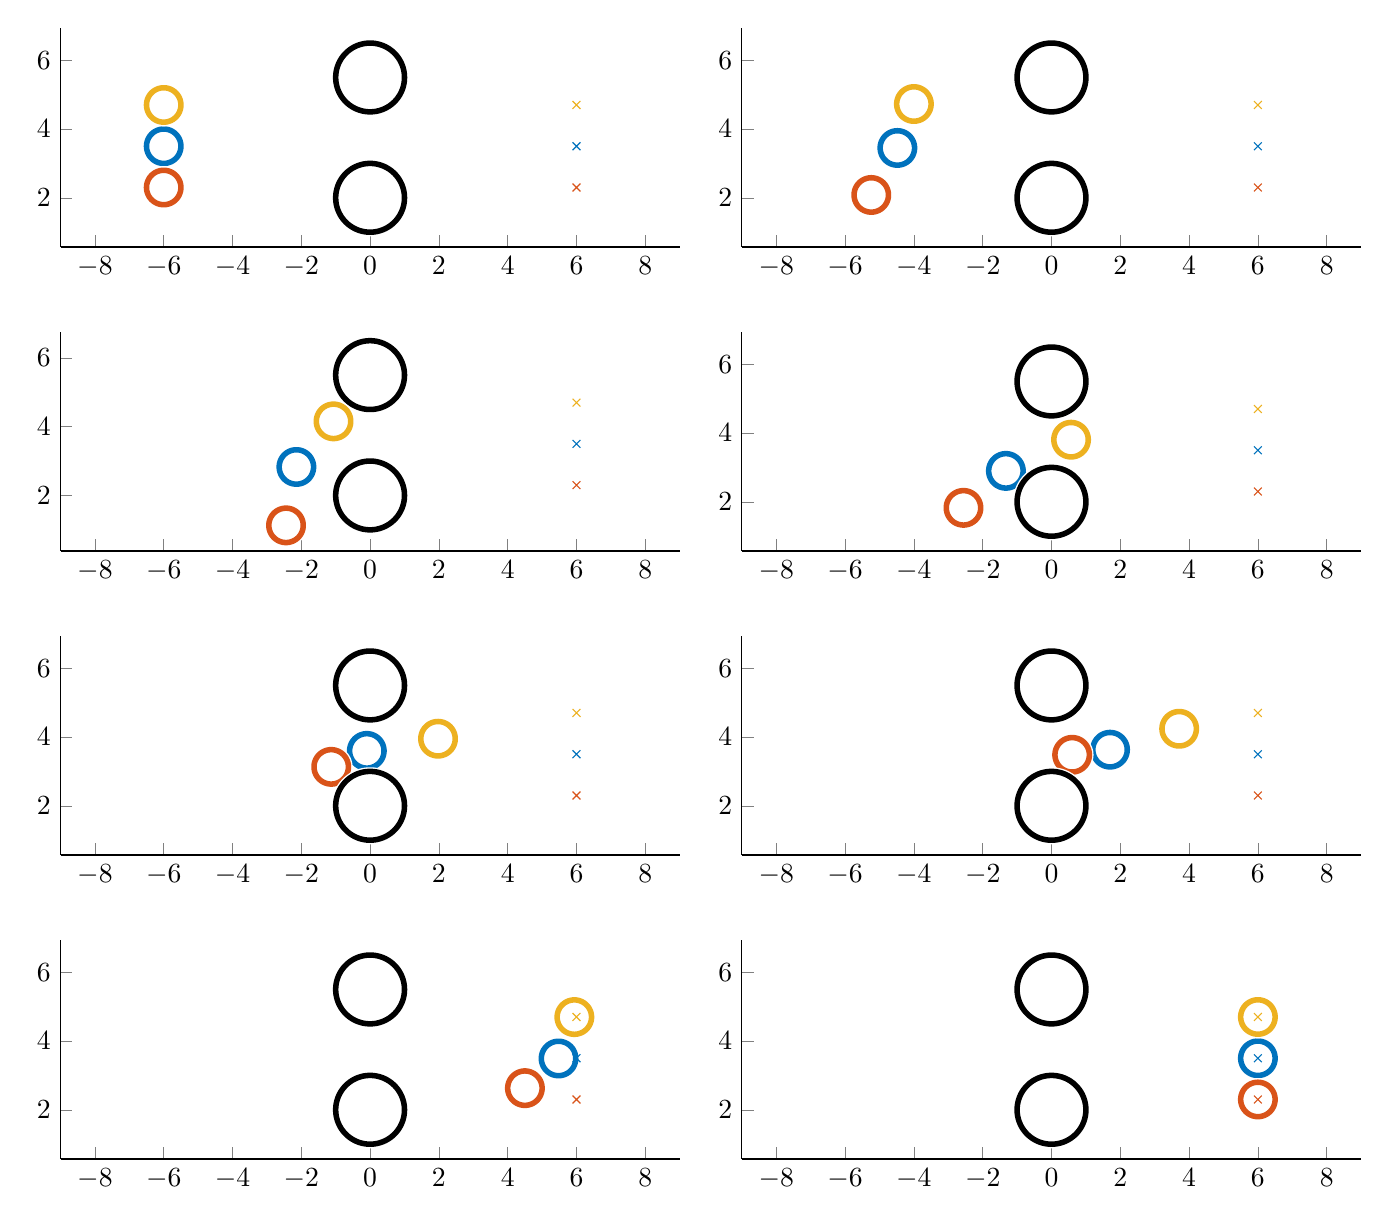
\begin{tikzpicture}

\definecolor{mycolor1}{rgb}{0.00000,0.44700,0.74100}%
\definecolor{mycolor2}{rgb}{0.85000,0.32500,0.09800}%
\definecolor{mycolor3}{rgb}{0.92900,0.69400,0.12500}%

\begin{axis}[%
width=3.096in,
height=1.094in,
at={(2.593in,5.323in)},
scale only axis,
unbounded coords=jump,
xmin=-9,
xmax=9,
%xmajorgrids,
ymin=0.568379976997646,
ymax=6.93162002300235,
%ymajorgrids,
axis background/.style={fill=white},
axis x line*=bottom,
axis y line*=left
]
\addplot [color=mycolor1,only marks,mark=x,mark options={solid},forget plot]
  table[row sep=crcr]{%
6	3.5\\
};
\addplot [color=mycolor2,only marks,mark=x,mark options={solid},forget plot]
  table[row sep=crcr]{%
6	2.3\\
};
\addplot [color=mycolor3,only marks,mark=x,mark options={solid},forget plot]
  table[row sep=crcr]{%
6	4.7\\
};
\addplot [color=white,solid,line width=3.0pt,forget plot]
  table[row sep=crcr]{%
-5.5	3.5\\
-5.50030458649045	3.51744974835125\\
-5.50121797487009	3.53487823687206\\
-5.50273905231586	3.55226423163383\\
-5.50486596562921	3.56958655048003\\
-5.5075961234939	3.58682408883347\\
-5.5109261996331	3.60395584540888\\
-5.514852136862	3.62096094779983\\
-5.51936915203084	3.6378186779085\\
-5.52447174185242	3.65450849718747\\
-5.53015368960705	3.67101007166283\\
-5.53640807271661	3.68730329670796\\
-5.5432272711787	3.7033683215379\\
-5.55060297685042	3.71918557339454\\
-5.55852620357054	3.73473578139295\\
-5.56698729810778	3.75\\
-5.57597595192179	3.7649596321166\\
-5.58548121372248	3.77959645173537\\
-5.59549150281253	3.79389262614624\\
-5.60599462319664	3.80783073766283\\
-5.61697777844051	3.82139380484327\\
-5.6284275872613	3.83456530317943\\
-5.64033009983067	3.8473291852295\\
-5.6526708147705	3.85966990016933\\
-5.66543469682057	3.8715724127387\\
-5.67860619515673	3.88302222155949\\
-5.69216926233717	3.89400537680336\\
-5.70610737385376	3.90450849718747\\
-5.72040354826463	3.91451878627752\\
-5.7350403678834	3.92402404807821\\
-5.75	3.93301270189222\\
-5.76526421860705	3.94147379642946\\
-5.78081442660546	3.94939702314958\\
-5.7966316784621	3.9567727288213\\
-5.81269670329204	3.96359192728339\\
-5.82898992833717	3.96984631039295\\
-5.84549150281253	3.97552825814758\\
-5.8621813220915	3.98063084796916\\
-5.87903905220017	3.985147863138\\
-5.89604415459112	3.9890738003669\\
-5.91317591116653	3.9924038765061\\
-5.93041344951997	3.99513403437079\\
-5.94773576836617	3.99726094768414\\
-5.96512176312794	3.99878202512991\\
-5.98255025164875	3.99969541350955\\
-6	4\\
-6.01744974835125	3.99969541350955\\
-6.03487823687206	3.99878202512991\\
-6.05226423163383	3.99726094768414\\
-6.06958655048003	3.99513403437079\\
-6.08682408883347	3.9924038765061\\
-6.10395584540888	3.9890738003669\\
-6.12096094779983	3.985147863138\\
-6.1378186779085	3.98063084796916\\
-6.15450849718747	3.97552825814758\\
-6.17101007166283	3.96984631039295\\
-6.18730329670796	3.96359192728339\\
-6.2033683215379	3.9567727288213\\
-6.21918557339454	3.94939702314958\\
-6.23473578139295	3.94147379642946\\
-6.25	3.93301270189222\\
-6.2649596321166	3.92402404807821\\
-6.27959645173537	3.91451878627752\\
-6.29389262614624	3.90450849718747\\
-6.30783073766283	3.89400537680336\\
-6.32139380484327	3.88302222155949\\
-6.33456530317943	3.8715724127387\\
-6.3473291852295	3.85966990016933\\
-6.35966990016933	3.8473291852295\\
-6.3715724127387	3.83456530317943\\
-6.38302222155949	3.82139380484327\\
-6.39400537680336	3.80783073766283\\
-6.40450849718747	3.79389262614624\\
-6.41451878627752	3.77959645173537\\
-6.42402404807821	3.7649596321166\\
-6.43301270189222	3.75\\
-6.44147379642946	3.73473578139295\\
-6.44939702314958	3.71918557339454\\
-6.4567727288213	3.7033683215379\\
-6.46359192728339	3.68730329670796\\
-6.46984631039295	3.67101007166283\\
-6.47552825814758	3.65450849718747\\
-6.48063084796916	3.6378186779085\\
-6.485147863138	3.62096094779983\\
-6.4890738003669	3.60395584540888\\
-6.4924038765061	3.58682408883347\\
-6.49513403437079	3.56958655048003\\
-6.49726094768414	3.55226423163383\\
-6.49878202512991	3.53487823687206\\
-6.49969541350955	3.51744974835125\\
-6.5	3.5\\
-6.49969541350955	3.48255025164875\\
-6.49878202512991	3.46512176312794\\
-6.49726094768414	3.44773576836617\\
-6.49513403437079	3.43041344951997\\
-6.4924038765061	3.41317591116653\\
-6.4890738003669	3.39604415459112\\
-6.485147863138	3.37903905220017\\
-6.48063084796916	3.3621813220915\\
-6.47552825814758	3.34549150281253\\
-6.46984631039295	3.32898992833717\\
-6.46359192728339	3.31269670329204\\
-6.4567727288213	3.2966316784621\\
-6.44939702314958	3.28081442660546\\
-6.44147379642946	3.26526421860705\\
-6.43301270189222	3.25\\
-6.42402404807821	3.2350403678834\\
-6.41451878627752	3.22040354826463\\
-6.40450849718747	3.20610737385376\\
-6.39400537680336	3.19216926233717\\
-6.38302222155949	3.17860619515673\\
-6.3715724127387	3.16543469682057\\
-6.35966990016933	3.1526708147705\\
-6.3473291852295	3.14033009983067\\
-6.33456530317943	3.1284275872613\\
-6.32139380484327	3.11697777844051\\
-6.30783073766283	3.10599462319664\\
-6.29389262614624	3.09549150281253\\
-6.27959645173537	3.08548121372248\\
-6.2649596321166	3.07597595192179\\
-6.25	3.06698729810778\\
-6.23473578139295	3.05852620357054\\
-6.21918557339454	3.05060297685042\\
-6.2033683215379	3.0432272711787\\
-6.18730329670796	3.03640807271661\\
-6.17101007166283	3.03015368960705\\
-6.15450849718747	3.02447174185242\\
-6.1378186779085	3.01936915203084\\
-6.12096094779983	3.014852136862\\
-6.10395584540888	3.0109261996331\\
-6.08682408883347	3.0075961234939\\
-6.06958655048003	3.00486596562921\\
-6.05226423163383	3.00273905231586\\
-6.03487823687206	3.00121797487009\\
-6.01744974835125	3.00030458649045\\
-6	3\\
-5.98255025164875	3.00030458649045\\
-5.96512176312794	3.00121797487009\\
-5.94773576836617	3.00273905231586\\
-5.93041344951997	3.00486596562921\\
-5.91317591116653	3.0075961234939\\
-5.89604415459112	3.0109261996331\\
-5.87903905220017	3.014852136862\\
-5.8621813220915	3.01936915203084\\
-5.84549150281253	3.02447174185242\\
-5.82898992833717	3.03015368960705\\
-5.81269670329204	3.03640807271661\\
-5.7966316784621	3.0432272711787\\
-5.78081442660546	3.05060297685042\\
-5.76526421860705	3.05852620357054\\
-5.75	3.06698729810778\\
-5.7350403678834	3.07597595192179\\
-5.72040354826463	3.08548121372248\\
-5.70610737385376	3.09549150281253\\
-5.69216926233717	3.10599462319664\\
-5.67860619515673	3.11697777844051\\
-5.66543469682057	3.1284275872613\\
-5.6526708147705	3.14033009983067\\
-5.64033009983067	3.1526708147705\\
-5.6284275872613	3.16543469682057\\
-5.61697777844051	3.17860619515673\\
-5.60599462319664	3.19216926233717\\
-5.59549150281253	3.20610737385376\\
-5.58548121372248	3.22040354826463\\
-5.57597595192179	3.2350403678834\\
-5.56698729810778	3.25\\
-5.55852620357054	3.26526421860705\\
-5.55060297685042	3.28081442660546\\
-5.5432272711787	3.2966316784621\\
-5.53640807271661	3.31269670329204\\
-5.53015368960705	3.32898992833717\\
-5.52447174185242	3.34549150281253\\
-5.51936915203084	3.3621813220915\\
-5.514852136862	3.37903905220017\\
-5.5109261996331	3.39604415459112\\
-5.5075961234939	3.41317591116653\\
-5.50486596562921	3.43041344951997\\
-5.50273905231586	3.44773576836617\\
-5.50121797487009	3.46512176312794\\
-5.50030458649045	3.48255025164875\\
-5.5	3.5\\
nan	nan\\
};
\addplot [color=mycolor1,solid,line width=2.0pt,forget plot]
  table[row sep=crcr]{%
-5.5	3.5\\
-5.50030458649045	3.51744974835125\\
-5.50121797487009	3.53487823687206\\
-5.50273905231586	3.55226423163383\\
-5.50486596562921	3.56958655048003\\
-5.5075961234939	3.58682408883347\\
-5.5109261996331	3.60395584540888\\
-5.514852136862	3.62096094779983\\
-5.51936915203084	3.6378186779085\\
-5.52447174185242	3.65450849718747\\
-5.53015368960705	3.67101007166283\\
-5.53640807271661	3.68730329670796\\
-5.5432272711787	3.7033683215379\\
-5.55060297685042	3.71918557339454\\
-5.55852620357054	3.73473578139295\\
-5.56698729810778	3.75\\
-5.57597595192179	3.7649596321166\\
-5.58548121372248	3.77959645173537\\
-5.59549150281253	3.79389262614624\\
-5.60599462319664	3.80783073766283\\
-5.61697777844051	3.82139380484327\\
-5.6284275872613	3.83456530317943\\
-5.64033009983067	3.8473291852295\\
-5.6526708147705	3.85966990016933\\
-5.66543469682057	3.8715724127387\\
-5.67860619515673	3.88302222155949\\
-5.69216926233717	3.89400537680336\\
-5.70610737385376	3.90450849718747\\
-5.72040354826463	3.91451878627752\\
-5.7350403678834	3.92402404807821\\
-5.75	3.93301270189222\\
-5.76526421860705	3.94147379642946\\
-5.78081442660546	3.94939702314958\\
-5.7966316784621	3.9567727288213\\
-5.81269670329204	3.96359192728339\\
-5.82898992833717	3.96984631039295\\
-5.84549150281253	3.97552825814758\\
-5.8621813220915	3.98063084796916\\
-5.87903905220017	3.985147863138\\
-5.89604415459112	3.9890738003669\\
-5.91317591116653	3.9924038765061\\
-5.93041344951997	3.99513403437079\\
-5.94773576836617	3.99726094768414\\
-5.96512176312794	3.99878202512991\\
-5.98255025164875	3.99969541350955\\
-6	4\\
-6.01744974835125	3.99969541350955\\
-6.03487823687206	3.99878202512991\\
-6.05226423163383	3.99726094768414\\
-6.06958655048003	3.99513403437079\\
-6.08682408883347	3.9924038765061\\
-6.10395584540888	3.9890738003669\\
-6.12096094779983	3.985147863138\\
-6.1378186779085	3.98063084796916\\
-6.15450849718747	3.97552825814758\\
-6.17101007166283	3.96984631039295\\
-6.18730329670796	3.96359192728339\\
-6.2033683215379	3.9567727288213\\
-6.21918557339454	3.94939702314958\\
-6.23473578139295	3.94147379642946\\
-6.25	3.93301270189222\\
-6.2649596321166	3.92402404807821\\
-6.27959645173537	3.91451878627752\\
-6.29389262614624	3.90450849718747\\
-6.30783073766283	3.89400537680336\\
-6.32139380484327	3.88302222155949\\
-6.33456530317943	3.8715724127387\\
-6.3473291852295	3.85966990016933\\
-6.35966990016933	3.8473291852295\\
-6.3715724127387	3.83456530317943\\
-6.38302222155949	3.82139380484327\\
-6.39400537680336	3.80783073766283\\
-6.40450849718747	3.79389262614624\\
-6.41451878627752	3.77959645173537\\
-6.42402404807821	3.7649596321166\\
-6.43301270189222	3.75\\
-6.44147379642946	3.73473578139295\\
-6.44939702314958	3.71918557339454\\
-6.4567727288213	3.7033683215379\\
-6.46359192728339	3.68730329670796\\
-6.46984631039295	3.67101007166283\\
-6.47552825814758	3.65450849718747\\
-6.48063084796916	3.6378186779085\\
-6.485147863138	3.62096094779983\\
-6.4890738003669	3.60395584540888\\
-6.4924038765061	3.58682408883347\\
-6.49513403437079	3.56958655048003\\
-6.49726094768414	3.55226423163383\\
-6.49878202512991	3.53487823687206\\
-6.49969541350955	3.51744974835125\\
-6.5	3.5\\
-6.49969541350955	3.48255025164875\\
-6.49878202512991	3.46512176312794\\
-6.49726094768414	3.44773576836617\\
-6.49513403437079	3.43041344951997\\
-6.4924038765061	3.41317591116653\\
-6.4890738003669	3.39604415459112\\
-6.485147863138	3.37903905220017\\
-6.48063084796916	3.3621813220915\\
-6.47552825814758	3.34549150281253\\
-6.46984631039295	3.32898992833717\\
-6.46359192728339	3.31269670329204\\
-6.4567727288213	3.2966316784621\\
-6.44939702314958	3.28081442660546\\
-6.44147379642946	3.26526421860705\\
-6.43301270189222	3.25\\
-6.42402404807821	3.2350403678834\\
-6.41451878627752	3.22040354826463\\
-6.40450849718747	3.20610737385376\\
-6.39400537680336	3.19216926233717\\
-6.38302222155949	3.17860619515673\\
-6.3715724127387	3.16543469682057\\
-6.35966990016933	3.1526708147705\\
-6.3473291852295	3.14033009983067\\
-6.33456530317943	3.1284275872613\\
-6.32139380484327	3.11697777844051\\
-6.30783073766283	3.10599462319664\\
-6.29389262614624	3.09549150281253\\
-6.27959645173537	3.08548121372248\\
-6.2649596321166	3.07597595192179\\
-6.25	3.06698729810778\\
-6.23473578139295	3.05852620357054\\
-6.21918557339454	3.05060297685042\\
-6.2033683215379	3.0432272711787\\
-6.18730329670796	3.03640807271661\\
-6.17101007166283	3.03015368960705\\
-6.15450849718747	3.02447174185242\\
-6.1378186779085	3.01936915203084\\
-6.12096094779983	3.014852136862\\
-6.10395584540888	3.0109261996331\\
-6.08682408883347	3.0075961234939\\
-6.06958655048003	3.00486596562921\\
-6.05226423163383	3.00273905231586\\
-6.03487823687206	3.00121797487009\\
-6.01744974835125	3.00030458649045\\
-6	3\\
-5.98255025164875	3.00030458649045\\
-5.96512176312794	3.00121797487009\\
-5.94773576836617	3.00273905231586\\
-5.93041344951997	3.00486596562921\\
-5.91317591116653	3.0075961234939\\
-5.89604415459112	3.0109261996331\\
-5.87903905220017	3.014852136862\\
-5.8621813220915	3.01936915203084\\
-5.84549150281253	3.02447174185242\\
-5.82898992833717	3.03015368960705\\
-5.81269670329204	3.03640807271661\\
-5.7966316784621	3.0432272711787\\
-5.78081442660546	3.05060297685042\\
-5.76526421860705	3.05852620357054\\
-5.75	3.06698729810778\\
-5.7350403678834	3.07597595192179\\
-5.72040354826463	3.08548121372248\\
-5.70610737385376	3.09549150281253\\
-5.69216926233717	3.10599462319664\\
-5.67860619515673	3.11697777844051\\
-5.66543469682057	3.1284275872613\\
-5.6526708147705	3.14033009983067\\
-5.64033009983067	3.1526708147705\\
-5.6284275872613	3.16543469682057\\
-5.61697777844051	3.17860619515673\\
-5.60599462319664	3.19216926233717\\
-5.59549150281253	3.20610737385376\\
-5.58548121372248	3.22040354826463\\
-5.57597595192179	3.2350403678834\\
-5.56698729810778	3.25\\
-5.55852620357054	3.26526421860705\\
-5.55060297685042	3.28081442660546\\
-5.5432272711787	3.2966316784621\\
-5.53640807271661	3.31269670329204\\
-5.53015368960705	3.32898992833717\\
-5.52447174185242	3.34549150281253\\
-5.51936915203084	3.3621813220915\\
-5.514852136862	3.37903905220017\\
-5.5109261996331	3.39604415459112\\
-5.5075961234939	3.41317591116653\\
-5.50486596562921	3.43041344951997\\
-5.50273905231586	3.44773576836617\\
-5.50121797487009	3.46512176312794\\
-5.50030458649045	3.48255025164875\\
-5.5	3.5\\
nan	nan\\
};
\addplot [color=white,solid,line width=3.0pt,forget plot]
  table[row sep=crcr]{%
-5.5	2.3\\
-5.50030458649045	2.31744974835125\\
-5.50121797487009	2.33487823687206\\
-5.50273905231586	2.35226423163383\\
-5.50486596562921	2.36958655048003\\
-5.5075961234939	2.38682408883346\\
-5.5109261996331	2.40395584540888\\
-5.514852136862	2.42096094779983\\
-5.51936915203084	2.4378186779085\\
-5.52447174185242	2.45450849718747\\
-5.53015368960705	2.47101007166283\\
-5.53640807271661	2.48730329670796\\
-5.5432272711787	2.5033683215379\\
-5.55060297685042	2.51918557339454\\
-5.55852620357054	2.53473578139295\\
-5.56698729810778	2.55\\
-5.57597595192179	2.5649596321166\\
-5.58548121372248	2.57959645173537\\
-5.59549150281253	2.59389262614624\\
-5.60599462319664	2.60783073766283\\
-5.61697777844051	2.62139380484327\\
-5.6284275872613	2.63456530317943\\
-5.64033009983067	2.6473291852295\\
-5.6526708147705	2.65966990016933\\
-5.66543469682057	2.6715724127387\\
-5.67860619515673	2.68302222155949\\
-5.69216926233717	2.69400537680336\\
-5.70610737385376	2.70450849718747\\
-5.72040354826463	2.71451878627752\\
-5.7350403678834	2.72402404807821\\
-5.75	2.73301270189222\\
-5.76526421860705	2.74147379642946\\
-5.78081442660546	2.74939702314958\\
-5.7966316784621	2.7567727288213\\
-5.81269670329204	2.76359192728339\\
-5.82898992833717	2.76984631039295\\
-5.84549150281253	2.77552825814758\\
-5.8621813220915	2.78063084796916\\
-5.87903905220017	2.785147863138\\
-5.89604415459112	2.7890738003669\\
-5.91317591116653	2.7924038765061\\
-5.93041344951997	2.79513403437078\\
-5.94773576836617	2.79726094768414\\
-5.96512176312794	2.79878202512991\\
-5.98255025164875	2.79969541350955\\
-6	2.8\\
-6.01744974835125	2.79969541350955\\
-6.03487823687206	2.79878202512991\\
-6.05226423163383	2.79726094768414\\
-6.06958655048003	2.79513403437078\\
-6.08682408883347	2.7924038765061\\
-6.10395584540888	2.7890738003669\\
-6.12096094779983	2.785147863138\\
-6.1378186779085	2.78063084796916\\
-6.15450849718747	2.77552825814758\\
-6.17101007166283	2.76984631039295\\
-6.18730329670796	2.76359192728339\\
-6.2033683215379	2.7567727288213\\
-6.21918557339454	2.74939702314958\\
-6.23473578139295	2.74147379642946\\
-6.25	2.73301270189222\\
-6.2649596321166	2.72402404807821\\
-6.27959645173537	2.71451878627752\\
-6.29389262614624	2.70450849718747\\
-6.30783073766283	2.69400537680336\\
-6.32139380484327	2.68302222155949\\
-6.33456530317943	2.6715724127387\\
-6.3473291852295	2.65966990016933\\
-6.35966990016933	2.6473291852295\\
-6.3715724127387	2.63456530317943\\
-6.38302222155949	2.62139380484327\\
-6.39400537680336	2.60783073766283\\
-6.40450849718747	2.59389262614624\\
-6.41451878627752	2.57959645173537\\
-6.42402404807821	2.5649596321166\\
-6.43301270189222	2.55\\
-6.44147379642946	2.53473578139295\\
-6.44939702314958	2.51918557339454\\
-6.4567727288213	2.5033683215379\\
-6.46359192728339	2.48730329670796\\
-6.46984631039295	2.47101007166283\\
-6.47552825814758	2.45450849718747\\
-6.48063084796916	2.4378186779085\\
-6.485147863138	2.42096094779983\\
-6.4890738003669	2.40395584540888\\
-6.4924038765061	2.38682408883346\\
-6.49513403437079	2.36958655048003\\
-6.49726094768414	2.35226423163383\\
-6.49878202512991	2.33487823687206\\
-6.49969541350955	2.31744974835125\\
-6.5	2.3\\
-6.49969541350955	2.28255025164875\\
-6.49878202512991	2.26512176312794\\
-6.49726094768414	2.24773576836617\\
-6.49513403437079	2.23041344951997\\
-6.4924038765061	2.21317591116653\\
-6.4890738003669	2.19604415459112\\
-6.485147863138	2.17903905220017\\
-6.48063084796916	2.1621813220915\\
-6.47552825814758	2.14549150281253\\
-6.46984631039295	2.12898992833717\\
-6.46359192728339	2.11269670329204\\
-6.4567727288213	2.0966316784621\\
-6.44939702314958	2.08081442660546\\
-6.44147379642946	2.06526421860705\\
-6.43301270189222	2.05\\
-6.42402404807821	2.0350403678834\\
-6.41451878627752	2.02040354826463\\
-6.40450849718747	2.00610737385376\\
-6.39400537680336	1.99216926233717\\
-6.38302222155949	1.97860619515673\\
-6.3715724127387	1.96543469682057\\
-6.35966990016933	1.9526708147705\\
-6.3473291852295	1.94033009983067\\
-6.33456530317943	1.9284275872613\\
-6.32139380484327	1.91697777844051\\
-6.30783073766283	1.90599462319664\\
-6.29389262614624	1.89549150281253\\
-6.27959645173537	1.88548121372248\\
-6.2649596321166	1.87597595192179\\
-6.25	1.86698729810778\\
-6.23473578139295	1.85852620357054\\
-6.21918557339454	1.85060297685042\\
-6.2033683215379	1.8432272711787\\
-6.18730329670796	1.83640807271661\\
-6.17101007166283	1.83015368960705\\
-6.15450849718747	1.82447174185242\\
-6.1378186779085	1.81936915203084\\
-6.12096094779983	1.814852136862\\
-6.10395584540888	1.8109261996331\\
-6.08682408883347	1.8075961234939\\
-6.06958655048003	1.80486596562921\\
-6.05226423163383	1.80273905231586\\
-6.03487823687206	1.80121797487009\\
-6.01744974835125	1.80030458649045\\
-6	1.8\\
-5.98255025164875	1.80030458649045\\
-5.96512176312794	1.80121797487009\\
-5.94773576836617	1.80273905231586\\
-5.93041344951997	1.80486596562921\\
-5.91317591116653	1.8075961234939\\
-5.89604415459112	1.8109261996331\\
-5.87903905220017	1.814852136862\\
-5.8621813220915	1.81936915203084\\
-5.84549150281253	1.82447174185242\\
-5.82898992833717	1.83015368960705\\
-5.81269670329204	1.83640807271661\\
-5.7966316784621	1.8432272711787\\
-5.78081442660546	1.85060297685042\\
-5.76526421860705	1.85852620357054\\
-5.75	1.86698729810778\\
-5.7350403678834	1.87597595192179\\
-5.72040354826463	1.88548121372248\\
-5.70610737385376	1.89549150281253\\
-5.69216926233717	1.90599462319664\\
-5.67860619515673	1.91697777844051\\
-5.66543469682057	1.9284275872613\\
-5.6526708147705	1.94033009983067\\
-5.64033009983067	1.9526708147705\\
-5.6284275872613	1.96543469682057\\
-5.61697777844051	1.97860619515673\\
-5.60599462319664	1.99216926233717\\
-5.59549150281253	2.00610737385376\\
-5.58548121372248	2.02040354826463\\
-5.57597595192179	2.0350403678834\\
-5.56698729810778	2.05\\
-5.55852620357054	2.06526421860705\\
-5.55060297685042	2.08081442660546\\
-5.5432272711787	2.0966316784621\\
-5.53640807271661	2.11269670329204\\
-5.53015368960705	2.12898992833717\\
-5.52447174185242	2.14549150281253\\
-5.51936915203084	2.1621813220915\\
-5.514852136862	2.17903905220017\\
-5.5109261996331	2.19604415459112\\
-5.5075961234939	2.21317591116653\\
-5.50486596562921	2.23041344951997\\
-5.50273905231586	2.24773576836617\\
-5.50121797487009	2.26512176312794\\
-5.50030458649045	2.28255025164875\\
-5.5	2.3\\
nan	nan\\
};
\addplot [color=mycolor2,solid,line width=2.0pt,forget plot]
  table[row sep=crcr]{%
-5.5	2.3\\
-5.50030458649045	2.31744974835125\\
-5.50121797487009	2.33487823687206\\
-5.50273905231586	2.35226423163383\\
-5.50486596562921	2.36958655048003\\
-5.5075961234939	2.38682408883346\\
-5.5109261996331	2.40395584540888\\
-5.514852136862	2.42096094779983\\
-5.51936915203084	2.4378186779085\\
-5.52447174185242	2.45450849718747\\
-5.53015368960705	2.47101007166283\\
-5.53640807271661	2.48730329670796\\
-5.5432272711787	2.5033683215379\\
-5.55060297685042	2.51918557339454\\
-5.55852620357054	2.53473578139295\\
-5.56698729810778	2.55\\
-5.57597595192179	2.5649596321166\\
-5.58548121372248	2.57959645173537\\
-5.59549150281253	2.59389262614624\\
-5.60599462319664	2.60783073766283\\
-5.61697777844051	2.62139380484327\\
-5.6284275872613	2.63456530317943\\
-5.64033009983067	2.6473291852295\\
-5.6526708147705	2.65966990016933\\
-5.66543469682057	2.6715724127387\\
-5.67860619515673	2.68302222155949\\
-5.69216926233717	2.69400537680336\\
-5.70610737385376	2.70450849718747\\
-5.72040354826463	2.71451878627752\\
-5.7350403678834	2.72402404807821\\
-5.75	2.73301270189222\\
-5.76526421860705	2.74147379642946\\
-5.78081442660546	2.74939702314958\\
-5.7966316784621	2.7567727288213\\
-5.81269670329204	2.76359192728339\\
-5.82898992833717	2.76984631039295\\
-5.84549150281253	2.77552825814758\\
-5.8621813220915	2.78063084796916\\
-5.87903905220017	2.785147863138\\
-5.89604415459112	2.7890738003669\\
-5.91317591116653	2.7924038765061\\
-5.93041344951997	2.79513403437078\\
-5.94773576836617	2.79726094768414\\
-5.96512176312794	2.79878202512991\\
-5.98255025164875	2.79969541350955\\
-6	2.8\\
-6.01744974835125	2.79969541350955\\
-6.03487823687206	2.79878202512991\\
-6.05226423163383	2.79726094768414\\
-6.06958655048003	2.79513403437078\\
-6.08682408883347	2.7924038765061\\
-6.10395584540888	2.7890738003669\\
-6.12096094779983	2.785147863138\\
-6.1378186779085	2.78063084796916\\
-6.15450849718747	2.77552825814758\\
-6.17101007166283	2.76984631039295\\
-6.18730329670796	2.76359192728339\\
-6.2033683215379	2.7567727288213\\
-6.21918557339454	2.74939702314958\\
-6.23473578139295	2.74147379642946\\
-6.25	2.73301270189222\\
-6.2649596321166	2.72402404807821\\
-6.27959645173537	2.71451878627752\\
-6.29389262614624	2.70450849718747\\
-6.30783073766283	2.69400537680336\\
-6.32139380484327	2.68302222155949\\
-6.33456530317943	2.6715724127387\\
-6.3473291852295	2.65966990016933\\
-6.35966990016933	2.6473291852295\\
-6.3715724127387	2.63456530317943\\
-6.38302222155949	2.62139380484327\\
-6.39400537680336	2.60783073766283\\
-6.40450849718747	2.59389262614624\\
-6.41451878627752	2.57959645173537\\
-6.42402404807821	2.5649596321166\\
-6.43301270189222	2.55\\
-6.44147379642946	2.53473578139295\\
-6.44939702314958	2.51918557339454\\
-6.4567727288213	2.5033683215379\\
-6.46359192728339	2.48730329670796\\
-6.46984631039295	2.47101007166283\\
-6.47552825814758	2.45450849718747\\
-6.48063084796916	2.4378186779085\\
-6.485147863138	2.42096094779983\\
-6.4890738003669	2.40395584540888\\
-6.4924038765061	2.38682408883346\\
-6.49513403437079	2.36958655048003\\
-6.49726094768414	2.35226423163383\\
-6.49878202512991	2.33487823687206\\
-6.49969541350955	2.31744974835125\\
-6.5	2.3\\
-6.49969541350955	2.28255025164875\\
-6.49878202512991	2.26512176312794\\
-6.49726094768414	2.24773576836617\\
-6.49513403437079	2.23041344951997\\
-6.4924038765061	2.21317591116653\\
-6.4890738003669	2.19604415459112\\
-6.485147863138	2.17903905220017\\
-6.48063084796916	2.1621813220915\\
-6.47552825814758	2.14549150281253\\
-6.46984631039295	2.12898992833717\\
-6.46359192728339	2.11269670329204\\
-6.4567727288213	2.0966316784621\\
-6.44939702314958	2.08081442660546\\
-6.44147379642946	2.06526421860705\\
-6.43301270189222	2.05\\
-6.42402404807821	2.0350403678834\\
-6.41451878627752	2.02040354826463\\
-6.40450849718747	2.00610737385376\\
-6.39400537680336	1.99216926233717\\
-6.38302222155949	1.97860619515673\\
-6.3715724127387	1.96543469682057\\
-6.35966990016933	1.9526708147705\\
-6.3473291852295	1.94033009983067\\
-6.33456530317943	1.9284275872613\\
-6.32139380484327	1.91697777844051\\
-6.30783073766283	1.90599462319664\\
-6.29389262614624	1.89549150281253\\
-6.27959645173537	1.88548121372248\\
-6.2649596321166	1.87597595192179\\
-6.25	1.86698729810778\\
-6.23473578139295	1.85852620357054\\
-6.21918557339454	1.85060297685042\\
-6.2033683215379	1.8432272711787\\
-6.18730329670796	1.83640807271661\\
-6.17101007166283	1.83015368960705\\
-6.15450849718747	1.82447174185242\\
-6.1378186779085	1.81936915203084\\
-6.12096094779983	1.814852136862\\
-6.10395584540888	1.8109261996331\\
-6.08682408883347	1.8075961234939\\
-6.06958655048003	1.80486596562921\\
-6.05226423163383	1.80273905231586\\
-6.03487823687206	1.80121797487009\\
-6.01744974835125	1.80030458649045\\
-6	1.8\\
-5.98255025164875	1.80030458649045\\
-5.96512176312794	1.80121797487009\\
-5.94773576836617	1.80273905231586\\
-5.93041344951997	1.80486596562921\\
-5.91317591116653	1.8075961234939\\
-5.89604415459112	1.8109261996331\\
-5.87903905220017	1.814852136862\\
-5.8621813220915	1.81936915203084\\
-5.84549150281253	1.82447174185242\\
-5.82898992833717	1.83015368960705\\
-5.81269670329204	1.83640807271661\\
-5.7966316784621	1.8432272711787\\
-5.78081442660546	1.85060297685042\\
-5.76526421860705	1.85852620357054\\
-5.75	1.86698729810778\\
-5.7350403678834	1.87597595192179\\
-5.72040354826463	1.88548121372248\\
-5.70610737385376	1.89549150281253\\
-5.69216926233717	1.90599462319664\\
-5.67860619515673	1.91697777844051\\
-5.66543469682057	1.9284275872613\\
-5.6526708147705	1.94033009983067\\
-5.64033009983067	1.9526708147705\\
-5.6284275872613	1.96543469682057\\
-5.61697777844051	1.97860619515673\\
-5.60599462319664	1.99216926233717\\
-5.59549150281253	2.00610737385376\\
-5.58548121372248	2.02040354826463\\
-5.57597595192179	2.0350403678834\\
-5.56698729810778	2.05\\
-5.55852620357054	2.06526421860705\\
-5.55060297685042	2.08081442660546\\
-5.5432272711787	2.0966316784621\\
-5.53640807271661	2.11269670329204\\
-5.53015368960705	2.12898992833717\\
-5.52447174185242	2.14549150281253\\
-5.51936915203084	2.1621813220915\\
-5.514852136862	2.17903905220017\\
-5.5109261996331	2.19604415459112\\
-5.5075961234939	2.21317591116653\\
-5.50486596562921	2.23041344951997\\
-5.50273905231586	2.24773576836617\\
-5.50121797487009	2.26512176312794\\
-5.50030458649045	2.28255025164875\\
-5.5	2.3\\
nan	nan\\
};
\addplot [color=white,solid,line width=3.0pt,forget plot]
  table[row sep=crcr]{%
-5.5	4.7\\
-5.50030458649045	4.71744974835125\\
-5.50121797487009	4.73487823687206\\
-5.50273905231586	4.75226423163383\\
-5.50486596562921	4.76958655048003\\
-5.5075961234939	4.78682408883347\\
-5.5109261996331	4.80395584540888\\
-5.514852136862	4.82096094779983\\
-5.51936915203084	4.8378186779085\\
-5.52447174185242	4.85450849718747\\
-5.53015368960705	4.87101007166283\\
-5.53640807271661	4.88730329670796\\
-5.5432272711787	4.9033683215379\\
-5.55060297685042	4.91918557339454\\
-5.55852620357054	4.93473578139295\\
-5.56698729810778	4.95\\
-5.57597595192179	4.9649596321166\\
-5.58548121372248	4.97959645173537\\
-5.59549150281253	4.99389262614624\\
-5.60599462319664	5.00783073766283\\
-5.61697777844051	5.02139380484327\\
-5.6284275872613	5.03456530317943\\
-5.64033009983067	5.0473291852295\\
-5.6526708147705	5.05966990016933\\
-5.66543469682057	5.0715724127387\\
-5.67860619515673	5.08302222155949\\
-5.69216926233717	5.09400537680336\\
-5.70610737385376	5.10450849718747\\
-5.72040354826463	5.11451878627752\\
-5.7350403678834	5.12402404807821\\
-5.75	5.13301270189222\\
-5.76526421860705	5.14147379642946\\
-5.78081442660546	5.14939702314958\\
-5.7966316784621	5.1567727288213\\
-5.81269670329204	5.16359192728339\\
-5.82898992833717	5.16984631039295\\
-5.84549150281253	5.17552825814758\\
-5.8621813220915	5.18063084796916\\
-5.87903905220017	5.185147863138\\
-5.89604415459112	5.1890738003669\\
-5.91317591116653	5.1924038765061\\
-5.93041344951997	5.19513403437079\\
-5.94773576836617	5.19726094768414\\
-5.96512176312794	5.19878202512991\\
-5.98255025164875	5.19969541350955\\
-6	5.2\\
-6.01744974835125	5.19969541350955\\
-6.03487823687206	5.19878202512991\\
-6.05226423163383	5.19726094768414\\
-6.06958655048003	5.19513403437079\\
-6.08682408883347	5.1924038765061\\
-6.10395584540888	5.1890738003669\\
-6.12096094779983	5.185147863138\\
-6.1378186779085	5.18063084796916\\
-6.15450849718747	5.17552825814758\\
-6.17101007166283	5.16984631039295\\
-6.18730329670796	5.16359192728339\\
-6.2033683215379	5.1567727288213\\
-6.21918557339454	5.14939702314958\\
-6.23473578139295	5.14147379642946\\
-6.25	5.13301270189222\\
-6.2649596321166	5.12402404807821\\
-6.27959645173537	5.11451878627752\\
-6.29389262614624	5.10450849718747\\
-6.30783073766283	5.09400537680336\\
-6.32139380484327	5.08302222155949\\
-6.33456530317943	5.0715724127387\\
-6.3473291852295	5.05966990016933\\
-6.35966990016933	5.0473291852295\\
-6.3715724127387	5.03456530317943\\
-6.38302222155949	5.02139380484327\\
-6.39400537680336	5.00783073766283\\
-6.40450849718747	4.99389262614624\\
-6.41451878627752	4.97959645173537\\
-6.42402404807821	4.9649596321166\\
-6.43301270189222	4.95\\
-6.44147379642946	4.93473578139295\\
-6.44939702314958	4.91918557339454\\
-6.4567727288213	4.9033683215379\\
-6.46359192728339	4.88730329670796\\
-6.46984631039295	4.87101007166283\\
-6.47552825814758	4.85450849718747\\
-6.48063084796916	4.8378186779085\\
-6.485147863138	4.82096094779983\\
-6.4890738003669	4.80395584540888\\
-6.4924038765061	4.78682408883347\\
-6.49513403437079	4.76958655048003\\
-6.49726094768414	4.75226423163383\\
-6.49878202512991	4.73487823687206\\
-6.49969541350955	4.71744974835125\\
-6.5	4.7\\
-6.49969541350955	4.68255025164875\\
-6.49878202512991	4.66512176312794\\
-6.49726094768414	4.64773576836617\\
-6.49513403437079	4.63041344951997\\
-6.4924038765061	4.61317591116654\\
-6.4890738003669	4.59604415459112\\
-6.485147863138	4.57903905220017\\
-6.48063084796916	4.5621813220915\\
-6.47552825814758	4.54549150281253\\
-6.46984631039295	4.52898992833717\\
-6.46359192728339	4.51269670329204\\
-6.4567727288213	4.4966316784621\\
-6.44939702314958	4.48081442660546\\
-6.44147379642946	4.46526421860705\\
-6.43301270189222	4.45\\
-6.42402404807821	4.4350403678834\\
-6.41451878627752	4.42040354826463\\
-6.40450849718747	4.40610737385376\\
-6.39400537680336	4.39216926233717\\
-6.38302222155949	4.37860619515673\\
-6.3715724127387	4.36543469682057\\
-6.35966990016933	4.3526708147705\\
-6.3473291852295	4.34033009983068\\
-6.33456530317943	4.3284275872613\\
-6.32139380484327	4.31697777844051\\
-6.30783073766283	4.30599462319664\\
-6.29389262614624	4.29549150281253\\
-6.27959645173537	4.28548121372248\\
-6.2649596321166	4.27597595192179\\
-6.25	4.26698729810778\\
-6.23473578139295	4.25852620357054\\
-6.21918557339454	4.25060297685042\\
-6.2033683215379	4.2432272711787\\
-6.18730329670796	4.23640807271661\\
-6.17101007166283	4.23015368960705\\
-6.15450849718747	4.22447174185242\\
-6.1378186779085	4.21936915203084\\
-6.12096094779983	4.214852136862\\
-6.10395584540888	4.2109261996331\\
-6.08682408883347	4.2075961234939\\
-6.06958655048003	4.20486596562921\\
-6.05226423163383	4.20273905231586\\
-6.03487823687206	4.20121797487009\\
-6.01744974835125	4.20030458649045\\
-6	4.2\\
-5.98255025164875	4.20030458649045\\
-5.96512176312794	4.20121797487009\\
-5.94773576836617	4.20273905231586\\
-5.93041344951997	4.20486596562921\\
-5.91317591116653	4.2075961234939\\
-5.89604415459112	4.2109261996331\\
-5.87903905220017	4.214852136862\\
-5.8621813220915	4.21936915203084\\
-5.84549150281253	4.22447174185242\\
-5.82898992833717	4.23015368960705\\
-5.81269670329204	4.23640807271661\\
-5.7966316784621	4.2432272711787\\
-5.78081442660546	4.25060297685042\\
-5.76526421860705	4.25852620357054\\
-5.75	4.26698729810778\\
-5.7350403678834	4.27597595192179\\
-5.72040354826463	4.28548121372248\\
-5.70610737385376	4.29549150281253\\
-5.69216926233717	4.30599462319664\\
-5.67860619515673	4.31697777844051\\
-5.66543469682057	4.3284275872613\\
-5.6526708147705	4.34033009983067\\
-5.64033009983067	4.3526708147705\\
-5.6284275872613	4.36543469682057\\
-5.61697777844051	4.37860619515673\\
-5.60599462319664	4.39216926233717\\
-5.59549150281253	4.40610737385376\\
-5.58548121372248	4.42040354826463\\
-5.57597595192179	4.4350403678834\\
-5.56698729810778	4.45\\
-5.55852620357054	4.46526421860705\\
-5.55060297685042	4.48081442660546\\
-5.5432272711787	4.4966316784621\\
-5.53640807271661	4.51269670329204\\
-5.53015368960705	4.52898992833717\\
-5.52447174185242	4.54549150281253\\
-5.51936915203084	4.5621813220915\\
-5.514852136862	4.57903905220017\\
-5.5109261996331	4.59604415459112\\
-5.5075961234939	4.61317591116653\\
-5.50486596562921	4.63041344951997\\
-5.50273905231586	4.64773576836617\\
-5.50121797487009	4.66512176312794\\
-5.50030458649045	4.68255025164875\\
-5.5	4.7\\
nan	nan\\
};
\addplot [color=mycolor3,solid,line width=2.0pt,forget plot]
  table[row sep=crcr]{%
-5.5	4.7\\
-5.50030458649045	4.71744974835125\\
-5.50121797487009	4.73487823687206\\
-5.50273905231586	4.75226423163383\\
-5.50486596562921	4.76958655048003\\
-5.5075961234939	4.78682408883347\\
-5.5109261996331	4.80395584540888\\
-5.514852136862	4.82096094779983\\
-5.51936915203084	4.8378186779085\\
-5.52447174185242	4.85450849718747\\
-5.53015368960705	4.87101007166283\\
-5.53640807271661	4.88730329670796\\
-5.5432272711787	4.9033683215379\\
-5.55060297685042	4.91918557339454\\
-5.55852620357054	4.93473578139295\\
-5.56698729810778	4.95\\
-5.57597595192179	4.9649596321166\\
-5.58548121372248	4.97959645173537\\
-5.59549150281253	4.99389262614624\\
-5.60599462319664	5.00783073766283\\
-5.61697777844051	5.02139380484327\\
-5.6284275872613	5.03456530317943\\
-5.64033009983067	5.0473291852295\\
-5.6526708147705	5.05966990016933\\
-5.66543469682057	5.0715724127387\\
-5.67860619515673	5.08302222155949\\
-5.69216926233717	5.09400537680336\\
-5.70610737385376	5.10450849718747\\
-5.72040354826463	5.11451878627752\\
-5.7350403678834	5.12402404807821\\
-5.75	5.13301270189222\\
-5.76526421860705	5.14147379642946\\
-5.78081442660546	5.14939702314958\\
-5.7966316784621	5.1567727288213\\
-5.81269670329204	5.16359192728339\\
-5.82898992833717	5.16984631039295\\
-5.84549150281253	5.17552825814758\\
-5.8621813220915	5.18063084796916\\
-5.87903905220017	5.185147863138\\
-5.89604415459112	5.1890738003669\\
-5.91317591116653	5.1924038765061\\
-5.93041344951997	5.19513403437079\\
-5.94773576836617	5.19726094768414\\
-5.96512176312794	5.19878202512991\\
-5.98255025164875	5.19969541350955\\
-6	5.2\\
-6.01744974835125	5.19969541350955\\
-6.03487823687206	5.19878202512991\\
-6.05226423163383	5.19726094768414\\
-6.06958655048003	5.19513403437079\\
-6.08682408883347	5.1924038765061\\
-6.10395584540888	5.1890738003669\\
-6.12096094779983	5.185147863138\\
-6.1378186779085	5.18063084796916\\
-6.15450849718747	5.17552825814758\\
-6.17101007166283	5.16984631039295\\
-6.18730329670796	5.16359192728339\\
-6.2033683215379	5.1567727288213\\
-6.21918557339454	5.14939702314958\\
-6.23473578139295	5.14147379642946\\
-6.25	5.13301270189222\\
-6.2649596321166	5.12402404807821\\
-6.27959645173537	5.11451878627752\\
-6.29389262614624	5.10450849718747\\
-6.30783073766283	5.09400537680336\\
-6.32139380484327	5.08302222155949\\
-6.33456530317943	5.0715724127387\\
-6.3473291852295	5.05966990016933\\
-6.35966990016933	5.0473291852295\\
-6.3715724127387	5.03456530317943\\
-6.38302222155949	5.02139380484327\\
-6.39400537680336	5.00783073766283\\
-6.40450849718747	4.99389262614624\\
-6.41451878627752	4.97959645173537\\
-6.42402404807821	4.9649596321166\\
-6.43301270189222	4.95\\
-6.44147379642946	4.93473578139295\\
-6.44939702314958	4.91918557339454\\
-6.4567727288213	4.9033683215379\\
-6.46359192728339	4.88730329670796\\
-6.46984631039295	4.87101007166283\\
-6.47552825814758	4.85450849718747\\
-6.48063084796916	4.8378186779085\\
-6.485147863138	4.82096094779983\\
-6.4890738003669	4.80395584540888\\
-6.4924038765061	4.78682408883347\\
-6.49513403437079	4.76958655048003\\
-6.49726094768414	4.75226423163383\\
-6.49878202512991	4.73487823687206\\
-6.49969541350955	4.71744974835125\\
-6.5	4.7\\
-6.49969541350955	4.68255025164875\\
-6.49878202512991	4.66512176312794\\
-6.49726094768414	4.64773576836617\\
-6.49513403437079	4.63041344951997\\
-6.4924038765061	4.61317591116654\\
-6.4890738003669	4.59604415459112\\
-6.485147863138	4.57903905220017\\
-6.48063084796916	4.5621813220915\\
-6.47552825814758	4.54549150281253\\
-6.46984631039295	4.52898992833717\\
-6.46359192728339	4.51269670329204\\
-6.4567727288213	4.4966316784621\\
-6.44939702314958	4.48081442660546\\
-6.44147379642946	4.46526421860705\\
-6.43301270189222	4.45\\
-6.42402404807821	4.4350403678834\\
-6.41451878627752	4.42040354826463\\
-6.40450849718747	4.40610737385376\\
-6.39400537680336	4.39216926233717\\
-6.38302222155949	4.37860619515673\\
-6.3715724127387	4.36543469682057\\
-6.35966990016933	4.3526708147705\\
-6.3473291852295	4.34033009983068\\
-6.33456530317943	4.3284275872613\\
-6.32139380484327	4.31697777844051\\
-6.30783073766283	4.30599462319664\\
-6.29389262614624	4.29549150281253\\
-6.27959645173537	4.28548121372248\\
-6.2649596321166	4.27597595192179\\
-6.25	4.26698729810778\\
-6.23473578139295	4.25852620357054\\
-6.21918557339454	4.25060297685042\\
-6.2033683215379	4.2432272711787\\
-6.18730329670796	4.23640807271661\\
-6.17101007166283	4.23015368960705\\
-6.15450849718747	4.22447174185242\\
-6.1378186779085	4.21936915203084\\
-6.12096094779983	4.214852136862\\
-6.10395584540888	4.2109261996331\\
-6.08682408883347	4.2075961234939\\
-6.06958655048003	4.20486596562921\\
-6.05226423163383	4.20273905231586\\
-6.03487823687206	4.20121797487009\\
-6.01744974835125	4.20030458649045\\
-6	4.2\\
-5.98255025164875	4.20030458649045\\
-5.96512176312794	4.20121797487009\\
-5.94773576836617	4.20273905231586\\
-5.93041344951997	4.20486596562921\\
-5.91317591116653	4.2075961234939\\
-5.89604415459112	4.2109261996331\\
-5.87903905220017	4.214852136862\\
-5.8621813220915	4.21936915203084\\
-5.84549150281253	4.22447174185242\\
-5.82898992833717	4.23015368960705\\
-5.81269670329204	4.23640807271661\\
-5.7966316784621	4.2432272711787\\
-5.78081442660546	4.25060297685042\\
-5.76526421860705	4.25852620357054\\
-5.75	4.26698729810778\\
-5.7350403678834	4.27597595192179\\
-5.72040354826463	4.28548121372248\\
-5.70610737385376	4.29549150281253\\
-5.69216926233717	4.30599462319664\\
-5.67860619515673	4.31697777844051\\
-5.66543469682057	4.3284275872613\\
-5.6526708147705	4.34033009983067\\
-5.64033009983067	4.3526708147705\\
-5.6284275872613	4.36543469682057\\
-5.61697777844051	4.37860619515673\\
-5.60599462319664	4.39216926233717\\
-5.59549150281253	4.40610737385376\\
-5.58548121372248	4.42040354826463\\
-5.57597595192179	4.4350403678834\\
-5.56698729810778	4.45\\
-5.55852620357054	4.46526421860705\\
-5.55060297685042	4.48081442660546\\
-5.5432272711787	4.4966316784621\\
-5.53640807271661	4.51269670329204\\
-5.53015368960705	4.52898992833717\\
-5.52447174185242	4.54549150281253\\
-5.51936915203084	4.5621813220915\\
-5.514852136862	4.57903905220017\\
-5.5109261996331	4.59604415459112\\
-5.5075961234939	4.61317591116653\\
-5.50486596562921	4.63041344951997\\
-5.50273905231586	4.64773576836617\\
-5.50121797487009	4.66512176312794\\
-5.50030458649045	4.68255025164875\\
-5.5	4.7\\
nan	nan\\
};
\addplot [color=white,solid,line width=3.0pt,forget plot]
  table[row sep=crcr]{%
1	2\\
0.999390827019096	2.0348994967025\\
0.997564050259824	2.06975647374413\\
0.994521895368273	2.10452846326765\\
0.99026806874157	2.13917310096007\\
0.984807753012208	2.17364817766693\\
0.978147600733806	2.20791169081776\\
0.970295726275996	2.24192189559967\\
0.961261695938319	2.275637355817\\
0.951056516295154	2.30901699437495\\
0.939692620785908	2.34202014332567\\
0.927183854566787	2.37460659341591\\
0.913545457642601	2.4067366430758\\
0.898794046299167	2.43837114678908\\
0.882947592858927	2.46947156278589\\
0.866025403784439	2.5\\
0.848048096156426	2.5299192642332\\
0.829037572555042	2.55919290347075\\
0.809016994374947	2.58778525229247\\
0.788010753606722	2.61566147532566\\
0.766044443118978	2.64278760968654\\
0.743144825477394	2.66913060635886\\
0.719339800338651	2.694658370459\\
0.694658370458997	2.71933980033865\\
0.669130606358858	2.74314482547739\\
0.642787609686539	2.76604444311898\\
0.615661475325658	2.78801075360672\\
0.587785252292473	2.80901699437495\\
0.559192903470747	2.82903757255504\\
0.529919264233205	2.84804809615643\\
0.5	2.86602540378444\\
0.469471562785891	2.88294759285893\\
0.438371146789077	2.89879404629917\\
0.4067366430758	2.9135454576426\\
0.374606593415912	2.92718385456679\\
0.342020143325669	2.93969262078591\\
0.309016994374947	2.95105651629515\\
0.275637355816999	2.96126169593832\\
0.241921895599668	2.970295726276\\
0.207911690817759	2.97814760073381\\
0.17364817766693	2.98480775301221\\
0.139173100960066	2.99026806874157\\
0.104528463267653	2.99452189536827\\
0.0697564737441255	2.99756405025982\\
0.0348994967025011	2.9993908270191\\
6.12323399573677e-17	3\\
-0.0348994967025007	2.9993908270191\\
-0.0697564737441253	2.99756405025982\\
-0.104528463267653	2.99452189536827\\
-0.139173100960065	2.99026806874157\\
-0.17364817766693	2.98480775301221\\
-0.207911690817759	2.97814760073381\\
-0.241921895599668	2.970295726276\\
-0.275637355816999	2.96126169593832\\
-0.309016994374947	2.95105651629515\\
-0.342020143325669	2.93969262078591\\
-0.374606593415912	2.92718385456679\\
-0.4067366430758	2.9135454576426\\
-0.438371146789078	2.89879404629917\\
-0.469471562785891	2.88294759285893\\
-0.5	2.86602540378444\\
-0.529919264233205	2.84804809615643\\
-0.559192903470747	2.82903757255504\\
-0.587785252292473	2.80901699437495\\
-0.615661475325658	2.78801075360672\\
-0.642787609686539	2.76604444311898\\
-0.669130606358858	2.74314482547739\\
-0.694658370458997	2.71933980033865\\
-0.719339800338651	2.694658370459\\
-0.743144825477394	2.66913060635886\\
-0.766044443118978	2.64278760968654\\
-0.788010753606722	2.61566147532566\\
-0.809016994374947	2.58778525229247\\
-0.829037572555042	2.55919290347075\\
-0.848048096156426	2.5299192642332\\
-0.866025403784439	2.5\\
-0.882947592858927	2.46947156278589\\
-0.898794046299167	2.43837114678908\\
-0.913545457642601	2.4067366430758\\
-0.927183854566787	2.37460659341591\\
-0.939692620785908	2.34202014332567\\
-0.951056516295154	2.30901699437495\\
-0.961261695938319	2.275637355817\\
-0.970295726275996	2.24192189559967\\
-0.978147600733806	2.20791169081776\\
-0.984807753012208	2.17364817766693\\
-0.99026806874157	2.13917310096007\\
-0.994521895368273	2.10452846326765\\
-0.997564050259824	2.06975647374413\\
-0.999390827019096	2.0348994967025\\
-1	2\\
-0.999390827019096	1.9651005032975\\
-0.997564050259824	1.93024352625588\\
-0.994521895368273	1.89547153673235\\
-0.99026806874157	1.86082689903993\\
-0.984807753012208	1.82635182233307\\
-0.978147600733806	1.79208830918224\\
-0.970295726275997	1.75807810440033\\
-0.961261695938319	1.724362644183\\
-0.951056516295154	1.69098300562505\\
-0.939692620785908	1.65797985667433\\
-0.927183854566787	1.62539340658409\\
-0.913545457642601	1.5932633569242\\
-0.898794046299167	1.56162885321092\\
-0.882947592858927	1.53052843721411\\
-0.866025403784439	1.5\\
-0.848048096156426	1.4700807357668\\
-0.829037572555042	1.44080709652925\\
-0.809016994374947	1.41221474770753\\
-0.788010753606722	1.38433852467434\\
-0.766044443118978	1.35721239031346\\
-0.743144825477394	1.33086939364114\\
-0.719339800338651	1.305341629541\\
-0.694658370458997	1.28066019966135\\
-0.669130606358858	1.25685517452261\\
-0.642787609686539	1.23395555688102\\
-0.615661475325658	1.21198924639328\\
-0.587785252292473	1.19098300562505\\
-0.559192903470747	1.17096242744496\\
-0.529919264233205	1.15195190384357\\
-0.5	1.13397459621556\\
-0.469471562785891	1.11705240714107\\
-0.438371146789078	1.10120595370083\\
-0.4067366430758	1.0864545423574\\
-0.374606593415912	1.07281614543321\\
-0.342020143325669	1.06030737921409\\
-0.309016994374948	1.04894348370485\\
-0.275637355816999	1.03873830406168\\
-0.241921895599668	1.029704273724\\
-0.20791169081776	1.02185239926619\\
-0.17364817766693	1.01519224698779\\
-0.139173100960065	1.00973193125843\\
-0.104528463267653	1.00547810463173\\
-0.0697564737441256	1.00243594974018\\
-0.0348994967025016	1.0006091729809\\
-1.83697019872103e-16	1\\
0.0348994967025013	1.0006091729809\\
0.0697564737441252	1.00243594974018\\
0.104528463267653	1.00547810463173\\
0.139173100960065	1.00973193125843\\
0.17364817766693	1.01519224698779\\
0.207911690817759	1.02185239926619\\
0.241921895599667	1.029704273724\\
0.275637355816999	1.03873830406168\\
0.309016994374947	1.04894348370485\\
0.342020143325668	1.06030737921409\\
0.374606593415912	1.07281614543321\\
0.406736643075801	1.0864545423574\\
0.438371146789077	1.10120595370083\\
0.46947156278589	1.11705240714107\\
0.5	1.13397459621556\\
0.529919264233205	1.15195190384357\\
0.559192903470746	1.17096242744496\\
0.587785252292473	1.19098300562505\\
0.615661475325659	1.21198924639328\\
0.642787609686539	1.23395555688102\\
0.669130606358858	1.25685517452261\\
0.694658370458997	1.28066019966135\\
0.719339800338651	1.305341629541\\
0.743144825477394	1.33086939364114\\
0.766044443118978	1.35721239031346\\
0.788010753606722	1.38433852467434\\
0.809016994374947	1.41221474770753\\
0.829037572555041	1.44080709652925\\
0.848048096156425	1.47008073576679\\
0.866025403784438	1.5\\
0.882947592858927	1.53052843721411\\
0.898794046299167	1.56162885321092\\
0.913545457642601	1.5932633569242\\
0.927183854566787	1.62539340658409\\
0.939692620785908	1.65797985667433\\
0.951056516295154	1.69098300562505\\
0.961261695938319	1.724362644183\\
0.970295726275996	1.75807810440033\\
0.978147600733806	1.79208830918224\\
0.984807753012208	1.82635182233307\\
0.99026806874157	1.86082689903993\\
0.994521895368273	1.89547153673235\\
0.997564050259824	1.93024352625588\\
0.999390827019096	1.9651005032975\\
1	2\\
nan	nan\\
};
\addplot [color=black,solid,line width=2.0pt,forget plot]
  table[row sep=crcr]{%
1	2\\
0.999390827019096	2.0348994967025\\
0.997564050259824	2.06975647374413\\
0.994521895368273	2.10452846326765\\
0.99026806874157	2.13917310096007\\
0.984807753012208	2.17364817766693\\
0.978147600733806	2.20791169081776\\
0.970295726275996	2.24192189559967\\
0.961261695938319	2.275637355817\\
0.951056516295154	2.30901699437495\\
0.939692620785908	2.34202014332567\\
0.927183854566787	2.37460659341591\\
0.913545457642601	2.4067366430758\\
0.898794046299167	2.43837114678908\\
0.882947592858927	2.46947156278589\\
0.866025403784439	2.5\\
0.848048096156426	2.5299192642332\\
0.829037572555042	2.55919290347075\\
0.809016994374947	2.58778525229247\\
0.788010753606722	2.61566147532566\\
0.766044443118978	2.64278760968654\\
0.743144825477394	2.66913060635886\\
0.719339800338651	2.694658370459\\
0.694658370458997	2.71933980033865\\
0.669130606358858	2.74314482547739\\
0.642787609686539	2.76604444311898\\
0.615661475325658	2.78801075360672\\
0.587785252292473	2.80901699437495\\
0.559192903470747	2.82903757255504\\
0.529919264233205	2.84804809615643\\
0.5	2.86602540378444\\
0.469471562785891	2.88294759285893\\
0.438371146789077	2.89879404629917\\
0.4067366430758	2.9135454576426\\
0.374606593415912	2.92718385456679\\
0.342020143325669	2.93969262078591\\
0.309016994374947	2.95105651629515\\
0.275637355816999	2.96126169593832\\
0.241921895599668	2.970295726276\\
0.207911690817759	2.97814760073381\\
0.17364817766693	2.98480775301221\\
0.139173100960066	2.99026806874157\\
0.104528463267653	2.99452189536827\\
0.0697564737441255	2.99756405025982\\
0.0348994967025011	2.9993908270191\\
6.12323399573677e-17	3\\
-0.0348994967025007	2.9993908270191\\
-0.0697564737441253	2.99756405025982\\
-0.104528463267653	2.99452189536827\\
-0.139173100960065	2.99026806874157\\
-0.17364817766693	2.98480775301221\\
-0.207911690817759	2.97814760073381\\
-0.241921895599668	2.970295726276\\
-0.275637355816999	2.96126169593832\\
-0.309016994374947	2.95105651629515\\
-0.342020143325669	2.93969262078591\\
-0.374606593415912	2.92718385456679\\
-0.4067366430758	2.9135454576426\\
-0.438371146789078	2.89879404629917\\
-0.469471562785891	2.88294759285893\\
-0.5	2.86602540378444\\
-0.529919264233205	2.84804809615643\\
-0.559192903470747	2.82903757255504\\
-0.587785252292473	2.80901699437495\\
-0.615661475325658	2.78801075360672\\
-0.642787609686539	2.76604444311898\\
-0.669130606358858	2.74314482547739\\
-0.694658370458997	2.71933980033865\\
-0.719339800338651	2.694658370459\\
-0.743144825477394	2.66913060635886\\
-0.766044443118978	2.64278760968654\\
-0.788010753606722	2.61566147532566\\
-0.809016994374947	2.58778525229247\\
-0.829037572555042	2.55919290347075\\
-0.848048096156426	2.5299192642332\\
-0.866025403784439	2.5\\
-0.882947592858927	2.46947156278589\\
-0.898794046299167	2.43837114678908\\
-0.913545457642601	2.4067366430758\\
-0.927183854566787	2.37460659341591\\
-0.939692620785908	2.34202014332567\\
-0.951056516295154	2.30901699437495\\
-0.961261695938319	2.275637355817\\
-0.970295726275996	2.24192189559967\\
-0.978147600733806	2.20791169081776\\
-0.984807753012208	2.17364817766693\\
-0.99026806874157	2.13917310096007\\
-0.994521895368273	2.10452846326765\\
-0.997564050259824	2.06975647374413\\
-0.999390827019096	2.0348994967025\\
-1	2\\
-0.999390827019096	1.9651005032975\\
-0.997564050259824	1.93024352625588\\
-0.994521895368273	1.89547153673235\\
-0.99026806874157	1.86082689903993\\
-0.984807753012208	1.82635182233307\\
-0.978147600733806	1.79208830918224\\
-0.970295726275997	1.75807810440033\\
-0.961261695938319	1.724362644183\\
-0.951056516295154	1.69098300562505\\
-0.939692620785908	1.65797985667433\\
-0.927183854566787	1.62539340658409\\
-0.913545457642601	1.5932633569242\\
-0.898794046299167	1.56162885321092\\
-0.882947592858927	1.53052843721411\\
-0.866025403784439	1.5\\
-0.848048096156426	1.4700807357668\\
-0.829037572555042	1.44080709652925\\
-0.809016994374947	1.41221474770753\\
-0.788010753606722	1.38433852467434\\
-0.766044443118978	1.35721239031346\\
-0.743144825477394	1.33086939364114\\
-0.719339800338651	1.305341629541\\
-0.694658370458997	1.28066019966135\\
-0.669130606358858	1.25685517452261\\
-0.642787609686539	1.23395555688102\\
-0.615661475325658	1.21198924639328\\
-0.587785252292473	1.19098300562505\\
-0.559192903470747	1.17096242744496\\
-0.529919264233205	1.15195190384357\\
-0.5	1.13397459621556\\
-0.469471562785891	1.11705240714107\\
-0.438371146789078	1.10120595370083\\
-0.4067366430758	1.0864545423574\\
-0.374606593415912	1.07281614543321\\
-0.342020143325669	1.06030737921409\\
-0.309016994374948	1.04894348370485\\
-0.275637355816999	1.03873830406168\\
-0.241921895599668	1.029704273724\\
-0.20791169081776	1.02185239926619\\
-0.17364817766693	1.01519224698779\\
-0.139173100960065	1.00973193125843\\
-0.104528463267653	1.00547810463173\\
-0.0697564737441256	1.00243594974018\\
-0.0348994967025016	1.0006091729809\\
-1.83697019872103e-16	1\\
0.0348994967025013	1.0006091729809\\
0.0697564737441252	1.00243594974018\\
0.104528463267653	1.00547810463173\\
0.139173100960065	1.00973193125843\\
0.17364817766693	1.01519224698779\\
0.207911690817759	1.02185239926619\\
0.241921895599667	1.029704273724\\
0.275637355816999	1.03873830406168\\
0.309016994374947	1.04894348370485\\
0.342020143325668	1.06030737921409\\
0.374606593415912	1.07281614543321\\
0.406736643075801	1.0864545423574\\
0.438371146789077	1.10120595370083\\
0.46947156278589	1.11705240714107\\
0.5	1.13397459621556\\
0.529919264233205	1.15195190384357\\
0.559192903470746	1.17096242744496\\
0.587785252292473	1.19098300562505\\
0.615661475325659	1.21198924639328\\
0.642787609686539	1.23395555688102\\
0.669130606358858	1.25685517452261\\
0.694658370458997	1.28066019966135\\
0.719339800338651	1.305341629541\\
0.743144825477394	1.33086939364114\\
0.766044443118978	1.35721239031346\\
0.788010753606722	1.38433852467434\\
0.809016994374947	1.41221474770753\\
0.829037572555041	1.44080709652925\\
0.848048096156425	1.47008073576679\\
0.866025403784438	1.5\\
0.882947592858927	1.53052843721411\\
0.898794046299167	1.56162885321092\\
0.913545457642601	1.5932633569242\\
0.927183854566787	1.62539340658409\\
0.939692620785908	1.65797985667433\\
0.951056516295154	1.69098300562505\\
0.961261695938319	1.724362644183\\
0.970295726275996	1.75807810440033\\
0.978147600733806	1.79208830918224\\
0.984807753012208	1.82635182233307\\
0.99026806874157	1.86082689903993\\
0.994521895368273	1.89547153673235\\
0.997564050259824	1.93024352625588\\
0.999390827019096	1.9651005032975\\
1	2\\
nan	nan\\
};
\addplot [color=white,solid,line width=3.0pt,forget plot]
  table[row sep=crcr]{%
1	5.5\\
0.999390827019096	5.5348994967025\\
0.997564050259824	5.56975647374413\\
0.994521895368273	5.60452846326765\\
0.99026806874157	5.63917310096007\\
0.984807753012208	5.67364817766693\\
0.978147600733806	5.70791169081776\\
0.970295726275996	5.74192189559967\\
0.961261695938319	5.775637355817\\
0.951056516295154	5.80901699437495\\
0.939692620785908	5.84202014332567\\
0.927183854566787	5.87460659341591\\
0.913545457642601	5.9067366430758\\
0.898794046299167	5.93837114678908\\
0.882947592858927	5.96947156278589\\
0.866025403784439	6\\
0.848048096156426	6.0299192642332\\
0.829037572555042	6.05919290347075\\
0.809016994374947	6.08778525229247\\
0.788010753606722	6.11566147532566\\
0.766044443118978	6.14278760968654\\
0.743144825477394	6.16913060635886\\
0.719339800338651	6.194658370459\\
0.694658370458997	6.21933980033865\\
0.669130606358858	6.24314482547739\\
0.642787609686539	6.26604444311898\\
0.615661475325658	6.28801075360672\\
0.587785252292473	6.30901699437495\\
0.559192903470747	6.32903757255504\\
0.529919264233205	6.34804809615643\\
0.5	6.36602540378444\\
0.469471562785891	6.38294759285893\\
0.438371146789077	6.39879404629917\\
0.4067366430758	6.4135454576426\\
0.374606593415912	6.42718385456679\\
0.342020143325669	6.43969262078591\\
0.309016994374947	6.45105651629515\\
0.275637355816999	6.46126169593832\\
0.241921895599668	6.470295726276\\
0.207911690817759	6.47814760073381\\
0.17364817766693	6.48480775301221\\
0.139173100960066	6.49026806874157\\
0.104528463267653	6.49452189536827\\
0.0697564737441255	6.49756405025982\\
0.0348994967025011	6.4993908270191\\
6.12323399573677e-17	6.5\\
-0.0348994967025007	6.4993908270191\\
-0.0697564737441253	6.49756405025982\\
-0.104528463267653	6.49452189536827\\
-0.139173100960065	6.49026806874157\\
-0.17364817766693	6.48480775301221\\
-0.207911690817759	6.47814760073381\\
-0.241921895599668	6.470295726276\\
-0.275637355816999	6.46126169593832\\
-0.309016994374947	6.45105651629515\\
-0.342020143325669	6.43969262078591\\
-0.374606593415912	6.42718385456679\\
-0.4067366430758	6.4135454576426\\
-0.438371146789078	6.39879404629917\\
-0.469471562785891	6.38294759285893\\
-0.5	6.36602540378444\\
-0.529919264233205	6.34804809615643\\
-0.559192903470747	6.32903757255504\\
-0.587785252292473	6.30901699437495\\
-0.615661475325658	6.28801075360672\\
-0.642787609686539	6.26604444311898\\
-0.669130606358858	6.24314482547739\\
-0.694658370458997	6.21933980033865\\
-0.719339800338651	6.194658370459\\
-0.743144825477394	6.16913060635886\\
-0.766044443118978	6.14278760968654\\
-0.788010753606722	6.11566147532566\\
-0.809016994374947	6.08778525229247\\
-0.829037572555042	6.05919290347075\\
-0.848048096156426	6.0299192642332\\
-0.866025403784439	6\\
-0.882947592858927	5.96947156278589\\
-0.898794046299167	5.93837114678908\\
-0.913545457642601	5.9067366430758\\
-0.927183854566787	5.87460659341591\\
-0.939692620785908	5.84202014332567\\
-0.951056516295154	5.80901699437495\\
-0.961261695938319	5.775637355817\\
-0.970295726275996	5.74192189559967\\
-0.978147600733806	5.70791169081776\\
-0.984807753012208	5.67364817766693\\
-0.99026806874157	5.63917310096007\\
-0.994521895368273	5.60452846326765\\
-0.997564050259824	5.56975647374413\\
-0.999390827019096	5.5348994967025\\
-1	5.5\\
-0.999390827019096	5.4651005032975\\
-0.997564050259824	5.43024352625588\\
-0.994521895368273	5.39547153673235\\
-0.99026806874157	5.36082689903993\\
-0.984807753012208	5.32635182233307\\
-0.978147600733806	5.29208830918224\\
-0.970295726275997	5.25807810440033\\
-0.961261695938319	5.224362644183\\
-0.951056516295154	5.19098300562505\\
-0.939692620785908	5.15797985667433\\
-0.927183854566787	5.12539340658409\\
-0.913545457642601	5.0932633569242\\
-0.898794046299167	5.06162885321092\\
-0.882947592858927	5.03052843721411\\
-0.866025403784439	5\\
-0.848048096156426	4.9700807357668\\
-0.829037572555042	4.94080709652925\\
-0.809016994374947	4.91221474770753\\
-0.788010753606722	4.88433852467434\\
-0.766044443118978	4.85721239031346\\
-0.743144825477394	4.83086939364114\\
-0.719339800338651	4.805341629541\\
-0.694658370458997	4.78066019966135\\
-0.669130606358858	4.75685517452261\\
-0.642787609686539	4.73395555688102\\
-0.615661475325658	4.71198924639328\\
-0.587785252292473	4.69098300562505\\
-0.559192903470747	4.67096242744496\\
-0.529919264233205	4.65195190384357\\
-0.5	4.63397459621556\\
-0.469471562785891	4.61705240714107\\
-0.438371146789078	4.60120595370083\\
-0.4067366430758	4.5864545423574\\
-0.374606593415912	4.57281614543321\\
-0.342020143325669	4.56030737921409\\
-0.309016994374948	4.54894348370485\\
-0.275637355816999	4.53873830406168\\
-0.241921895599668	4.529704273724\\
-0.20791169081776	4.52185239926619\\
-0.17364817766693	4.51519224698779\\
-0.139173100960065	4.50973193125843\\
-0.104528463267653	4.50547810463173\\
-0.0697564737441256	4.50243594974018\\
-0.0348994967025016	4.5006091729809\\
-1.83697019872103e-16	4.5\\
0.0348994967025013	4.5006091729809\\
0.0697564737441252	4.50243594974018\\
0.104528463267653	4.50547810463173\\
0.139173100960065	4.50973193125843\\
0.17364817766693	4.51519224698779\\
0.207911690817759	4.52185239926619\\
0.241921895599667	4.529704273724\\
0.275637355816999	4.53873830406168\\
0.309016994374947	4.54894348370485\\
0.342020143325668	4.56030737921409\\
0.374606593415912	4.57281614543321\\
0.406736643075801	4.5864545423574\\
0.438371146789077	4.60120595370083\\
0.46947156278589	4.61705240714107\\
0.5	4.63397459621556\\
0.529919264233205	4.65195190384357\\
0.559192903470746	4.67096242744496\\
0.587785252292473	4.69098300562505\\
0.615661475325659	4.71198924639328\\
0.642787609686539	4.73395555688102\\
0.669130606358858	4.75685517452261\\
0.694658370458997	4.78066019966135\\
0.719339800338651	4.805341629541\\
0.743144825477394	4.83086939364114\\
0.766044443118978	4.85721239031346\\
0.788010753606722	4.88433852467434\\
0.809016994374947	4.91221474770753\\
0.829037572555041	4.94080709652925\\
0.848048096156425	4.97008073576679\\
0.866025403784438	5\\
0.882947592858927	5.03052843721411\\
0.898794046299167	5.06162885321092\\
0.913545457642601	5.0932633569242\\
0.927183854566787	5.12539340658409\\
0.939692620785908	5.15797985667433\\
0.951056516295154	5.19098300562505\\
0.961261695938319	5.224362644183\\
0.970295726275996	5.25807810440033\\
0.978147600733806	5.29208830918224\\
0.984807753012208	5.32635182233307\\
0.99026806874157	5.36082689903993\\
0.994521895368273	5.39547153673235\\
0.997564050259824	5.43024352625588\\
0.999390827019096	5.4651005032975\\
1	5.5\\
nan	nan\\
};
\addplot [color=black,solid,line width=2.0pt,forget plot]
  table[row sep=crcr]{%
1	5.5\\
0.999390827019096	5.5348994967025\\
0.997564050259824	5.56975647374413\\
0.994521895368273	5.60452846326765\\
0.99026806874157	5.63917310096007\\
0.984807753012208	5.67364817766693\\
0.978147600733806	5.70791169081776\\
0.970295726275996	5.74192189559967\\
0.961261695938319	5.775637355817\\
0.951056516295154	5.80901699437495\\
0.939692620785908	5.84202014332567\\
0.927183854566787	5.87460659341591\\
0.913545457642601	5.9067366430758\\
0.898794046299167	5.93837114678908\\
0.882947592858927	5.96947156278589\\
0.866025403784439	6\\
0.848048096156426	6.0299192642332\\
0.829037572555042	6.05919290347075\\
0.809016994374947	6.08778525229247\\
0.788010753606722	6.11566147532566\\
0.766044443118978	6.14278760968654\\
0.743144825477394	6.16913060635886\\
0.719339800338651	6.194658370459\\
0.694658370458997	6.21933980033865\\
0.669130606358858	6.24314482547739\\
0.642787609686539	6.26604444311898\\
0.615661475325658	6.28801075360672\\
0.587785252292473	6.30901699437495\\
0.559192903470747	6.32903757255504\\
0.529919264233205	6.34804809615643\\
0.5	6.36602540378444\\
0.469471562785891	6.38294759285893\\
0.438371146789077	6.39879404629917\\
0.4067366430758	6.4135454576426\\
0.374606593415912	6.42718385456679\\
0.342020143325669	6.43969262078591\\
0.309016994374947	6.45105651629515\\
0.275637355816999	6.46126169593832\\
0.241921895599668	6.470295726276\\
0.207911690817759	6.47814760073381\\
0.17364817766693	6.48480775301221\\
0.139173100960066	6.49026806874157\\
0.104528463267653	6.49452189536827\\
0.0697564737441255	6.49756405025982\\
0.0348994967025011	6.4993908270191\\
6.12323399573677e-17	6.5\\
-0.0348994967025007	6.4993908270191\\
-0.0697564737441253	6.49756405025982\\
-0.104528463267653	6.49452189536827\\
-0.139173100960065	6.49026806874157\\
-0.17364817766693	6.48480775301221\\
-0.207911690817759	6.47814760073381\\
-0.241921895599668	6.470295726276\\
-0.275637355816999	6.46126169593832\\
-0.309016994374947	6.45105651629515\\
-0.342020143325669	6.43969262078591\\
-0.374606593415912	6.42718385456679\\
-0.4067366430758	6.4135454576426\\
-0.438371146789078	6.39879404629917\\
-0.469471562785891	6.38294759285893\\
-0.5	6.36602540378444\\
-0.529919264233205	6.34804809615643\\
-0.559192903470747	6.32903757255504\\
-0.587785252292473	6.30901699437495\\
-0.615661475325658	6.28801075360672\\
-0.642787609686539	6.26604444311898\\
-0.669130606358858	6.24314482547739\\
-0.694658370458997	6.21933980033865\\
-0.719339800338651	6.194658370459\\
-0.743144825477394	6.16913060635886\\
-0.766044443118978	6.14278760968654\\
-0.788010753606722	6.11566147532566\\
-0.809016994374947	6.08778525229247\\
-0.829037572555042	6.05919290347075\\
-0.848048096156426	6.0299192642332\\
-0.866025403784439	6\\
-0.882947592858927	5.96947156278589\\
-0.898794046299167	5.93837114678908\\
-0.913545457642601	5.9067366430758\\
-0.927183854566787	5.87460659341591\\
-0.939692620785908	5.84202014332567\\
-0.951056516295154	5.80901699437495\\
-0.961261695938319	5.775637355817\\
-0.970295726275996	5.74192189559967\\
-0.978147600733806	5.70791169081776\\
-0.984807753012208	5.67364817766693\\
-0.99026806874157	5.63917310096007\\
-0.994521895368273	5.60452846326765\\
-0.997564050259824	5.56975647374413\\
-0.999390827019096	5.5348994967025\\
-1	5.5\\
-0.999390827019096	5.4651005032975\\
-0.997564050259824	5.43024352625588\\
-0.994521895368273	5.39547153673235\\
-0.99026806874157	5.36082689903993\\
-0.984807753012208	5.32635182233307\\
-0.978147600733806	5.29208830918224\\
-0.970295726275997	5.25807810440033\\
-0.961261695938319	5.224362644183\\
-0.951056516295154	5.19098300562505\\
-0.939692620785908	5.15797985667433\\
-0.927183854566787	5.12539340658409\\
-0.913545457642601	5.0932633569242\\
-0.898794046299167	5.06162885321092\\
-0.882947592858927	5.03052843721411\\
-0.866025403784439	5\\
-0.848048096156426	4.9700807357668\\
-0.829037572555042	4.94080709652925\\
-0.809016994374947	4.91221474770753\\
-0.788010753606722	4.88433852467434\\
-0.766044443118978	4.85721239031346\\
-0.743144825477394	4.83086939364114\\
-0.719339800338651	4.805341629541\\
-0.694658370458997	4.78066019966135\\
-0.669130606358858	4.75685517452261\\
-0.642787609686539	4.73395555688102\\
-0.615661475325658	4.71198924639328\\
-0.587785252292473	4.69098300562505\\
-0.559192903470747	4.67096242744496\\
-0.529919264233205	4.65195190384357\\
-0.5	4.63397459621556\\
-0.469471562785891	4.61705240714107\\
-0.438371146789078	4.60120595370083\\
-0.4067366430758	4.5864545423574\\
-0.374606593415912	4.57281614543321\\
-0.342020143325669	4.56030737921409\\
-0.309016994374948	4.54894348370485\\
-0.275637355816999	4.53873830406168\\
-0.241921895599668	4.529704273724\\
-0.20791169081776	4.52185239926619\\
-0.17364817766693	4.51519224698779\\
-0.139173100960065	4.50973193125843\\
-0.104528463267653	4.50547810463173\\
-0.0697564737441256	4.50243594974018\\
-0.0348994967025016	4.5006091729809\\
-1.83697019872103e-16	4.5\\
0.0348994967025013	4.5006091729809\\
0.0697564737441252	4.50243594974018\\
0.104528463267653	4.50547810463173\\
0.139173100960065	4.50973193125843\\
0.17364817766693	4.51519224698779\\
0.207911690817759	4.52185239926619\\
0.241921895599667	4.529704273724\\
0.275637355816999	4.53873830406168\\
0.309016994374947	4.54894348370485\\
0.342020143325668	4.56030737921409\\
0.374606593415912	4.57281614543321\\
0.406736643075801	4.5864545423574\\
0.438371146789077	4.60120595370083\\
0.46947156278589	4.61705240714107\\
0.5	4.63397459621556\\
0.529919264233205	4.65195190384357\\
0.559192903470746	4.67096242744496\\
0.587785252292473	4.69098300562505\\
0.615661475325659	4.71198924639328\\
0.642787609686539	4.73395555688102\\
0.669130606358858	4.75685517452261\\
0.694658370458997	4.78066019966135\\
0.719339800338651	4.805341629541\\
0.743144825477394	4.83086939364114\\
0.766044443118978	4.85721239031346\\
0.788010753606722	4.88433852467434\\
0.809016994374947	4.91221474770753\\
0.829037572555041	4.94080709652925\\
0.848048096156425	4.97008073576679\\
0.866025403784438	5\\
0.882947592858927	5.03052843721411\\
0.898794046299167	5.06162885321092\\
0.913545457642601	5.0932633569242\\
0.927183854566787	5.12539340658409\\
0.939692620785908	5.15797985667433\\
0.951056516295154	5.19098300562505\\
0.961261695938319	5.224362644183\\
0.970295726275996	5.25807810440033\\
0.978147600733806	5.29208830918224\\
0.984807753012208	5.32635182233307\\
0.99026806874157	5.36082689903993\\
0.994521895368273	5.39547153673235\\
0.997564050259824	5.43024352625588\\
0.999390827019096	5.4651005032975\\
1	5.5\\
nan	nan\\
};
\end{axis}

\begin{axis}[%
width=3.096in,
height=1.094in,
%at={(8.726in,5.323in)},
at={(6in,5.323in)},
scale only axis,
unbounded coords=jump,
xmin=-9,
xmax=9,
%xmajorgrids,
ymin=0.568379976997647,
ymax=6.93162002300235,
%ymajorgrids,
axis background/.style={fill=white},
axis x line*=bottom,
axis y line*=left
]
\addplot [color=mycolor1,only marks,mark=x,mark options={solid},forget plot]
  table[row sep=crcr]{%
6	3.5\\
};
\addplot [color=mycolor2,only marks,mark=x,mark options={solid},forget plot]
  table[row sep=crcr]{%
6	2.3\\
};
\addplot [color=mycolor3,only marks,mark=x,mark options={solid},forget plot]
  table[row sep=crcr]{%
6	4.7\\
};
\addplot [color=white,solid,line width=3.0pt,forget plot]
  table[row sep=crcr]{%
-3.98083876083087	3.44972253450093\\
-3.98114334732132	3.46717228285218\\
-3.98205673570096	3.48460077137299\\
-3.98357781314674	3.50198676613475\\
-3.98570472646009	3.51930908498096\\
-3.98843488432477	3.53654662333439\\
-3.99176496046397	3.55367837990981\\
-3.99569089769287	3.57068348230076\\
-4.00020791286171	3.58754121240943\\
-4.0053105026833	3.6042310316884\\
-4.01099245043792	3.62073260616376\\
-4.01724683354748	3.63702583120888\\
-4.02406603200957	3.65309085603883\\
-4.03144173768129	3.66890810789547\\
-4.03936496440141	3.68445831589387\\
-4.04782605893865	3.69972253450093\\
-4.05681471275266	3.71468216661753\\
-4.06631997455335	3.7293189862363\\
-4.0763302636434	3.74361516064716\\
-4.08683338402751	3.75755327216376\\
-4.09781653927138	3.7711163393442\\
-4.10926634809218	3.78428783768036\\
-4.12116886066155	3.79705171973043\\
-4.13350957560137	3.80939243467025\\
-4.14627345765144	3.82129494723962\\
-4.1594449559876	3.83274475606042\\
-4.17300802316804	3.84372791130429\\
-4.18694613468464	3.8542310316884\\
-4.2012423090955	3.86424132077845\\
-4.21587912871427	3.87374658257914\\
-4.23083876083087	3.88273523639315\\
-4.24610297943793	3.89119633093039\\
-4.26165318743633	3.89911955765051\\
-4.27747043929297	3.90649526332223\\
-4.29353546412292	3.91331446178432\\
-4.30982868916804	3.91956884489388\\
-4.3263302636434	3.9252507926485\\
-4.34302008292237	3.93035338247009\\
-4.35987781303104	3.93487039763893\\
-4.37688291542199	3.93879633486783\\
-4.39401467199741	3.94212641100703\\
-4.41125221035084	3.94485656887171\\
-4.42857452919705	3.94698348218506\\
-4.44596052395881	3.94850455963084\\
-4.46338901247962	3.94941794801048\\
-4.48083876083087	3.94972253450093\\
-4.49828850918212	3.94941794801048\\
-4.51571699770293	3.94850455963084\\
-4.5331029924647	3.94698348218506\\
-4.5504253113109	3.94485656887171\\
-4.56766284966434	3.94212641100703\\
-4.58479460623975	3.93879633486783\\
-4.60179970863071	3.93487039763893\\
-4.61865743873937	3.93035338247009\\
-4.63534725801835	3.9252507926485\\
-4.65184883249371	3.91956884489388\\
-4.66814205753883	3.91331446178432\\
-4.68420708236877	3.90649526332223\\
-4.70002433422541	3.89911955765051\\
-4.71557454222382	3.89119633093039\\
-4.73083876083087	3.88273523639315\\
-4.74579839294748	3.87374658257914\\
-4.76043521256625	3.86424132077845\\
-4.77473138697711	3.8542310316884\\
-4.7886694984937	3.84372791130429\\
-4.80223256567414	3.83274475606042\\
-4.8154040640103	3.82129494723962\\
-4.82816794606037	3.80939243467025\\
-4.8405086610002	3.79705171973043\\
-4.85241117356957	3.78428783768036\\
-4.86386098239036	3.7711163393442\\
-4.87484413763423	3.75755327216376\\
-4.88534725801835	3.74361516064716\\
-4.89535754710839	3.7293189862363\\
-4.90486280890909	3.71468216661753\\
-4.91385146272309	3.69972253450093\\
-4.92231255726034	3.68445831589387\\
-4.93023578398046	3.66890810789547\\
-4.93761148965217	3.65309085603883\\
-4.94443068811427	3.63702583120888\\
-4.95068507122383	3.62073260616376\\
-4.95636701897845	3.6042310316884\\
-4.96146960880003	3.58754121240943\\
-4.96598662396887	3.57068348230076\\
-4.96991256119778	3.55367837990981\\
-4.97324263733698	3.53654662333439\\
-4.97597279520166	3.51930908498096\\
-4.97809970851501	3.50198676613475\\
-4.97962078596078	3.48460077137299\\
-4.98053417434042	3.46717228285218\\
-4.98083876083087	3.44972253450093\\
-4.98053417434042	3.43227278614968\\
-4.97962078596078	3.41484429762887\\
-4.97809970851501	3.3974583028671\\
-4.97597279520166	3.38013598402089\\
-4.97324263733698	3.36289844566746\\
-4.96991256119778	3.34576668909205\\
-4.96598662396887	3.32876158670109\\
-4.96146960880003	3.31190385659243\\
-4.95636701897845	3.29521403731345\\
-4.95068507122383	3.27871246283809\\
-4.94443068811427	3.26241923779297\\
-4.93761148965217	3.24635421296303\\
-4.93023578398046	3.23053696110639\\
-4.92231255726034	3.21498675310798\\
-4.91385146272309	3.19972253450093\\
-4.90486280890909	3.18476290238433\\
-4.89535754710839	3.17012608276555\\
-4.88534725801835	3.15582990835469\\
-4.87484413763423	3.1418917968381\\
-4.86386098239036	3.12832872965766\\
-4.85241117356957	3.1151572313215\\
-4.8405086610002	3.10239334927143\\
-4.82816794606037	3.0900526343316\\
-4.8154040640103	3.07815012176223\\
-4.80223256567414	3.06670031294144\\
-4.7886694984937	3.05571715769757\\
-4.77473138697711	3.04521403731345\\
-4.76043521256625	3.03520374822341\\
-4.74579839294748	3.02569848642271\\
-4.73083876083087	3.01670983260871\\
-4.71557454222382	3.00824873807146\\
-4.70002433422541	3.00032551135134\\
-4.68420708236877	2.99294980567963\\
-4.66814205753883	2.98613060721753\\
-4.65184883249371	2.97987622410797\\
-4.63534725801835	2.97419427635335\\
-4.61865743873937	2.96909168653177\\
-4.60179970863071	2.96457467136293\\
-4.58479460623975	2.96064873413402\\
-4.56766284966434	2.95731865799482\\
-4.5504253113109	2.95458850013014\\
-4.5331029924647	2.95246158681679\\
-4.51571699770293	2.95094050937102\\
-4.49828850918212	2.95002712099138\\
-4.48083876083087	2.94972253450093\\
-4.46338901247962	2.95002712099138\\
-4.44596052395881	2.95094050937102\\
-4.42857452919705	2.95246158681679\\
-4.41125221035084	2.95458850013014\\
-4.39401467199741	2.95731865799482\\
-4.37688291542199	2.96064873413402\\
-4.35987781303104	2.96457467136293\\
-4.34302008292237	2.96909168653177\\
-4.3263302636434	2.97419427635335\\
-4.30982868916804	2.97987622410797\\
-4.29353546412292	2.98613060721753\\
-4.27747043929297	2.99294980567963\\
-4.26165318743633	3.00032551135134\\
-4.24610297943793	3.00824873807146\\
-4.23083876083087	3.01670983260871\\
-4.21587912871427	3.02569848642271\\
-4.2012423090955	3.03520374822341\\
-4.18694613468464	3.04521403731345\\
-4.17300802316804	3.05571715769757\\
-4.1594449559876	3.06670031294144\\
-4.14627345765144	3.07815012176223\\
-4.13350957560137	3.0900526343316\\
-4.12116886066155	3.10239334927143\\
-4.10926634809218	3.1151572313215\\
-4.09781653927138	3.12832872965766\\
-4.08683338402751	3.1418917968381\\
-4.0763302636434	3.15582990835469\\
-4.06631997455335	3.17012608276555\\
-4.05681471275266	3.18476290238432\\
-4.04782605893865	3.19972253450093\\
-4.03936496440141	3.21498675310798\\
-4.03144173768129	3.23053696110639\\
-4.02406603200957	3.24635421296303\\
-4.01724683354748	3.26241923779297\\
-4.01099245043792	3.27871246283809\\
-4.0053105026833	3.29521403731345\\
-4.00020791286171	3.31190385659243\\
-3.99569089769287	3.32876158670109\\
-3.99176496046397	3.34576668909205\\
-3.98843488432477	3.36289844566746\\
-3.98570472646009	3.38013598402089\\
-3.98357781314674	3.3974583028671\\
-3.98205673570096	3.41484429762887\\
-3.98114334732132	3.43227278614968\\
-3.98083876083087	3.44972253450093\\
nan	nan\\
};
\addplot [color=mycolor1,solid,line width=2.0pt,forget plot]
  table[row sep=crcr]{%
-3.98083876083087	3.44972253450093\\
-3.98114334732132	3.46717228285218\\
-3.98205673570096	3.48460077137299\\
-3.98357781314674	3.50198676613475\\
-3.98570472646009	3.51930908498096\\
-3.98843488432477	3.53654662333439\\
-3.99176496046397	3.55367837990981\\
-3.99569089769287	3.57068348230076\\
-4.00020791286171	3.58754121240943\\
-4.0053105026833	3.6042310316884\\
-4.01099245043792	3.62073260616376\\
-4.01724683354748	3.63702583120888\\
-4.02406603200957	3.65309085603883\\
-4.03144173768129	3.66890810789547\\
-4.03936496440141	3.68445831589387\\
-4.04782605893865	3.69972253450093\\
-4.05681471275266	3.71468216661753\\
-4.06631997455335	3.7293189862363\\
-4.0763302636434	3.74361516064716\\
-4.08683338402751	3.75755327216376\\
-4.09781653927138	3.7711163393442\\
-4.10926634809218	3.78428783768036\\
-4.12116886066155	3.79705171973043\\
-4.13350957560137	3.80939243467025\\
-4.14627345765144	3.82129494723962\\
-4.1594449559876	3.83274475606042\\
-4.17300802316804	3.84372791130429\\
-4.18694613468464	3.8542310316884\\
-4.2012423090955	3.86424132077845\\
-4.21587912871427	3.87374658257914\\
-4.23083876083087	3.88273523639315\\
-4.24610297943793	3.89119633093039\\
-4.26165318743633	3.89911955765051\\
-4.27747043929297	3.90649526332223\\
-4.29353546412292	3.91331446178432\\
-4.30982868916804	3.91956884489388\\
-4.3263302636434	3.9252507926485\\
-4.34302008292237	3.93035338247009\\
-4.35987781303104	3.93487039763893\\
-4.37688291542199	3.93879633486783\\
-4.39401467199741	3.94212641100703\\
-4.41125221035084	3.94485656887171\\
-4.42857452919705	3.94698348218506\\
-4.44596052395881	3.94850455963084\\
-4.46338901247962	3.94941794801048\\
-4.48083876083087	3.94972253450093\\
-4.49828850918212	3.94941794801048\\
-4.51571699770293	3.94850455963084\\
-4.5331029924647	3.94698348218506\\
-4.5504253113109	3.94485656887171\\
-4.56766284966434	3.94212641100703\\
-4.58479460623975	3.93879633486783\\
-4.60179970863071	3.93487039763893\\
-4.61865743873937	3.93035338247009\\
-4.63534725801835	3.9252507926485\\
-4.65184883249371	3.91956884489388\\
-4.66814205753883	3.91331446178432\\
-4.68420708236877	3.90649526332223\\
-4.70002433422541	3.89911955765051\\
-4.71557454222382	3.89119633093039\\
-4.73083876083087	3.88273523639315\\
-4.74579839294748	3.87374658257914\\
-4.76043521256625	3.86424132077845\\
-4.77473138697711	3.8542310316884\\
-4.7886694984937	3.84372791130429\\
-4.80223256567414	3.83274475606042\\
-4.8154040640103	3.82129494723962\\
-4.82816794606037	3.80939243467025\\
-4.8405086610002	3.79705171973043\\
-4.85241117356957	3.78428783768036\\
-4.86386098239036	3.7711163393442\\
-4.87484413763423	3.75755327216376\\
-4.88534725801835	3.74361516064716\\
-4.89535754710839	3.7293189862363\\
-4.90486280890909	3.71468216661753\\
-4.91385146272309	3.69972253450093\\
-4.92231255726034	3.68445831589387\\
-4.93023578398046	3.66890810789547\\
-4.93761148965217	3.65309085603883\\
-4.94443068811427	3.63702583120888\\
-4.95068507122383	3.62073260616376\\
-4.95636701897845	3.6042310316884\\
-4.96146960880003	3.58754121240943\\
-4.96598662396887	3.57068348230076\\
-4.96991256119778	3.55367837990981\\
-4.97324263733698	3.53654662333439\\
-4.97597279520166	3.51930908498096\\
-4.97809970851501	3.50198676613475\\
-4.97962078596078	3.48460077137299\\
-4.98053417434042	3.46717228285218\\
-4.98083876083087	3.44972253450093\\
-4.98053417434042	3.43227278614968\\
-4.97962078596078	3.41484429762887\\
-4.97809970851501	3.3974583028671\\
-4.97597279520166	3.38013598402089\\
-4.97324263733698	3.36289844566746\\
-4.96991256119778	3.34576668909205\\
-4.96598662396887	3.32876158670109\\
-4.96146960880003	3.31190385659243\\
-4.95636701897845	3.29521403731345\\
-4.95068507122383	3.27871246283809\\
-4.94443068811427	3.26241923779297\\
-4.93761148965217	3.24635421296303\\
-4.93023578398046	3.23053696110639\\
-4.92231255726034	3.21498675310798\\
-4.91385146272309	3.19972253450093\\
-4.90486280890909	3.18476290238433\\
-4.89535754710839	3.17012608276555\\
-4.88534725801835	3.15582990835469\\
-4.87484413763423	3.1418917968381\\
-4.86386098239036	3.12832872965766\\
-4.85241117356957	3.1151572313215\\
-4.8405086610002	3.10239334927143\\
-4.82816794606037	3.0900526343316\\
-4.8154040640103	3.07815012176223\\
-4.80223256567414	3.06670031294144\\
-4.7886694984937	3.05571715769757\\
-4.77473138697711	3.04521403731345\\
-4.76043521256625	3.03520374822341\\
-4.74579839294748	3.02569848642271\\
-4.73083876083087	3.01670983260871\\
-4.71557454222382	3.00824873807146\\
-4.70002433422541	3.00032551135134\\
-4.68420708236877	2.99294980567963\\
-4.66814205753883	2.98613060721753\\
-4.65184883249371	2.97987622410797\\
-4.63534725801835	2.97419427635335\\
-4.61865743873937	2.96909168653177\\
-4.60179970863071	2.96457467136293\\
-4.58479460623975	2.96064873413402\\
-4.56766284966434	2.95731865799482\\
-4.5504253113109	2.95458850013014\\
-4.5331029924647	2.95246158681679\\
-4.51571699770293	2.95094050937102\\
-4.49828850918212	2.95002712099138\\
-4.48083876083087	2.94972253450093\\
-4.46338901247962	2.95002712099138\\
-4.44596052395881	2.95094050937102\\
-4.42857452919705	2.95246158681679\\
-4.41125221035084	2.95458850013014\\
-4.39401467199741	2.95731865799482\\
-4.37688291542199	2.96064873413402\\
-4.35987781303104	2.96457467136293\\
-4.34302008292237	2.96909168653177\\
-4.3263302636434	2.97419427635335\\
-4.30982868916804	2.97987622410797\\
-4.29353546412292	2.98613060721753\\
-4.27747043929297	2.99294980567963\\
-4.26165318743633	3.00032551135134\\
-4.24610297943793	3.00824873807146\\
-4.23083876083087	3.01670983260871\\
-4.21587912871427	3.02569848642271\\
-4.2012423090955	3.03520374822341\\
-4.18694613468464	3.04521403731345\\
-4.17300802316804	3.05571715769757\\
-4.1594449559876	3.06670031294144\\
-4.14627345765144	3.07815012176223\\
-4.13350957560137	3.0900526343316\\
-4.12116886066155	3.10239334927143\\
-4.10926634809218	3.1151572313215\\
-4.09781653927138	3.12832872965766\\
-4.08683338402751	3.1418917968381\\
-4.0763302636434	3.15582990835469\\
-4.06631997455335	3.17012608276555\\
-4.05681471275266	3.18476290238432\\
-4.04782605893865	3.19972253450093\\
-4.03936496440141	3.21498675310798\\
-4.03144173768129	3.23053696110639\\
-4.02406603200957	3.24635421296303\\
-4.01724683354748	3.26241923779297\\
-4.01099245043792	3.27871246283809\\
-4.0053105026833	3.29521403731345\\
-4.00020791286171	3.31190385659243\\
-3.99569089769287	3.32876158670109\\
-3.99176496046397	3.34576668909205\\
-3.98843488432477	3.36289844566746\\
-3.98570472646009	3.38013598402089\\
-3.98357781314674	3.3974583028671\\
-3.98205673570096	3.41484429762887\\
-3.98114334732132	3.43227278614968\\
-3.98083876083087	3.44972253450093\\
nan	nan\\
};
\addplot [color=white,solid,line width=3.0pt,forget plot]
  table[row sep=crcr]{%
-4.73941569480934	2.08293032320278\\
-4.73972028129979	2.10038007155403\\
-4.74063366967942	2.11780856007484\\
-4.7421547471252	2.13519455483661\\
-4.74428166043855	2.15251687368281\\
-4.74701181830323	2.16975441203625\\
-4.75034189444243	2.18688616861166\\
-4.75426783167134	2.20389127100261\\
-4.75878484684018	2.22074900111128\\
-4.76388743666176	2.23743882039025\\
-4.76956938441638	2.25394039486561\\
-4.77582376752594	2.27023361991074\\
-4.78264296598804	2.28629864474068\\
-4.79001867165975	2.30211589659732\\
-4.79794189837987	2.31766610459573\\
-4.80640299291712	2.33293032320278\\
-4.81539164673112	2.34788995531938\\
-4.82489690853182	2.36252677493815\\
-4.83490719762186	2.37682294934902\\
-4.84541031800598	2.39076106086561\\
-4.85639347324985	2.40432412804605\\
-4.86784328207064	2.41749562638221\\
-4.87974579464001	2.43025950843228\\
-4.89208650957984	2.44260022337211\\
-4.90485039162991	2.45450273594148\\
-4.91802188996607	2.46595254476227\\
-4.93158495714651	2.47693570000614\\
-4.9455230686631	2.48743882039025\\
-4.95981924307396	2.4974491094803\\
-4.97445606269273	2.50695437128099\\
-4.98941569480934	2.515943025095\\
-5.00467991341639	2.52440411963224\\
-5.0202301214148	2.53232734635236\\
-5.03604737327144	2.53970305202408\\
-5.05211239810138	2.54652225048617\\
-5.0684056231465	2.55277663359573\\
-5.08490719762186	2.55845858135036\\
-5.10159701690084	2.56356117117194\\
-5.1184547470095	2.56807818634078\\
-5.13545984940046	2.57200412356968\\
-5.15259160597587	2.57533419970888\\
-5.1698291443293	2.57806435757357\\
-5.18715146317551	2.58019127088692\\
-5.20453745793727	2.58171234833269\\
-5.22196594645809	2.58262573671233\\
-5.23941569480934	2.58293032320278\\
-5.25686544316059	2.58262573671233\\
-5.2742939316814	2.58171234833269\\
-5.29167992644316	2.58019127088692\\
-5.30900224528937	2.57806435757357\\
-5.3262397836428	2.57533419970888\\
-5.34337154021822	2.57200412356968\\
-5.36037664260917	2.56807818634078\\
-5.37723437271784	2.56356117117194\\
-5.39392419199681	2.55845858135036\\
-5.41042576647217	2.55277663359573\\
-5.42671899151729	2.54652225048617\\
-5.44278401634724	2.53970305202408\\
-5.45860126820387	2.53232734635236\\
-5.47415147620228	2.52440411963224\\
-5.48941569480934	2.515943025095\\
-5.50437532692594	2.50695437128099\\
-5.51901214654471	2.4974491094803\\
-5.53330832095557	2.48743882039025\\
-5.54724643247217	2.47693570000614\\
-5.56080949965261	2.46595254476227\\
-5.57398099798877	2.45450273594148\\
-5.58674488003884	2.44260022337211\\
-5.59908559497866	2.43025950843228\\
-5.61098810754803	2.41749562638221\\
-5.62243791636883	2.40432412804605\\
-5.6334210716127	2.39076106086561\\
-5.64392419199681	2.37682294934902\\
-5.65393448108686	2.36252677493815\\
-5.66343974288755	2.34788995531938\\
-5.67242839670156	2.33293032320278\\
-5.6808894912388	2.31766610459573\\
-5.68881271795892	2.30211589659732\\
-5.69618842363064	2.28629864474068\\
-5.70300762209273	2.27023361991074\\
-5.70926200520229	2.25394039486561\\
-5.71494395295691	2.23743882039025\\
-5.7200465427785	2.22074900111128\\
-5.72456355794733	2.20389127100261\\
-5.72848949517624	2.18688616861166\\
-5.73181957131544	2.16975441203625\\
-5.73454972918012	2.15251687368281\\
-5.73667664249347	2.13519455483661\\
-5.73819771993925	2.11780856007484\\
-5.73911110831888	2.10038007155403\\
-5.73941569480934	2.08293032320278\\
-5.73911110831888	2.06548057485153\\
-5.73819771993925	2.04805208633072\\
-5.73667664249347	2.03066609156895\\
-5.73454972918012	2.01334377272275\\
-5.73181957131544	1.99610623436932\\
-5.72848949517624	1.9789744777939\\
-5.72456355794733	1.96196937540295\\
-5.7200465427785	1.94511164529428\\
-5.71494395295691	1.92842182601531\\
-5.70926200520229	1.91192025153995\\
-5.70300762209273	1.89562702649482\\
-5.69618842363064	1.87956200166488\\
-5.68881271795892	1.86374474980824\\
-5.6808894912388	1.84819454180983\\
-5.67242839670156	1.83293032320278\\
-5.66343974288755	1.81797069108618\\
-5.65393448108686	1.80333387146741\\
-5.64392419199681	1.78903769705654\\
-5.6334210716127	1.77509958553995\\
-5.62243791636883	1.76153651835951\\
-5.61098810754803	1.74836502002335\\
-5.59908559497866	1.73560113797328\\
-5.58674488003884	1.72326042303345\\
-5.57398099798877	1.71135791046408\\
-5.56080949965261	1.69990810164329\\
-5.54724643247217	1.68892494639942\\
-5.53330832095557	1.67842182601531\\
-5.51901214654471	1.66841153692526\\
-5.50437532692594	1.65890627512457\\
-5.48941569480934	1.64991762131056\\
-5.47415147620228	1.64145652677332\\
-5.45860126820387	1.6335333000532\\
-5.44278401634724	1.62615759438148\\
-5.42671899151729	1.61933839591939\\
-5.41042576647217	1.61308401280983\\
-5.39392419199681	1.6074020650552\\
-5.37723437271784	1.60229947523362\\
-5.36037664260917	1.59778246006478\\
-5.34337154021822	1.59385652283588\\
-5.3262397836428	1.59052644669668\\
-5.30900224528937	1.587796288832\\
-5.29167992644316	1.58566937551864\\
-5.2742939316814	1.58414829807287\\
-5.25686544316059	1.58323490969323\\
-5.23941569480934	1.58293032320278\\
-5.22196594645809	1.58323490969323\\
-5.20453745793727	1.58414829807287\\
-5.18715146317551	1.58566937551864\\
-5.1698291443293	1.587796288832\\
-5.15259160597587	1.59052644669668\\
-5.13545984940046	1.59385652283588\\
-5.1184547470095	1.59778246006478\\
-5.10159701690084	1.60229947523362\\
-5.08490719762186	1.6074020650552\\
-5.0684056231465	1.61308401280983\\
-5.05211239810138	1.61933839591939\\
-5.03604737327144	1.62615759438148\\
-5.0202301214148	1.6335333000532\\
-5.00467991341639	1.64145652677332\\
-4.98941569480934	1.64991762131056\\
-4.97445606269273	1.65890627512457\\
-4.95981924307396	1.66841153692526\\
-4.9455230686631	1.67842182601531\\
-4.93158495714651	1.68892494639942\\
-4.91802188996607	1.69990810164329\\
-4.90485039162991	1.71135791046408\\
-4.89208650957984	1.72326042303345\\
-4.87974579464001	1.73560113797328\\
-4.86784328207064	1.74836502002335\\
-4.85639347324985	1.76153651835951\\
-4.84541031800598	1.77509958553995\\
-4.83490719762186	1.78903769705654\\
-4.82489690853182	1.80333387146741\\
-4.81539164673112	1.81797069108618\\
-4.80640299291712	1.83293032320278\\
-4.79794189837987	1.84819454180983\\
-4.79001867165975	1.86374474980824\\
-4.78264296598804	1.87956200166488\\
-4.77582376752594	1.89562702649482\\
-4.76956938441638	1.91192025153995\\
-4.76388743666176	1.92842182601531\\
-4.75878484684018	1.94511164529428\\
-4.75426783167134	1.96196937540295\\
-4.75034189444243	1.9789744777939\\
-4.74701181830323	1.99610623436931\\
-4.74428166043855	2.01334377272275\\
-4.7421547471252	2.03066609156895\\
-4.74063366967942	2.04805208633072\\
-4.73972028129979	2.06548057485153\\
-4.73941569480934	2.08293032320278\\
nan	nan\\
};
\addplot [color=mycolor2,solid,line width=2.0pt,forget plot]
  table[row sep=crcr]{%
-4.73941569480934	2.08293032320278\\
-4.73972028129979	2.10038007155403\\
-4.74063366967942	2.11780856007484\\
-4.7421547471252	2.13519455483661\\
-4.74428166043855	2.15251687368281\\
-4.74701181830323	2.16975441203625\\
-4.75034189444243	2.18688616861166\\
-4.75426783167134	2.20389127100261\\
-4.75878484684018	2.22074900111128\\
-4.76388743666176	2.23743882039025\\
-4.76956938441638	2.25394039486561\\
-4.77582376752594	2.27023361991074\\
-4.78264296598804	2.28629864474068\\
-4.79001867165975	2.30211589659732\\
-4.79794189837987	2.31766610459573\\
-4.80640299291712	2.33293032320278\\
-4.81539164673112	2.34788995531938\\
-4.82489690853182	2.36252677493815\\
-4.83490719762186	2.37682294934902\\
-4.84541031800598	2.39076106086561\\
-4.85639347324985	2.40432412804605\\
-4.86784328207064	2.41749562638221\\
-4.87974579464001	2.43025950843228\\
-4.89208650957984	2.44260022337211\\
-4.90485039162991	2.45450273594148\\
-4.91802188996607	2.46595254476227\\
-4.93158495714651	2.47693570000614\\
-4.9455230686631	2.48743882039025\\
-4.95981924307396	2.4974491094803\\
-4.97445606269273	2.50695437128099\\
-4.98941569480934	2.515943025095\\
-5.00467991341639	2.52440411963224\\
-5.0202301214148	2.53232734635236\\
-5.03604737327144	2.53970305202408\\
-5.05211239810138	2.54652225048617\\
-5.0684056231465	2.55277663359573\\
-5.08490719762186	2.55845858135036\\
-5.10159701690084	2.56356117117194\\
-5.1184547470095	2.56807818634078\\
-5.13545984940046	2.57200412356968\\
-5.15259160597587	2.57533419970888\\
-5.1698291443293	2.57806435757357\\
-5.18715146317551	2.58019127088692\\
-5.20453745793727	2.58171234833269\\
-5.22196594645809	2.58262573671233\\
-5.23941569480934	2.58293032320278\\
-5.25686544316059	2.58262573671233\\
-5.2742939316814	2.58171234833269\\
-5.29167992644316	2.58019127088692\\
-5.30900224528937	2.57806435757357\\
-5.3262397836428	2.57533419970888\\
-5.34337154021822	2.57200412356968\\
-5.36037664260917	2.56807818634078\\
-5.37723437271784	2.56356117117194\\
-5.39392419199681	2.55845858135036\\
-5.41042576647217	2.55277663359573\\
-5.42671899151729	2.54652225048617\\
-5.44278401634724	2.53970305202408\\
-5.45860126820387	2.53232734635236\\
-5.47415147620228	2.52440411963224\\
-5.48941569480934	2.515943025095\\
-5.50437532692594	2.50695437128099\\
-5.51901214654471	2.4974491094803\\
-5.53330832095557	2.48743882039025\\
-5.54724643247217	2.47693570000614\\
-5.56080949965261	2.46595254476227\\
-5.57398099798877	2.45450273594148\\
-5.58674488003884	2.44260022337211\\
-5.59908559497866	2.43025950843228\\
-5.61098810754803	2.41749562638221\\
-5.62243791636883	2.40432412804605\\
-5.6334210716127	2.39076106086561\\
-5.64392419199681	2.37682294934902\\
-5.65393448108686	2.36252677493815\\
-5.66343974288755	2.34788995531938\\
-5.67242839670156	2.33293032320278\\
-5.6808894912388	2.31766610459573\\
-5.68881271795892	2.30211589659732\\
-5.69618842363064	2.28629864474068\\
-5.70300762209273	2.27023361991074\\
-5.70926200520229	2.25394039486561\\
-5.71494395295691	2.23743882039025\\
-5.7200465427785	2.22074900111128\\
-5.72456355794733	2.20389127100261\\
-5.72848949517624	2.18688616861166\\
-5.73181957131544	2.16975441203625\\
-5.73454972918012	2.15251687368281\\
-5.73667664249347	2.13519455483661\\
-5.73819771993925	2.11780856007484\\
-5.73911110831888	2.10038007155403\\
-5.73941569480934	2.08293032320278\\
-5.73911110831888	2.06548057485153\\
-5.73819771993925	2.04805208633072\\
-5.73667664249347	2.03066609156895\\
-5.73454972918012	2.01334377272275\\
-5.73181957131544	1.99610623436932\\
-5.72848949517624	1.9789744777939\\
-5.72456355794733	1.96196937540295\\
-5.7200465427785	1.94511164529428\\
-5.71494395295691	1.92842182601531\\
-5.70926200520229	1.91192025153995\\
-5.70300762209273	1.89562702649482\\
-5.69618842363064	1.87956200166488\\
-5.68881271795892	1.86374474980824\\
-5.6808894912388	1.84819454180983\\
-5.67242839670156	1.83293032320278\\
-5.66343974288755	1.81797069108618\\
-5.65393448108686	1.80333387146741\\
-5.64392419199681	1.78903769705654\\
-5.6334210716127	1.77509958553995\\
-5.62243791636883	1.76153651835951\\
-5.61098810754803	1.74836502002335\\
-5.59908559497866	1.73560113797328\\
-5.58674488003884	1.72326042303345\\
-5.57398099798877	1.71135791046408\\
-5.56080949965261	1.69990810164329\\
-5.54724643247217	1.68892494639942\\
-5.53330832095557	1.67842182601531\\
-5.51901214654471	1.66841153692526\\
-5.50437532692594	1.65890627512457\\
-5.48941569480934	1.64991762131056\\
-5.47415147620228	1.64145652677332\\
-5.45860126820387	1.6335333000532\\
-5.44278401634724	1.62615759438148\\
-5.42671899151729	1.61933839591939\\
-5.41042576647217	1.61308401280983\\
-5.39392419199681	1.6074020650552\\
-5.37723437271784	1.60229947523362\\
-5.36037664260917	1.59778246006478\\
-5.34337154021822	1.59385652283588\\
-5.3262397836428	1.59052644669668\\
-5.30900224528937	1.587796288832\\
-5.29167992644316	1.58566937551864\\
-5.2742939316814	1.58414829807287\\
-5.25686544316059	1.58323490969323\\
-5.23941569480934	1.58293032320278\\
-5.22196594645809	1.58323490969323\\
-5.20453745793727	1.58414829807287\\
-5.18715146317551	1.58566937551864\\
-5.1698291443293	1.587796288832\\
-5.15259160597587	1.59052644669668\\
-5.13545984940046	1.59385652283588\\
-5.1184547470095	1.59778246006478\\
-5.10159701690084	1.60229947523362\\
-5.08490719762186	1.6074020650552\\
-5.0684056231465	1.61308401280983\\
-5.05211239810138	1.61933839591939\\
-5.03604737327144	1.62615759438148\\
-5.0202301214148	1.6335333000532\\
-5.00467991341639	1.64145652677332\\
-4.98941569480934	1.64991762131056\\
-4.97445606269273	1.65890627512457\\
-4.95981924307396	1.66841153692526\\
-4.9455230686631	1.67842182601531\\
-4.93158495714651	1.68892494639942\\
-4.91802188996607	1.69990810164329\\
-4.90485039162991	1.71135791046408\\
-4.89208650957984	1.72326042303345\\
-4.87974579464001	1.73560113797328\\
-4.86784328207064	1.74836502002335\\
-4.85639347324985	1.76153651835951\\
-4.84541031800598	1.77509958553995\\
-4.83490719762186	1.78903769705654\\
-4.82489690853182	1.80333387146741\\
-4.81539164673112	1.81797069108618\\
-4.80640299291712	1.83293032320278\\
-4.79794189837987	1.84819454180983\\
-4.79001867165975	1.86374474980824\\
-4.78264296598804	1.87956200166488\\
-4.77582376752594	1.89562702649482\\
-4.76956938441638	1.91192025153995\\
-4.76388743666176	1.92842182601531\\
-4.75878484684018	1.94511164529428\\
-4.75426783167134	1.96196937540295\\
-4.75034189444243	1.9789744777939\\
-4.74701181830323	1.99610623436931\\
-4.74428166043855	2.01334377272275\\
-4.7421547471252	2.03066609156895\\
-4.74063366967942	2.04805208633072\\
-4.73972028129979	2.06548057485153\\
-4.73941569480934	2.08293032320278\\
nan	nan\\
};
\addplot [color=white,solid,line width=3.0pt,forget plot]
  table[row sep=crcr]{%
-3.50027573361936	4.72755664336767\\
-3.50058032010981	4.74500639171892\\
-3.50149370848945	4.76243488023973\\
-3.50301478593522	4.7798208750015\\
-3.50514169924857	4.7971431938477\\
-3.50787185711326	4.81438073220114\\
-3.51120193325246	4.83151248877655\\
-3.51512787048136	4.8485175911675\\
-3.5196448856502	4.86537532127617\\
-3.52474747547178	4.88206514055514\\
-3.5304294232264	4.8985667150305\\
-3.53668380633597	4.91485994007563\\
-3.54350300479806	4.93092496490557\\
-3.55087871046978	4.94674221676221\\
-3.5588019371899	4.96229242476062\\
-3.56726303172714	4.97755664336767\\
-3.57625168554115	4.99251627548427\\
-3.58575694734184	5.00715309510304\\
-3.59576723643189	5.02144926951391\\
-3.606270356816	5.0353873810305\\
-3.61725351205987	5.04895044821094\\
-3.62870332088066	5.0621219465471\\
-3.64060583345003	5.07488582859717\\
-3.65294654838986	5.087226543537\\
-3.66571043043993	5.09912905610637\\
-3.67888192877609	5.11057886492716\\
-3.69244499595653	5.12156202017103\\
-3.70638310747312	5.13206514055514\\
-3.72067928188399	5.14207542964519\\
-3.73531610150276	5.15158069144588\\
-3.75027573361936	5.16056934525989\\
-3.76553995222641	5.16903043979713\\
-3.78109016022482	5.17695366651725\\
-3.79690741208146	5.18432937218897\\
-3.8129724369114	5.19114857065106\\
-3.82926566195653	5.19740295376062\\
-3.84576723643189	5.20308490151525\\
-3.86245705571086	5.20818749133683\\
-3.87931478581953	5.21270450650567\\
-3.89631988821048	5.21663044373457\\
-3.91345164478589	5.21996051987377\\
-3.93068918313933	5.22269067773846\\
-3.94801150198553	5.22481759105181\\
-3.9653974967473	5.22633866849758\\
-3.98282598526811	5.22725205687722\\
-4.00027573361936	5.22755664336767\\
-4.01772548197061	5.22725205687722\\
-4.03515397049142	5.22633866849758\\
-4.05253996525319	5.22481759105181\\
-4.06986228409939	5.22269067773846\\
-4.08709982245282	5.21996051987377\\
-4.10423157902824	5.21663044373457\\
-4.12123668141919	5.21270450650567\\
-4.13809441152786	5.20818749133683\\
-4.15478423080683	5.20308490151525\\
-4.17128580528219	5.19740295376062\\
-4.18757903032732	5.19114857065106\\
-4.20364405515726	5.18432937218897\\
-4.2194613070139	5.17695366651725\\
-4.2350115150123	5.16903043979713\\
-4.25027573361936	5.16056934525989\\
-4.26523536573596	5.15158069144588\\
-4.27987218535473	5.14207542964519\\
-4.2941683597656	5.13206514055514\\
-4.30810647128219	5.12156202017103\\
-4.32166953846263	5.11057886492716\\
-4.33484103679879	5.09912905610637\\
-4.34760491884886	5.087226543537\\
-4.35994563378869	5.07488582859717\\
-4.37184814635806	5.0621219465471\\
-4.38329795517885	5.04895044821094\\
-4.39428111042272	5.0353873810305\\
-4.40478423080683	5.02144926951391\\
-4.41479451989688	5.00715309510304\\
-4.42429978169757	4.99251627548427\\
-4.43328843551158	4.97755664336767\\
-4.44174953004882	4.96229242476062\\
-4.44967275676894	4.94674221676221\\
-4.45704846244066	4.93092496490557\\
-4.46386766090275	4.91485994007563\\
-4.47012204401231	4.8985667150305\\
-4.47580399176694	4.88206514055514\\
-4.48090658158852	4.86537532127617\\
-4.48542359675736	4.8485175911675\\
-4.48934953398626	4.83151248877655\\
-4.49267961012546	4.81438073220114\\
-4.49540976799014	4.7971431938477\\
-4.4975366813035	4.7798208750015\\
-4.49905775874927	4.76243488023973\\
-4.49997114712891	4.74500639171892\\
-4.50027573361936	4.72755664336767\\
-4.49997114712891	4.71010689501642\\
-4.49905775874927	4.69267840649561\\
-4.4975366813035	4.67529241173384\\
-4.49540976799014	4.65797009288764\\
-4.49267961012546	4.64073255453421\\
-4.48934953398626	4.62360079795879\\
-4.48542359675736	4.60659569556784\\
-4.48090658158852	4.58973796545917\\
-4.47580399176694	4.5730481461802\\
-4.47012204401231	4.55654657170484\\
-4.46386766090275	4.54025334665971\\
-4.45704846244066	4.52418832182977\\
-4.44967275676894	4.50837106997313\\
-4.44174953004882	4.49282086197472\\
-4.43328843551158	4.47755664336767\\
-4.42429978169757	4.46259701125107\\
-4.41479451989688	4.4479601916323\\
-4.40478423080683	4.43366401722143\\
-4.39428111042272	4.41972590570484\\
-4.38329795517885	4.4061628385244\\
-4.37184814635806	4.39299134018824\\
-4.35994563378869	4.38022745813817\\
-4.34760491884886	4.36788674319835\\
-4.33484103679879	4.35598423062897\\
-4.32166953846263	4.34453442180818\\
-4.30810647128219	4.33355126656431\\
-4.2941683597656	4.3230481461802\\
-4.27987218535473	4.31303785709015\\
-4.26523536573596	4.30353259528946\\
-4.25027573361936	4.29454394147545\\
-4.2350115150123	4.28608284693821\\
-4.2194613070139	4.27815962021809\\
-4.20364405515726	4.27078391454637\\
-4.18757903032732	4.26396471608428\\
-4.17128580528219	4.25771033297472\\
-4.15478423080683	4.25202838522009\\
-4.13809441152786	4.24692579539851\\
-4.12123668141919	4.24240878022967\\
-4.10423157902824	4.23848284300077\\
-4.08709982245282	4.23515276686157\\
-4.06986228409939	4.23242260899688\\
-4.05253996525319	4.23029569568353\\
-4.03515397049142	4.22877461823776\\
-4.01772548197061	4.22786122985812\\
-4.00027573361936	4.22755664336767\\
-3.98282598526811	4.22786122985812\\
-3.9653974967473	4.22877461823776\\
-3.94801150198553	4.23029569568353\\
-3.93068918313933	4.23242260899688\\
-3.91345164478589	4.23515276686157\\
-3.89631988821048	4.23848284300077\\
-3.87931478581953	4.24240878022967\\
-3.86245705571086	4.24692579539851\\
-3.84576723643189	4.25202838522009\\
-3.82926566195653	4.25771033297472\\
-3.8129724369114	4.26396471608428\\
-3.79690741208146	4.27078391454637\\
-3.78109016022482	4.27815962021809\\
-3.76553995222641	4.28608284693821\\
-3.75027573361936	4.29454394147545\\
-3.73531610150276	4.30353259528946\\
-3.72067928188399	4.31303785709015\\
-3.70638310747312	4.3230481461802\\
-3.69244499595653	4.33355126656431\\
-3.67888192877609	4.34453442180818\\
-3.66571043043993	4.35598423062897\\
-3.65294654838986	4.36788674319834\\
-3.64060583345003	4.38022745813817\\
-3.62870332088066	4.39299134018824\\
-3.61725351205987	4.4061628385244\\
-3.606270356816	4.41972590570484\\
-3.59576723643189	4.43366401722143\\
-3.58575694734184	4.4479601916323\\
-3.57625168554115	4.46259701125107\\
-3.56726303172714	4.47755664336767\\
-3.5588019371899	4.49282086197472\\
-3.55087871046978	4.50837106997313\\
-3.54350300479806	4.52418832182977\\
-3.53668380633597	4.54025334665971\\
-3.5304294232264	4.55654657170484\\
-3.52474747547178	4.5730481461802\\
-3.5196448856502	4.58973796545917\\
-3.51512787048136	4.60659569556784\\
-3.51120193325246	4.62360079795879\\
-3.50787185711326	4.6407325545342\\
-3.50514169924857	4.65797009288764\\
-3.50301478593522	4.67529241173384\\
-3.50149370848945	4.69267840649561\\
-3.50058032010981	4.71010689501642\\
-3.50027573361936	4.72755664336767\\
nan	nan\\
};
\addplot [color=mycolor3,solid,line width=2.0pt,forget plot]
  table[row sep=crcr]{%
-3.50027573361936	4.72755664336767\\
-3.50058032010981	4.74500639171892\\
-3.50149370848945	4.76243488023973\\
-3.50301478593522	4.7798208750015\\
-3.50514169924857	4.7971431938477\\
-3.50787185711326	4.81438073220114\\
-3.51120193325246	4.83151248877655\\
-3.51512787048136	4.8485175911675\\
-3.5196448856502	4.86537532127617\\
-3.52474747547178	4.88206514055514\\
-3.5304294232264	4.8985667150305\\
-3.53668380633597	4.91485994007563\\
-3.54350300479806	4.93092496490557\\
-3.55087871046978	4.94674221676221\\
-3.5588019371899	4.96229242476062\\
-3.56726303172714	4.97755664336767\\
-3.57625168554115	4.99251627548427\\
-3.58575694734184	5.00715309510304\\
-3.59576723643189	5.02144926951391\\
-3.606270356816	5.0353873810305\\
-3.61725351205987	5.04895044821094\\
-3.62870332088066	5.0621219465471\\
-3.64060583345003	5.07488582859717\\
-3.65294654838986	5.087226543537\\
-3.66571043043993	5.09912905610637\\
-3.67888192877609	5.11057886492716\\
-3.69244499595653	5.12156202017103\\
-3.70638310747312	5.13206514055514\\
-3.72067928188399	5.14207542964519\\
-3.73531610150276	5.15158069144588\\
-3.75027573361936	5.16056934525989\\
-3.76553995222641	5.16903043979713\\
-3.78109016022482	5.17695366651725\\
-3.79690741208146	5.18432937218897\\
-3.8129724369114	5.19114857065106\\
-3.82926566195653	5.19740295376062\\
-3.84576723643189	5.20308490151525\\
-3.86245705571086	5.20818749133683\\
-3.87931478581953	5.21270450650567\\
-3.89631988821048	5.21663044373457\\
-3.91345164478589	5.21996051987377\\
-3.93068918313933	5.22269067773846\\
-3.94801150198553	5.22481759105181\\
-3.9653974967473	5.22633866849758\\
-3.98282598526811	5.22725205687722\\
-4.00027573361936	5.22755664336767\\
-4.01772548197061	5.22725205687722\\
-4.03515397049142	5.22633866849758\\
-4.05253996525319	5.22481759105181\\
-4.06986228409939	5.22269067773846\\
-4.08709982245282	5.21996051987377\\
-4.10423157902824	5.21663044373457\\
-4.12123668141919	5.21270450650567\\
-4.13809441152786	5.20818749133683\\
-4.15478423080683	5.20308490151525\\
-4.17128580528219	5.19740295376062\\
-4.18757903032732	5.19114857065106\\
-4.20364405515726	5.18432937218897\\
-4.2194613070139	5.17695366651725\\
-4.2350115150123	5.16903043979713\\
-4.25027573361936	5.16056934525989\\
-4.26523536573596	5.15158069144588\\
-4.27987218535473	5.14207542964519\\
-4.2941683597656	5.13206514055514\\
-4.30810647128219	5.12156202017103\\
-4.32166953846263	5.11057886492716\\
-4.33484103679879	5.09912905610637\\
-4.34760491884886	5.087226543537\\
-4.35994563378869	5.07488582859717\\
-4.37184814635806	5.0621219465471\\
-4.38329795517885	5.04895044821094\\
-4.39428111042272	5.0353873810305\\
-4.40478423080683	5.02144926951391\\
-4.41479451989688	5.00715309510304\\
-4.42429978169757	4.99251627548427\\
-4.43328843551158	4.97755664336767\\
-4.44174953004882	4.96229242476062\\
-4.44967275676894	4.94674221676221\\
-4.45704846244066	4.93092496490557\\
-4.46386766090275	4.91485994007563\\
-4.47012204401231	4.8985667150305\\
-4.47580399176694	4.88206514055514\\
-4.48090658158852	4.86537532127617\\
-4.48542359675736	4.8485175911675\\
-4.48934953398626	4.83151248877655\\
-4.49267961012546	4.81438073220114\\
-4.49540976799014	4.7971431938477\\
-4.4975366813035	4.7798208750015\\
-4.49905775874927	4.76243488023973\\
-4.49997114712891	4.74500639171892\\
-4.50027573361936	4.72755664336767\\
-4.49997114712891	4.71010689501642\\
-4.49905775874927	4.69267840649561\\
-4.4975366813035	4.67529241173384\\
-4.49540976799014	4.65797009288764\\
-4.49267961012546	4.64073255453421\\
-4.48934953398626	4.62360079795879\\
-4.48542359675736	4.60659569556784\\
-4.48090658158852	4.58973796545917\\
-4.47580399176694	4.5730481461802\\
-4.47012204401231	4.55654657170484\\
-4.46386766090275	4.54025334665971\\
-4.45704846244066	4.52418832182977\\
-4.44967275676894	4.50837106997313\\
-4.44174953004882	4.49282086197472\\
-4.43328843551158	4.47755664336767\\
-4.42429978169757	4.46259701125107\\
-4.41479451989688	4.4479601916323\\
-4.40478423080683	4.43366401722143\\
-4.39428111042272	4.41972590570484\\
-4.38329795517885	4.4061628385244\\
-4.37184814635806	4.39299134018824\\
-4.35994563378869	4.38022745813817\\
-4.34760491884886	4.36788674319835\\
-4.33484103679879	4.35598423062897\\
-4.32166953846263	4.34453442180818\\
-4.30810647128219	4.33355126656431\\
-4.2941683597656	4.3230481461802\\
-4.27987218535473	4.31303785709015\\
-4.26523536573596	4.30353259528946\\
-4.25027573361936	4.29454394147545\\
-4.2350115150123	4.28608284693821\\
-4.2194613070139	4.27815962021809\\
-4.20364405515726	4.27078391454637\\
-4.18757903032732	4.26396471608428\\
-4.17128580528219	4.25771033297472\\
-4.15478423080683	4.25202838522009\\
-4.13809441152786	4.24692579539851\\
-4.12123668141919	4.24240878022967\\
-4.10423157902824	4.23848284300077\\
-4.08709982245282	4.23515276686157\\
-4.06986228409939	4.23242260899688\\
-4.05253996525319	4.23029569568353\\
-4.03515397049142	4.22877461823776\\
-4.01772548197061	4.22786122985812\\
-4.00027573361936	4.22755664336767\\
-3.98282598526811	4.22786122985812\\
-3.9653974967473	4.22877461823776\\
-3.94801150198553	4.23029569568353\\
-3.93068918313933	4.23242260899688\\
-3.91345164478589	4.23515276686157\\
-3.89631988821048	4.23848284300077\\
-3.87931478581953	4.24240878022967\\
-3.86245705571086	4.24692579539851\\
-3.84576723643189	4.25202838522009\\
-3.82926566195653	4.25771033297472\\
-3.8129724369114	4.26396471608428\\
-3.79690741208146	4.27078391454637\\
-3.78109016022482	4.27815962021809\\
-3.76553995222641	4.28608284693821\\
-3.75027573361936	4.29454394147545\\
-3.73531610150276	4.30353259528946\\
-3.72067928188399	4.31303785709015\\
-3.70638310747312	4.3230481461802\\
-3.69244499595653	4.33355126656431\\
-3.67888192877609	4.34453442180818\\
-3.66571043043993	4.35598423062897\\
-3.65294654838986	4.36788674319834\\
-3.64060583345003	4.38022745813817\\
-3.62870332088066	4.39299134018824\\
-3.61725351205987	4.4061628385244\\
-3.606270356816	4.41972590570484\\
-3.59576723643189	4.43366401722143\\
-3.58575694734184	4.4479601916323\\
-3.57625168554115	4.46259701125107\\
-3.56726303172714	4.47755664336767\\
-3.5588019371899	4.49282086197472\\
-3.55087871046978	4.50837106997313\\
-3.54350300479806	4.52418832182977\\
-3.53668380633597	4.54025334665971\\
-3.5304294232264	4.55654657170484\\
-3.52474747547178	4.5730481461802\\
-3.5196448856502	4.58973796545917\\
-3.51512787048136	4.60659569556784\\
-3.51120193325246	4.62360079795879\\
-3.50787185711326	4.6407325545342\\
-3.50514169924857	4.65797009288764\\
-3.50301478593522	4.67529241173384\\
-3.50149370848945	4.69267840649561\\
-3.50058032010981	4.71010689501642\\
-3.50027573361936	4.72755664336767\\
nan	nan\\
};
\addplot [color=white,solid,line width=3.0pt,forget plot]
  table[row sep=crcr]{%
1	2\\
0.999390827019096	2.0348994967025\\
0.997564050259824	2.06975647374413\\
0.994521895368273	2.10452846326765\\
0.99026806874157	2.13917310096007\\
0.984807753012208	2.17364817766693\\
0.978147600733806	2.20791169081776\\
0.970295726275996	2.24192189559967\\
0.961261695938319	2.275637355817\\
0.951056516295154	2.30901699437495\\
0.939692620785908	2.34202014332567\\
0.927183854566787	2.37460659341591\\
0.913545457642601	2.4067366430758\\
0.898794046299167	2.43837114678908\\
0.882947592858927	2.46947156278589\\
0.866025403784439	2.5\\
0.848048096156426	2.5299192642332\\
0.829037572555042	2.55919290347075\\
0.809016994374947	2.58778525229247\\
0.788010753606722	2.61566147532566\\
0.766044443118978	2.64278760968654\\
0.743144825477394	2.66913060635886\\
0.719339800338651	2.694658370459\\
0.694658370458997	2.71933980033865\\
0.669130606358858	2.74314482547739\\
0.642787609686539	2.76604444311898\\
0.615661475325658	2.78801075360672\\
0.587785252292473	2.80901699437495\\
0.559192903470747	2.82903757255504\\
0.529919264233205	2.84804809615643\\
0.5	2.86602540378444\\
0.469471562785891	2.88294759285893\\
0.438371146789077	2.89879404629917\\
0.4067366430758	2.9135454576426\\
0.374606593415912	2.92718385456679\\
0.342020143325669	2.93969262078591\\
0.309016994374947	2.95105651629515\\
0.275637355816999	2.96126169593832\\
0.241921895599668	2.970295726276\\
0.207911690817759	2.97814760073381\\
0.17364817766693	2.98480775301221\\
0.139173100960066	2.99026806874157\\
0.104528463267653	2.99452189536827\\
0.0697564737441255	2.99756405025982\\
0.0348994967025011	2.9993908270191\\
6.12323399573677e-17	3\\
-0.0348994967025007	2.9993908270191\\
-0.0697564737441253	2.99756405025982\\
-0.104528463267653	2.99452189536827\\
-0.139173100960065	2.99026806874157\\
-0.17364817766693	2.98480775301221\\
-0.207911690817759	2.97814760073381\\
-0.241921895599668	2.970295726276\\
-0.275637355816999	2.96126169593832\\
-0.309016994374947	2.95105651629515\\
-0.342020143325669	2.93969262078591\\
-0.374606593415912	2.92718385456679\\
-0.4067366430758	2.9135454576426\\
-0.438371146789078	2.89879404629917\\
-0.469471562785891	2.88294759285893\\
-0.5	2.86602540378444\\
-0.529919264233205	2.84804809615643\\
-0.559192903470747	2.82903757255504\\
-0.587785252292473	2.80901699437495\\
-0.615661475325658	2.78801075360672\\
-0.642787609686539	2.76604444311898\\
-0.669130606358858	2.74314482547739\\
-0.694658370458997	2.71933980033865\\
-0.719339800338651	2.694658370459\\
-0.743144825477394	2.66913060635886\\
-0.766044443118978	2.64278760968654\\
-0.788010753606722	2.61566147532566\\
-0.809016994374947	2.58778525229247\\
-0.829037572555042	2.55919290347075\\
-0.848048096156426	2.5299192642332\\
-0.866025403784439	2.5\\
-0.882947592858927	2.46947156278589\\
-0.898794046299167	2.43837114678908\\
-0.913545457642601	2.4067366430758\\
-0.927183854566787	2.37460659341591\\
-0.939692620785908	2.34202014332567\\
-0.951056516295154	2.30901699437495\\
-0.961261695938319	2.275637355817\\
-0.970295726275996	2.24192189559967\\
-0.978147600733806	2.20791169081776\\
-0.984807753012208	2.17364817766693\\
-0.99026806874157	2.13917310096007\\
-0.994521895368273	2.10452846326765\\
-0.997564050259824	2.06975647374413\\
-0.999390827019096	2.0348994967025\\
-1	2\\
-0.999390827019096	1.9651005032975\\
-0.997564050259824	1.93024352625588\\
-0.994521895368273	1.89547153673235\\
-0.99026806874157	1.86082689903993\\
-0.984807753012208	1.82635182233307\\
-0.978147600733806	1.79208830918224\\
-0.970295726275997	1.75807810440033\\
-0.961261695938319	1.724362644183\\
-0.951056516295154	1.69098300562505\\
-0.939692620785908	1.65797985667433\\
-0.927183854566787	1.62539340658409\\
-0.913545457642601	1.5932633569242\\
-0.898794046299167	1.56162885321092\\
-0.882947592858927	1.53052843721411\\
-0.866025403784439	1.5\\
-0.848048096156426	1.4700807357668\\
-0.829037572555042	1.44080709652925\\
-0.809016994374947	1.41221474770753\\
-0.788010753606722	1.38433852467434\\
-0.766044443118978	1.35721239031346\\
-0.743144825477394	1.33086939364114\\
-0.719339800338651	1.305341629541\\
-0.694658370458997	1.28066019966135\\
-0.669130606358858	1.25685517452261\\
-0.642787609686539	1.23395555688102\\
-0.615661475325658	1.21198924639328\\
-0.587785252292473	1.19098300562505\\
-0.559192903470747	1.17096242744496\\
-0.529919264233205	1.15195190384357\\
-0.5	1.13397459621556\\
-0.469471562785891	1.11705240714107\\
-0.438371146789078	1.10120595370083\\
-0.4067366430758	1.0864545423574\\
-0.374606593415912	1.07281614543321\\
-0.342020143325669	1.06030737921409\\
-0.309016994374948	1.04894348370485\\
-0.275637355816999	1.03873830406168\\
-0.241921895599668	1.029704273724\\
-0.20791169081776	1.02185239926619\\
-0.17364817766693	1.01519224698779\\
-0.139173100960065	1.00973193125843\\
-0.104528463267653	1.00547810463173\\
-0.0697564737441256	1.00243594974018\\
-0.0348994967025016	1.0006091729809\\
-1.83697019872103e-16	1\\
0.0348994967025013	1.0006091729809\\
0.0697564737441252	1.00243594974018\\
0.104528463267653	1.00547810463173\\
0.139173100960065	1.00973193125843\\
0.17364817766693	1.01519224698779\\
0.207911690817759	1.02185239926619\\
0.241921895599667	1.029704273724\\
0.275637355816999	1.03873830406168\\
0.309016994374947	1.04894348370485\\
0.342020143325668	1.06030737921409\\
0.374606593415912	1.07281614543321\\
0.406736643075801	1.0864545423574\\
0.438371146789077	1.10120595370083\\
0.46947156278589	1.11705240714107\\
0.5	1.13397459621556\\
0.529919264233205	1.15195190384357\\
0.559192903470746	1.17096242744496\\
0.587785252292473	1.19098300562505\\
0.615661475325659	1.21198924639328\\
0.642787609686539	1.23395555688102\\
0.669130606358858	1.25685517452261\\
0.694658370458997	1.28066019966135\\
0.719339800338651	1.305341629541\\
0.743144825477394	1.33086939364114\\
0.766044443118978	1.35721239031346\\
0.788010753606722	1.38433852467434\\
0.809016994374947	1.41221474770753\\
0.829037572555041	1.44080709652925\\
0.848048096156425	1.47008073576679\\
0.866025403784438	1.5\\
0.882947592858927	1.53052843721411\\
0.898794046299167	1.56162885321092\\
0.913545457642601	1.5932633569242\\
0.927183854566787	1.62539340658409\\
0.939692620785908	1.65797985667433\\
0.951056516295154	1.69098300562505\\
0.961261695938319	1.724362644183\\
0.970295726275996	1.75807810440033\\
0.978147600733806	1.79208830918224\\
0.984807753012208	1.82635182233307\\
0.99026806874157	1.86082689903993\\
0.994521895368273	1.89547153673235\\
0.997564050259824	1.93024352625588\\
0.999390827019096	1.9651005032975\\
1	2\\
nan	nan\\
};
\addplot [color=black,solid,line width=2.0pt,forget plot]
  table[row sep=crcr]{%
1	2\\
0.999390827019096	2.0348994967025\\
0.997564050259824	2.06975647374413\\
0.994521895368273	2.10452846326765\\
0.99026806874157	2.13917310096007\\
0.984807753012208	2.17364817766693\\
0.978147600733806	2.20791169081776\\
0.970295726275996	2.24192189559967\\
0.961261695938319	2.275637355817\\
0.951056516295154	2.30901699437495\\
0.939692620785908	2.34202014332567\\
0.927183854566787	2.37460659341591\\
0.913545457642601	2.4067366430758\\
0.898794046299167	2.43837114678908\\
0.882947592858927	2.46947156278589\\
0.866025403784439	2.5\\
0.848048096156426	2.5299192642332\\
0.829037572555042	2.55919290347075\\
0.809016994374947	2.58778525229247\\
0.788010753606722	2.61566147532566\\
0.766044443118978	2.64278760968654\\
0.743144825477394	2.66913060635886\\
0.719339800338651	2.694658370459\\
0.694658370458997	2.71933980033865\\
0.669130606358858	2.74314482547739\\
0.642787609686539	2.76604444311898\\
0.615661475325658	2.78801075360672\\
0.587785252292473	2.80901699437495\\
0.559192903470747	2.82903757255504\\
0.529919264233205	2.84804809615643\\
0.5	2.86602540378444\\
0.469471562785891	2.88294759285893\\
0.438371146789077	2.89879404629917\\
0.4067366430758	2.9135454576426\\
0.374606593415912	2.92718385456679\\
0.342020143325669	2.93969262078591\\
0.309016994374947	2.95105651629515\\
0.275637355816999	2.96126169593832\\
0.241921895599668	2.970295726276\\
0.207911690817759	2.97814760073381\\
0.17364817766693	2.98480775301221\\
0.139173100960066	2.99026806874157\\
0.104528463267653	2.99452189536827\\
0.0697564737441255	2.99756405025982\\
0.0348994967025011	2.9993908270191\\
6.12323399573677e-17	3\\
-0.0348994967025007	2.9993908270191\\
-0.0697564737441253	2.99756405025982\\
-0.104528463267653	2.99452189536827\\
-0.139173100960065	2.99026806874157\\
-0.17364817766693	2.98480775301221\\
-0.207911690817759	2.97814760073381\\
-0.241921895599668	2.970295726276\\
-0.275637355816999	2.96126169593832\\
-0.309016994374947	2.95105651629515\\
-0.342020143325669	2.93969262078591\\
-0.374606593415912	2.92718385456679\\
-0.4067366430758	2.9135454576426\\
-0.438371146789078	2.89879404629917\\
-0.469471562785891	2.88294759285893\\
-0.5	2.86602540378444\\
-0.529919264233205	2.84804809615643\\
-0.559192903470747	2.82903757255504\\
-0.587785252292473	2.80901699437495\\
-0.615661475325658	2.78801075360672\\
-0.642787609686539	2.76604444311898\\
-0.669130606358858	2.74314482547739\\
-0.694658370458997	2.71933980033865\\
-0.719339800338651	2.694658370459\\
-0.743144825477394	2.66913060635886\\
-0.766044443118978	2.64278760968654\\
-0.788010753606722	2.61566147532566\\
-0.809016994374947	2.58778525229247\\
-0.829037572555042	2.55919290347075\\
-0.848048096156426	2.5299192642332\\
-0.866025403784439	2.5\\
-0.882947592858927	2.46947156278589\\
-0.898794046299167	2.43837114678908\\
-0.913545457642601	2.4067366430758\\
-0.927183854566787	2.37460659341591\\
-0.939692620785908	2.34202014332567\\
-0.951056516295154	2.30901699437495\\
-0.961261695938319	2.275637355817\\
-0.970295726275996	2.24192189559967\\
-0.978147600733806	2.20791169081776\\
-0.984807753012208	2.17364817766693\\
-0.99026806874157	2.13917310096007\\
-0.994521895368273	2.10452846326765\\
-0.997564050259824	2.06975647374413\\
-0.999390827019096	2.0348994967025\\
-1	2\\
-0.999390827019096	1.9651005032975\\
-0.997564050259824	1.93024352625588\\
-0.994521895368273	1.89547153673235\\
-0.99026806874157	1.86082689903993\\
-0.984807753012208	1.82635182233307\\
-0.978147600733806	1.79208830918224\\
-0.970295726275997	1.75807810440033\\
-0.961261695938319	1.724362644183\\
-0.951056516295154	1.69098300562505\\
-0.939692620785908	1.65797985667433\\
-0.927183854566787	1.62539340658409\\
-0.913545457642601	1.5932633569242\\
-0.898794046299167	1.56162885321092\\
-0.882947592858927	1.53052843721411\\
-0.866025403784439	1.5\\
-0.848048096156426	1.4700807357668\\
-0.829037572555042	1.44080709652925\\
-0.809016994374947	1.41221474770753\\
-0.788010753606722	1.38433852467434\\
-0.766044443118978	1.35721239031346\\
-0.743144825477394	1.33086939364114\\
-0.719339800338651	1.305341629541\\
-0.694658370458997	1.28066019966135\\
-0.669130606358858	1.25685517452261\\
-0.642787609686539	1.23395555688102\\
-0.615661475325658	1.21198924639328\\
-0.587785252292473	1.19098300562505\\
-0.559192903470747	1.17096242744496\\
-0.529919264233205	1.15195190384357\\
-0.5	1.13397459621556\\
-0.469471562785891	1.11705240714107\\
-0.438371146789078	1.10120595370083\\
-0.4067366430758	1.0864545423574\\
-0.374606593415912	1.07281614543321\\
-0.342020143325669	1.06030737921409\\
-0.309016994374948	1.04894348370485\\
-0.275637355816999	1.03873830406168\\
-0.241921895599668	1.029704273724\\
-0.20791169081776	1.02185239926619\\
-0.17364817766693	1.01519224698779\\
-0.139173100960065	1.00973193125843\\
-0.104528463267653	1.00547810463173\\
-0.0697564737441256	1.00243594974018\\
-0.0348994967025016	1.0006091729809\\
-1.83697019872103e-16	1\\
0.0348994967025013	1.0006091729809\\
0.0697564737441252	1.00243594974018\\
0.104528463267653	1.00547810463173\\
0.139173100960065	1.00973193125843\\
0.17364817766693	1.01519224698779\\
0.207911690817759	1.02185239926619\\
0.241921895599667	1.029704273724\\
0.275637355816999	1.03873830406168\\
0.309016994374947	1.04894348370485\\
0.342020143325668	1.06030737921409\\
0.374606593415912	1.07281614543321\\
0.406736643075801	1.0864545423574\\
0.438371146789077	1.10120595370083\\
0.46947156278589	1.11705240714107\\
0.5	1.13397459621556\\
0.529919264233205	1.15195190384357\\
0.559192903470746	1.17096242744496\\
0.587785252292473	1.19098300562505\\
0.615661475325659	1.21198924639328\\
0.642787609686539	1.23395555688102\\
0.669130606358858	1.25685517452261\\
0.694658370458997	1.28066019966135\\
0.719339800338651	1.305341629541\\
0.743144825477394	1.33086939364114\\
0.766044443118978	1.35721239031346\\
0.788010753606722	1.38433852467434\\
0.809016994374947	1.41221474770753\\
0.829037572555041	1.44080709652925\\
0.848048096156425	1.47008073576679\\
0.866025403784438	1.5\\
0.882947592858927	1.53052843721411\\
0.898794046299167	1.56162885321092\\
0.913545457642601	1.5932633569242\\
0.927183854566787	1.62539340658409\\
0.939692620785908	1.65797985667433\\
0.951056516295154	1.69098300562505\\
0.961261695938319	1.724362644183\\
0.970295726275996	1.75807810440033\\
0.978147600733806	1.79208830918224\\
0.984807753012208	1.82635182233307\\
0.99026806874157	1.86082689903993\\
0.994521895368273	1.89547153673235\\
0.997564050259824	1.93024352625588\\
0.999390827019096	1.9651005032975\\
1	2\\
nan	nan\\
};
\addplot [color=white,solid,line width=3.0pt,forget plot]
  table[row sep=crcr]{%
1	5.5\\
0.999390827019096	5.5348994967025\\
0.997564050259824	5.56975647374413\\
0.994521895368273	5.60452846326765\\
0.99026806874157	5.63917310096007\\
0.984807753012208	5.67364817766693\\
0.978147600733806	5.70791169081776\\
0.970295726275996	5.74192189559967\\
0.961261695938319	5.775637355817\\
0.951056516295154	5.80901699437495\\
0.939692620785908	5.84202014332567\\
0.927183854566787	5.87460659341591\\
0.913545457642601	5.9067366430758\\
0.898794046299167	5.93837114678908\\
0.882947592858927	5.96947156278589\\
0.866025403784439	6\\
0.848048096156426	6.0299192642332\\
0.829037572555042	6.05919290347075\\
0.809016994374947	6.08778525229247\\
0.788010753606722	6.11566147532566\\
0.766044443118978	6.14278760968654\\
0.743144825477394	6.16913060635886\\
0.719339800338651	6.194658370459\\
0.694658370458997	6.21933980033865\\
0.669130606358858	6.24314482547739\\
0.642787609686539	6.26604444311898\\
0.615661475325658	6.28801075360672\\
0.587785252292473	6.30901699437495\\
0.559192903470747	6.32903757255504\\
0.529919264233205	6.34804809615643\\
0.5	6.36602540378444\\
0.469471562785891	6.38294759285893\\
0.438371146789077	6.39879404629917\\
0.4067366430758	6.4135454576426\\
0.374606593415912	6.42718385456679\\
0.342020143325669	6.43969262078591\\
0.309016994374947	6.45105651629515\\
0.275637355816999	6.46126169593832\\
0.241921895599668	6.470295726276\\
0.207911690817759	6.47814760073381\\
0.17364817766693	6.48480775301221\\
0.139173100960066	6.49026806874157\\
0.104528463267653	6.49452189536827\\
0.0697564737441255	6.49756405025982\\
0.0348994967025011	6.4993908270191\\
6.12323399573677e-17	6.5\\
-0.0348994967025007	6.4993908270191\\
-0.0697564737441253	6.49756405025982\\
-0.104528463267653	6.49452189536827\\
-0.139173100960065	6.49026806874157\\
-0.17364817766693	6.48480775301221\\
-0.207911690817759	6.47814760073381\\
-0.241921895599668	6.470295726276\\
-0.275637355816999	6.46126169593832\\
-0.309016994374947	6.45105651629515\\
-0.342020143325669	6.43969262078591\\
-0.374606593415912	6.42718385456679\\
-0.4067366430758	6.4135454576426\\
-0.438371146789078	6.39879404629917\\
-0.469471562785891	6.38294759285893\\
-0.5	6.36602540378444\\
-0.529919264233205	6.34804809615643\\
-0.559192903470747	6.32903757255504\\
-0.587785252292473	6.30901699437495\\
-0.615661475325658	6.28801075360672\\
-0.642787609686539	6.26604444311898\\
-0.669130606358858	6.24314482547739\\
-0.694658370458997	6.21933980033865\\
-0.719339800338651	6.194658370459\\
-0.743144825477394	6.16913060635886\\
-0.766044443118978	6.14278760968654\\
-0.788010753606722	6.11566147532566\\
-0.809016994374947	6.08778525229247\\
-0.829037572555042	6.05919290347075\\
-0.848048096156426	6.0299192642332\\
-0.866025403784439	6\\
-0.882947592858927	5.96947156278589\\
-0.898794046299167	5.93837114678908\\
-0.913545457642601	5.9067366430758\\
-0.927183854566787	5.87460659341591\\
-0.939692620785908	5.84202014332567\\
-0.951056516295154	5.80901699437495\\
-0.961261695938319	5.775637355817\\
-0.970295726275996	5.74192189559967\\
-0.978147600733806	5.70791169081776\\
-0.984807753012208	5.67364817766693\\
-0.99026806874157	5.63917310096007\\
-0.994521895368273	5.60452846326765\\
-0.997564050259824	5.56975647374413\\
-0.999390827019096	5.5348994967025\\
-1	5.5\\
-0.999390827019096	5.4651005032975\\
-0.997564050259824	5.43024352625588\\
-0.994521895368273	5.39547153673235\\
-0.99026806874157	5.36082689903993\\
-0.984807753012208	5.32635182233307\\
-0.978147600733806	5.29208830918224\\
-0.970295726275997	5.25807810440033\\
-0.961261695938319	5.224362644183\\
-0.951056516295154	5.19098300562505\\
-0.939692620785908	5.15797985667433\\
-0.927183854566787	5.12539340658409\\
-0.913545457642601	5.0932633569242\\
-0.898794046299167	5.06162885321092\\
-0.882947592858927	5.03052843721411\\
-0.866025403784439	5\\
-0.848048096156426	4.9700807357668\\
-0.829037572555042	4.94080709652925\\
-0.809016994374947	4.91221474770753\\
-0.788010753606722	4.88433852467434\\
-0.766044443118978	4.85721239031346\\
-0.743144825477394	4.83086939364114\\
-0.719339800338651	4.805341629541\\
-0.694658370458997	4.78066019966135\\
-0.669130606358858	4.75685517452261\\
-0.642787609686539	4.73395555688102\\
-0.615661475325658	4.71198924639328\\
-0.587785252292473	4.69098300562505\\
-0.559192903470747	4.67096242744496\\
-0.529919264233205	4.65195190384357\\
-0.5	4.63397459621556\\
-0.469471562785891	4.61705240714107\\
-0.438371146789078	4.60120595370083\\
-0.4067366430758	4.5864545423574\\
-0.374606593415912	4.57281614543321\\
-0.342020143325669	4.56030737921409\\
-0.309016994374948	4.54894348370485\\
-0.275637355816999	4.53873830406168\\
-0.241921895599668	4.529704273724\\
-0.20791169081776	4.52185239926619\\
-0.17364817766693	4.51519224698779\\
-0.139173100960065	4.50973193125843\\
-0.104528463267653	4.50547810463173\\
-0.0697564737441256	4.50243594974018\\
-0.0348994967025016	4.5006091729809\\
-1.83697019872103e-16	4.5\\
0.0348994967025013	4.5006091729809\\
0.0697564737441252	4.50243594974018\\
0.104528463267653	4.50547810463173\\
0.139173100960065	4.50973193125843\\
0.17364817766693	4.51519224698779\\
0.207911690817759	4.52185239926619\\
0.241921895599667	4.529704273724\\
0.275637355816999	4.53873830406168\\
0.309016994374947	4.54894348370485\\
0.342020143325668	4.56030737921409\\
0.374606593415912	4.57281614543321\\
0.406736643075801	4.5864545423574\\
0.438371146789077	4.60120595370083\\
0.46947156278589	4.61705240714107\\
0.5	4.63397459621556\\
0.529919264233205	4.65195190384357\\
0.559192903470746	4.67096242744496\\
0.587785252292473	4.69098300562505\\
0.615661475325659	4.71198924639328\\
0.642787609686539	4.73395555688102\\
0.669130606358858	4.75685517452261\\
0.694658370458997	4.78066019966135\\
0.719339800338651	4.805341629541\\
0.743144825477394	4.83086939364114\\
0.766044443118978	4.85721239031346\\
0.788010753606722	4.88433852467434\\
0.809016994374947	4.91221474770753\\
0.829037572555041	4.94080709652925\\
0.848048096156425	4.97008073576679\\
0.866025403784438	5\\
0.882947592858927	5.03052843721411\\
0.898794046299167	5.06162885321092\\
0.913545457642601	5.0932633569242\\
0.927183854566787	5.12539340658409\\
0.939692620785908	5.15797985667433\\
0.951056516295154	5.19098300562505\\
0.961261695938319	5.224362644183\\
0.970295726275996	5.25807810440033\\
0.978147600733806	5.29208830918224\\
0.984807753012208	5.32635182233307\\
0.99026806874157	5.36082689903993\\
0.994521895368273	5.39547153673235\\
0.997564050259824	5.43024352625588\\
0.999390827019096	5.4651005032975\\
1	5.5\\
nan	nan\\
};
\addplot [color=black,solid,line width=2.0pt,forget plot]
  table[row sep=crcr]{%
1	5.5\\
0.999390827019096	5.5348994967025\\
0.997564050259824	5.56975647374413\\
0.994521895368273	5.60452846326765\\
0.99026806874157	5.63917310096007\\
0.984807753012208	5.67364817766693\\
0.978147600733806	5.70791169081776\\
0.970295726275996	5.74192189559967\\
0.961261695938319	5.775637355817\\
0.951056516295154	5.80901699437495\\
0.939692620785908	5.84202014332567\\
0.927183854566787	5.87460659341591\\
0.913545457642601	5.9067366430758\\
0.898794046299167	5.93837114678908\\
0.882947592858927	5.96947156278589\\
0.866025403784439	6\\
0.848048096156426	6.0299192642332\\
0.829037572555042	6.05919290347075\\
0.809016994374947	6.08778525229247\\
0.788010753606722	6.11566147532566\\
0.766044443118978	6.14278760968654\\
0.743144825477394	6.16913060635886\\
0.719339800338651	6.194658370459\\
0.694658370458997	6.21933980033865\\
0.669130606358858	6.24314482547739\\
0.642787609686539	6.26604444311898\\
0.615661475325658	6.28801075360672\\
0.587785252292473	6.30901699437495\\
0.559192903470747	6.32903757255504\\
0.529919264233205	6.34804809615643\\
0.5	6.36602540378444\\
0.469471562785891	6.38294759285893\\
0.438371146789077	6.39879404629917\\
0.4067366430758	6.4135454576426\\
0.374606593415912	6.42718385456679\\
0.342020143325669	6.43969262078591\\
0.309016994374947	6.45105651629515\\
0.275637355816999	6.46126169593832\\
0.241921895599668	6.470295726276\\
0.207911690817759	6.47814760073381\\
0.17364817766693	6.48480775301221\\
0.139173100960066	6.49026806874157\\
0.104528463267653	6.49452189536827\\
0.0697564737441255	6.49756405025982\\
0.0348994967025011	6.4993908270191\\
6.12323399573677e-17	6.5\\
-0.0348994967025007	6.4993908270191\\
-0.0697564737441253	6.49756405025982\\
-0.104528463267653	6.49452189536827\\
-0.139173100960065	6.49026806874157\\
-0.17364817766693	6.48480775301221\\
-0.207911690817759	6.47814760073381\\
-0.241921895599668	6.470295726276\\
-0.275637355816999	6.46126169593832\\
-0.309016994374947	6.45105651629515\\
-0.342020143325669	6.43969262078591\\
-0.374606593415912	6.42718385456679\\
-0.4067366430758	6.4135454576426\\
-0.438371146789078	6.39879404629917\\
-0.469471562785891	6.38294759285893\\
-0.5	6.36602540378444\\
-0.529919264233205	6.34804809615643\\
-0.559192903470747	6.32903757255504\\
-0.587785252292473	6.30901699437495\\
-0.615661475325658	6.28801075360672\\
-0.642787609686539	6.26604444311898\\
-0.669130606358858	6.24314482547739\\
-0.694658370458997	6.21933980033865\\
-0.719339800338651	6.194658370459\\
-0.743144825477394	6.16913060635886\\
-0.766044443118978	6.14278760968654\\
-0.788010753606722	6.11566147532566\\
-0.809016994374947	6.08778525229247\\
-0.829037572555042	6.05919290347075\\
-0.848048096156426	6.0299192642332\\
-0.866025403784439	6\\
-0.882947592858927	5.96947156278589\\
-0.898794046299167	5.93837114678908\\
-0.913545457642601	5.9067366430758\\
-0.927183854566787	5.87460659341591\\
-0.939692620785908	5.84202014332567\\
-0.951056516295154	5.80901699437495\\
-0.961261695938319	5.775637355817\\
-0.970295726275996	5.74192189559967\\
-0.978147600733806	5.70791169081776\\
-0.984807753012208	5.67364817766693\\
-0.99026806874157	5.63917310096007\\
-0.994521895368273	5.60452846326765\\
-0.997564050259824	5.56975647374413\\
-0.999390827019096	5.5348994967025\\
-1	5.5\\
-0.999390827019096	5.4651005032975\\
-0.997564050259824	5.43024352625588\\
-0.994521895368273	5.39547153673235\\
-0.99026806874157	5.36082689903993\\
-0.984807753012208	5.32635182233307\\
-0.978147600733806	5.29208830918224\\
-0.970295726275997	5.25807810440033\\
-0.961261695938319	5.224362644183\\
-0.951056516295154	5.19098300562505\\
-0.939692620785908	5.15797985667433\\
-0.927183854566787	5.12539340658409\\
-0.913545457642601	5.0932633569242\\
-0.898794046299167	5.06162885321092\\
-0.882947592858927	5.03052843721411\\
-0.866025403784439	5\\
-0.848048096156426	4.9700807357668\\
-0.829037572555042	4.94080709652925\\
-0.809016994374947	4.91221474770753\\
-0.788010753606722	4.88433852467434\\
-0.766044443118978	4.85721239031346\\
-0.743144825477394	4.83086939364114\\
-0.719339800338651	4.805341629541\\
-0.694658370458997	4.78066019966135\\
-0.669130606358858	4.75685517452261\\
-0.642787609686539	4.73395555688102\\
-0.615661475325658	4.71198924639328\\
-0.587785252292473	4.69098300562505\\
-0.559192903470747	4.67096242744496\\
-0.529919264233205	4.65195190384357\\
-0.5	4.63397459621556\\
-0.469471562785891	4.61705240714107\\
-0.438371146789078	4.60120595370083\\
-0.4067366430758	4.5864545423574\\
-0.374606593415912	4.57281614543321\\
-0.342020143325669	4.56030737921409\\
-0.309016994374948	4.54894348370485\\
-0.275637355816999	4.53873830406168\\
-0.241921895599668	4.529704273724\\
-0.20791169081776	4.52185239926619\\
-0.17364817766693	4.51519224698779\\
-0.139173100960065	4.50973193125843\\
-0.104528463267653	4.50547810463173\\
-0.0697564737441256	4.50243594974018\\
-0.0348994967025016	4.5006091729809\\
-1.83697019872103e-16	4.5\\
0.0348994967025013	4.5006091729809\\
0.0697564737441252	4.50243594974018\\
0.104528463267653	4.50547810463173\\
0.139173100960065	4.50973193125843\\
0.17364817766693	4.51519224698779\\
0.207911690817759	4.52185239926619\\
0.241921895599667	4.529704273724\\
0.275637355816999	4.53873830406168\\
0.309016994374947	4.54894348370485\\
0.342020143325668	4.56030737921409\\
0.374606593415912	4.57281614543321\\
0.406736643075801	4.5864545423574\\
0.438371146789077	4.60120595370083\\
0.46947156278589	4.61705240714107\\
0.5	4.63397459621556\\
0.529919264233205	4.65195190384357\\
0.559192903470746	4.67096242744496\\
0.587785252292473	4.69098300562505\\
0.615661475325659	4.71198924639328\\
0.642787609686539	4.73395555688102\\
0.669130606358858	4.75685517452261\\
0.694658370458997	4.78066019966135\\
0.719339800338651	4.805341629541\\
0.743144825477394	4.83086939364114\\
0.766044443118978	4.85721239031346\\
0.788010753606722	4.88433852467434\\
0.809016994374947	4.91221474770753\\
0.829037572555041	4.94080709652925\\
0.848048096156425	4.97008073576679\\
0.866025403784438	5\\
0.882947592858927	5.03052843721411\\
0.898794046299167	5.06162885321092\\
0.913545457642601	5.0932633569242\\
0.927183854566787	5.12539340658409\\
0.939692620785908	5.15797985667433\\
0.951056516295154	5.19098300562505\\
0.961261695938319	5.224362644183\\
0.970295726275996	5.25807810440033\\
0.978147600733806	5.29208830918224\\
0.984807753012208	5.32635182233307\\
0.99026806874157	5.36082689903993\\
0.994521895368273	5.39547153673235\\
0.997564050259824	5.43024352625588\\
0.999390827019096	5.4651005032975\\
1	5.5\\
nan	nan\\
};
\end{axis}

\begin{axis}[%
width=3.096in,
height=1.094in,
at={(2.593in,3.803in)},
scale only axis,
unbounded coords=jump,
xmin=-9,
xmax=9,
%xmajorgrids,
ymin=0.383443003683659,
ymax=6.74668304968837,
%ymajorgrids,
axis background/.style={fill=white},
axis x line*=bottom,
axis y line*=left
]
\addplot [color=mycolor1,only marks,mark=x,mark options={solid},forget plot]
  table[row sep=crcr]{%
6	3.5\\
};
\addplot [color=mycolor2,only marks,mark=x,mark options={solid},forget plot]
  table[row sep=crcr]{%
6	2.3\\
};
\addplot [color=mycolor3,only marks,mark=x,mark options={solid},forget plot]
  table[row sep=crcr]{%
6	4.7\\
};
\addplot [color=white,solid,line width=3.0pt,forget plot]
  table[row sep=crcr]{%
-1.6429528224788	2.82823213300826\\
-1.64325740896925	2.84568188135952\\
-1.64417079734889	2.86311036988033\\
-1.64569187479467	2.88049636464209\\
-1.64781878810802	2.8978186834883\\
-1.6505489459727	2.91505622184173\\
-1.6538790221119	2.93218797841714\\
-1.6578049593408	2.9491930808081\\
-1.66232197450964	2.96605081091676\\
-1.66742456433123	2.98274063019574\\
-1.67310651208585	2.9992422046711\\
-1.67936089519541	3.01553542971622\\
-1.6861800936575	3.03160045454616\\
-1.69355579932922	3.0474177064028\\
-1.70147902604934	3.06296791440121\\
-1.70994012058658	3.07823213300826\\
-1.71892877440059	3.09319176512487\\
-1.72843403620128	3.10782858474364\\
-1.73844432529133	3.1221247591545\\
-1.74894744567544	3.13606287067109\\
-1.75993060091931	3.14962593785153\\
-1.77138040974011	3.16279743618769\\
-1.78328292230948	3.17556131823776\\
-1.7956236372493	3.18790203317759\\
-1.80838751929937	3.19980454574696\\
-1.82155901763553	3.21125435456775\\
-1.83512208481597	3.22223750981163\\
-1.84906019633257	3.23274063019574\\
-1.86335637074343	3.24275091928579\\
-1.8779931903622	3.25225618108648\\
-1.8929528224788	3.26124483490048\\
-1.90821704108586	3.26970592943773\\
-1.92376724908426	3.27762915615785\\
-1.9395845009409	3.28500486182957\\
-1.95564952577085	3.29182406029166\\
-1.97194275081597	3.29807844340122\\
-1.98844432529133	3.30376039115584\\
-2.0051341445703	3.30886298097742\\
-2.02199187467897	3.31337999614626\\
-2.03899697706992	3.31730593337517\\
-2.05612873364534	3.32063600951437\\
-2.07336627199877	3.32336616737905\\
-2.09068859084498	3.3254930806924\\
-2.10807458560674	3.32701415813818\\
-2.12550307412755	3.32792754651781\\
-2.1429528224788	3.32823213300826\\
-2.16040257083005	3.32792754651781\\
-2.17783105935087	3.32701415813818\\
-2.19521705411263	3.3254930806924\\
-2.21253937295884	3.32336616737905\\
-2.22977691131227	3.32063600951437\\
-2.24690866788768	3.31730593337517\\
-2.26391377027864	3.31337999614626\\
-2.2807715003873	3.30886298097742\\
-2.29746131966628	3.30376039115584\\
-2.31396289414164	3.29807844340122\\
-2.33025611918676	3.29182406029166\\
-2.3463211440167	3.28500486182957\\
-2.36213839587334	3.27762915615785\\
-2.37768860387175	3.26970592943773\\
-2.3929528224788	3.26124483490048\\
-2.4079124545954	3.25225618108648\\
-2.42254927421418	3.24275091928579\\
-2.43684544862504	3.23274063019574\\
-2.45078356014163	3.22223750981163\\
-2.46434662732207	3.21125435456775\\
-2.47751812565823	3.19980454574696\\
-2.4902820077083	3.18790203317759\\
-2.50262272264813	3.17556131823776\\
-2.5145252352175	3.16279743618769\\
-2.52597504403829	3.14962593785153\\
-2.53695819928216	3.13606287067109\\
-2.54746131966628	3.1221247591545\\
-2.55747160875632	3.10782858474364\\
-2.56697687055702	3.09319176512487\\
-2.57596552437102	3.07823213300826\\
-2.58442661890827	3.06296791440121\\
-2.59234984562839	3.0474177064028\\
-2.5997255513001	3.03160045454616\\
-2.6065447497622	3.01553542971622\\
-2.61279913287176	2.9992422046711\\
-2.61848108062638	2.98274063019574\\
-2.62358367044796	2.96605081091676\\
-2.6281006856168	2.9491930808081\\
-2.63202662284571	2.93218797841714\\
-2.63535669898491	2.91505622184173\\
-2.63808685684959	2.8978186834883\\
-2.64021377016294	2.88049636464209\\
-2.64173484760871	2.86311036988033\\
-2.64264823598835	2.84568188135952\\
-2.6429528224788	2.82823213300826\\
-2.64264823598835	2.81078238465701\\
-2.64173484760871	2.7933538961362\\
-2.64021377016294	2.77596790137444\\
-2.63808685684959	2.75864558252823\\
-2.63535669898491	2.7414080441748\\
-2.63202662284571	2.72427628759939\\
-2.6281006856168	2.70727118520843\\
-2.62358367044796	2.69041345509977\\
-2.61848108062638	2.67372363582079\\
-2.61279913287176	2.65722206134543\\
-2.6065447497622	2.64092883630031\\
-2.5997255513001	2.62486381147036\\
-2.59234984562839	2.60904655961373\\
-2.58442661890827	2.59349635161532\\
-2.57596552437102	2.57823213300826\\
-2.56697687055702	2.56327250089166\\
-2.55747160875632	2.54863568127289\\
-2.54746131966628	2.53433950686203\\
-2.53695819928216	2.52040139534544\\
-2.52597504403829	2.50683832816499\\
-2.5145252352175	2.49366682982884\\
-2.50262272264813	2.48090294777877\\
-2.4902820077083	2.46856223283894\\
-2.47751812565823	2.45665972026957\\
-2.46434662732207	2.44520991144878\\
-2.45078356014163	2.4342267562049\\
-2.43684544862504	2.42372363582079\\
-2.42254927421418	2.41371334673074\\
-2.4079124545954	2.40420808493005\\
-2.3929528224788	2.39521943111605\\
-2.37768860387175	2.3867583365788\\
-2.36213839587334	2.37883510985868\\
-2.3463211440167	2.37145940418696\\
-2.33025611918676	2.36464020572487\\
-2.31396289414164	2.35838582261531\\
-2.29746131966628	2.35270387486069\\
-2.2807715003873	2.34760128503911\\
-2.26391377027864	2.34308426987027\\
-2.24690866788768	2.33915833264136\\
-2.22977691131227	2.33582825650216\\
-2.21253937295883	2.33309809863748\\
-2.19521705411263	2.33097118532413\\
-2.17783105935087	2.32945010787835\\
-2.16040257083005	2.32853671949872\\
-2.1429528224788	2.32823213300826\\
-2.12550307412755	2.32853671949872\\
-2.10807458560674	2.32945010787835\\
-2.09068859084498	2.33097118532413\\
-2.07336627199877	2.33309809863748\\
-2.05612873364534	2.33582825650216\\
-2.03899697706992	2.33915833264136\\
-2.02199187467897	2.34308426987027\\
-2.0051341445703	2.34760128503911\\
-1.98844432529133	2.35270387486069\\
-1.97194275081597	2.35838582261531\\
-1.95564952577085	2.36464020572487\\
-1.9395845009409	2.37145940418696\\
-1.92376724908426	2.37883510985868\\
-1.90821704108586	2.3867583365788\\
-1.8929528224788	2.39521943111605\\
-1.8779931903622	2.40420808493005\\
-1.86335637074343	2.41371334673074\\
-1.84906019633257	2.42372363582079\\
-1.83512208481597	2.4342267562049\\
-1.82155901763553	2.44520991144878\\
-1.80838751929937	2.45665972026957\\
-1.7956236372493	2.46856223283894\\
-1.78328292230948	2.48090294777877\\
-1.77138040974011	2.49366682982884\\
-1.75993060091931	2.50683832816499\\
-1.74894744567544	2.52040139534544\\
-1.73844432529133	2.53433950686203\\
-1.72843403620128	2.54863568127289\\
-1.71892877440059	2.56327250089166\\
-1.70994012058658	2.57823213300826\\
-1.70147902604934	2.59349635161532\\
-1.69355579932922	2.60904655961373\\
-1.6861800936575	2.62486381147036\\
-1.67936089519541	2.64092883630031\\
-1.67310651208585	2.65722206134543\\
-1.66742456433123	2.67372363582079\\
-1.66232197450964	2.69041345509976\\
-1.6578049593408	2.70727118520843\\
-1.6538790221119	2.72427628759938\\
-1.6505489459727	2.7414080441748\\
-1.64781878810802	2.75864558252823\\
-1.64569187479467	2.77596790137444\\
-1.64417079734889	2.7933538961362\\
-1.64325740896925	2.81078238465701\\
-1.6429528224788	2.82823213300826\\
nan	nan\\
};
\addplot [color=mycolor1,solid,line width=2.0pt,forget plot]
  table[row sep=crcr]{%
-1.6429528224788	2.82823213300826\\
-1.64325740896925	2.84568188135952\\
-1.64417079734889	2.86311036988033\\
-1.64569187479467	2.88049636464209\\
-1.64781878810802	2.8978186834883\\
-1.6505489459727	2.91505622184173\\
-1.6538790221119	2.93218797841714\\
-1.6578049593408	2.9491930808081\\
-1.66232197450964	2.96605081091676\\
-1.66742456433123	2.98274063019574\\
-1.67310651208585	2.9992422046711\\
-1.67936089519541	3.01553542971622\\
-1.6861800936575	3.03160045454616\\
-1.69355579932922	3.0474177064028\\
-1.70147902604934	3.06296791440121\\
-1.70994012058658	3.07823213300826\\
-1.71892877440059	3.09319176512487\\
-1.72843403620128	3.10782858474364\\
-1.73844432529133	3.1221247591545\\
-1.74894744567544	3.13606287067109\\
-1.75993060091931	3.14962593785153\\
-1.77138040974011	3.16279743618769\\
-1.78328292230948	3.17556131823776\\
-1.7956236372493	3.18790203317759\\
-1.80838751929937	3.19980454574696\\
-1.82155901763553	3.21125435456775\\
-1.83512208481597	3.22223750981163\\
-1.84906019633257	3.23274063019574\\
-1.86335637074343	3.24275091928579\\
-1.8779931903622	3.25225618108648\\
-1.8929528224788	3.26124483490048\\
-1.90821704108586	3.26970592943773\\
-1.92376724908426	3.27762915615785\\
-1.9395845009409	3.28500486182957\\
-1.95564952577085	3.29182406029166\\
-1.97194275081597	3.29807844340122\\
-1.98844432529133	3.30376039115584\\
-2.0051341445703	3.30886298097742\\
-2.02199187467897	3.31337999614626\\
-2.03899697706992	3.31730593337517\\
-2.05612873364534	3.32063600951437\\
-2.07336627199877	3.32336616737905\\
-2.09068859084498	3.3254930806924\\
-2.10807458560674	3.32701415813818\\
-2.12550307412755	3.32792754651781\\
-2.1429528224788	3.32823213300826\\
-2.16040257083005	3.32792754651781\\
-2.17783105935087	3.32701415813818\\
-2.19521705411263	3.3254930806924\\
-2.21253937295884	3.32336616737905\\
-2.22977691131227	3.32063600951437\\
-2.24690866788768	3.31730593337517\\
-2.26391377027864	3.31337999614626\\
-2.2807715003873	3.30886298097742\\
-2.29746131966628	3.30376039115584\\
-2.31396289414164	3.29807844340122\\
-2.33025611918676	3.29182406029166\\
-2.3463211440167	3.28500486182957\\
-2.36213839587334	3.27762915615785\\
-2.37768860387175	3.26970592943773\\
-2.3929528224788	3.26124483490048\\
-2.4079124545954	3.25225618108648\\
-2.42254927421418	3.24275091928579\\
-2.43684544862504	3.23274063019574\\
-2.45078356014163	3.22223750981163\\
-2.46434662732207	3.21125435456775\\
-2.47751812565823	3.19980454574696\\
-2.4902820077083	3.18790203317759\\
-2.50262272264813	3.17556131823776\\
-2.5145252352175	3.16279743618769\\
-2.52597504403829	3.14962593785153\\
-2.53695819928216	3.13606287067109\\
-2.54746131966628	3.1221247591545\\
-2.55747160875632	3.10782858474364\\
-2.56697687055702	3.09319176512487\\
-2.57596552437102	3.07823213300826\\
-2.58442661890827	3.06296791440121\\
-2.59234984562839	3.0474177064028\\
-2.5997255513001	3.03160045454616\\
-2.6065447497622	3.01553542971622\\
-2.61279913287176	2.9992422046711\\
-2.61848108062638	2.98274063019574\\
-2.62358367044796	2.96605081091676\\
-2.6281006856168	2.9491930808081\\
-2.63202662284571	2.93218797841714\\
-2.63535669898491	2.91505622184173\\
-2.63808685684959	2.8978186834883\\
-2.64021377016294	2.88049636464209\\
-2.64173484760871	2.86311036988033\\
-2.64264823598835	2.84568188135952\\
-2.6429528224788	2.82823213300826\\
-2.64264823598835	2.81078238465701\\
-2.64173484760871	2.7933538961362\\
-2.64021377016294	2.77596790137444\\
-2.63808685684959	2.75864558252823\\
-2.63535669898491	2.7414080441748\\
-2.63202662284571	2.72427628759939\\
-2.6281006856168	2.70727118520843\\
-2.62358367044796	2.69041345509977\\
-2.61848108062638	2.67372363582079\\
-2.61279913287176	2.65722206134543\\
-2.6065447497622	2.64092883630031\\
-2.5997255513001	2.62486381147036\\
-2.59234984562839	2.60904655961373\\
-2.58442661890827	2.59349635161532\\
-2.57596552437102	2.57823213300826\\
-2.56697687055702	2.56327250089166\\
-2.55747160875632	2.54863568127289\\
-2.54746131966628	2.53433950686203\\
-2.53695819928216	2.52040139534544\\
-2.52597504403829	2.50683832816499\\
-2.5145252352175	2.49366682982884\\
-2.50262272264813	2.48090294777877\\
-2.4902820077083	2.46856223283894\\
-2.47751812565823	2.45665972026957\\
-2.46434662732207	2.44520991144878\\
-2.45078356014163	2.4342267562049\\
-2.43684544862504	2.42372363582079\\
-2.42254927421418	2.41371334673074\\
-2.4079124545954	2.40420808493005\\
-2.3929528224788	2.39521943111605\\
-2.37768860387175	2.3867583365788\\
-2.36213839587334	2.37883510985868\\
-2.3463211440167	2.37145940418696\\
-2.33025611918676	2.36464020572487\\
-2.31396289414164	2.35838582261531\\
-2.29746131966628	2.35270387486069\\
-2.2807715003873	2.34760128503911\\
-2.26391377027864	2.34308426987027\\
-2.24690866788768	2.33915833264136\\
-2.22977691131227	2.33582825650216\\
-2.21253937295883	2.33309809863748\\
-2.19521705411263	2.33097118532413\\
-2.17783105935087	2.32945010787835\\
-2.16040257083005	2.32853671949872\\
-2.1429528224788	2.32823213300826\\
-2.12550307412755	2.32853671949872\\
-2.10807458560674	2.32945010787835\\
-2.09068859084498	2.33097118532413\\
-2.07336627199877	2.33309809863748\\
-2.05612873364534	2.33582825650216\\
-2.03899697706992	2.33915833264136\\
-2.02199187467897	2.34308426987027\\
-2.0051341445703	2.34760128503911\\
-1.98844432529133	2.35270387486069\\
-1.97194275081597	2.35838582261531\\
-1.95564952577085	2.36464020572487\\
-1.9395845009409	2.37145940418696\\
-1.92376724908426	2.37883510985868\\
-1.90821704108586	2.3867583365788\\
-1.8929528224788	2.39521943111605\\
-1.8779931903622	2.40420808493005\\
-1.86335637074343	2.41371334673074\\
-1.84906019633257	2.42372363582079\\
-1.83512208481597	2.4342267562049\\
-1.82155901763553	2.44520991144878\\
-1.80838751929937	2.45665972026957\\
-1.7956236372493	2.46856223283894\\
-1.78328292230948	2.48090294777877\\
-1.77138040974011	2.49366682982884\\
-1.75993060091931	2.50683832816499\\
-1.74894744567544	2.52040139534544\\
-1.73844432529133	2.53433950686203\\
-1.72843403620128	2.54863568127289\\
-1.71892877440059	2.56327250089166\\
-1.70994012058658	2.57823213300826\\
-1.70147902604934	2.59349635161532\\
-1.69355579932922	2.60904655961373\\
-1.6861800936575	2.62486381147036\\
-1.67936089519541	2.64092883630031\\
-1.67310651208585	2.65722206134543\\
-1.66742456433123	2.67372363582079\\
-1.66232197450964	2.69041345509976\\
-1.6578049593408	2.70727118520843\\
-1.6538790221119	2.72427628759938\\
-1.6505489459727	2.7414080441748\\
-1.64781878810802	2.75864558252823\\
-1.64569187479467	2.77596790137444\\
-1.64417079734889	2.7933538961362\\
-1.64325740896925	2.81078238465701\\
-1.6429528224788	2.82823213300826\\
nan	nan\\
};
\addplot [color=white,solid,line width=3.0pt,forget plot]
  table[row sep=crcr]{%
-1.94401362517657	1.13012605337203\\
-1.94431821166702	1.14757580172328\\
-1.94523160004665	1.16500429024409\\
-1.94675267749243	1.18239028500585\\
-1.94887959080578	1.19971260385206\\
-1.95160974867046	1.21695014220549\\
-1.95493982480966	1.23408189878091\\
-1.95886576203857	1.25108700117186\\
-1.96338277720741	1.26794473128053\\
-1.96848536702899	1.2846345505595\\
-1.97416731478361	1.30113612503486\\
-1.98042169789317	1.31742935007998\\
-1.98724089635527	1.33349437490993\\
-1.99461660202698	1.34931162676657\\
-2.0025398287471	1.36486183476497\\
-2.01100092328435	1.38012605337203\\
-2.01998957709835	1.39508568548863\\
-2.02949483889905	1.4097225051074\\
-2.03950512798909	1.42401867951826\\
-2.05000824837321	1.43795679103486\\
-2.06099140361708	1.4515198582153\\
-2.07244121243787	1.46469135655146\\
-2.08434372500724	1.47745523860153\\
-2.09668443994707	1.48979595354135\\
-2.10944832199714	1.50169846611073\\
-2.1226198203333	1.51314827493152\\
-2.13618288751374	1.52413143017539\\
-2.15012099903033	1.5346345505595\\
-2.16441717344119	1.54464483964955\\
-2.17905399305996	1.55415010145024\\
-2.19401362517657	1.56313875526425\\
-2.20927784378362	1.57159984980149\\
-2.22482805178203	1.57952307652161\\
-2.24064530363867	1.58689878219333\\
-2.25671032846861	1.59371798065542\\
-2.27300355351373	1.59997236376498\\
-2.28950512798909	1.6056543115196\\
-2.30619494726807	1.61075690134119\\
-2.32305267737673	1.61527391651003\\
-2.34005777976769	1.61919985373893\\
-2.3571895363431	1.62252992987813\\
-2.37442707469653	1.62526008774281\\
-2.39174939354274	1.62738700105616\\
-2.4091353883045	1.62890807850194\\
-2.42656387682532	1.62982146688158\\
-2.44401362517657	1.63012605337203\\
-2.46146337352782	1.62982146688158\\
-2.47889186204863	1.62890807850194\\
-2.49627785681039	1.62738700105616\\
-2.5136001756566	1.62526008774281\\
-2.53083771401003	1.62252992987813\\
-2.54796947058545	1.61919985373893\\
-2.5649745729764	1.61527391651003\\
-2.58183230308507	1.61075690134119\\
-2.59852212236404	1.6056543115196\\
-2.6150236968394	1.59997236376498\\
-2.63131692188452	1.59371798065542\\
-2.64738194671447	1.58689878219333\\
-2.66319919857111	1.57952307652161\\
-2.67874940656951	1.57159984980149\\
-2.69401362517657	1.56313875526425\\
-2.70897325729317	1.55415010145024\\
-2.72361007691194	1.54464483964955\\
-2.7379062513228	1.5346345505595\\
-2.7518443628394	1.52413143017539\\
-2.76540743001984	1.51314827493152\\
-2.778578928356	1.50169846611073\\
-2.79134281040607	1.48979595354135\\
-2.80368352534589	1.47745523860153\\
-2.81558603791526	1.46469135655146\\
-2.82703584673606	1.4515198582153\\
-2.83801900197993	1.43795679103486\\
-2.84852212236404	1.42401867951826\\
-2.85853241145409	1.4097225051074\\
-2.86803767325478	1.39508568548863\\
-2.87702632706879	1.38012605337203\\
-2.88548742160603	1.36486183476497\\
-2.89341064832615	1.34931162676657\\
-2.90078635399787	1.33349437490993\\
-2.90760555245996	1.31742935007998\\
-2.91385993556952	1.30113612503486\\
-2.91954188332414	1.2846345505595\\
-2.92464447314573	1.26794473128053\\
-2.92916148831456	1.25108700117186\\
-2.93308742554347	1.23408189878091\\
-2.93641750168267	1.21695014220549\\
-2.93914765954735	1.19971260385206\\
-2.9412745728607	1.18239028500585\\
-2.94279565030648	1.16500429024409\\
-2.94370903868611	1.14757580172328\\
-2.94401362517657	1.13012605337203\\
-2.94370903868611	1.11267630502078\\
-2.94279565030648	1.09524781649997\\
-2.9412745728607	1.0778618217382\\
-2.93914765954735	1.060539502892\\
-2.93641750168267	1.04330196453856\\
-2.93308742554347	1.02617020796315\\
-2.92916148831456	1.00916510557219\\
-2.92464447314573	0.992307375463529\\
-2.91954188332414	0.975617556184554\\
-2.91385993556952	0.959115981709194\\
-2.90760555245996	0.942822756664072\\
-2.90078635399787	0.926757731834128\\
-2.89341064832615	0.91094047997749\\
-2.88548742160603	0.895390271979083\\
-2.87702632706879	0.880126053372028\\
-2.86803767325478	0.865166421255426\\
-2.85853241145409	0.850529601636655\\
-2.84852212236404	0.836233427225792\\
-2.83801900197993	0.822295315709199\\
-2.82703584673606	0.808732248528758\\
-2.81558603791526	0.795560750192599\\
-2.80368352534589	0.782796868142529\\
-2.79134281040607	0.770456153202703\\
-2.778578928356	0.758553640633331\\
-2.76540743001984	0.747103831812539\\
-2.7518443628394	0.736120676568667\\
-2.7379062513228	0.725617556184554\\
-2.72361007691194	0.715607267094507\\
-2.70897325729317	0.706102005293815\\
-2.69401362517657	0.697113351479809\\
-2.67874940656951	0.688652256942565\\
-2.66319919857111	0.680729030222445\\
-2.64738194671447	0.673353324550728\\
-2.63131692188452	0.666534126088634\\
-2.6150236968394	0.660279742979074\\
-2.59852212236404	0.654597795224451\\
-2.58183230308507	0.649495205402869\\
-2.5649745729764	0.64497819023403\\
-2.54796947058545	0.641052253005125\\
-2.53083771401003	0.637722176865924\\
-2.5136001756566	0.634992019001243\\
-2.49627785681039	0.632865105687891\\
-2.47889186204863	0.631344028242116\\
-2.46146337352782	0.63043063986248\\
-2.44401362517657	0.630126053372028\\
-2.42656387682532	0.63043063986248\\
-2.4091353883045	0.631344028242116\\
-2.39174939354274	0.632865105687891\\
-2.37442707469653	0.634992019001243\\
-2.3571895363431	0.637722176865924\\
-2.34005777976769	0.641052253005125\\
-2.32305267737673	0.64497819023403\\
-2.30619494726807	0.649495205402869\\
-2.28950512798909	0.654597795224451\\
-2.27300355351373	0.660279742979074\\
-2.25671032846861	0.666534126088634\\
-2.24064530363867	0.673353324550728\\
-2.22482805178203	0.680729030222445\\
-2.20927784378362	0.688652256942565\\
-2.19401362517657	0.697113351479809\\
-2.17905399305996	0.706102005293815\\
-2.16441717344119	0.715607267094507\\
-2.15012099903033	0.725617556184554\\
-2.13618288751374	0.736120676568667\\
-2.1226198203333	0.747103831812539\\
-2.10944832199714	0.758553640633331\\
-2.09668443994707	0.770456153202702\\
-2.08434372500724	0.782796868142529\\
-2.07244121243787	0.795560750192599\\
-2.06099140361708	0.808732248528758\\
-2.05000824837321	0.822295315709199\\
-2.03950512798909	0.836233427225791\\
-2.02949483889905	0.850529601636654\\
-2.01998957709835	0.865166421255425\\
-2.01100092328435	0.880126053372028\\
-2.0025398287471	0.895390271979083\\
-1.99461660202698	0.91094047997749\\
-1.98724089635527	0.926757731834128\\
-1.98042169789317	0.942822756664072\\
-1.97416731478361	0.959115981709194\\
-1.96848536702899	0.975617556184554\\
-1.96338277720741	0.992307375463528\\
-1.95886576203857	1.00916510557219\\
-1.95493982480966	1.02617020796315\\
-1.95160974867046	1.04330196453856\\
-1.94887959080578	1.060539502892\\
-1.94675267749243	1.0778618217382\\
-1.94523160004665	1.09524781649997\\
-1.94431821166702	1.11267630502078\\
-1.94401362517657	1.13012605337203\\
nan	nan\\
};
\addplot [color=mycolor2,solid,line width=2.0pt,forget plot]
  table[row sep=crcr]{%
-1.94401362517657	1.13012605337203\\
-1.94431821166702	1.14757580172328\\
-1.94523160004665	1.16500429024409\\
-1.94675267749243	1.18239028500585\\
-1.94887959080578	1.19971260385206\\
-1.95160974867046	1.21695014220549\\
-1.95493982480966	1.23408189878091\\
-1.95886576203857	1.25108700117186\\
-1.96338277720741	1.26794473128053\\
-1.96848536702899	1.2846345505595\\
-1.97416731478361	1.30113612503486\\
-1.98042169789317	1.31742935007998\\
-1.98724089635527	1.33349437490993\\
-1.99461660202698	1.34931162676657\\
-2.0025398287471	1.36486183476497\\
-2.01100092328435	1.38012605337203\\
-2.01998957709835	1.39508568548863\\
-2.02949483889905	1.4097225051074\\
-2.03950512798909	1.42401867951826\\
-2.05000824837321	1.43795679103486\\
-2.06099140361708	1.4515198582153\\
-2.07244121243787	1.46469135655146\\
-2.08434372500724	1.47745523860153\\
-2.09668443994707	1.48979595354135\\
-2.10944832199714	1.50169846611073\\
-2.1226198203333	1.51314827493152\\
-2.13618288751374	1.52413143017539\\
-2.15012099903033	1.5346345505595\\
-2.16441717344119	1.54464483964955\\
-2.17905399305996	1.55415010145024\\
-2.19401362517657	1.56313875526425\\
-2.20927784378362	1.57159984980149\\
-2.22482805178203	1.57952307652161\\
-2.24064530363867	1.58689878219333\\
-2.25671032846861	1.59371798065542\\
-2.27300355351373	1.59997236376498\\
-2.28950512798909	1.6056543115196\\
-2.30619494726807	1.61075690134119\\
-2.32305267737673	1.61527391651003\\
-2.34005777976769	1.61919985373893\\
-2.3571895363431	1.62252992987813\\
-2.37442707469653	1.62526008774281\\
-2.39174939354274	1.62738700105616\\
-2.4091353883045	1.62890807850194\\
-2.42656387682532	1.62982146688158\\
-2.44401362517657	1.63012605337203\\
-2.46146337352782	1.62982146688158\\
-2.47889186204863	1.62890807850194\\
-2.49627785681039	1.62738700105616\\
-2.5136001756566	1.62526008774281\\
-2.53083771401003	1.62252992987813\\
-2.54796947058545	1.61919985373893\\
-2.5649745729764	1.61527391651003\\
-2.58183230308507	1.61075690134119\\
-2.59852212236404	1.6056543115196\\
-2.6150236968394	1.59997236376498\\
-2.63131692188452	1.59371798065542\\
-2.64738194671447	1.58689878219333\\
-2.66319919857111	1.57952307652161\\
-2.67874940656951	1.57159984980149\\
-2.69401362517657	1.56313875526425\\
-2.70897325729317	1.55415010145024\\
-2.72361007691194	1.54464483964955\\
-2.7379062513228	1.5346345505595\\
-2.7518443628394	1.52413143017539\\
-2.76540743001984	1.51314827493152\\
-2.778578928356	1.50169846611073\\
-2.79134281040607	1.48979595354135\\
-2.80368352534589	1.47745523860153\\
-2.81558603791526	1.46469135655146\\
-2.82703584673606	1.4515198582153\\
-2.83801900197993	1.43795679103486\\
-2.84852212236404	1.42401867951826\\
-2.85853241145409	1.4097225051074\\
-2.86803767325478	1.39508568548863\\
-2.87702632706879	1.38012605337203\\
-2.88548742160603	1.36486183476497\\
-2.89341064832615	1.34931162676657\\
-2.90078635399787	1.33349437490993\\
-2.90760555245996	1.31742935007998\\
-2.91385993556952	1.30113612503486\\
-2.91954188332414	1.2846345505595\\
-2.92464447314573	1.26794473128053\\
-2.92916148831456	1.25108700117186\\
-2.93308742554347	1.23408189878091\\
-2.93641750168267	1.21695014220549\\
-2.93914765954735	1.19971260385206\\
-2.9412745728607	1.18239028500585\\
-2.94279565030648	1.16500429024409\\
-2.94370903868611	1.14757580172328\\
-2.94401362517657	1.13012605337203\\
-2.94370903868611	1.11267630502078\\
-2.94279565030648	1.09524781649997\\
-2.9412745728607	1.0778618217382\\
-2.93914765954735	1.060539502892\\
-2.93641750168267	1.04330196453856\\
-2.93308742554347	1.02617020796315\\
-2.92916148831456	1.00916510557219\\
-2.92464447314573	0.992307375463529\\
-2.91954188332414	0.975617556184554\\
-2.91385993556952	0.959115981709194\\
-2.90760555245996	0.942822756664072\\
-2.90078635399787	0.926757731834128\\
-2.89341064832615	0.91094047997749\\
-2.88548742160603	0.895390271979083\\
-2.87702632706879	0.880126053372028\\
-2.86803767325478	0.865166421255426\\
-2.85853241145409	0.850529601636655\\
-2.84852212236404	0.836233427225792\\
-2.83801900197993	0.822295315709199\\
-2.82703584673606	0.808732248528758\\
-2.81558603791526	0.795560750192599\\
-2.80368352534589	0.782796868142529\\
-2.79134281040607	0.770456153202703\\
-2.778578928356	0.758553640633331\\
-2.76540743001984	0.747103831812539\\
-2.7518443628394	0.736120676568667\\
-2.7379062513228	0.725617556184554\\
-2.72361007691194	0.715607267094507\\
-2.70897325729317	0.706102005293815\\
-2.69401362517657	0.697113351479809\\
-2.67874940656951	0.688652256942565\\
-2.66319919857111	0.680729030222445\\
-2.64738194671447	0.673353324550728\\
-2.63131692188452	0.666534126088634\\
-2.6150236968394	0.660279742979074\\
-2.59852212236404	0.654597795224451\\
-2.58183230308507	0.649495205402869\\
-2.5649745729764	0.64497819023403\\
-2.54796947058545	0.641052253005125\\
-2.53083771401003	0.637722176865924\\
-2.5136001756566	0.634992019001243\\
-2.49627785681039	0.632865105687891\\
-2.47889186204863	0.631344028242116\\
-2.46146337352782	0.63043063986248\\
-2.44401362517657	0.630126053372028\\
-2.42656387682532	0.63043063986248\\
-2.4091353883045	0.631344028242116\\
-2.39174939354274	0.632865105687891\\
-2.37442707469653	0.634992019001243\\
-2.3571895363431	0.637722176865924\\
-2.34005777976769	0.641052253005125\\
-2.32305267737673	0.64497819023403\\
-2.30619494726807	0.649495205402869\\
-2.28950512798909	0.654597795224451\\
-2.27300355351373	0.660279742979074\\
-2.25671032846861	0.666534126088634\\
-2.24064530363867	0.673353324550728\\
-2.22482805178203	0.680729030222445\\
-2.20927784378362	0.688652256942565\\
-2.19401362517657	0.697113351479809\\
-2.17905399305996	0.706102005293815\\
-2.16441717344119	0.715607267094507\\
-2.15012099903033	0.725617556184554\\
-2.13618288751374	0.736120676568667\\
-2.1226198203333	0.747103831812539\\
-2.10944832199714	0.758553640633331\\
-2.09668443994707	0.770456153202702\\
-2.08434372500724	0.782796868142529\\
-2.07244121243787	0.795560750192599\\
-2.06099140361708	0.808732248528758\\
-2.05000824837321	0.822295315709199\\
-2.03950512798909	0.836233427225791\\
-2.02949483889905	0.850529601636654\\
-2.01998957709835	0.865166421255425\\
-2.01100092328435	0.880126053372028\\
-2.0025398287471	0.895390271979083\\
-1.99461660202698	0.91094047997749\\
-1.98724089635527	0.926757731834128\\
-1.98042169789317	0.942822756664072\\
-1.97416731478361	0.959115981709194\\
-1.96848536702899	0.975617556184554\\
-1.96338277720741	0.992307375463528\\
-1.95886576203857	1.00916510557219\\
-1.95493982480966	1.02617020796315\\
-1.95160974867046	1.04330196453856\\
-1.94887959080578	1.060539502892\\
-1.94675267749243	1.0778618217382\\
-1.94523160004665	1.09524781649997\\
-1.94431821166702	1.11267630502078\\
-1.94401362517657	1.13012605337203\\
nan	nan\\
};
\addplot [color=white,solid,line width=3.0pt,forget plot]
  table[row sep=crcr]{%
-0.563180228981826	4.15467677223551\\
-0.563484815472278	4.17212652058676\\
-0.564398203851913	4.18955500910757\\
-0.565919281297689	4.20694100386934\\
-0.56804619461104	4.22426332271554\\
-0.570776352475721	4.24150086106898\\
-0.574106428614923	4.25863261764439\\
-0.578032365843827	4.27563772003534\\
-0.582549381012666	4.29249545014401\\
-0.587651970834249	4.30918526942298\\
-0.593333918588871	4.32568684389835\\
-0.599588301698432	4.34198006894347\\
-0.606407500160525	4.35804509377341\\
-0.613783205832242	4.37386234563005\\
-0.621706432552362	4.38941255362846\\
-0.630167527089606	4.40467677223551\\
-0.639156180903613	4.41963640435211\\
-0.648661442704305	4.43427322397088\\
-0.658671731794352	4.44856939838175\\
-0.669174852178465	4.46250750989834\\
-0.680158007422337	4.47607057707878\\
-0.691607816243128	4.48924207541494\\
-0.7035103288125	4.50200595746501\\
-0.715851043752327	4.51434667240484\\
-0.728614925802396	4.52624918497421\\
-0.741786424138556	4.537698993795\\
-0.755349491318996	4.54868214903887\\
-0.769287602835589	4.55918526942298\\
-0.783583777246452	4.56919555851303\\
-0.798220596865223	4.57870082031372\\
-0.813180228981826	4.58768947412773\\
-0.82844444758888	4.59615056866497\\
-0.843994655587287	4.6040737953851\\
-0.859811907443925	4.61144950105681\\
-0.87587693227387	4.61826869951891\\
-0.892170157318991	4.62452308262847\\
-0.908671731794352	4.63020503038309\\
-0.925361551073326	4.63530762020467\\
-0.942219281181992	4.63982463537351\\
-0.959224383572946	4.64375057260241\\
-0.97635614014836	4.64708064874161\\
-0.993593678501793	4.6498108066063\\
-1.010915997348	4.65193771991965\\
-1.02830199210976	4.65345879736542\\
-1.04573048063057	4.65437218574506\\
-1.06318022898183	4.65467677223551\\
-1.08062997733308	4.65437218574506\\
-1.09805846585389	4.65345879736542\\
-1.11544446061565	4.65193771991965\\
-1.13276677946186	4.6498108066063\\
-1.15000431781529	4.64708064874161\\
-1.16713607439071	4.64375057260241\\
-1.18414117678166	4.63982463537351\\
-1.20099890689033	4.63530762020467\\
-1.2176887261693	4.63020503038309\\
-1.23419030064466	4.62452308262847\\
-1.25048352568978	4.61826869951891\\
-1.26654855051973	4.61144950105681\\
-1.28236580237636	4.6040737953851\\
-1.29791601037477	4.59615056866498\\
-1.31318022898183	4.58768947412773\\
-1.32813986109843	4.57870082031372\\
-1.3427766807172	4.56919555851303\\
-1.35707285512806	4.55918526942298\\
-1.37101096664465	4.54868214903887\\
-1.3845740338251	4.537698993795\\
-1.39774553216125	4.52624918497421\\
-1.41050941421132	4.51434667240484\\
-1.42285012915115	4.50200595746501\\
-1.43475264172052	4.48924207541494\\
-1.44620245054131	4.47607057707878\\
-1.45718560578519	4.46250750989834\\
-1.4676887261693	4.44856939838175\\
-1.47769901525935	4.43427322397088\\
-1.48720427706004	4.41963640435211\\
-1.49619293087404	4.40467677223551\\
-1.50465402541129	4.38941255362846\\
-1.51257725213141	4.37386234563005\\
-1.51995295780313	4.35804509377341\\
-1.52677215626522	4.34198006894347\\
-1.53302653937478	4.32568684389835\\
-1.5387084871294	4.30918526942299\\
-1.54381107695098	4.29249545014401\\
-1.54832809211982	4.27563772003534\\
-1.55225402934873	4.25863261764439\\
-1.55558410548793	4.24150086106898\\
-1.55831426335261	4.22426332271554\\
-1.56044117666596	4.20694100386934\\
-1.56196225411174	4.18955500910757\\
-1.56287564249137	4.17212652058676\\
-1.56318022898183	4.15467677223551\\
-1.56287564249137	4.13722702388426\\
-1.56196225411174	4.11979853536345\\
-1.56044117666596	4.10241254060168\\
-1.55831426335261	4.08509022175548\\
-1.55558410548793	4.06785268340205\\
-1.55225402934873	4.05072092682663\\
-1.54832809211982	4.03371582443568\\
-1.54381107695098	4.01685809432701\\
-1.5387084871294	4.00016827504804\\
-1.53302653937478	3.98366670057268\\
-1.52677215626522	3.96737347552756\\
-1.51995295780313	3.95130845069761\\
-1.51257725213141	3.93549119884097\\
-1.50465402541129	3.91994099084257\\
-1.49619293087404	3.90467677223551\\
-1.48720427706004	3.88971714011891\\
-1.47769901525935	3.87508032050014\\
-1.4676887261693	3.86078414608927\\
-1.45718560578519	3.84684603457268\\
-1.44620245054131	3.83328296739224\\
-1.43475264172052	3.82011146905608\\
-1.42285012915115	3.80734758700601\\
-1.41050941421132	3.79500687206619\\
-1.39774553216125	3.78310435949681\\
-1.3845740338251	3.77165455067602\\
-1.37101096664465	3.76067139543215\\
-1.35707285512806	3.75016827504804\\
-1.3427766807172	3.74015798595799\\
-1.32813986109843	3.7306527241573\\
-1.31318022898183	3.72166407034329\\
-1.29791601037477	3.71320297580605\\
-1.28236580237636	3.70527974908593\\
-1.26654855051973	3.69790404341421\\
-1.25048352568978	3.69108484495212\\
-1.23419030064466	3.68483046184256\\
-1.2176887261693	3.67914851408793\\
-1.20099890689032	3.67404592426635\\
-1.18414117678166	3.66952890909751\\
-1.16713607439071	3.66560297186861\\
-1.15000431781529	3.66227289572941\\
-1.13276677946186	3.65954273786473\\
-1.11544446061565	3.65741582455137\\
-1.09805846585389	3.6558947471056\\
-1.08062997733308	3.65498135872596\\
-1.06318022898183	3.65467677223551\\
-1.04573048063057	3.65498135872596\\
-1.02830199210976	3.6558947471056\\
-1.010915997348	3.65741582455137\\
-0.993593678501793	3.65954273786473\\
-0.97635614014836	3.66227289572941\\
-0.959224383572946	3.66560297186861\\
-0.942219281181992	3.66952890909751\\
-0.925361551073326	3.67404592426635\\
-0.908671731794352	3.67914851408793\\
-0.892170157318991	3.68483046184256\\
-0.87587693227387	3.69108484495212\\
-0.859811907443925	3.69790404341421\\
-0.843994655587287	3.70527974908593\\
-0.82844444758888	3.71320297580605\\
-0.813180228981826	3.72166407034329\\
-0.798220596865223	3.7306527241573\\
-0.783583777246452	3.74015798595799\\
-0.769287602835589	3.75016827504804\\
-0.755349491318996	3.76067139543215\\
-0.741786424138556	3.77165455067602\\
-0.728614925802397	3.78310435949681\\
-0.715851043752327	3.79500687206619\\
-0.7035103288125	3.80734758700601\\
-0.691607816243128	3.82011146905608\\
-0.680158007422337	3.83328296739224\\
-0.669174852178465	3.84684603457268\\
-0.658671731794352	3.86078414608927\\
-0.648661442704305	3.87508032050014\\
-0.639156180903613	3.88971714011891\\
-0.630167527089606	3.90467677223551\\
-0.621706432552362	3.91994099084257\\
-0.613783205832242	3.93549119884097\\
-0.606407500160525	3.95130845069761\\
-0.599588301698432	3.96737347552756\\
-0.593333918588871	3.98366670057268\\
-0.587651970834249	4.00016827504804\\
-0.582549381012666	4.01685809432701\\
-0.578032365843827	4.03371582443568\\
-0.574106428614923	4.05072092682663\\
-0.570776352475722	4.06785268340205\\
-0.56804619461104	4.08509022175548\\
-0.565919281297689	4.10241254060168\\
-0.564398203851913	4.11979853536345\\
-0.563484815472278	4.13722702388426\\
-0.563180228981826	4.15467677223551\\
nan	nan\\
};
\addplot [color=mycolor3,solid,line width=2.0pt,forget plot]
  table[row sep=crcr]{%
-0.563180228981826	4.15467677223551\\
-0.563484815472278	4.17212652058676\\
-0.564398203851913	4.18955500910757\\
-0.565919281297689	4.20694100386934\\
-0.56804619461104	4.22426332271554\\
-0.570776352475721	4.24150086106898\\
-0.574106428614923	4.25863261764439\\
-0.578032365843827	4.27563772003534\\
-0.582549381012666	4.29249545014401\\
-0.587651970834249	4.30918526942298\\
-0.593333918588871	4.32568684389835\\
-0.599588301698432	4.34198006894347\\
-0.606407500160525	4.35804509377341\\
-0.613783205832242	4.37386234563005\\
-0.621706432552362	4.38941255362846\\
-0.630167527089606	4.40467677223551\\
-0.639156180903613	4.41963640435211\\
-0.648661442704305	4.43427322397088\\
-0.658671731794352	4.44856939838175\\
-0.669174852178465	4.46250750989834\\
-0.680158007422337	4.47607057707878\\
-0.691607816243128	4.48924207541494\\
-0.7035103288125	4.50200595746501\\
-0.715851043752327	4.51434667240484\\
-0.728614925802396	4.52624918497421\\
-0.741786424138556	4.537698993795\\
-0.755349491318996	4.54868214903887\\
-0.769287602835589	4.55918526942298\\
-0.783583777246452	4.56919555851303\\
-0.798220596865223	4.57870082031372\\
-0.813180228981826	4.58768947412773\\
-0.82844444758888	4.59615056866497\\
-0.843994655587287	4.6040737953851\\
-0.859811907443925	4.61144950105681\\
-0.87587693227387	4.61826869951891\\
-0.892170157318991	4.62452308262847\\
-0.908671731794352	4.63020503038309\\
-0.925361551073326	4.63530762020467\\
-0.942219281181992	4.63982463537351\\
-0.959224383572946	4.64375057260241\\
-0.97635614014836	4.64708064874161\\
-0.993593678501793	4.6498108066063\\
-1.010915997348	4.65193771991965\\
-1.02830199210976	4.65345879736542\\
-1.04573048063057	4.65437218574506\\
-1.06318022898183	4.65467677223551\\
-1.08062997733308	4.65437218574506\\
-1.09805846585389	4.65345879736542\\
-1.11544446061565	4.65193771991965\\
-1.13276677946186	4.6498108066063\\
-1.15000431781529	4.64708064874161\\
-1.16713607439071	4.64375057260241\\
-1.18414117678166	4.63982463537351\\
-1.20099890689033	4.63530762020467\\
-1.2176887261693	4.63020503038309\\
-1.23419030064466	4.62452308262847\\
-1.25048352568978	4.61826869951891\\
-1.26654855051973	4.61144950105681\\
-1.28236580237636	4.6040737953851\\
-1.29791601037477	4.59615056866498\\
-1.31318022898183	4.58768947412773\\
-1.32813986109843	4.57870082031372\\
-1.3427766807172	4.56919555851303\\
-1.35707285512806	4.55918526942298\\
-1.37101096664465	4.54868214903887\\
-1.3845740338251	4.537698993795\\
-1.39774553216125	4.52624918497421\\
-1.41050941421132	4.51434667240484\\
-1.42285012915115	4.50200595746501\\
-1.43475264172052	4.48924207541494\\
-1.44620245054131	4.47607057707878\\
-1.45718560578519	4.46250750989834\\
-1.4676887261693	4.44856939838175\\
-1.47769901525935	4.43427322397088\\
-1.48720427706004	4.41963640435211\\
-1.49619293087404	4.40467677223551\\
-1.50465402541129	4.38941255362846\\
-1.51257725213141	4.37386234563005\\
-1.51995295780313	4.35804509377341\\
-1.52677215626522	4.34198006894347\\
-1.53302653937478	4.32568684389835\\
-1.5387084871294	4.30918526942299\\
-1.54381107695098	4.29249545014401\\
-1.54832809211982	4.27563772003534\\
-1.55225402934873	4.25863261764439\\
-1.55558410548793	4.24150086106898\\
-1.55831426335261	4.22426332271554\\
-1.56044117666596	4.20694100386934\\
-1.56196225411174	4.18955500910757\\
-1.56287564249137	4.17212652058676\\
-1.56318022898183	4.15467677223551\\
-1.56287564249137	4.13722702388426\\
-1.56196225411174	4.11979853536345\\
-1.56044117666596	4.10241254060168\\
-1.55831426335261	4.08509022175548\\
-1.55558410548793	4.06785268340205\\
-1.55225402934873	4.05072092682663\\
-1.54832809211982	4.03371582443568\\
-1.54381107695098	4.01685809432701\\
-1.5387084871294	4.00016827504804\\
-1.53302653937478	3.98366670057268\\
-1.52677215626522	3.96737347552756\\
-1.51995295780313	3.95130845069761\\
-1.51257725213141	3.93549119884097\\
-1.50465402541129	3.91994099084257\\
-1.49619293087404	3.90467677223551\\
-1.48720427706004	3.88971714011891\\
-1.47769901525935	3.87508032050014\\
-1.4676887261693	3.86078414608927\\
-1.45718560578519	3.84684603457268\\
-1.44620245054131	3.83328296739224\\
-1.43475264172052	3.82011146905608\\
-1.42285012915115	3.80734758700601\\
-1.41050941421132	3.79500687206619\\
-1.39774553216125	3.78310435949681\\
-1.3845740338251	3.77165455067602\\
-1.37101096664465	3.76067139543215\\
-1.35707285512806	3.75016827504804\\
-1.3427766807172	3.74015798595799\\
-1.32813986109843	3.7306527241573\\
-1.31318022898183	3.72166407034329\\
-1.29791601037477	3.71320297580605\\
-1.28236580237636	3.70527974908593\\
-1.26654855051973	3.69790404341421\\
-1.25048352568978	3.69108484495212\\
-1.23419030064466	3.68483046184256\\
-1.2176887261693	3.67914851408793\\
-1.20099890689032	3.67404592426635\\
-1.18414117678166	3.66952890909751\\
-1.16713607439071	3.66560297186861\\
-1.15000431781529	3.66227289572941\\
-1.13276677946186	3.65954273786473\\
-1.11544446061565	3.65741582455137\\
-1.09805846585389	3.6558947471056\\
-1.08062997733308	3.65498135872596\\
-1.06318022898183	3.65467677223551\\
-1.04573048063057	3.65498135872596\\
-1.02830199210976	3.6558947471056\\
-1.010915997348	3.65741582455137\\
-0.993593678501793	3.65954273786473\\
-0.97635614014836	3.66227289572941\\
-0.959224383572946	3.66560297186861\\
-0.942219281181992	3.66952890909751\\
-0.925361551073326	3.67404592426635\\
-0.908671731794352	3.67914851408793\\
-0.892170157318991	3.68483046184256\\
-0.87587693227387	3.69108484495212\\
-0.859811907443925	3.69790404341421\\
-0.843994655587287	3.70527974908593\\
-0.82844444758888	3.71320297580605\\
-0.813180228981826	3.72166407034329\\
-0.798220596865223	3.7306527241573\\
-0.783583777246452	3.74015798595799\\
-0.769287602835589	3.75016827504804\\
-0.755349491318996	3.76067139543215\\
-0.741786424138556	3.77165455067602\\
-0.728614925802397	3.78310435949681\\
-0.715851043752327	3.79500687206619\\
-0.7035103288125	3.80734758700601\\
-0.691607816243128	3.82011146905608\\
-0.680158007422337	3.83328296739224\\
-0.669174852178465	3.84684603457268\\
-0.658671731794352	3.86078414608927\\
-0.648661442704305	3.87508032050014\\
-0.639156180903613	3.88971714011891\\
-0.630167527089606	3.90467677223551\\
-0.621706432552362	3.91994099084257\\
-0.613783205832242	3.93549119884097\\
-0.606407500160525	3.95130845069761\\
-0.599588301698432	3.96737347552756\\
-0.593333918588871	3.98366670057268\\
-0.587651970834249	4.00016827504804\\
-0.582549381012666	4.01685809432701\\
-0.578032365843827	4.03371582443568\\
-0.574106428614923	4.05072092682663\\
-0.570776352475722	4.06785268340205\\
-0.56804619461104	4.08509022175548\\
-0.565919281297689	4.10241254060168\\
-0.564398203851913	4.11979853536345\\
-0.563484815472278	4.13722702388426\\
-0.563180228981826	4.15467677223551\\
nan	nan\\
};
\addplot [color=white,solid,line width=3.0pt,forget plot]
  table[row sep=crcr]{%
1	2\\
0.999390827019096	2.0348994967025\\
0.997564050259824	2.06975647374413\\
0.994521895368273	2.10452846326765\\
0.99026806874157	2.13917310096007\\
0.984807753012208	2.17364817766693\\
0.978147600733806	2.20791169081776\\
0.970295726275996	2.24192189559967\\
0.961261695938319	2.275637355817\\
0.951056516295154	2.30901699437495\\
0.939692620785908	2.34202014332567\\
0.927183854566787	2.37460659341591\\
0.913545457642601	2.4067366430758\\
0.898794046299167	2.43837114678908\\
0.882947592858927	2.46947156278589\\
0.866025403784439	2.5\\
0.848048096156426	2.5299192642332\\
0.829037572555042	2.55919290347075\\
0.809016994374947	2.58778525229247\\
0.788010753606722	2.61566147532566\\
0.766044443118978	2.64278760968654\\
0.743144825477394	2.66913060635886\\
0.719339800338651	2.694658370459\\
0.694658370458997	2.71933980033865\\
0.669130606358858	2.74314482547739\\
0.642787609686539	2.76604444311898\\
0.615661475325658	2.78801075360672\\
0.587785252292473	2.80901699437495\\
0.559192903470747	2.82903757255504\\
0.529919264233205	2.84804809615643\\
0.5	2.86602540378444\\
0.469471562785891	2.88294759285893\\
0.438371146789077	2.89879404629917\\
0.4067366430758	2.9135454576426\\
0.374606593415912	2.92718385456679\\
0.342020143325669	2.93969262078591\\
0.309016994374947	2.95105651629515\\
0.275637355816999	2.96126169593832\\
0.241921895599668	2.970295726276\\
0.207911690817759	2.97814760073381\\
0.17364817766693	2.98480775301221\\
0.139173100960066	2.99026806874157\\
0.104528463267653	2.99452189536827\\
0.0697564737441255	2.99756405025982\\
0.0348994967025011	2.9993908270191\\
6.12323399573677e-17	3\\
-0.0348994967025007	2.9993908270191\\
-0.0697564737441253	2.99756405025982\\
-0.104528463267653	2.99452189536827\\
-0.139173100960065	2.99026806874157\\
-0.17364817766693	2.98480775301221\\
-0.207911690817759	2.97814760073381\\
-0.241921895599668	2.970295726276\\
-0.275637355816999	2.96126169593832\\
-0.309016994374947	2.95105651629515\\
-0.342020143325669	2.93969262078591\\
-0.374606593415912	2.92718385456679\\
-0.4067366430758	2.9135454576426\\
-0.438371146789078	2.89879404629917\\
-0.469471562785891	2.88294759285893\\
-0.5	2.86602540378444\\
-0.529919264233205	2.84804809615643\\
-0.559192903470747	2.82903757255504\\
-0.587785252292473	2.80901699437495\\
-0.615661475325658	2.78801075360672\\
-0.642787609686539	2.76604444311898\\
-0.669130606358858	2.74314482547739\\
-0.694658370458997	2.71933980033865\\
-0.719339800338651	2.694658370459\\
-0.743144825477394	2.66913060635886\\
-0.766044443118978	2.64278760968654\\
-0.788010753606722	2.61566147532566\\
-0.809016994374947	2.58778525229247\\
-0.829037572555042	2.55919290347075\\
-0.848048096156426	2.5299192642332\\
-0.866025403784439	2.5\\
-0.882947592858927	2.46947156278589\\
-0.898794046299167	2.43837114678908\\
-0.913545457642601	2.4067366430758\\
-0.927183854566787	2.37460659341591\\
-0.939692620785908	2.34202014332567\\
-0.951056516295154	2.30901699437495\\
-0.961261695938319	2.275637355817\\
-0.970295726275996	2.24192189559967\\
-0.978147600733806	2.20791169081776\\
-0.984807753012208	2.17364817766693\\
-0.99026806874157	2.13917310096007\\
-0.994521895368273	2.10452846326765\\
-0.997564050259824	2.06975647374413\\
-0.999390827019096	2.0348994967025\\
-1	2\\
-0.999390827019096	1.9651005032975\\
-0.997564050259824	1.93024352625588\\
-0.994521895368273	1.89547153673235\\
-0.99026806874157	1.86082689903993\\
-0.984807753012208	1.82635182233307\\
-0.978147600733806	1.79208830918224\\
-0.970295726275997	1.75807810440033\\
-0.961261695938319	1.724362644183\\
-0.951056516295154	1.69098300562505\\
-0.939692620785908	1.65797985667433\\
-0.927183854566787	1.62539340658409\\
-0.913545457642601	1.5932633569242\\
-0.898794046299167	1.56162885321092\\
-0.882947592858927	1.53052843721411\\
-0.866025403784439	1.5\\
-0.848048096156426	1.4700807357668\\
-0.829037572555042	1.44080709652925\\
-0.809016994374947	1.41221474770753\\
-0.788010753606722	1.38433852467434\\
-0.766044443118978	1.35721239031346\\
-0.743144825477394	1.33086939364114\\
-0.719339800338651	1.305341629541\\
-0.694658370458997	1.28066019966135\\
-0.669130606358858	1.25685517452261\\
-0.642787609686539	1.23395555688102\\
-0.615661475325658	1.21198924639328\\
-0.587785252292473	1.19098300562505\\
-0.559192903470747	1.17096242744496\\
-0.529919264233205	1.15195190384357\\
-0.5	1.13397459621556\\
-0.469471562785891	1.11705240714107\\
-0.438371146789078	1.10120595370083\\
-0.4067366430758	1.0864545423574\\
-0.374606593415912	1.07281614543321\\
-0.342020143325669	1.06030737921409\\
-0.309016994374948	1.04894348370485\\
-0.275637355816999	1.03873830406168\\
-0.241921895599668	1.029704273724\\
-0.20791169081776	1.02185239926619\\
-0.17364817766693	1.01519224698779\\
-0.139173100960065	1.00973193125843\\
-0.104528463267653	1.00547810463173\\
-0.0697564737441256	1.00243594974018\\
-0.0348994967025016	1.0006091729809\\
-1.83697019872103e-16	1\\
0.0348994967025013	1.0006091729809\\
0.0697564737441252	1.00243594974018\\
0.104528463267653	1.00547810463173\\
0.139173100960065	1.00973193125843\\
0.17364817766693	1.01519224698779\\
0.207911690817759	1.02185239926619\\
0.241921895599667	1.029704273724\\
0.275637355816999	1.03873830406168\\
0.309016994374947	1.04894348370485\\
0.342020143325668	1.06030737921409\\
0.374606593415912	1.07281614543321\\
0.406736643075801	1.0864545423574\\
0.438371146789077	1.10120595370083\\
0.46947156278589	1.11705240714107\\
0.5	1.13397459621556\\
0.529919264233205	1.15195190384357\\
0.559192903470746	1.17096242744496\\
0.587785252292473	1.19098300562505\\
0.615661475325659	1.21198924639328\\
0.642787609686539	1.23395555688102\\
0.669130606358858	1.25685517452261\\
0.694658370458997	1.28066019966135\\
0.719339800338651	1.305341629541\\
0.743144825477394	1.33086939364114\\
0.766044443118978	1.35721239031346\\
0.788010753606722	1.38433852467434\\
0.809016994374947	1.41221474770753\\
0.829037572555041	1.44080709652925\\
0.848048096156425	1.47008073576679\\
0.866025403784438	1.5\\
0.882947592858927	1.53052843721411\\
0.898794046299167	1.56162885321092\\
0.913545457642601	1.5932633569242\\
0.927183854566787	1.62539340658409\\
0.939692620785908	1.65797985667433\\
0.951056516295154	1.69098300562505\\
0.961261695938319	1.724362644183\\
0.970295726275996	1.75807810440033\\
0.978147600733806	1.79208830918224\\
0.984807753012208	1.82635182233307\\
0.99026806874157	1.86082689903993\\
0.994521895368273	1.89547153673235\\
0.997564050259824	1.93024352625588\\
0.999390827019096	1.9651005032975\\
1	2\\
nan	nan\\
};
\addplot [color=black,solid,line width=2.0pt,forget plot]
  table[row sep=crcr]{%
1	2\\
0.999390827019096	2.0348994967025\\
0.997564050259824	2.06975647374413\\
0.994521895368273	2.10452846326765\\
0.99026806874157	2.13917310096007\\
0.984807753012208	2.17364817766693\\
0.978147600733806	2.20791169081776\\
0.970295726275996	2.24192189559967\\
0.961261695938319	2.275637355817\\
0.951056516295154	2.30901699437495\\
0.939692620785908	2.34202014332567\\
0.927183854566787	2.37460659341591\\
0.913545457642601	2.4067366430758\\
0.898794046299167	2.43837114678908\\
0.882947592858927	2.46947156278589\\
0.866025403784439	2.5\\
0.848048096156426	2.5299192642332\\
0.829037572555042	2.55919290347075\\
0.809016994374947	2.58778525229247\\
0.788010753606722	2.61566147532566\\
0.766044443118978	2.64278760968654\\
0.743144825477394	2.66913060635886\\
0.719339800338651	2.694658370459\\
0.694658370458997	2.71933980033865\\
0.669130606358858	2.74314482547739\\
0.642787609686539	2.76604444311898\\
0.615661475325658	2.78801075360672\\
0.587785252292473	2.80901699437495\\
0.559192903470747	2.82903757255504\\
0.529919264233205	2.84804809615643\\
0.5	2.86602540378444\\
0.469471562785891	2.88294759285893\\
0.438371146789077	2.89879404629917\\
0.4067366430758	2.9135454576426\\
0.374606593415912	2.92718385456679\\
0.342020143325669	2.93969262078591\\
0.309016994374947	2.95105651629515\\
0.275637355816999	2.96126169593832\\
0.241921895599668	2.970295726276\\
0.207911690817759	2.97814760073381\\
0.17364817766693	2.98480775301221\\
0.139173100960066	2.99026806874157\\
0.104528463267653	2.99452189536827\\
0.0697564737441255	2.99756405025982\\
0.0348994967025011	2.9993908270191\\
6.12323399573677e-17	3\\
-0.0348994967025007	2.9993908270191\\
-0.0697564737441253	2.99756405025982\\
-0.104528463267653	2.99452189536827\\
-0.139173100960065	2.99026806874157\\
-0.17364817766693	2.98480775301221\\
-0.207911690817759	2.97814760073381\\
-0.241921895599668	2.970295726276\\
-0.275637355816999	2.96126169593832\\
-0.309016994374947	2.95105651629515\\
-0.342020143325669	2.93969262078591\\
-0.374606593415912	2.92718385456679\\
-0.4067366430758	2.9135454576426\\
-0.438371146789078	2.89879404629917\\
-0.469471562785891	2.88294759285893\\
-0.5	2.86602540378444\\
-0.529919264233205	2.84804809615643\\
-0.559192903470747	2.82903757255504\\
-0.587785252292473	2.80901699437495\\
-0.615661475325658	2.78801075360672\\
-0.642787609686539	2.76604444311898\\
-0.669130606358858	2.74314482547739\\
-0.694658370458997	2.71933980033865\\
-0.719339800338651	2.694658370459\\
-0.743144825477394	2.66913060635886\\
-0.766044443118978	2.64278760968654\\
-0.788010753606722	2.61566147532566\\
-0.809016994374947	2.58778525229247\\
-0.829037572555042	2.55919290347075\\
-0.848048096156426	2.5299192642332\\
-0.866025403784439	2.5\\
-0.882947592858927	2.46947156278589\\
-0.898794046299167	2.43837114678908\\
-0.913545457642601	2.4067366430758\\
-0.927183854566787	2.37460659341591\\
-0.939692620785908	2.34202014332567\\
-0.951056516295154	2.30901699437495\\
-0.961261695938319	2.275637355817\\
-0.970295726275996	2.24192189559967\\
-0.978147600733806	2.20791169081776\\
-0.984807753012208	2.17364817766693\\
-0.99026806874157	2.13917310096007\\
-0.994521895368273	2.10452846326765\\
-0.997564050259824	2.06975647374413\\
-0.999390827019096	2.0348994967025\\
-1	2\\
-0.999390827019096	1.9651005032975\\
-0.997564050259824	1.93024352625588\\
-0.994521895368273	1.89547153673235\\
-0.99026806874157	1.86082689903993\\
-0.984807753012208	1.82635182233307\\
-0.978147600733806	1.79208830918224\\
-0.970295726275997	1.75807810440033\\
-0.961261695938319	1.724362644183\\
-0.951056516295154	1.69098300562505\\
-0.939692620785908	1.65797985667433\\
-0.927183854566787	1.62539340658409\\
-0.913545457642601	1.5932633569242\\
-0.898794046299167	1.56162885321092\\
-0.882947592858927	1.53052843721411\\
-0.866025403784439	1.5\\
-0.848048096156426	1.4700807357668\\
-0.829037572555042	1.44080709652925\\
-0.809016994374947	1.41221474770753\\
-0.788010753606722	1.38433852467434\\
-0.766044443118978	1.35721239031346\\
-0.743144825477394	1.33086939364114\\
-0.719339800338651	1.305341629541\\
-0.694658370458997	1.28066019966135\\
-0.669130606358858	1.25685517452261\\
-0.642787609686539	1.23395555688102\\
-0.615661475325658	1.21198924639328\\
-0.587785252292473	1.19098300562505\\
-0.559192903470747	1.17096242744496\\
-0.529919264233205	1.15195190384357\\
-0.5	1.13397459621556\\
-0.469471562785891	1.11705240714107\\
-0.438371146789078	1.10120595370083\\
-0.4067366430758	1.0864545423574\\
-0.374606593415912	1.07281614543321\\
-0.342020143325669	1.06030737921409\\
-0.309016994374948	1.04894348370485\\
-0.275637355816999	1.03873830406168\\
-0.241921895599668	1.029704273724\\
-0.20791169081776	1.02185239926619\\
-0.17364817766693	1.01519224698779\\
-0.139173100960065	1.00973193125843\\
-0.104528463267653	1.00547810463173\\
-0.0697564737441256	1.00243594974018\\
-0.0348994967025016	1.0006091729809\\
-1.83697019872103e-16	1\\
0.0348994967025013	1.0006091729809\\
0.0697564737441252	1.00243594974018\\
0.104528463267653	1.00547810463173\\
0.139173100960065	1.00973193125843\\
0.17364817766693	1.01519224698779\\
0.207911690817759	1.02185239926619\\
0.241921895599667	1.029704273724\\
0.275637355816999	1.03873830406168\\
0.309016994374947	1.04894348370485\\
0.342020143325668	1.06030737921409\\
0.374606593415912	1.07281614543321\\
0.406736643075801	1.0864545423574\\
0.438371146789077	1.10120595370083\\
0.46947156278589	1.11705240714107\\
0.5	1.13397459621556\\
0.529919264233205	1.15195190384357\\
0.559192903470746	1.17096242744496\\
0.587785252292473	1.19098300562505\\
0.615661475325659	1.21198924639328\\
0.642787609686539	1.23395555688102\\
0.669130606358858	1.25685517452261\\
0.694658370458997	1.28066019966135\\
0.719339800338651	1.305341629541\\
0.743144825477394	1.33086939364114\\
0.766044443118978	1.35721239031346\\
0.788010753606722	1.38433852467434\\
0.809016994374947	1.41221474770753\\
0.829037572555041	1.44080709652925\\
0.848048096156425	1.47008073576679\\
0.866025403784438	1.5\\
0.882947592858927	1.53052843721411\\
0.898794046299167	1.56162885321092\\
0.913545457642601	1.5932633569242\\
0.927183854566787	1.62539340658409\\
0.939692620785908	1.65797985667433\\
0.951056516295154	1.69098300562505\\
0.961261695938319	1.724362644183\\
0.970295726275996	1.75807810440033\\
0.978147600733806	1.79208830918224\\
0.984807753012208	1.82635182233307\\
0.99026806874157	1.86082689903993\\
0.994521895368273	1.89547153673235\\
0.997564050259824	1.93024352625588\\
0.999390827019096	1.9651005032975\\
1	2\\
nan	nan\\
};
\addplot [color=white,solid,line width=3.0pt,forget plot]
  table[row sep=crcr]{%
1	5.5\\
0.999390827019096	5.5348994967025\\
0.997564050259824	5.56975647374413\\
0.994521895368273	5.60452846326765\\
0.99026806874157	5.63917310096007\\
0.984807753012208	5.67364817766693\\
0.978147600733806	5.70791169081776\\
0.970295726275996	5.74192189559967\\
0.961261695938319	5.775637355817\\
0.951056516295154	5.80901699437495\\
0.939692620785908	5.84202014332567\\
0.927183854566787	5.87460659341591\\
0.913545457642601	5.9067366430758\\
0.898794046299167	5.93837114678908\\
0.882947592858927	5.96947156278589\\
0.866025403784439	6\\
0.848048096156426	6.0299192642332\\
0.829037572555042	6.05919290347075\\
0.809016994374947	6.08778525229247\\
0.788010753606722	6.11566147532566\\
0.766044443118978	6.14278760968654\\
0.743144825477394	6.16913060635886\\
0.719339800338651	6.194658370459\\
0.694658370458997	6.21933980033865\\
0.669130606358858	6.24314482547739\\
0.642787609686539	6.26604444311898\\
0.615661475325658	6.28801075360672\\
0.587785252292473	6.30901699437495\\
0.559192903470747	6.32903757255504\\
0.529919264233205	6.34804809615643\\
0.5	6.36602540378444\\
0.469471562785891	6.38294759285893\\
0.438371146789077	6.39879404629917\\
0.4067366430758	6.4135454576426\\
0.374606593415912	6.42718385456679\\
0.342020143325669	6.43969262078591\\
0.309016994374947	6.45105651629515\\
0.275637355816999	6.46126169593832\\
0.241921895599668	6.470295726276\\
0.207911690817759	6.47814760073381\\
0.17364817766693	6.48480775301221\\
0.139173100960066	6.49026806874157\\
0.104528463267653	6.49452189536827\\
0.0697564737441255	6.49756405025982\\
0.0348994967025011	6.4993908270191\\
6.12323399573677e-17	6.5\\
-0.0348994967025007	6.4993908270191\\
-0.0697564737441253	6.49756405025982\\
-0.104528463267653	6.49452189536827\\
-0.139173100960065	6.49026806874157\\
-0.17364817766693	6.48480775301221\\
-0.207911690817759	6.47814760073381\\
-0.241921895599668	6.470295726276\\
-0.275637355816999	6.46126169593832\\
-0.309016994374947	6.45105651629515\\
-0.342020143325669	6.43969262078591\\
-0.374606593415912	6.42718385456679\\
-0.4067366430758	6.4135454576426\\
-0.438371146789078	6.39879404629917\\
-0.469471562785891	6.38294759285893\\
-0.5	6.36602540378444\\
-0.529919264233205	6.34804809615643\\
-0.559192903470747	6.32903757255504\\
-0.587785252292473	6.30901699437495\\
-0.615661475325658	6.28801075360672\\
-0.642787609686539	6.26604444311898\\
-0.669130606358858	6.24314482547739\\
-0.694658370458997	6.21933980033865\\
-0.719339800338651	6.194658370459\\
-0.743144825477394	6.16913060635886\\
-0.766044443118978	6.14278760968654\\
-0.788010753606722	6.11566147532566\\
-0.809016994374947	6.08778525229247\\
-0.829037572555042	6.05919290347075\\
-0.848048096156426	6.0299192642332\\
-0.866025403784439	6\\
-0.882947592858927	5.96947156278589\\
-0.898794046299167	5.93837114678908\\
-0.913545457642601	5.9067366430758\\
-0.927183854566787	5.87460659341591\\
-0.939692620785908	5.84202014332567\\
-0.951056516295154	5.80901699437495\\
-0.961261695938319	5.775637355817\\
-0.970295726275996	5.74192189559967\\
-0.978147600733806	5.70791169081776\\
-0.984807753012208	5.67364817766693\\
-0.99026806874157	5.63917310096007\\
-0.994521895368273	5.60452846326765\\
-0.997564050259824	5.56975647374413\\
-0.999390827019096	5.5348994967025\\
-1	5.5\\
-0.999390827019096	5.4651005032975\\
-0.997564050259824	5.43024352625588\\
-0.994521895368273	5.39547153673235\\
-0.99026806874157	5.36082689903993\\
-0.984807753012208	5.32635182233307\\
-0.978147600733806	5.29208830918224\\
-0.970295726275997	5.25807810440033\\
-0.961261695938319	5.224362644183\\
-0.951056516295154	5.19098300562505\\
-0.939692620785908	5.15797985667433\\
-0.927183854566787	5.12539340658409\\
-0.913545457642601	5.0932633569242\\
-0.898794046299167	5.06162885321092\\
-0.882947592858927	5.03052843721411\\
-0.866025403784439	5\\
-0.848048096156426	4.9700807357668\\
-0.829037572555042	4.94080709652925\\
-0.809016994374947	4.91221474770753\\
-0.788010753606722	4.88433852467434\\
-0.766044443118978	4.85721239031346\\
-0.743144825477394	4.83086939364114\\
-0.719339800338651	4.805341629541\\
-0.694658370458997	4.78066019966135\\
-0.669130606358858	4.75685517452261\\
-0.642787609686539	4.73395555688102\\
-0.615661475325658	4.71198924639328\\
-0.587785252292473	4.69098300562505\\
-0.559192903470747	4.67096242744496\\
-0.529919264233205	4.65195190384357\\
-0.5	4.63397459621556\\
-0.469471562785891	4.61705240714107\\
-0.438371146789078	4.60120595370083\\
-0.4067366430758	4.5864545423574\\
-0.374606593415912	4.57281614543321\\
-0.342020143325669	4.56030737921409\\
-0.309016994374948	4.54894348370485\\
-0.275637355816999	4.53873830406168\\
-0.241921895599668	4.529704273724\\
-0.20791169081776	4.52185239926619\\
-0.17364817766693	4.51519224698779\\
-0.139173100960065	4.50973193125843\\
-0.104528463267653	4.50547810463173\\
-0.0697564737441256	4.50243594974018\\
-0.0348994967025016	4.5006091729809\\
-1.83697019872103e-16	4.5\\
0.0348994967025013	4.5006091729809\\
0.0697564737441252	4.50243594974018\\
0.104528463267653	4.50547810463173\\
0.139173100960065	4.50973193125843\\
0.17364817766693	4.51519224698779\\
0.207911690817759	4.52185239926619\\
0.241921895599667	4.529704273724\\
0.275637355816999	4.53873830406168\\
0.309016994374947	4.54894348370485\\
0.342020143325668	4.56030737921409\\
0.374606593415912	4.57281614543321\\
0.406736643075801	4.5864545423574\\
0.438371146789077	4.60120595370083\\
0.46947156278589	4.61705240714107\\
0.5	4.63397459621556\\
0.529919264233205	4.65195190384357\\
0.559192903470746	4.67096242744496\\
0.587785252292473	4.69098300562505\\
0.615661475325659	4.71198924639328\\
0.642787609686539	4.73395555688102\\
0.669130606358858	4.75685517452261\\
0.694658370458997	4.78066019966135\\
0.719339800338651	4.805341629541\\
0.743144825477394	4.83086939364114\\
0.766044443118978	4.85721239031346\\
0.788010753606722	4.88433852467434\\
0.809016994374947	4.91221474770753\\
0.829037572555041	4.94080709652925\\
0.848048096156425	4.97008073576679\\
0.866025403784438	5\\
0.882947592858927	5.03052843721411\\
0.898794046299167	5.06162885321092\\
0.913545457642601	5.0932633569242\\
0.927183854566787	5.12539340658409\\
0.939692620785908	5.15797985667433\\
0.951056516295154	5.19098300562505\\
0.961261695938319	5.224362644183\\
0.970295726275996	5.25807810440033\\
0.978147600733806	5.29208830918224\\
0.984807753012208	5.32635182233307\\
0.99026806874157	5.36082689903993\\
0.994521895368273	5.39547153673235\\
0.997564050259824	5.43024352625588\\
0.999390827019096	5.4651005032975\\
1	5.5\\
nan	nan\\
};
\addplot [color=black,solid,line width=2.0pt,forget plot]
  table[row sep=crcr]{%
1	5.5\\
0.999390827019096	5.5348994967025\\
0.997564050259824	5.56975647374413\\
0.994521895368273	5.60452846326765\\
0.99026806874157	5.63917310096007\\
0.984807753012208	5.67364817766693\\
0.978147600733806	5.70791169081776\\
0.970295726275996	5.74192189559967\\
0.961261695938319	5.775637355817\\
0.951056516295154	5.80901699437495\\
0.939692620785908	5.84202014332567\\
0.927183854566787	5.87460659341591\\
0.913545457642601	5.9067366430758\\
0.898794046299167	5.93837114678908\\
0.882947592858927	5.96947156278589\\
0.866025403784439	6\\
0.848048096156426	6.0299192642332\\
0.829037572555042	6.05919290347075\\
0.809016994374947	6.08778525229247\\
0.788010753606722	6.11566147532566\\
0.766044443118978	6.14278760968654\\
0.743144825477394	6.16913060635886\\
0.719339800338651	6.194658370459\\
0.694658370458997	6.21933980033865\\
0.669130606358858	6.24314482547739\\
0.642787609686539	6.26604444311898\\
0.615661475325658	6.28801075360672\\
0.587785252292473	6.30901699437495\\
0.559192903470747	6.32903757255504\\
0.529919264233205	6.34804809615643\\
0.5	6.36602540378444\\
0.469471562785891	6.38294759285893\\
0.438371146789077	6.39879404629917\\
0.4067366430758	6.4135454576426\\
0.374606593415912	6.42718385456679\\
0.342020143325669	6.43969262078591\\
0.309016994374947	6.45105651629515\\
0.275637355816999	6.46126169593832\\
0.241921895599668	6.470295726276\\
0.207911690817759	6.47814760073381\\
0.17364817766693	6.48480775301221\\
0.139173100960066	6.49026806874157\\
0.104528463267653	6.49452189536827\\
0.0697564737441255	6.49756405025982\\
0.0348994967025011	6.4993908270191\\
6.12323399573677e-17	6.5\\
-0.0348994967025007	6.4993908270191\\
-0.0697564737441253	6.49756405025982\\
-0.104528463267653	6.49452189536827\\
-0.139173100960065	6.49026806874157\\
-0.17364817766693	6.48480775301221\\
-0.207911690817759	6.47814760073381\\
-0.241921895599668	6.470295726276\\
-0.275637355816999	6.46126169593832\\
-0.309016994374947	6.45105651629515\\
-0.342020143325669	6.43969262078591\\
-0.374606593415912	6.42718385456679\\
-0.4067366430758	6.4135454576426\\
-0.438371146789078	6.39879404629917\\
-0.469471562785891	6.38294759285893\\
-0.5	6.36602540378444\\
-0.529919264233205	6.34804809615643\\
-0.559192903470747	6.32903757255504\\
-0.587785252292473	6.30901699437495\\
-0.615661475325658	6.28801075360672\\
-0.642787609686539	6.26604444311898\\
-0.669130606358858	6.24314482547739\\
-0.694658370458997	6.21933980033865\\
-0.719339800338651	6.194658370459\\
-0.743144825477394	6.16913060635886\\
-0.766044443118978	6.14278760968654\\
-0.788010753606722	6.11566147532566\\
-0.809016994374947	6.08778525229247\\
-0.829037572555042	6.05919290347075\\
-0.848048096156426	6.0299192642332\\
-0.866025403784439	6\\
-0.882947592858927	5.96947156278589\\
-0.898794046299167	5.93837114678908\\
-0.913545457642601	5.9067366430758\\
-0.927183854566787	5.87460659341591\\
-0.939692620785908	5.84202014332567\\
-0.951056516295154	5.80901699437495\\
-0.961261695938319	5.775637355817\\
-0.970295726275996	5.74192189559967\\
-0.978147600733806	5.70791169081776\\
-0.984807753012208	5.67364817766693\\
-0.99026806874157	5.63917310096007\\
-0.994521895368273	5.60452846326765\\
-0.997564050259824	5.56975647374413\\
-0.999390827019096	5.5348994967025\\
-1	5.5\\
-0.999390827019096	5.4651005032975\\
-0.997564050259824	5.43024352625588\\
-0.994521895368273	5.39547153673235\\
-0.99026806874157	5.36082689903993\\
-0.984807753012208	5.32635182233307\\
-0.978147600733806	5.29208830918224\\
-0.970295726275997	5.25807810440033\\
-0.961261695938319	5.224362644183\\
-0.951056516295154	5.19098300562505\\
-0.939692620785908	5.15797985667433\\
-0.927183854566787	5.12539340658409\\
-0.913545457642601	5.0932633569242\\
-0.898794046299167	5.06162885321092\\
-0.882947592858927	5.03052843721411\\
-0.866025403784439	5\\
-0.848048096156426	4.9700807357668\\
-0.829037572555042	4.94080709652925\\
-0.809016994374947	4.91221474770753\\
-0.788010753606722	4.88433852467434\\
-0.766044443118978	4.85721239031346\\
-0.743144825477394	4.83086939364114\\
-0.719339800338651	4.805341629541\\
-0.694658370458997	4.78066019966135\\
-0.669130606358858	4.75685517452261\\
-0.642787609686539	4.73395555688102\\
-0.615661475325658	4.71198924639328\\
-0.587785252292473	4.69098300562505\\
-0.559192903470747	4.67096242744496\\
-0.529919264233205	4.65195190384357\\
-0.5	4.63397459621556\\
-0.469471562785891	4.61705240714107\\
-0.438371146789078	4.60120595370083\\
-0.4067366430758	4.5864545423574\\
-0.374606593415912	4.57281614543321\\
-0.342020143325669	4.56030737921409\\
-0.309016994374948	4.54894348370485\\
-0.275637355816999	4.53873830406168\\
-0.241921895599668	4.529704273724\\
-0.20791169081776	4.52185239926619\\
-0.17364817766693	4.51519224698779\\
-0.139173100960065	4.50973193125843\\
-0.104528463267653	4.50547810463173\\
-0.0697564737441256	4.50243594974018\\
-0.0348994967025016	4.5006091729809\\
-1.83697019872103e-16	4.5\\
0.0348994967025013	4.5006091729809\\
0.0697564737441252	4.50243594974018\\
0.104528463267653	4.50547810463173\\
0.139173100960065	4.50973193125843\\
0.17364817766693	4.51519224698779\\
0.207911690817759	4.52185239926619\\
0.241921895599667	4.529704273724\\
0.275637355816999	4.53873830406168\\
0.309016994374947	4.54894348370485\\
0.342020143325668	4.56030737921409\\
0.374606593415912	4.57281614543321\\
0.406736643075801	4.5864545423574\\
0.438371146789077	4.60120595370083\\
0.46947156278589	4.61705240714107\\
0.5	4.63397459621556\\
0.529919264233205	4.65195190384357\\
0.559192903470746	4.67096242744496\\
0.587785252292473	4.69098300562505\\
0.615661475325659	4.71198924639328\\
0.642787609686539	4.73395555688102\\
0.669130606358858	4.75685517452261\\
0.694658370458997	4.78066019966135\\
0.719339800338651	4.805341629541\\
0.743144825477394	4.83086939364114\\
0.766044443118978	4.85721239031346\\
0.788010753606722	4.88433852467434\\
0.809016994374947	4.91221474770753\\
0.829037572555041	4.94080709652925\\
0.848048096156425	4.97008073576679\\
0.866025403784438	5\\
0.882947592858927	5.03052843721411\\
0.898794046299167	5.06162885321092\\
0.913545457642601	5.0932633569242\\
0.927183854566787	5.12539340658409\\
0.939692620785908	5.15797985667433\\
0.951056516295154	5.19098300562505\\
0.961261695938319	5.224362644183\\
0.970295726275996	5.25807810440033\\
0.978147600733806	5.29208830918224\\
0.984807753012208	5.32635182233307\\
0.99026806874157	5.36082689903993\\
0.994521895368273	5.39547153673235\\
0.997564050259824	5.43024352625588\\
0.999390827019096	5.4651005032975\\
1	5.5\\
nan	nan\\
};
\end{axis}

\begin{axis}[%
width=3.096in,
height=1.094in,
%at={(8.726in,3.803in)},
at={(6in,3.803in)},
scale only axis,
unbounded coords=jump,
xmin=-9,
xmax=9,
%xmajorgrids,
ymin=0.568379976997647,
ymax=6.93162002300235,
%ymajorgrids,
axis background/.style={fill=white},
axis x line*=bottom,
axis y line*=left
]
\addplot [color=mycolor1,only marks,mark=x,mark options={solid},forget plot]
  table[row sep=crcr]{%
6	3.5\\
};
\addplot [color=mycolor2,only marks,mark=x,mark options={solid},forget plot]
  table[row sep=crcr]{%
6	2.3\\
};
\addplot [color=mycolor3,only marks,mark=x,mark options={solid},forget plot]
  table[row sep=crcr]{%
6	4.7\\
};
\addplot [color=white,solid,line width=3.0pt,forget plot]
  table[row sep=crcr]{%
-0.825636227494789	2.89958553420376\\
-0.825940813985242	2.91703528255501\\
-0.826854202364877	2.93446377107582\\
-0.828375279810653	2.95184976583759\\
-0.830502193124004	2.96917208468379\\
-0.833232350988685	2.98640962303723\\
-0.836562427127887	3.00354137961264\\
-0.840488364356791	3.02054648200359\\
-0.84500537952563	3.03740421211226\\
-0.850107969347213	3.05409403139123\\
-0.855789917101835	3.07059560586659\\
-0.862044300211396	3.08688883091172\\
-0.868863498673489	3.10295385574166\\
-0.876239204345206	3.1187711075983\\
-0.884162431065326	3.13432131559671\\
-0.89262352560257	3.14958553420376\\
-0.901612179416577	3.16454516632036\\
-0.911117441217269	3.17918198593913\\
-0.921127730307316	3.19347816035\\
-0.931630850691428	3.20741627186659\\
-0.942614005935301	3.22097933904703\\
-0.954063814756092	3.23415083738319\\
-0.965966327325464	3.24691471943326\\
-0.978307042265291	3.25925543437309\\
-0.99107092431536	3.27115794694246\\
-1.00424242265152	3.28260775576325\\
-1.01780548983196	3.29359091100712\\
-1.03174360134855	3.30409403139123\\
-1.04603977575942	3.31410432048128\\
-1.06067659537819	3.32360958228197\\
-1.07563622749479	3.33259823609598\\
-1.09090044610184	3.34105933063322\\
-1.10645065410025	3.34898255735334\\
-1.12226790595689	3.35635826302506\\
-1.13833293078683	3.36317746148715\\
-1.15462615583196	3.36943184459671\\
-1.17112773030732	3.37511379235134\\
-1.18781754958629	3.38021638217292\\
-1.20467527969496	3.38473339734176\\
-1.22168038208591	3.38865933457066\\
-1.23881213866132	3.39198941070986\\
-1.25604967701476	3.39471956857455\\
-1.27337199586096	3.3968464818879\\
-1.29075799062273	3.39836755933367\\
-1.30818647914354	3.39928094771331\\
-1.32563622749479	3.39958553420376\\
-1.34308597584604	3.39928094771331\\
-1.36051446436685	3.39836755933367\\
-1.37790045912862	3.3968464818879\\
-1.39522277797482	3.39471956857455\\
-1.41246031632825	3.39198941070986\\
-1.42959207290367	3.38865933457066\\
-1.44659717529462	3.38473339734176\\
-1.46345490540329	3.38021638217292\\
-1.48014472468226	3.37511379235134\\
-1.49664629915762	3.36943184459671\\
-1.51293952420275	3.36317746148715\\
-1.52900454903269	3.35635826302506\\
-1.54482180088933	3.34898255735334\\
-1.56037200888773	3.34105933063322\\
-1.57563622749479	3.33259823609598\\
-1.59059585961139	3.32360958228197\\
-1.60523267923016	3.31410432048128\\
-1.61952885364103	3.30409403139123\\
-1.63346696515762	3.29359091100712\\
-1.64703003233806	3.28260775576325\\
-1.66020153067422	3.27115794694246\\
-1.67296541272429	3.25925543437309\\
-1.68530612766412	3.24691471943326\\
-1.69720864023349	3.23415083738319\\
-1.70865844905428	3.22097933904703\\
-1.71964160429815	3.20741627186659\\
-1.73014472468226	3.19347816035\\
-1.74015501377231	3.17918198593913\\
-1.749660275573	3.16454516632036\\
-1.75864892938701	3.14958553420376\\
-1.76711002392425	3.13432131559671\\
-1.77503325064437	3.1187711075983\\
-1.78240895631609	3.10295385574166\\
-1.78922815477818	3.08688883091172\\
-1.79548253788774	3.0705956058666\\
-1.80116448564237	3.05409403139123\\
-1.80626707546395	3.03740421211226\\
-1.81078409063279	3.02054648200359\\
-1.81471002786169	3.00354137961264\\
-1.81804010400089	2.98640962303723\\
-1.82077026186557	2.96917208468379\\
-1.82289717517893	2.95184976583759\\
-1.8244182526247	2.93446377107582\\
-1.82533164100434	2.91703528255501\\
-1.82563622749479	2.89958553420376\\
-1.82533164100434	2.88213578585251\\
-1.8244182526247	2.8647072973317\\
-1.82289717517893	2.84732130256993\\
-1.82077026186557	2.82999898372373\\
-1.81804010400089	2.8127614453703\\
-1.81471002786169	2.79562968879488\\
-1.81078409063279	2.77862458640393\\
-1.80626707546395	2.76176685629526\\
-1.80116448564237	2.74507703701629\\
-1.79548253788774	2.72857546254093\\
-1.78922815477818	2.7122822374958\\
-1.78240895631609	2.69621721266586\\
-1.77503325064437	2.68039996080922\\
-1.76711002392425	2.66484975281081\\
-1.75864892938701	2.64958553420376\\
-1.749660275573	2.63462590208716\\
-1.74015501377231	2.61998908246839\\
-1.73014472468226	2.60569290805752\\
-1.71964160429815	2.59175479654093\\
-1.70865844905428	2.57819172936049\\
-1.69720864023349	2.56502023102433\\
-1.68530612766412	2.55225634897426\\
-1.67296541272429	2.53991563403443\\
-1.66020153067422	2.52801312146506\\
-1.64703003233806	2.51656331264427\\
-1.63346696515762	2.5055801574004\\
-1.61952885364103	2.49507703701629\\
-1.60523267923016	2.48506674792624\\
-1.59059585961139	2.47556148612555\\
-1.57563622749479	2.46657283231154\\
-1.56037200888773	2.4581117377743\\
-1.54482180088933	2.45018851105418\\
-1.52900454903269	2.44281280538246\\
-1.51293952420275	2.43599360692037\\
-1.49664629915762	2.42973922381081\\
-1.48014472468226	2.42405727605618\\
-1.46345490540329	2.4189546862346\\
-1.44659717529462	2.41443767106576\\
-1.42959207290367	2.41051173383686\\
-1.41246031632825	2.40718165769766\\
-1.39522277797482	2.40445149983298\\
-1.37790045912862	2.40232458651962\\
-1.36051446436685	2.40080350907385\\
-1.34308597584604	2.39989012069421\\
-1.32563622749479	2.39958553420376\\
-1.30818647914354	2.39989012069421\\
-1.29075799062273	2.40080350907385\\
-1.27337199586096	2.40232458651962\\
-1.25604967701476	2.40445149983298\\
-1.23881213866132	2.40718165769766\\
-1.22168038208591	2.41051173383686\\
-1.20467527969496	2.41443767106576\\
-1.18781754958629	2.4189546862346\\
-1.17112773030732	2.42405727605618\\
-1.15462615583196	2.42973922381081\\
-1.13833293078683	2.43599360692037\\
-1.12226790595689	2.44281280538246\\
-1.10645065410025	2.45018851105418\\
-1.09090044610184	2.4581117377743\\
-1.07563622749479	2.46657283231154\\
-1.06067659537819	2.47556148612555\\
-1.04603977575942	2.48506674792624\\
-1.03174360134855	2.49507703701629\\
-1.01780548983196	2.5055801574004\\
-1.00424242265152	2.51656331264427\\
-0.991070924315361	2.52801312146506\\
-0.978307042265291	2.53991563403443\\
-0.965966327325464	2.55225634897426\\
-0.954063814756092	2.56502023102433\\
-0.942614005935301	2.57819172936049\\
-0.931630850691429	2.59175479654093\\
-0.921127730307316	2.60569290805752\\
-0.911117441217269	2.61998908246839\\
-0.901612179416577	2.63462590208716\\
-0.89262352560257	2.64958553420376\\
-0.884162431065326	2.66484975281081\\
-0.876239204345206	2.68039996080922\\
-0.868863498673489	2.69621721266586\\
-0.862044300211396	2.7122822374958\\
-0.855789917101835	2.72857546254093\\
-0.850107969347213	2.74507703701629\\
-0.84500537952563	2.76176685629526\\
-0.840488364356791	2.77862458640393\\
-0.836562427127887	2.79562968879488\\
-0.833232350988686	2.81276144537029\\
-0.830502193124004	2.82999898372373\\
-0.828375279810653	2.84732130256993\\
-0.826854202364877	2.8647072973317\\
-0.825940813985242	2.88213578585251\\
-0.825636227494789	2.89958553420376\\
nan	nan\\
};
\addplot [color=mycolor1,solid,line width=2.0pt,forget plot]
  table[row sep=crcr]{%
-0.825636227494789	2.89958553420376\\
-0.825940813985242	2.91703528255501\\
-0.826854202364877	2.93446377107582\\
-0.828375279810653	2.95184976583759\\
-0.830502193124004	2.96917208468379\\
-0.833232350988685	2.98640962303723\\
-0.836562427127887	3.00354137961264\\
-0.840488364356791	3.02054648200359\\
-0.84500537952563	3.03740421211226\\
-0.850107969347213	3.05409403139123\\
-0.855789917101835	3.07059560586659\\
-0.862044300211396	3.08688883091172\\
-0.868863498673489	3.10295385574166\\
-0.876239204345206	3.1187711075983\\
-0.884162431065326	3.13432131559671\\
-0.89262352560257	3.14958553420376\\
-0.901612179416577	3.16454516632036\\
-0.911117441217269	3.17918198593913\\
-0.921127730307316	3.19347816035\\
-0.931630850691428	3.20741627186659\\
-0.942614005935301	3.22097933904703\\
-0.954063814756092	3.23415083738319\\
-0.965966327325464	3.24691471943326\\
-0.978307042265291	3.25925543437309\\
-0.99107092431536	3.27115794694246\\
-1.00424242265152	3.28260775576325\\
-1.01780548983196	3.29359091100712\\
-1.03174360134855	3.30409403139123\\
-1.04603977575942	3.31410432048128\\
-1.06067659537819	3.32360958228197\\
-1.07563622749479	3.33259823609598\\
-1.09090044610184	3.34105933063322\\
-1.10645065410025	3.34898255735334\\
-1.12226790595689	3.35635826302506\\
-1.13833293078683	3.36317746148715\\
-1.15462615583196	3.36943184459671\\
-1.17112773030732	3.37511379235134\\
-1.18781754958629	3.38021638217292\\
-1.20467527969496	3.38473339734176\\
-1.22168038208591	3.38865933457066\\
-1.23881213866132	3.39198941070986\\
-1.25604967701476	3.39471956857455\\
-1.27337199586096	3.3968464818879\\
-1.29075799062273	3.39836755933367\\
-1.30818647914354	3.39928094771331\\
-1.32563622749479	3.39958553420376\\
-1.34308597584604	3.39928094771331\\
-1.36051446436685	3.39836755933367\\
-1.37790045912862	3.3968464818879\\
-1.39522277797482	3.39471956857455\\
-1.41246031632825	3.39198941070986\\
-1.42959207290367	3.38865933457066\\
-1.44659717529462	3.38473339734176\\
-1.46345490540329	3.38021638217292\\
-1.48014472468226	3.37511379235134\\
-1.49664629915762	3.36943184459671\\
-1.51293952420275	3.36317746148715\\
-1.52900454903269	3.35635826302506\\
-1.54482180088933	3.34898255735334\\
-1.56037200888773	3.34105933063322\\
-1.57563622749479	3.33259823609598\\
-1.59059585961139	3.32360958228197\\
-1.60523267923016	3.31410432048128\\
-1.61952885364103	3.30409403139123\\
-1.63346696515762	3.29359091100712\\
-1.64703003233806	3.28260775576325\\
-1.66020153067422	3.27115794694246\\
-1.67296541272429	3.25925543437309\\
-1.68530612766412	3.24691471943326\\
-1.69720864023349	3.23415083738319\\
-1.70865844905428	3.22097933904703\\
-1.71964160429815	3.20741627186659\\
-1.73014472468226	3.19347816035\\
-1.74015501377231	3.17918198593913\\
-1.749660275573	3.16454516632036\\
-1.75864892938701	3.14958553420376\\
-1.76711002392425	3.13432131559671\\
-1.77503325064437	3.1187711075983\\
-1.78240895631609	3.10295385574166\\
-1.78922815477818	3.08688883091172\\
-1.79548253788774	3.0705956058666\\
-1.80116448564237	3.05409403139123\\
-1.80626707546395	3.03740421211226\\
-1.81078409063279	3.02054648200359\\
-1.81471002786169	3.00354137961264\\
-1.81804010400089	2.98640962303723\\
-1.82077026186557	2.96917208468379\\
-1.82289717517893	2.95184976583759\\
-1.8244182526247	2.93446377107582\\
-1.82533164100434	2.91703528255501\\
-1.82563622749479	2.89958553420376\\
-1.82533164100434	2.88213578585251\\
-1.8244182526247	2.8647072973317\\
-1.82289717517893	2.84732130256993\\
-1.82077026186557	2.82999898372373\\
-1.81804010400089	2.8127614453703\\
-1.81471002786169	2.79562968879488\\
-1.81078409063279	2.77862458640393\\
-1.80626707546395	2.76176685629526\\
-1.80116448564237	2.74507703701629\\
-1.79548253788774	2.72857546254093\\
-1.78922815477818	2.7122822374958\\
-1.78240895631609	2.69621721266586\\
-1.77503325064437	2.68039996080922\\
-1.76711002392425	2.66484975281081\\
-1.75864892938701	2.64958553420376\\
-1.749660275573	2.63462590208716\\
-1.74015501377231	2.61998908246839\\
-1.73014472468226	2.60569290805752\\
-1.71964160429815	2.59175479654093\\
-1.70865844905428	2.57819172936049\\
-1.69720864023349	2.56502023102433\\
-1.68530612766412	2.55225634897426\\
-1.67296541272429	2.53991563403443\\
-1.66020153067422	2.52801312146506\\
-1.64703003233806	2.51656331264427\\
-1.63346696515762	2.5055801574004\\
-1.61952885364103	2.49507703701629\\
-1.60523267923016	2.48506674792624\\
-1.59059585961139	2.47556148612555\\
-1.57563622749479	2.46657283231154\\
-1.56037200888773	2.4581117377743\\
-1.54482180088933	2.45018851105418\\
-1.52900454903269	2.44281280538246\\
-1.51293952420275	2.43599360692037\\
-1.49664629915762	2.42973922381081\\
-1.48014472468226	2.42405727605618\\
-1.46345490540329	2.4189546862346\\
-1.44659717529462	2.41443767106576\\
-1.42959207290367	2.41051173383686\\
-1.41246031632825	2.40718165769766\\
-1.39522277797482	2.40445149983298\\
-1.37790045912862	2.40232458651962\\
-1.36051446436685	2.40080350907385\\
-1.34308597584604	2.39989012069421\\
-1.32563622749479	2.39958553420376\\
-1.30818647914354	2.39989012069421\\
-1.29075799062273	2.40080350907385\\
-1.27337199586096	2.40232458651962\\
-1.25604967701476	2.40445149983298\\
-1.23881213866132	2.40718165769766\\
-1.22168038208591	2.41051173383686\\
-1.20467527969496	2.41443767106576\\
-1.18781754958629	2.4189546862346\\
-1.17112773030732	2.42405727605618\\
-1.15462615583196	2.42973922381081\\
-1.13833293078683	2.43599360692037\\
-1.12226790595689	2.44281280538246\\
-1.10645065410025	2.45018851105418\\
-1.09090044610184	2.4581117377743\\
-1.07563622749479	2.46657283231154\\
-1.06067659537819	2.47556148612555\\
-1.04603977575942	2.48506674792624\\
-1.03174360134855	2.49507703701629\\
-1.01780548983196	2.5055801574004\\
-1.00424242265152	2.51656331264427\\
-0.991070924315361	2.52801312146506\\
-0.978307042265291	2.53991563403443\\
-0.965966327325464	2.55225634897426\\
-0.954063814756092	2.56502023102433\\
-0.942614005935301	2.57819172936049\\
-0.931630850691429	2.59175479654093\\
-0.921127730307316	2.60569290805752\\
-0.911117441217269	2.61998908246839\\
-0.901612179416577	2.63462590208716\\
-0.89262352560257	2.64958553420376\\
-0.884162431065326	2.66484975281081\\
-0.876239204345206	2.68039996080922\\
-0.868863498673489	2.69621721266586\\
-0.862044300211396	2.7122822374958\\
-0.855789917101835	2.72857546254093\\
-0.850107969347213	2.74507703701629\\
-0.84500537952563	2.76176685629526\\
-0.840488364356791	2.77862458640393\\
-0.836562427127887	2.79562968879488\\
-0.833232350988686	2.81276144537029\\
-0.830502193124004	2.82999898372373\\
-0.828375279810653	2.84732130256993\\
-0.826854202364877	2.8647072973317\\
-0.825940813985242	2.88213578585251\\
-0.825636227494789	2.89958553420376\\
nan	nan\\
};
\addplot [color=white,solid,line width=3.0pt,forget plot]
  table[row sep=crcr]{%
-2.05864166187496	1.82449303348009\\
-2.05894624836541	1.84194278183134\\
-2.05985963674504	1.85937127035215\\
-2.06138071419082	1.87675726511392\\
-2.06350762750417	1.89407958396012\\
-2.06623778536885	1.91131712231355\\
-2.06956786150805	1.92844887888897\\
-2.07349379873696	1.94545398127992\\
-2.0780108139058	1.96231171138859\\
-2.08311340372738	1.97900153066756\\
-2.088795351482	1.99550310514292\\
-2.09504973459156	2.01179633018805\\
-2.10186893305366	2.02786135501799\\
-2.10924463872537	2.04367860687463\\
-2.11716786544549	2.05922881487303\\
-2.12562895998274	2.07449303348009\\
-2.13461761379674	2.08945266559669\\
-2.14412287559744	2.10408948521546\\
-2.15413316468748	2.11838565962633\\
-2.1646362850716	2.13232377114292\\
-2.17561944031547	2.14588683832336\\
-2.18706924913626	2.15905833665952\\
-2.19897176170563	2.17182221870959\\
-2.21131247664546	2.18416293364942\\
-2.22407635869553	2.19606544621879\\
-2.23724785703169	2.20751525503958\\
-2.25081092421213	2.21849841028345\\
-2.26474903572872	2.22900153066756\\
-2.27904521013958	2.23901181975761\\
-2.29368202975835	2.2485170815583\\
-2.30864166187496	2.25750573537231\\
-2.32390588048201	2.26596682990955\\
-2.33945608848042	2.27389005662967\\
-2.35527334033706	2.28126576230139\\
-2.371338365167	2.28808496076348\\
-2.38763159021212	2.29433934387304\\
-2.40413316468748	2.30002129162767\\
-2.42082298396646	2.30512388144925\\
-2.43768071407512	2.30964089661809\\
-2.45468581646608	2.31356683384699\\
-2.47181757304149	2.31689690998619\\
-2.48905511139492	2.31962706785087\\
-2.50637743024113	2.32175398116423\\
-2.52376342500289	2.32327505861\\
-2.54119191352371	2.32418844698964\\
-2.55864166187496	2.32449303348009\\
-2.57609141022621	2.32418844698964\\
-2.59351989874702	2.32327505861\\
-2.61090589350878	2.32175398116423\\
-2.62822821235499	2.31962706785087\\
-2.64546575070842	2.31689690998619\\
-2.66259750728384	2.31356683384699\\
-2.67960260967479	2.30964089661809\\
-2.69646033978346	2.30512388144925\\
-2.71315015906243	2.30002129162767\\
-2.72965173353779	2.29433934387304\\
-2.74594495858291	2.28808496076348\\
-2.76200998341286	2.28126576230139\\
-2.7778272352695	2.27389005662967\\
-2.7933774432679	2.26596682990955\\
-2.80864166187496	2.25750573537231\\
-2.82360129399156	2.2485170815583\\
-2.83823811361033	2.23901181975761\\
-2.85253428802119	2.22900153066756\\
-2.86647239953779	2.21849841028345\\
-2.88003546671823	2.20751525503958\\
-2.89320696505439	2.19606544621879\\
-2.90597084710445	2.18416293364942\\
-2.91831156204428	2.17182221870959\\
-2.93021407461365	2.15905833665952\\
-2.94166388343445	2.14588683832336\\
-2.95264703867832	2.13232377114292\\
-2.96315015906243	2.11838565962633\\
-2.97316044815248	2.10408948521546\\
-2.98266570995317	2.08945266559669\\
-2.99165436376718	2.07449303348009\\
-3.00011545830442	2.05922881487303\\
-3.00803868502454	2.04367860687463\\
-3.01541439069626	2.02786135501799\\
-3.02223358915835	2.01179633018805\\
-3.02848797226791	1.99550310514292\\
-3.03416992002253	1.97900153066756\\
-3.03927250984412	1.96231171138859\\
-3.04378952501295	1.94545398127992\\
-3.04771546224186	1.92844887888897\\
-3.05104553838106	1.91131712231355\\
-3.05377569624574	1.89407958396012\\
-3.05590260955909	1.87675726511392\\
-3.05742368700487	1.85937127035215\\
-3.0583370753845	1.84194278183134\\
-3.05864166187496	1.82449303348009\\
-3.0583370753845	1.80704328512884\\
-3.05742368700487	1.78961479660803\\
-3.05590260955909	1.77222880184626\\
-3.05377569624574	1.75490648300006\\
-3.05104553838106	1.73766894464662\\
-3.04771546224186	1.72053718807121\\
-3.04378952501295	1.70353208568026\\
-3.03927250984412	1.68667435557159\\
-3.03416992002253	1.66998453629262\\
-3.02848797226791	1.65348296181726\\
-3.02223358915835	1.63718973677213\\
-3.01541439069626	1.62112471194219\\
-3.00803868502454	1.60530746008555\\
-3.00011545830442	1.58975725208714\\
-2.99165436376718	1.57449303348009\\
-2.98266570995317	1.55953340136349\\
-2.97316044815248	1.54489658174472\\
-2.96315015906243	1.53060040733385\\
-2.95264703867832	1.51666229581726\\
-2.94166388343445	1.50309922863682\\
-2.93021407461365	1.48992773030066\\
-2.91831156204428	1.47716384825059\\
-2.90597084710445	1.46482313331076\\
-2.89320696505439	1.45292062074139\\
-2.88003546671823	1.4414708119206\\
-2.86647239953779	1.43048765667673\\
-2.85253428802119	1.41998453629262\\
-2.83823811361033	1.40997424720257\\
-2.82360129399156	1.40046898540188\\
-2.80864166187496	1.39148033158787\\
-2.7933774432679	1.38301923705063\\
-2.7778272352695	1.37509601033051\\
-2.76200998341286	1.36772030465879\\
-2.74594495858291	1.3609011061967\\
-2.72965173353779	1.35464672308714\\
-2.71315015906243	1.34896477533251\\
-2.69646033978346	1.34386218551093\\
-2.67960260967479	1.33934517034209\\
-2.66259750728384	1.33541923311319\\
-2.64546575070842	1.33208915697399\\
-2.62822821235499	1.3293589991093\\
-2.61090589350878	1.32723208579595\\
-2.59351989874702	1.32571100835018\\
-2.57609141022621	1.32479761997054\\
-2.55864166187496	1.32449303348009\\
-2.54119191352371	1.32479761997054\\
-2.52376342500289	1.32571100835018\\
-2.50637743024113	1.32723208579595\\
-2.48905511139492	1.3293589991093\\
-2.47181757304149	1.33208915697399\\
-2.45468581646608	1.33541923311319\\
-2.43768071407512	1.33934517034209\\
-2.42082298396646	1.34386218551093\\
-2.40413316468748	1.34896477533251\\
-2.38763159021212	1.35464672308714\\
-2.371338365167	1.3609011061967\\
-2.35527334033706	1.36772030465879\\
-2.33945608848042	1.37509601033051\\
-2.32390588048201	1.38301923705063\\
-2.30864166187496	1.39148033158787\\
-2.29368202975835	1.40046898540188\\
-2.27904521013958	1.40997424720257\\
-2.26474903572872	1.41998453629262\\
-2.25081092421213	1.43048765667673\\
-2.23724785703169	1.4414708119206\\
-2.22407635869553	1.45292062074139\\
-2.21131247664546	1.46482313331076\\
-2.19897176170563	1.47716384825059\\
-2.18706924913626	1.48992773030066\\
-2.17561944031547	1.50309922863682\\
-2.1646362850716	1.51666229581726\\
-2.15413316468748	1.53060040733385\\
-2.14412287559744	1.54489658174472\\
-2.13461761379674	1.55953340136349\\
-2.12562895998274	1.57449303348009\\
-2.11716786544549	1.58975725208714\\
-2.10924463872537	1.60530746008555\\
-2.10186893305366	1.62112471194219\\
-2.09504973459156	1.63718973677213\\
-2.088795351482	1.65348296181726\\
-2.08311340372738	1.66998453629262\\
-2.0780108139058	1.68667435557159\\
-2.07349379873696	1.70353208568026\\
-2.06956786150805	1.72053718807121\\
-2.06623778536885	1.73766894464662\\
-2.06350762750417	1.75490648300006\\
-2.06138071419082	1.77222880184626\\
-2.05985963674504	1.78961479660803\\
-2.05894624836541	1.80704328512884\\
-2.05864166187496	1.82449303348009\\
nan	nan\\
};
\addplot [color=mycolor2,solid,line width=2.0pt,forget plot]
  table[row sep=crcr]{%
-2.05864166187496	1.82449303348009\\
-2.05894624836541	1.84194278183134\\
-2.05985963674504	1.85937127035215\\
-2.06138071419082	1.87675726511392\\
-2.06350762750417	1.89407958396012\\
-2.06623778536885	1.91131712231355\\
-2.06956786150805	1.92844887888897\\
-2.07349379873696	1.94545398127992\\
-2.0780108139058	1.96231171138859\\
-2.08311340372738	1.97900153066756\\
-2.088795351482	1.99550310514292\\
-2.09504973459156	2.01179633018805\\
-2.10186893305366	2.02786135501799\\
-2.10924463872537	2.04367860687463\\
-2.11716786544549	2.05922881487303\\
-2.12562895998274	2.07449303348009\\
-2.13461761379674	2.08945266559669\\
-2.14412287559744	2.10408948521546\\
-2.15413316468748	2.11838565962633\\
-2.1646362850716	2.13232377114292\\
-2.17561944031547	2.14588683832336\\
-2.18706924913626	2.15905833665952\\
-2.19897176170563	2.17182221870959\\
-2.21131247664546	2.18416293364942\\
-2.22407635869553	2.19606544621879\\
-2.23724785703169	2.20751525503958\\
-2.25081092421213	2.21849841028345\\
-2.26474903572872	2.22900153066756\\
-2.27904521013958	2.23901181975761\\
-2.29368202975835	2.2485170815583\\
-2.30864166187496	2.25750573537231\\
-2.32390588048201	2.26596682990955\\
-2.33945608848042	2.27389005662967\\
-2.35527334033706	2.28126576230139\\
-2.371338365167	2.28808496076348\\
-2.38763159021212	2.29433934387304\\
-2.40413316468748	2.30002129162767\\
-2.42082298396646	2.30512388144925\\
-2.43768071407512	2.30964089661809\\
-2.45468581646608	2.31356683384699\\
-2.47181757304149	2.31689690998619\\
-2.48905511139492	2.31962706785087\\
-2.50637743024113	2.32175398116423\\
-2.52376342500289	2.32327505861\\
-2.54119191352371	2.32418844698964\\
-2.55864166187496	2.32449303348009\\
-2.57609141022621	2.32418844698964\\
-2.59351989874702	2.32327505861\\
-2.61090589350878	2.32175398116423\\
-2.62822821235499	2.31962706785087\\
-2.64546575070842	2.31689690998619\\
-2.66259750728384	2.31356683384699\\
-2.67960260967479	2.30964089661809\\
-2.69646033978346	2.30512388144925\\
-2.71315015906243	2.30002129162767\\
-2.72965173353779	2.29433934387304\\
-2.74594495858291	2.28808496076348\\
-2.76200998341286	2.28126576230139\\
-2.7778272352695	2.27389005662967\\
-2.7933774432679	2.26596682990955\\
-2.80864166187496	2.25750573537231\\
-2.82360129399156	2.2485170815583\\
-2.83823811361033	2.23901181975761\\
-2.85253428802119	2.22900153066756\\
-2.86647239953779	2.21849841028345\\
-2.88003546671823	2.20751525503958\\
-2.89320696505439	2.19606544621879\\
-2.90597084710445	2.18416293364942\\
-2.91831156204428	2.17182221870959\\
-2.93021407461365	2.15905833665952\\
-2.94166388343445	2.14588683832336\\
-2.95264703867832	2.13232377114292\\
-2.96315015906243	2.11838565962633\\
-2.97316044815248	2.10408948521546\\
-2.98266570995317	2.08945266559669\\
-2.99165436376718	2.07449303348009\\
-3.00011545830442	2.05922881487303\\
-3.00803868502454	2.04367860687463\\
-3.01541439069626	2.02786135501799\\
-3.02223358915835	2.01179633018805\\
-3.02848797226791	1.99550310514292\\
-3.03416992002253	1.97900153066756\\
-3.03927250984412	1.96231171138859\\
-3.04378952501295	1.94545398127992\\
-3.04771546224186	1.92844887888897\\
-3.05104553838106	1.91131712231355\\
-3.05377569624574	1.89407958396012\\
-3.05590260955909	1.87675726511392\\
-3.05742368700487	1.85937127035215\\
-3.0583370753845	1.84194278183134\\
-3.05864166187496	1.82449303348009\\
-3.0583370753845	1.80704328512884\\
-3.05742368700487	1.78961479660803\\
-3.05590260955909	1.77222880184626\\
-3.05377569624574	1.75490648300006\\
-3.05104553838106	1.73766894464662\\
-3.04771546224186	1.72053718807121\\
-3.04378952501295	1.70353208568026\\
-3.03927250984412	1.68667435557159\\
-3.03416992002253	1.66998453629262\\
-3.02848797226791	1.65348296181726\\
-3.02223358915835	1.63718973677213\\
-3.01541439069626	1.62112471194219\\
-3.00803868502454	1.60530746008555\\
-3.00011545830442	1.58975725208714\\
-2.99165436376718	1.57449303348009\\
-2.98266570995317	1.55953340136349\\
-2.97316044815248	1.54489658174472\\
-2.96315015906243	1.53060040733385\\
-2.95264703867832	1.51666229581726\\
-2.94166388343445	1.50309922863682\\
-2.93021407461365	1.48992773030066\\
-2.91831156204428	1.47716384825059\\
-2.90597084710445	1.46482313331076\\
-2.89320696505439	1.45292062074139\\
-2.88003546671823	1.4414708119206\\
-2.86647239953779	1.43048765667673\\
-2.85253428802119	1.41998453629262\\
-2.83823811361033	1.40997424720257\\
-2.82360129399156	1.40046898540188\\
-2.80864166187496	1.39148033158787\\
-2.7933774432679	1.38301923705063\\
-2.7778272352695	1.37509601033051\\
-2.76200998341286	1.36772030465879\\
-2.74594495858291	1.3609011061967\\
-2.72965173353779	1.35464672308714\\
-2.71315015906243	1.34896477533251\\
-2.69646033978346	1.34386218551093\\
-2.67960260967479	1.33934517034209\\
-2.66259750728384	1.33541923311319\\
-2.64546575070842	1.33208915697399\\
-2.62822821235499	1.3293589991093\\
-2.61090589350878	1.32723208579595\\
-2.59351989874702	1.32571100835018\\
-2.57609141022621	1.32479761997054\\
-2.55864166187496	1.32449303348009\\
-2.54119191352371	1.32479761997054\\
-2.52376342500289	1.32571100835018\\
-2.50637743024113	1.32723208579595\\
-2.48905511139492	1.3293589991093\\
-2.47181757304149	1.33208915697399\\
-2.45468581646608	1.33541923311319\\
-2.43768071407512	1.33934517034209\\
-2.42082298396646	1.34386218551093\\
-2.40413316468748	1.34896477533251\\
-2.38763159021212	1.35464672308714\\
-2.371338365167	1.3609011061967\\
-2.35527334033706	1.36772030465879\\
-2.33945608848042	1.37509601033051\\
-2.32390588048201	1.38301923705063\\
-2.30864166187496	1.39148033158787\\
-2.29368202975835	1.40046898540188\\
-2.27904521013958	1.40997424720257\\
-2.26474903572872	1.41998453629262\\
-2.25081092421213	1.43048765667673\\
-2.23724785703169	1.4414708119206\\
-2.22407635869553	1.45292062074139\\
-2.21131247664546	1.46482313331076\\
-2.19897176170563	1.47716384825059\\
-2.18706924913626	1.48992773030066\\
-2.17561944031547	1.50309922863682\\
-2.1646362850716	1.51666229581726\\
-2.15413316468748	1.53060040733385\\
-2.14412287559744	1.54489658174472\\
-2.13461761379674	1.55953340136349\\
-2.12562895998274	1.57449303348009\\
-2.11716786544549	1.58975725208714\\
-2.10924463872537	1.60530746008555\\
-2.10186893305366	1.62112471194219\\
-2.09504973459156	1.63718973677213\\
-2.088795351482	1.65348296181726\\
-2.08311340372738	1.66998453629262\\
-2.0780108139058	1.68667435557159\\
-2.07349379873696	1.70353208568026\\
-2.06956786150805	1.72053718807121\\
-2.06623778536885	1.73766894464662\\
-2.06350762750417	1.75490648300006\\
-2.06138071419082	1.77222880184626\\
-2.05985963674504	1.78961479660803\\
-2.05894624836541	1.80704328512884\\
-2.05864166187496	1.82449303348009\\
nan	nan\\
};
\addplot [color=white,solid,line width=3.0pt,forget plot]
  table[row sep=crcr]{%
1.06860844448809	3.80613786146227\\
1.06830385799764	3.82358760981352\\
1.067390469618	3.84101609833433\\
1.06586939217223	3.85840209309609\\
1.06374247885887	3.8757244119423\\
1.06101232099419	3.89296195029573\\
1.05768224485499	3.91009370687115\\
1.05375630762609	3.9270988092621\\
1.04923929245725	3.94395653937077\\
1.04413670263567	3.96064635864974\\
1.03845475488104	3.9771479331251\\
1.03220037177148	3.99344115817022\\
1.02538117330939	4.00950618300017\\
1.01800546763767	4.0253234348568\\
1.01008224091755	4.04087364285521\\
1.00162114638031	4.05613786146227\\
0.992632492566302	4.07109749357887\\
0.98312723076561	4.08573431319764\\
0.973116941675563	4.1000304876085\\
0.96261382129145	4.11396859912509\\
0.951630666047578	4.12753166630554\\
0.940180857226786	4.14070316464169\\
0.928278344657415	4.15346704669176\\
0.915937629717588	4.16580776163159\\
0.903173747667518	4.17771027420096\\
0.890002249331359	4.18916008302176\\
0.876439182150918	4.20014323826563\\
0.862501070634326	4.21064635864974\\
0.848204896223463	4.22065664773979\\
0.833568076604692	4.23016190954048\\
0.818608444488089	4.23915056335449\\
0.803344225881035	4.24761165789173\\
0.787794017882628	4.25553488461185\\
0.771976766025989	4.26291059028357\\
0.755911741196045	4.26972978874566\\
0.739618516150924	4.27598417185522\\
0.723116941675563	4.28166611960984\\
0.706427122396589	4.28676870943143\\
0.689569392287923	4.29128572460026\\
0.672564289896969	4.29521166182917\\
0.655432533321554	4.29854173796837\\
0.638194994968122	4.30127189583305\\
0.620872676121916	4.3033988091464\\
0.603486681360152	4.30491988659218\\
0.58605819283934	4.30583327497181\\
0.568608444488089	4.30613786146227\\
0.551158696136839	4.30583327497181\\
0.533730207616027	4.30491988659218\\
0.516344212854263	4.3033988091464\\
0.499021894008057	4.30127189583305\\
0.481784355654624	4.29854173796837\\
0.46465259907921	4.29521166182917\\
0.447647496688255	4.29128572460026\\
0.43078976657959	4.28676870943143\\
0.414099947300616	4.28166611960984\\
0.397598372825255	4.27598417185522\\
0.381305147780133	4.26972978874566\\
0.365240122950189	4.26291059028357\\
0.34942287109355	4.25553488461185\\
0.333872663095144	4.24761165789173\\
0.318608444488089	4.23915056335449\\
0.303648812371487	4.23016190954048\\
0.289011992752716	4.22065664773979\\
0.274715818341853	4.21064635864974\\
0.26077770682526	4.20014323826563\\
0.24721463964482	4.18916008302176\\
0.23404314130866	4.17771027420096\\
0.221279259258591	4.16580776163159\\
0.208938544318764	4.15346704669176\\
0.197036031749392	4.1407031646417\\
0.1855862229286	4.12753166630554\\
0.174603067684728	4.1139685991251\\
0.164099947300616	4.1000304876085\\
0.154089658210568	4.08573431319764\\
0.144584396409876	4.07109749357887\\
0.13559574259587	4.05613786146227\\
0.127134648058626	4.04087364285521\\
0.119211421338506	4.0253234348568\\
0.111835715666789	4.00950618300017\\
0.105016517204696	3.99344115817022\\
0.0987621340951351	3.9771479331251\\
0.0930801863405125	3.96064635864974\\
0.0879775965189299	3.94395653937077\\
0.083460581350091	3.9270988092621\\
0.0795346441211864	3.91009370687115\\
0.0762045679819852	3.89296195029573\\
0.0734744101173041	3.8757244119423\\
0.0713474968039526	3.85840209309609\\
0.0698264193581771	3.84101609833433\\
0.0689130309785413	3.82358760981352\\
0.0686084444880892	3.80613786146227\\
0.0689130309785413	3.78868811311102\\
0.0698264193581771	3.7712596245902\\
0.0713474968039525	3.75387362982844\\
0.0734744101173041	3.73655131098223\\
0.0762045679819852	3.7193137726288\\
0.0795346441211864	3.70218201605339\\
0.0834605813500909	3.68517691366243\\
0.0879775965189298	3.66831918355377\\
0.0930801863405125	3.65162936427479\\
0.098762134095135	3.63512778979943\\
0.105016517204696	3.61883456475431\\
0.111835715666789	3.60276953992437\\
0.119211421338506	3.58695228806773\\
0.127134648058626	3.57140208006932\\
0.13559574259587	3.55613786146227\\
0.144584396409876	3.54117822934566\\
0.154089658210568	3.52654140972689\\
0.164099947300616	3.51224523531603\\
0.174603067684728	3.49830712379944\\
0.1855862229286	3.484744056619\\
0.197036031749392	3.47157255828284\\
0.208938544318764	3.45880867623277\\
0.22127925925859	3.44646796129294\\
0.23404314130866	3.43456544872357\\
0.247214639644819	3.42311563990278\\
0.26077770682526	3.4121324846589\\
0.274715818341853	3.40162936427479\\
0.289011992752716	3.39161907518475\\
0.303648812371487	3.38211381338405\\
0.318608444488089	3.37312515957005\\
0.333872663095144	3.3646640650328\\
0.34942287109355	3.35674083831268\\
0.365240122950189	3.34936513264097\\
0.381305147780133	3.34254593417887\\
0.397598372825255	3.33629155106931\\
0.414099947300615	3.33060960331469\\
0.43078976657959	3.32550701349311\\
0.447647496688255	3.32098999832427\\
0.464652599079209	3.31706406109536\\
0.481784355654624	3.31373398495616\\
0.499021894008057	3.31100382709148\\
0.516344212854263	3.30887691377813\\
0.533730207616026	3.30735583633235\\
0.551158696136838	3.30644244795272\\
0.568608444488089	3.30613786146227\\
0.58605819283934	3.30644244795272\\
0.603486681360152	3.30735583633235\\
0.620872676121916	3.30887691377813\\
0.638194994968122	3.31100382709148\\
0.655432533321554	3.31373398495616\\
0.672564289896968	3.31706406109536\\
0.689569392287923	3.32098999832427\\
0.706427122396589	3.32550701349311\\
0.723116941675563	3.33060960331469\\
0.739618516150923	3.33629155106931\\
0.755911741196045	3.34254593417887\\
0.77197676602599	3.34936513264097\\
0.787794017882628	3.35674083831268\\
0.803344225881034	3.3646640650328\\
0.818608444488089	3.37312515957005\\
0.833568076604692	3.38211381338405\\
0.848204896223462	3.39161907518474\\
0.862501070634326	3.40162936427479\\
0.876439182150919	3.4121324846589\\
0.890002249331359	3.42311563990278\\
0.903173747667518	3.43456544872357\\
0.915937629717588	3.44646796129294\\
0.928278344657415	3.45880867623277\\
0.940180857226786	3.47157255828284\\
0.951630666047578	3.484744056619\\
0.96261382129145	3.49830712379944\\
0.973116941675563	3.51224523531603\\
0.98312723076561	3.52654140972689\\
0.992632492566302	3.54117822934566\\
1.00162114638031	3.55613786146227\\
1.01008224091755	3.57140208006932\\
1.01800546763767	3.58695228806773\\
1.02538117330939	3.60276953992437\\
1.03220037177148	3.61883456475431\\
1.03845475488104	3.63512778979943\\
1.04413670263567	3.65162936427479\\
1.04923929245725	3.66831918355377\\
1.05375630762609	3.68517691366243\\
1.05768224485499	3.70218201605339\\
1.06101232099419	3.7193137726288\\
1.06374247885887	3.73655131098223\\
1.06586939217223	3.75387362982844\\
1.067390469618	3.7712596245902\\
1.06830385799764	3.78868811311102\\
1.06860844448809	3.80613786146227\\
nan	nan\\
};
\addplot [color=mycolor3,solid,line width=2.0pt,forget plot]
  table[row sep=crcr]{%
1.06860844448809	3.80613786146227\\
1.06830385799764	3.82358760981352\\
1.067390469618	3.84101609833433\\
1.06586939217223	3.85840209309609\\
1.06374247885887	3.8757244119423\\
1.06101232099419	3.89296195029573\\
1.05768224485499	3.91009370687115\\
1.05375630762609	3.9270988092621\\
1.04923929245725	3.94395653937077\\
1.04413670263567	3.96064635864974\\
1.03845475488104	3.9771479331251\\
1.03220037177148	3.99344115817022\\
1.02538117330939	4.00950618300017\\
1.01800546763767	4.0253234348568\\
1.01008224091755	4.04087364285521\\
1.00162114638031	4.05613786146227\\
0.992632492566302	4.07109749357887\\
0.98312723076561	4.08573431319764\\
0.973116941675563	4.1000304876085\\
0.96261382129145	4.11396859912509\\
0.951630666047578	4.12753166630554\\
0.940180857226786	4.14070316464169\\
0.928278344657415	4.15346704669176\\
0.915937629717588	4.16580776163159\\
0.903173747667518	4.17771027420096\\
0.890002249331359	4.18916008302176\\
0.876439182150918	4.20014323826563\\
0.862501070634326	4.21064635864974\\
0.848204896223463	4.22065664773979\\
0.833568076604692	4.23016190954048\\
0.818608444488089	4.23915056335449\\
0.803344225881035	4.24761165789173\\
0.787794017882628	4.25553488461185\\
0.771976766025989	4.26291059028357\\
0.755911741196045	4.26972978874566\\
0.739618516150924	4.27598417185522\\
0.723116941675563	4.28166611960984\\
0.706427122396589	4.28676870943143\\
0.689569392287923	4.29128572460026\\
0.672564289896969	4.29521166182917\\
0.655432533321554	4.29854173796837\\
0.638194994968122	4.30127189583305\\
0.620872676121916	4.3033988091464\\
0.603486681360152	4.30491988659218\\
0.58605819283934	4.30583327497181\\
0.568608444488089	4.30613786146227\\
0.551158696136839	4.30583327497181\\
0.533730207616027	4.30491988659218\\
0.516344212854263	4.3033988091464\\
0.499021894008057	4.30127189583305\\
0.481784355654624	4.29854173796837\\
0.46465259907921	4.29521166182917\\
0.447647496688255	4.29128572460026\\
0.43078976657959	4.28676870943143\\
0.414099947300616	4.28166611960984\\
0.397598372825255	4.27598417185522\\
0.381305147780133	4.26972978874566\\
0.365240122950189	4.26291059028357\\
0.34942287109355	4.25553488461185\\
0.333872663095144	4.24761165789173\\
0.318608444488089	4.23915056335449\\
0.303648812371487	4.23016190954048\\
0.289011992752716	4.22065664773979\\
0.274715818341853	4.21064635864974\\
0.26077770682526	4.20014323826563\\
0.24721463964482	4.18916008302176\\
0.23404314130866	4.17771027420096\\
0.221279259258591	4.16580776163159\\
0.208938544318764	4.15346704669176\\
0.197036031749392	4.1407031646417\\
0.1855862229286	4.12753166630554\\
0.174603067684728	4.1139685991251\\
0.164099947300616	4.1000304876085\\
0.154089658210568	4.08573431319764\\
0.144584396409876	4.07109749357887\\
0.13559574259587	4.05613786146227\\
0.127134648058626	4.04087364285521\\
0.119211421338506	4.0253234348568\\
0.111835715666789	4.00950618300017\\
0.105016517204696	3.99344115817022\\
0.0987621340951351	3.9771479331251\\
0.0930801863405125	3.96064635864974\\
0.0879775965189299	3.94395653937077\\
0.083460581350091	3.9270988092621\\
0.0795346441211864	3.91009370687115\\
0.0762045679819852	3.89296195029573\\
0.0734744101173041	3.8757244119423\\
0.0713474968039526	3.85840209309609\\
0.0698264193581771	3.84101609833433\\
0.0689130309785413	3.82358760981352\\
0.0686084444880892	3.80613786146227\\
0.0689130309785413	3.78868811311102\\
0.0698264193581771	3.7712596245902\\
0.0713474968039525	3.75387362982844\\
0.0734744101173041	3.73655131098223\\
0.0762045679819852	3.7193137726288\\
0.0795346441211864	3.70218201605339\\
0.0834605813500909	3.68517691366243\\
0.0879775965189298	3.66831918355377\\
0.0930801863405125	3.65162936427479\\
0.098762134095135	3.63512778979943\\
0.105016517204696	3.61883456475431\\
0.111835715666789	3.60276953992437\\
0.119211421338506	3.58695228806773\\
0.127134648058626	3.57140208006932\\
0.13559574259587	3.55613786146227\\
0.144584396409876	3.54117822934566\\
0.154089658210568	3.52654140972689\\
0.164099947300616	3.51224523531603\\
0.174603067684728	3.49830712379944\\
0.1855862229286	3.484744056619\\
0.197036031749392	3.47157255828284\\
0.208938544318764	3.45880867623277\\
0.22127925925859	3.44646796129294\\
0.23404314130866	3.43456544872357\\
0.247214639644819	3.42311563990278\\
0.26077770682526	3.4121324846589\\
0.274715818341853	3.40162936427479\\
0.289011992752716	3.39161907518475\\
0.303648812371487	3.38211381338405\\
0.318608444488089	3.37312515957005\\
0.333872663095144	3.3646640650328\\
0.34942287109355	3.35674083831268\\
0.365240122950189	3.34936513264097\\
0.381305147780133	3.34254593417887\\
0.397598372825255	3.33629155106931\\
0.414099947300615	3.33060960331469\\
0.43078976657959	3.32550701349311\\
0.447647496688255	3.32098999832427\\
0.464652599079209	3.31706406109536\\
0.481784355654624	3.31373398495616\\
0.499021894008057	3.31100382709148\\
0.516344212854263	3.30887691377813\\
0.533730207616026	3.30735583633235\\
0.551158696136838	3.30644244795272\\
0.568608444488089	3.30613786146227\\
0.58605819283934	3.30644244795272\\
0.603486681360152	3.30735583633235\\
0.620872676121916	3.30887691377813\\
0.638194994968122	3.31100382709148\\
0.655432533321554	3.31373398495616\\
0.672564289896968	3.31706406109536\\
0.689569392287923	3.32098999832427\\
0.706427122396589	3.32550701349311\\
0.723116941675563	3.33060960331469\\
0.739618516150923	3.33629155106931\\
0.755911741196045	3.34254593417887\\
0.77197676602599	3.34936513264097\\
0.787794017882628	3.35674083831268\\
0.803344225881034	3.3646640650328\\
0.818608444488089	3.37312515957005\\
0.833568076604692	3.38211381338405\\
0.848204896223462	3.39161907518474\\
0.862501070634326	3.40162936427479\\
0.876439182150919	3.4121324846589\\
0.890002249331359	3.42311563990278\\
0.903173747667518	3.43456544872357\\
0.915937629717588	3.44646796129294\\
0.928278344657415	3.45880867623277\\
0.940180857226786	3.47157255828284\\
0.951630666047578	3.484744056619\\
0.96261382129145	3.49830712379944\\
0.973116941675563	3.51224523531603\\
0.98312723076561	3.52654140972689\\
0.992632492566302	3.54117822934566\\
1.00162114638031	3.55613786146227\\
1.01008224091755	3.57140208006932\\
1.01800546763767	3.58695228806773\\
1.02538117330939	3.60276953992437\\
1.03220037177148	3.61883456475431\\
1.03845475488104	3.63512778979943\\
1.04413670263567	3.65162936427479\\
1.04923929245725	3.66831918355377\\
1.05375630762609	3.68517691366243\\
1.05768224485499	3.70218201605339\\
1.06101232099419	3.7193137726288\\
1.06374247885887	3.73655131098223\\
1.06586939217223	3.75387362982844\\
1.067390469618	3.7712596245902\\
1.06830385799764	3.78868811311102\\
1.06860844448809	3.80613786146227\\
nan	nan\\
};
\addplot [color=white,solid,line width=3.0pt,forget plot]
  table[row sep=crcr]{%
1	2\\
0.999390827019096	2.0348994967025\\
0.997564050259824	2.06975647374413\\
0.994521895368273	2.10452846326765\\
0.99026806874157	2.13917310096007\\
0.984807753012208	2.17364817766693\\
0.978147600733806	2.20791169081776\\
0.970295726275996	2.24192189559967\\
0.961261695938319	2.275637355817\\
0.951056516295154	2.30901699437495\\
0.939692620785908	2.34202014332567\\
0.927183854566787	2.37460659341591\\
0.913545457642601	2.4067366430758\\
0.898794046299167	2.43837114678908\\
0.882947592858927	2.46947156278589\\
0.866025403784439	2.5\\
0.848048096156426	2.5299192642332\\
0.829037572555042	2.55919290347075\\
0.809016994374947	2.58778525229247\\
0.788010753606722	2.61566147532566\\
0.766044443118978	2.64278760968654\\
0.743144825477394	2.66913060635886\\
0.719339800338651	2.694658370459\\
0.694658370458997	2.71933980033865\\
0.669130606358858	2.74314482547739\\
0.642787609686539	2.76604444311898\\
0.615661475325658	2.78801075360672\\
0.587785252292473	2.80901699437495\\
0.559192903470747	2.82903757255504\\
0.529919264233205	2.84804809615643\\
0.5	2.86602540378444\\
0.469471562785891	2.88294759285893\\
0.438371146789077	2.89879404629917\\
0.4067366430758	2.9135454576426\\
0.374606593415912	2.92718385456679\\
0.342020143325669	2.93969262078591\\
0.309016994374947	2.95105651629515\\
0.275637355816999	2.96126169593832\\
0.241921895599668	2.970295726276\\
0.207911690817759	2.97814760073381\\
0.17364817766693	2.98480775301221\\
0.139173100960066	2.99026806874157\\
0.104528463267653	2.99452189536827\\
0.0697564737441255	2.99756405025982\\
0.0348994967025011	2.9993908270191\\
6.12323399573677e-17	3\\
-0.0348994967025007	2.9993908270191\\
-0.0697564737441253	2.99756405025982\\
-0.104528463267653	2.99452189536827\\
-0.139173100960065	2.99026806874157\\
-0.17364817766693	2.98480775301221\\
-0.207911690817759	2.97814760073381\\
-0.241921895599668	2.970295726276\\
-0.275637355816999	2.96126169593832\\
-0.309016994374947	2.95105651629515\\
-0.342020143325669	2.93969262078591\\
-0.374606593415912	2.92718385456679\\
-0.4067366430758	2.9135454576426\\
-0.438371146789078	2.89879404629917\\
-0.469471562785891	2.88294759285893\\
-0.5	2.86602540378444\\
-0.529919264233205	2.84804809615643\\
-0.559192903470747	2.82903757255504\\
-0.587785252292473	2.80901699437495\\
-0.615661475325658	2.78801075360672\\
-0.642787609686539	2.76604444311898\\
-0.669130606358858	2.74314482547739\\
-0.694658370458997	2.71933980033865\\
-0.719339800338651	2.694658370459\\
-0.743144825477394	2.66913060635886\\
-0.766044443118978	2.64278760968654\\
-0.788010753606722	2.61566147532566\\
-0.809016994374947	2.58778525229247\\
-0.829037572555042	2.55919290347075\\
-0.848048096156426	2.5299192642332\\
-0.866025403784439	2.5\\
-0.882947592858927	2.46947156278589\\
-0.898794046299167	2.43837114678908\\
-0.913545457642601	2.4067366430758\\
-0.927183854566787	2.37460659341591\\
-0.939692620785908	2.34202014332567\\
-0.951056516295154	2.30901699437495\\
-0.961261695938319	2.275637355817\\
-0.970295726275996	2.24192189559967\\
-0.978147600733806	2.20791169081776\\
-0.984807753012208	2.17364817766693\\
-0.99026806874157	2.13917310096007\\
-0.994521895368273	2.10452846326765\\
-0.997564050259824	2.06975647374413\\
-0.999390827019096	2.0348994967025\\
-1	2\\
-0.999390827019096	1.9651005032975\\
-0.997564050259824	1.93024352625588\\
-0.994521895368273	1.89547153673235\\
-0.99026806874157	1.86082689903993\\
-0.984807753012208	1.82635182233307\\
-0.978147600733806	1.79208830918224\\
-0.970295726275997	1.75807810440033\\
-0.961261695938319	1.724362644183\\
-0.951056516295154	1.69098300562505\\
-0.939692620785908	1.65797985667433\\
-0.927183854566787	1.62539340658409\\
-0.913545457642601	1.5932633569242\\
-0.898794046299167	1.56162885321092\\
-0.882947592858927	1.53052843721411\\
-0.866025403784439	1.5\\
-0.848048096156426	1.4700807357668\\
-0.829037572555042	1.44080709652925\\
-0.809016994374947	1.41221474770753\\
-0.788010753606722	1.38433852467434\\
-0.766044443118978	1.35721239031346\\
-0.743144825477394	1.33086939364114\\
-0.719339800338651	1.305341629541\\
-0.694658370458997	1.28066019966135\\
-0.669130606358858	1.25685517452261\\
-0.642787609686539	1.23395555688102\\
-0.615661475325658	1.21198924639328\\
-0.587785252292473	1.19098300562505\\
-0.559192903470747	1.17096242744496\\
-0.529919264233205	1.15195190384357\\
-0.5	1.13397459621556\\
-0.469471562785891	1.11705240714107\\
-0.438371146789078	1.10120595370083\\
-0.4067366430758	1.0864545423574\\
-0.374606593415912	1.07281614543321\\
-0.342020143325669	1.06030737921409\\
-0.309016994374948	1.04894348370485\\
-0.275637355816999	1.03873830406168\\
-0.241921895599668	1.029704273724\\
-0.20791169081776	1.02185239926619\\
-0.17364817766693	1.01519224698779\\
-0.139173100960065	1.00973193125843\\
-0.104528463267653	1.00547810463173\\
-0.0697564737441256	1.00243594974018\\
-0.0348994967025016	1.0006091729809\\
-1.83697019872103e-16	1\\
0.0348994967025013	1.0006091729809\\
0.0697564737441252	1.00243594974018\\
0.104528463267653	1.00547810463173\\
0.139173100960065	1.00973193125843\\
0.17364817766693	1.01519224698779\\
0.207911690817759	1.02185239926619\\
0.241921895599667	1.029704273724\\
0.275637355816999	1.03873830406168\\
0.309016994374947	1.04894348370485\\
0.342020143325668	1.06030737921409\\
0.374606593415912	1.07281614543321\\
0.406736643075801	1.0864545423574\\
0.438371146789077	1.10120595370083\\
0.46947156278589	1.11705240714107\\
0.5	1.13397459621556\\
0.529919264233205	1.15195190384357\\
0.559192903470746	1.17096242744496\\
0.587785252292473	1.19098300562505\\
0.615661475325659	1.21198924639328\\
0.642787609686539	1.23395555688102\\
0.669130606358858	1.25685517452261\\
0.694658370458997	1.28066019966135\\
0.719339800338651	1.305341629541\\
0.743144825477394	1.33086939364114\\
0.766044443118978	1.35721239031346\\
0.788010753606722	1.38433852467434\\
0.809016994374947	1.41221474770753\\
0.829037572555041	1.44080709652925\\
0.848048096156425	1.47008073576679\\
0.866025403784438	1.5\\
0.882947592858927	1.53052843721411\\
0.898794046299167	1.56162885321092\\
0.913545457642601	1.5932633569242\\
0.927183854566787	1.62539340658409\\
0.939692620785908	1.65797985667433\\
0.951056516295154	1.69098300562505\\
0.961261695938319	1.724362644183\\
0.970295726275996	1.75807810440033\\
0.978147600733806	1.79208830918224\\
0.984807753012208	1.82635182233307\\
0.99026806874157	1.86082689903993\\
0.994521895368273	1.89547153673235\\
0.997564050259824	1.93024352625588\\
0.999390827019096	1.9651005032975\\
1	2\\
nan	nan\\
};
\addplot [color=black,solid,line width=2.0pt,forget plot]
  table[row sep=crcr]{%
1	2\\
0.999390827019096	2.0348994967025\\
0.997564050259824	2.06975647374413\\
0.994521895368273	2.10452846326765\\
0.99026806874157	2.13917310096007\\
0.984807753012208	2.17364817766693\\
0.978147600733806	2.20791169081776\\
0.970295726275996	2.24192189559967\\
0.961261695938319	2.275637355817\\
0.951056516295154	2.30901699437495\\
0.939692620785908	2.34202014332567\\
0.927183854566787	2.37460659341591\\
0.913545457642601	2.4067366430758\\
0.898794046299167	2.43837114678908\\
0.882947592858927	2.46947156278589\\
0.866025403784439	2.5\\
0.848048096156426	2.5299192642332\\
0.829037572555042	2.55919290347075\\
0.809016994374947	2.58778525229247\\
0.788010753606722	2.61566147532566\\
0.766044443118978	2.64278760968654\\
0.743144825477394	2.66913060635886\\
0.719339800338651	2.694658370459\\
0.694658370458997	2.71933980033865\\
0.669130606358858	2.74314482547739\\
0.642787609686539	2.76604444311898\\
0.615661475325658	2.78801075360672\\
0.587785252292473	2.80901699437495\\
0.559192903470747	2.82903757255504\\
0.529919264233205	2.84804809615643\\
0.5	2.86602540378444\\
0.469471562785891	2.88294759285893\\
0.438371146789077	2.89879404629917\\
0.4067366430758	2.9135454576426\\
0.374606593415912	2.92718385456679\\
0.342020143325669	2.93969262078591\\
0.309016994374947	2.95105651629515\\
0.275637355816999	2.96126169593832\\
0.241921895599668	2.970295726276\\
0.207911690817759	2.97814760073381\\
0.17364817766693	2.98480775301221\\
0.139173100960066	2.99026806874157\\
0.104528463267653	2.99452189536827\\
0.0697564737441255	2.99756405025982\\
0.0348994967025011	2.9993908270191\\
6.12323399573677e-17	3\\
-0.0348994967025007	2.9993908270191\\
-0.0697564737441253	2.99756405025982\\
-0.104528463267653	2.99452189536827\\
-0.139173100960065	2.99026806874157\\
-0.17364817766693	2.98480775301221\\
-0.207911690817759	2.97814760073381\\
-0.241921895599668	2.970295726276\\
-0.275637355816999	2.96126169593832\\
-0.309016994374947	2.95105651629515\\
-0.342020143325669	2.93969262078591\\
-0.374606593415912	2.92718385456679\\
-0.4067366430758	2.9135454576426\\
-0.438371146789078	2.89879404629917\\
-0.469471562785891	2.88294759285893\\
-0.5	2.86602540378444\\
-0.529919264233205	2.84804809615643\\
-0.559192903470747	2.82903757255504\\
-0.587785252292473	2.80901699437495\\
-0.615661475325658	2.78801075360672\\
-0.642787609686539	2.76604444311898\\
-0.669130606358858	2.74314482547739\\
-0.694658370458997	2.71933980033865\\
-0.719339800338651	2.694658370459\\
-0.743144825477394	2.66913060635886\\
-0.766044443118978	2.64278760968654\\
-0.788010753606722	2.61566147532566\\
-0.809016994374947	2.58778525229247\\
-0.829037572555042	2.55919290347075\\
-0.848048096156426	2.5299192642332\\
-0.866025403784439	2.5\\
-0.882947592858927	2.46947156278589\\
-0.898794046299167	2.43837114678908\\
-0.913545457642601	2.4067366430758\\
-0.927183854566787	2.37460659341591\\
-0.939692620785908	2.34202014332567\\
-0.951056516295154	2.30901699437495\\
-0.961261695938319	2.275637355817\\
-0.970295726275996	2.24192189559967\\
-0.978147600733806	2.20791169081776\\
-0.984807753012208	2.17364817766693\\
-0.99026806874157	2.13917310096007\\
-0.994521895368273	2.10452846326765\\
-0.997564050259824	2.06975647374413\\
-0.999390827019096	2.0348994967025\\
-1	2\\
-0.999390827019096	1.9651005032975\\
-0.997564050259824	1.93024352625588\\
-0.994521895368273	1.89547153673235\\
-0.99026806874157	1.86082689903993\\
-0.984807753012208	1.82635182233307\\
-0.978147600733806	1.79208830918224\\
-0.970295726275997	1.75807810440033\\
-0.961261695938319	1.724362644183\\
-0.951056516295154	1.69098300562505\\
-0.939692620785908	1.65797985667433\\
-0.927183854566787	1.62539340658409\\
-0.913545457642601	1.5932633569242\\
-0.898794046299167	1.56162885321092\\
-0.882947592858927	1.53052843721411\\
-0.866025403784439	1.5\\
-0.848048096156426	1.4700807357668\\
-0.829037572555042	1.44080709652925\\
-0.809016994374947	1.41221474770753\\
-0.788010753606722	1.38433852467434\\
-0.766044443118978	1.35721239031346\\
-0.743144825477394	1.33086939364114\\
-0.719339800338651	1.305341629541\\
-0.694658370458997	1.28066019966135\\
-0.669130606358858	1.25685517452261\\
-0.642787609686539	1.23395555688102\\
-0.615661475325658	1.21198924639328\\
-0.587785252292473	1.19098300562505\\
-0.559192903470747	1.17096242744496\\
-0.529919264233205	1.15195190384357\\
-0.5	1.13397459621556\\
-0.469471562785891	1.11705240714107\\
-0.438371146789078	1.10120595370083\\
-0.4067366430758	1.0864545423574\\
-0.374606593415912	1.07281614543321\\
-0.342020143325669	1.06030737921409\\
-0.309016994374948	1.04894348370485\\
-0.275637355816999	1.03873830406168\\
-0.241921895599668	1.029704273724\\
-0.20791169081776	1.02185239926619\\
-0.17364817766693	1.01519224698779\\
-0.139173100960065	1.00973193125843\\
-0.104528463267653	1.00547810463173\\
-0.0697564737441256	1.00243594974018\\
-0.0348994967025016	1.0006091729809\\
-1.83697019872103e-16	1\\
0.0348994967025013	1.0006091729809\\
0.0697564737441252	1.00243594974018\\
0.104528463267653	1.00547810463173\\
0.139173100960065	1.00973193125843\\
0.17364817766693	1.01519224698779\\
0.207911690817759	1.02185239926619\\
0.241921895599667	1.029704273724\\
0.275637355816999	1.03873830406168\\
0.309016994374947	1.04894348370485\\
0.342020143325668	1.06030737921409\\
0.374606593415912	1.07281614543321\\
0.406736643075801	1.0864545423574\\
0.438371146789077	1.10120595370083\\
0.46947156278589	1.11705240714107\\
0.5	1.13397459621556\\
0.529919264233205	1.15195190384357\\
0.559192903470746	1.17096242744496\\
0.587785252292473	1.19098300562505\\
0.615661475325659	1.21198924639328\\
0.642787609686539	1.23395555688102\\
0.669130606358858	1.25685517452261\\
0.694658370458997	1.28066019966135\\
0.719339800338651	1.305341629541\\
0.743144825477394	1.33086939364114\\
0.766044443118978	1.35721239031346\\
0.788010753606722	1.38433852467434\\
0.809016994374947	1.41221474770753\\
0.829037572555041	1.44080709652925\\
0.848048096156425	1.47008073576679\\
0.866025403784438	1.5\\
0.882947592858927	1.53052843721411\\
0.898794046299167	1.56162885321092\\
0.913545457642601	1.5932633569242\\
0.927183854566787	1.62539340658409\\
0.939692620785908	1.65797985667433\\
0.951056516295154	1.69098300562505\\
0.961261695938319	1.724362644183\\
0.970295726275996	1.75807810440033\\
0.978147600733806	1.79208830918224\\
0.984807753012208	1.82635182233307\\
0.99026806874157	1.86082689903993\\
0.994521895368273	1.89547153673235\\
0.997564050259824	1.93024352625588\\
0.999390827019096	1.9651005032975\\
1	2\\
nan	nan\\
};
\addplot [color=white,solid,line width=3.0pt,forget plot]
  table[row sep=crcr]{%
1	5.5\\
0.999390827019096	5.5348994967025\\
0.997564050259824	5.56975647374413\\
0.994521895368273	5.60452846326765\\
0.99026806874157	5.63917310096007\\
0.984807753012208	5.67364817766693\\
0.978147600733806	5.70791169081776\\
0.970295726275996	5.74192189559967\\
0.961261695938319	5.775637355817\\
0.951056516295154	5.80901699437495\\
0.939692620785908	5.84202014332567\\
0.927183854566787	5.87460659341591\\
0.913545457642601	5.9067366430758\\
0.898794046299167	5.93837114678908\\
0.882947592858927	5.96947156278589\\
0.866025403784439	6\\
0.848048096156426	6.0299192642332\\
0.829037572555042	6.05919290347075\\
0.809016994374947	6.08778525229247\\
0.788010753606722	6.11566147532566\\
0.766044443118978	6.14278760968654\\
0.743144825477394	6.16913060635886\\
0.719339800338651	6.194658370459\\
0.694658370458997	6.21933980033865\\
0.669130606358858	6.24314482547739\\
0.642787609686539	6.26604444311898\\
0.615661475325658	6.28801075360672\\
0.587785252292473	6.30901699437495\\
0.559192903470747	6.32903757255504\\
0.529919264233205	6.34804809615643\\
0.5	6.36602540378444\\
0.469471562785891	6.38294759285893\\
0.438371146789077	6.39879404629917\\
0.4067366430758	6.4135454576426\\
0.374606593415912	6.42718385456679\\
0.342020143325669	6.43969262078591\\
0.309016994374947	6.45105651629515\\
0.275637355816999	6.46126169593832\\
0.241921895599668	6.470295726276\\
0.207911690817759	6.47814760073381\\
0.17364817766693	6.48480775301221\\
0.139173100960066	6.49026806874157\\
0.104528463267653	6.49452189536827\\
0.0697564737441255	6.49756405025982\\
0.0348994967025011	6.4993908270191\\
6.12323399573677e-17	6.5\\
-0.0348994967025007	6.4993908270191\\
-0.0697564737441253	6.49756405025982\\
-0.104528463267653	6.49452189536827\\
-0.139173100960065	6.49026806874157\\
-0.17364817766693	6.48480775301221\\
-0.207911690817759	6.47814760073381\\
-0.241921895599668	6.470295726276\\
-0.275637355816999	6.46126169593832\\
-0.309016994374947	6.45105651629515\\
-0.342020143325669	6.43969262078591\\
-0.374606593415912	6.42718385456679\\
-0.4067366430758	6.4135454576426\\
-0.438371146789078	6.39879404629917\\
-0.469471562785891	6.38294759285893\\
-0.5	6.36602540378444\\
-0.529919264233205	6.34804809615643\\
-0.559192903470747	6.32903757255504\\
-0.587785252292473	6.30901699437495\\
-0.615661475325658	6.28801075360672\\
-0.642787609686539	6.26604444311898\\
-0.669130606358858	6.24314482547739\\
-0.694658370458997	6.21933980033865\\
-0.719339800338651	6.194658370459\\
-0.743144825477394	6.16913060635886\\
-0.766044443118978	6.14278760968654\\
-0.788010753606722	6.11566147532566\\
-0.809016994374947	6.08778525229247\\
-0.829037572555042	6.05919290347075\\
-0.848048096156426	6.0299192642332\\
-0.866025403784439	6\\
-0.882947592858927	5.96947156278589\\
-0.898794046299167	5.93837114678908\\
-0.913545457642601	5.9067366430758\\
-0.927183854566787	5.87460659341591\\
-0.939692620785908	5.84202014332567\\
-0.951056516295154	5.80901699437495\\
-0.961261695938319	5.775637355817\\
-0.970295726275996	5.74192189559967\\
-0.978147600733806	5.70791169081776\\
-0.984807753012208	5.67364817766693\\
-0.99026806874157	5.63917310096007\\
-0.994521895368273	5.60452846326765\\
-0.997564050259824	5.56975647374413\\
-0.999390827019096	5.5348994967025\\
-1	5.5\\
-0.999390827019096	5.4651005032975\\
-0.997564050259824	5.43024352625588\\
-0.994521895368273	5.39547153673235\\
-0.99026806874157	5.36082689903993\\
-0.984807753012208	5.32635182233307\\
-0.978147600733806	5.29208830918224\\
-0.970295726275997	5.25807810440033\\
-0.961261695938319	5.224362644183\\
-0.951056516295154	5.19098300562505\\
-0.939692620785908	5.15797985667433\\
-0.927183854566787	5.12539340658409\\
-0.913545457642601	5.0932633569242\\
-0.898794046299167	5.06162885321092\\
-0.882947592858927	5.03052843721411\\
-0.866025403784439	5\\
-0.848048096156426	4.9700807357668\\
-0.829037572555042	4.94080709652925\\
-0.809016994374947	4.91221474770753\\
-0.788010753606722	4.88433852467434\\
-0.766044443118978	4.85721239031346\\
-0.743144825477394	4.83086939364114\\
-0.719339800338651	4.805341629541\\
-0.694658370458997	4.78066019966135\\
-0.669130606358858	4.75685517452261\\
-0.642787609686539	4.73395555688102\\
-0.615661475325658	4.71198924639328\\
-0.587785252292473	4.69098300562505\\
-0.559192903470747	4.67096242744496\\
-0.529919264233205	4.65195190384357\\
-0.5	4.63397459621556\\
-0.469471562785891	4.61705240714107\\
-0.438371146789078	4.60120595370083\\
-0.4067366430758	4.5864545423574\\
-0.374606593415912	4.57281614543321\\
-0.342020143325669	4.56030737921409\\
-0.309016994374948	4.54894348370485\\
-0.275637355816999	4.53873830406168\\
-0.241921895599668	4.529704273724\\
-0.20791169081776	4.52185239926619\\
-0.17364817766693	4.51519224698779\\
-0.139173100960065	4.50973193125843\\
-0.104528463267653	4.50547810463173\\
-0.0697564737441256	4.50243594974018\\
-0.0348994967025016	4.5006091729809\\
-1.83697019872103e-16	4.5\\
0.0348994967025013	4.5006091729809\\
0.0697564737441252	4.50243594974018\\
0.104528463267653	4.50547810463173\\
0.139173100960065	4.50973193125843\\
0.17364817766693	4.51519224698779\\
0.207911690817759	4.52185239926619\\
0.241921895599667	4.529704273724\\
0.275637355816999	4.53873830406168\\
0.309016994374947	4.54894348370485\\
0.342020143325668	4.56030737921409\\
0.374606593415912	4.57281614543321\\
0.406736643075801	4.5864545423574\\
0.438371146789077	4.60120595370083\\
0.46947156278589	4.61705240714107\\
0.5	4.63397459621556\\
0.529919264233205	4.65195190384357\\
0.559192903470746	4.67096242744496\\
0.587785252292473	4.69098300562505\\
0.615661475325659	4.71198924639328\\
0.642787609686539	4.73395555688102\\
0.669130606358858	4.75685517452261\\
0.694658370458997	4.78066019966135\\
0.719339800338651	4.805341629541\\
0.743144825477394	4.83086939364114\\
0.766044443118978	4.85721239031346\\
0.788010753606722	4.88433852467434\\
0.809016994374947	4.91221474770753\\
0.829037572555041	4.94080709652925\\
0.848048096156425	4.97008073576679\\
0.866025403784438	5\\
0.882947592858927	5.03052843721411\\
0.898794046299167	5.06162885321092\\
0.913545457642601	5.0932633569242\\
0.927183854566787	5.12539340658409\\
0.939692620785908	5.15797985667433\\
0.951056516295154	5.19098300562505\\
0.961261695938319	5.224362644183\\
0.970295726275996	5.25807810440033\\
0.978147600733806	5.29208830918224\\
0.984807753012208	5.32635182233307\\
0.99026806874157	5.36082689903993\\
0.994521895368273	5.39547153673235\\
0.997564050259824	5.43024352625588\\
0.999390827019096	5.4651005032975\\
1	5.5\\
nan	nan\\
};
\addplot [color=black,solid,line width=2.0pt,forget plot]
  table[row sep=crcr]{%
1	5.5\\
0.999390827019096	5.5348994967025\\
0.997564050259824	5.56975647374413\\
0.994521895368273	5.60452846326765\\
0.99026806874157	5.63917310096007\\
0.984807753012208	5.67364817766693\\
0.978147600733806	5.70791169081776\\
0.970295726275996	5.74192189559967\\
0.961261695938319	5.775637355817\\
0.951056516295154	5.80901699437495\\
0.939692620785908	5.84202014332567\\
0.927183854566787	5.87460659341591\\
0.913545457642601	5.9067366430758\\
0.898794046299167	5.93837114678908\\
0.882947592858927	5.96947156278589\\
0.866025403784439	6\\
0.848048096156426	6.0299192642332\\
0.829037572555042	6.05919290347075\\
0.809016994374947	6.08778525229247\\
0.788010753606722	6.11566147532566\\
0.766044443118978	6.14278760968654\\
0.743144825477394	6.16913060635886\\
0.719339800338651	6.194658370459\\
0.694658370458997	6.21933980033865\\
0.669130606358858	6.24314482547739\\
0.642787609686539	6.26604444311898\\
0.615661475325658	6.28801075360672\\
0.587785252292473	6.30901699437495\\
0.559192903470747	6.32903757255504\\
0.529919264233205	6.34804809615643\\
0.5	6.36602540378444\\
0.469471562785891	6.38294759285893\\
0.438371146789077	6.39879404629917\\
0.4067366430758	6.4135454576426\\
0.374606593415912	6.42718385456679\\
0.342020143325669	6.43969262078591\\
0.309016994374947	6.45105651629515\\
0.275637355816999	6.46126169593832\\
0.241921895599668	6.470295726276\\
0.207911690817759	6.47814760073381\\
0.17364817766693	6.48480775301221\\
0.139173100960066	6.49026806874157\\
0.104528463267653	6.49452189536827\\
0.0697564737441255	6.49756405025982\\
0.0348994967025011	6.4993908270191\\
6.12323399573677e-17	6.5\\
-0.0348994967025007	6.4993908270191\\
-0.0697564737441253	6.49756405025982\\
-0.104528463267653	6.49452189536827\\
-0.139173100960065	6.49026806874157\\
-0.17364817766693	6.48480775301221\\
-0.207911690817759	6.47814760073381\\
-0.241921895599668	6.470295726276\\
-0.275637355816999	6.46126169593832\\
-0.309016994374947	6.45105651629515\\
-0.342020143325669	6.43969262078591\\
-0.374606593415912	6.42718385456679\\
-0.4067366430758	6.4135454576426\\
-0.438371146789078	6.39879404629917\\
-0.469471562785891	6.38294759285893\\
-0.5	6.36602540378444\\
-0.529919264233205	6.34804809615643\\
-0.559192903470747	6.32903757255504\\
-0.587785252292473	6.30901699437495\\
-0.615661475325658	6.28801075360672\\
-0.642787609686539	6.26604444311898\\
-0.669130606358858	6.24314482547739\\
-0.694658370458997	6.21933980033865\\
-0.719339800338651	6.194658370459\\
-0.743144825477394	6.16913060635886\\
-0.766044443118978	6.14278760968654\\
-0.788010753606722	6.11566147532566\\
-0.809016994374947	6.08778525229247\\
-0.829037572555042	6.05919290347075\\
-0.848048096156426	6.0299192642332\\
-0.866025403784439	6\\
-0.882947592858927	5.96947156278589\\
-0.898794046299167	5.93837114678908\\
-0.913545457642601	5.9067366430758\\
-0.927183854566787	5.87460659341591\\
-0.939692620785908	5.84202014332567\\
-0.951056516295154	5.80901699437495\\
-0.961261695938319	5.775637355817\\
-0.970295726275996	5.74192189559967\\
-0.978147600733806	5.70791169081776\\
-0.984807753012208	5.67364817766693\\
-0.99026806874157	5.63917310096007\\
-0.994521895368273	5.60452846326765\\
-0.997564050259824	5.56975647374413\\
-0.999390827019096	5.5348994967025\\
-1	5.5\\
-0.999390827019096	5.4651005032975\\
-0.997564050259824	5.43024352625588\\
-0.994521895368273	5.39547153673235\\
-0.99026806874157	5.36082689903993\\
-0.984807753012208	5.32635182233307\\
-0.978147600733806	5.29208830918224\\
-0.970295726275997	5.25807810440033\\
-0.961261695938319	5.224362644183\\
-0.951056516295154	5.19098300562505\\
-0.939692620785908	5.15797985667433\\
-0.927183854566787	5.12539340658409\\
-0.913545457642601	5.0932633569242\\
-0.898794046299167	5.06162885321092\\
-0.882947592858927	5.03052843721411\\
-0.866025403784439	5\\
-0.848048096156426	4.9700807357668\\
-0.829037572555042	4.94080709652925\\
-0.809016994374947	4.91221474770753\\
-0.788010753606722	4.88433852467434\\
-0.766044443118978	4.85721239031346\\
-0.743144825477394	4.83086939364114\\
-0.719339800338651	4.805341629541\\
-0.694658370458997	4.78066019966135\\
-0.669130606358858	4.75685517452261\\
-0.642787609686539	4.73395555688102\\
-0.615661475325658	4.71198924639328\\
-0.587785252292473	4.69098300562505\\
-0.559192903470747	4.67096242744496\\
-0.529919264233205	4.65195190384357\\
-0.5	4.63397459621556\\
-0.469471562785891	4.61705240714107\\
-0.438371146789078	4.60120595370083\\
-0.4067366430758	4.5864545423574\\
-0.374606593415912	4.57281614543321\\
-0.342020143325669	4.56030737921409\\
-0.309016994374948	4.54894348370485\\
-0.275637355816999	4.53873830406168\\
-0.241921895599668	4.529704273724\\
-0.20791169081776	4.52185239926619\\
-0.17364817766693	4.51519224698779\\
-0.139173100960065	4.50973193125843\\
-0.104528463267653	4.50547810463173\\
-0.0697564737441256	4.50243594974018\\
-0.0348994967025016	4.5006091729809\\
-1.83697019872103e-16	4.5\\
0.0348994967025013	4.5006091729809\\
0.0697564737441252	4.50243594974018\\
0.104528463267653	4.50547810463173\\
0.139173100960065	4.50973193125843\\
0.17364817766693	4.51519224698779\\
0.207911690817759	4.52185239926619\\
0.241921895599667	4.529704273724\\
0.275637355816999	4.53873830406168\\
0.309016994374947	4.54894348370485\\
0.342020143325668	4.56030737921409\\
0.374606593415912	4.57281614543321\\
0.406736643075801	4.5864545423574\\
0.438371146789077	4.60120595370083\\
0.46947156278589	4.61705240714107\\
0.5	4.63397459621556\\
0.529919264233205	4.65195190384357\\
0.559192903470746	4.67096242744496\\
0.587785252292473	4.69098300562505\\
0.615661475325659	4.71198924639328\\
0.642787609686539	4.73395555688102\\
0.669130606358858	4.75685517452261\\
0.694658370458997	4.78066019966135\\
0.719339800338651	4.805341629541\\
0.743144825477394	4.83086939364114\\
0.766044443118978	4.85721239031346\\
0.788010753606722	4.88433852467434\\
0.809016994374947	4.91221474770753\\
0.829037572555041	4.94080709652925\\
0.848048096156425	4.97008073576679\\
0.866025403784438	5\\
0.882947592858927	5.03052843721411\\
0.898794046299167	5.06162885321092\\
0.913545457642601	5.0932633569242\\
0.927183854566787	5.12539340658409\\
0.939692620785908	5.15797985667433\\
0.951056516295154	5.19098300562505\\
0.961261695938319	5.224362644183\\
0.970295726275996	5.25807810440033\\
0.978147600733806	5.29208830918224\\
0.984807753012208	5.32635182233307\\
0.99026806874157	5.36082689903993\\
0.994521895368273	5.39547153673235\\
0.997564050259824	5.43024352625588\\
0.999390827019096	5.4651005032975\\
1	5.5\\
nan	nan\\
};
\end{axis}

\begin{axis}[%
width=3.096in,
height=1.094in,
at={(2.593in,2.283in)},
scale only axis,
unbounded coords=jump,
xmin=-9,
xmax=9,
%xmajorgrids,
ymin=0.568379976997646,
ymax=6.93162002300235,
%ymajorgrids,
axis background/.style={fill=white},
axis x line*=bottom,
axis y line*=left
]
\addplot [color=mycolor1,only marks,mark=x,mark options={solid},forget plot]
  table[row sep=crcr]{%
6	3.5\\
};
\addplot [color=mycolor2,only marks,mark=x,mark options={solid},forget plot]
  table[row sep=crcr]{%
6	2.3\\
};
\addplot [color=mycolor3,only marks,mark=x,mark options={solid},forget plot]
  table[row sep=crcr]{%
6	4.7\\
};
\addplot [color=white,solid,line width=3.0pt,forget plot]
  table[row sep=crcr]{%
0.404684584105659	3.59715840525796\\
0.404379997615207	3.61460815360921\\
0.403466609235572	3.63203664213002\\
0.401945531789796	3.64942263689178\\
0.399818618476445	3.66674495573799\\
0.397088460611763	3.68398249409142\\
0.393758384472562	3.70111425066684\\
0.389832447243658	3.71811935305779\\
0.385315432074819	3.73497708316646\\
0.380212842253236	3.75166690244543\\
0.374530894498614	3.76816847692079\\
0.368276511389053	3.78446170196591\\
0.36145731292696	3.80052672679586\\
0.354081607255243	3.8163439786525\\
0.346158380535123	3.8318941866509\\
0.337697285997879	3.84715840525796\\
0.328708632183872	3.86211803737456\\
0.31920337038318	3.87675485699333\\
0.309193081293133	3.89105103140419\\
0.29868996090902	3.90498914292079\\
0.287706805665148	3.91855221010123\\
0.276256996844357	3.93172370843739\\
0.264354484274985	3.94448759048746\\
0.252013769335158	3.95682830542728\\
0.239249887285089	3.96873081799665\\
0.226078388948929	3.98018062681745\\
0.212515321768489	3.99116378206132\\
0.198577210251896	4.00166690244543\\
0.184281035841033	4.01167719153548\\
0.169644216222262	4.02118245333617\\
0.154684584105659	4.03017110715018\\
0.139420365498605	4.03863220168742\\
0.123870157500198	4.04655542840754\\
0.10805290564356	4.05393113407926\\
0.0919878808136154	4.06075033254135\\
0.0756946557684939	4.06700471565091\\
0.0591930812931332	4.07268666340553\\
0.042503262014159	4.07778925322712\\
0.0256455319054934	4.08230626839596\\
0.00864042951453917	4.08623220562486\\
-0.00849132706087535	4.08956228176406\\
-0.0257288654143077	4.09229243962874\\
-0.0430511842605138	4.09441935294209\\
-0.0604371790222778	4.09594043038787\\
-0.07786566754309	4.09685381876751\\
-0.0953154158943405	4.09715840525796\\
-0.112765164245591	4.09685381876751\\
-0.130193652766403	4.09594043038787\\
-0.147579647528167	4.09441935294209\\
-0.164901966374373	4.09229243962874\\
-0.182139504727806	4.08956228176406\\
-0.19927126130322	4.08623220562486\\
-0.216276363694174	4.08230626839596\\
-0.23313409380284	4.07778925322712\\
-0.249823913081814	4.07268666340553\\
-0.266325487557175	4.06700471565091\\
-0.282618712602297	4.06075033254135\\
-0.298683737432241	4.05393113407926\\
-0.314500989288879	4.04655542840754\\
-0.330051197287286	4.03863220168742\\
-0.34531541589434	4.03017110715018\\
-0.360275048010943	4.02118245333617\\
-0.374911867629714	4.01167719153548\\
-0.389208042040577	4.00166690244543\\
-0.40314615355717	3.99116378206132\\
-0.41670922073761	3.98018062681745\\
-0.42988071907377	3.96873081799665\\
-0.442644601123839	3.95682830542728\\
-0.454985316063666	3.94448759048746\\
-0.466887828633038	3.93172370843739\\
-0.47833763745383	3.91855221010123\\
-0.489320792697702	3.90498914292079\\
-0.499823913081814	3.89105103140419\\
-0.509834202171861	3.87675485699333\\
-0.519339463972553	3.86211803737456\\
-0.52832811778656	3.84715840525796\\
-0.536789212323804	3.8318941866509\\
-0.544712439043924	3.8163439786525\\
-0.552088144715641	3.80052672679586\\
-0.558907343177734	3.78446170196591\\
-0.565161726287295	3.76816847692079\\
-0.570843674041917	3.75166690244543\\
-0.5759462638635	3.73497708316646\\
-0.580463279032339	3.71811935305779\\
-0.584389216261243	3.70111425066684\\
-0.587719292400445	3.68398249409142\\
-0.590449450265126	3.66674495573799\\
-0.592576363578477	3.64942263689178\\
-0.594097441024253	3.63203664213002\\
-0.595010829403888	3.61460815360921\\
-0.595315415894341	3.59715840525796\\
-0.595010829403888	3.57970865690671\\
-0.594097441024253	3.5622801683859\\
-0.592576363578477	3.54489417362413\\
-0.590449450265126	3.52757185477792\\
-0.587719292400445	3.51033431642449\\
-0.584389216261243	3.49320255984908\\
-0.580463279032339	3.47619745745812\\
-0.5759462638635	3.45933972734946\\
-0.570843674041917	3.44264990807048\\
-0.565161726287295	3.42614833359512\\
-0.558907343177734	3.40985510855\\
-0.552088144715641	3.39379008372006\\
-0.544712439043924	3.37797283186342\\
-0.536789212323804	3.36242262386501\\
-0.52832811778656	3.34715840525796\\
-0.519339463972554	3.33219877314136\\
-0.509834202171861	3.31756195352258\\
-0.499823913081814	3.30326577911172\\
-0.489320792697702	3.28932766759513\\
-0.47833763745383	3.27576460041469\\
-0.466887828633038	3.26259310207853\\
-0.454985316063666	3.24982922002846\\
-0.442644601123839	3.23748850508863\\
-0.42988071907377	3.22558599251926\\
-0.41670922073761	3.21413618369847\\
-0.40314615355717	3.2031530284546\\
-0.389208042040577	3.19264990807048\\
-0.374911867629714	3.18263961898044\\
-0.360275048010943	3.17313435717974\\
-0.345315415894341	3.16414570336574\\
-0.330051197287286	3.15568460882849\\
-0.314500989288879	3.14776138210837\\
-0.298683737432241	3.14038567643666\\
-0.282618712602297	3.13356647797456\\
-0.266325487557175	3.127312094865\\
-0.249823913081814	3.12163014711038\\
-0.23313409380284	3.1165275572888\\
-0.216276363694174	3.11201054211996\\
-0.19927126130322	3.10808460489105\\
-0.182139504727806	3.10475452875185\\
-0.164901966374373	3.10202437088717\\
-0.147579647528167	3.09989745757382\\
-0.130193652766403	3.09837638012805\\
-0.112765164245591	3.09746299174841\\
-0.0953154158943407	3.09715840525796\\
-0.0778656675430899	3.09746299174841\\
-0.060437179022278	3.09837638012805\\
-0.0430511842605141	3.09989745757382\\
-0.0257288654143078	3.10202437088717\\
-0.00849132706087558	3.10475452875185\\
0.00864042951453872	3.10808460489105\\
0.0256455319054932	3.11201054211996\\
0.0425032620141591	3.1165275572888\\
0.0591930812931331	3.12163014711038\\
0.0756946557684935	3.127312094865\\
0.0919878808136154	3.13356647797456\\
0.10805290564356	3.14038567643666\\
0.123870157500198	3.14776138210837\\
0.139420365498605	3.15568460882849\\
0.154684584105659	3.16414570336574\\
0.169644216222262	3.17313435717974\\
0.184281035841033	3.18263961898044\\
0.198577210251896	3.19264990807048\\
0.212515321768489	3.2031530284546\\
0.226078388948929	3.21413618369847\\
0.239249887285088	3.22558599251926\\
0.252013769335158	3.23748850508863\\
0.264354484274985	3.24982922002846\\
0.276256996844357	3.26259310207853\\
0.287706805665148	3.27576460041469\\
0.29868996090902	3.28932766759513\\
0.309193081293133	3.30326577911172\\
0.31920337038318	3.31756195352258\\
0.328708632183872	3.33219877314135\\
0.337697285997879	3.34715840525796\\
0.346158380535123	3.36242262386501\\
0.354081607255243	3.37797283186342\\
0.36145731292696	3.39379008372006\\
0.368276511389053	3.40985510855\\
0.374530894498614	3.42614833359512\\
0.380212842253236	3.44264990807048\\
0.385315432074819	3.45933972734946\\
0.389832447243658	3.47619745745812\\
0.393758384472562	3.49320255984908\\
0.397088460611763	3.51033431642449\\
0.399818618476445	3.52757185477792\\
0.401945531789796	3.54489417362413\\
0.403466609235572	3.5622801683859\\
0.404379997615207	3.57970865690671\\
0.404684584105659	3.59715840525796\\
nan	nan\\
};
\addplot [color=mycolor1,solid,line width=2.0pt,forget plot]
  table[row sep=crcr]{%
0.404684584105659	3.59715840525796\\
0.404379997615207	3.61460815360921\\
0.403466609235572	3.63203664213002\\
0.401945531789796	3.64942263689178\\
0.399818618476445	3.66674495573799\\
0.397088460611763	3.68398249409142\\
0.393758384472562	3.70111425066684\\
0.389832447243658	3.71811935305779\\
0.385315432074819	3.73497708316646\\
0.380212842253236	3.75166690244543\\
0.374530894498614	3.76816847692079\\
0.368276511389053	3.78446170196591\\
0.36145731292696	3.80052672679586\\
0.354081607255243	3.8163439786525\\
0.346158380535123	3.8318941866509\\
0.337697285997879	3.84715840525796\\
0.328708632183872	3.86211803737456\\
0.31920337038318	3.87675485699333\\
0.309193081293133	3.89105103140419\\
0.29868996090902	3.90498914292079\\
0.287706805665148	3.91855221010123\\
0.276256996844357	3.93172370843739\\
0.264354484274985	3.94448759048746\\
0.252013769335158	3.95682830542728\\
0.239249887285089	3.96873081799665\\
0.226078388948929	3.98018062681745\\
0.212515321768489	3.99116378206132\\
0.198577210251896	4.00166690244543\\
0.184281035841033	4.01167719153548\\
0.169644216222262	4.02118245333617\\
0.154684584105659	4.03017110715018\\
0.139420365498605	4.03863220168742\\
0.123870157500198	4.04655542840754\\
0.10805290564356	4.05393113407926\\
0.0919878808136154	4.06075033254135\\
0.0756946557684939	4.06700471565091\\
0.0591930812931332	4.07268666340553\\
0.042503262014159	4.07778925322712\\
0.0256455319054934	4.08230626839596\\
0.00864042951453917	4.08623220562486\\
-0.00849132706087535	4.08956228176406\\
-0.0257288654143077	4.09229243962874\\
-0.0430511842605138	4.09441935294209\\
-0.0604371790222778	4.09594043038787\\
-0.07786566754309	4.09685381876751\\
-0.0953154158943405	4.09715840525796\\
-0.112765164245591	4.09685381876751\\
-0.130193652766403	4.09594043038787\\
-0.147579647528167	4.09441935294209\\
-0.164901966374373	4.09229243962874\\
-0.182139504727806	4.08956228176406\\
-0.19927126130322	4.08623220562486\\
-0.216276363694174	4.08230626839596\\
-0.23313409380284	4.07778925322712\\
-0.249823913081814	4.07268666340553\\
-0.266325487557175	4.06700471565091\\
-0.282618712602297	4.06075033254135\\
-0.298683737432241	4.05393113407926\\
-0.314500989288879	4.04655542840754\\
-0.330051197287286	4.03863220168742\\
-0.34531541589434	4.03017110715018\\
-0.360275048010943	4.02118245333617\\
-0.374911867629714	4.01167719153548\\
-0.389208042040577	4.00166690244543\\
-0.40314615355717	3.99116378206132\\
-0.41670922073761	3.98018062681745\\
-0.42988071907377	3.96873081799665\\
-0.442644601123839	3.95682830542728\\
-0.454985316063666	3.94448759048746\\
-0.466887828633038	3.93172370843739\\
-0.47833763745383	3.91855221010123\\
-0.489320792697702	3.90498914292079\\
-0.499823913081814	3.89105103140419\\
-0.509834202171861	3.87675485699333\\
-0.519339463972553	3.86211803737456\\
-0.52832811778656	3.84715840525796\\
-0.536789212323804	3.8318941866509\\
-0.544712439043924	3.8163439786525\\
-0.552088144715641	3.80052672679586\\
-0.558907343177734	3.78446170196591\\
-0.565161726287295	3.76816847692079\\
-0.570843674041917	3.75166690244543\\
-0.5759462638635	3.73497708316646\\
-0.580463279032339	3.71811935305779\\
-0.584389216261243	3.70111425066684\\
-0.587719292400445	3.68398249409142\\
-0.590449450265126	3.66674495573799\\
-0.592576363578477	3.64942263689178\\
-0.594097441024253	3.63203664213002\\
-0.595010829403888	3.61460815360921\\
-0.595315415894341	3.59715840525796\\
-0.595010829403888	3.57970865690671\\
-0.594097441024253	3.5622801683859\\
-0.592576363578477	3.54489417362413\\
-0.590449450265126	3.52757185477792\\
-0.587719292400445	3.51033431642449\\
-0.584389216261243	3.49320255984908\\
-0.580463279032339	3.47619745745812\\
-0.5759462638635	3.45933972734946\\
-0.570843674041917	3.44264990807048\\
-0.565161726287295	3.42614833359512\\
-0.558907343177734	3.40985510855\\
-0.552088144715641	3.39379008372006\\
-0.544712439043924	3.37797283186342\\
-0.536789212323804	3.36242262386501\\
-0.52832811778656	3.34715840525796\\
-0.519339463972554	3.33219877314136\\
-0.509834202171861	3.31756195352258\\
-0.499823913081814	3.30326577911172\\
-0.489320792697702	3.28932766759513\\
-0.47833763745383	3.27576460041469\\
-0.466887828633038	3.26259310207853\\
-0.454985316063666	3.24982922002846\\
-0.442644601123839	3.23748850508863\\
-0.42988071907377	3.22558599251926\\
-0.41670922073761	3.21413618369847\\
-0.40314615355717	3.2031530284546\\
-0.389208042040577	3.19264990807048\\
-0.374911867629714	3.18263961898044\\
-0.360275048010943	3.17313435717974\\
-0.345315415894341	3.16414570336574\\
-0.330051197287286	3.15568460882849\\
-0.314500989288879	3.14776138210837\\
-0.298683737432241	3.14038567643666\\
-0.282618712602297	3.13356647797456\\
-0.266325487557175	3.127312094865\\
-0.249823913081814	3.12163014711038\\
-0.23313409380284	3.1165275572888\\
-0.216276363694174	3.11201054211996\\
-0.19927126130322	3.10808460489105\\
-0.182139504727806	3.10475452875185\\
-0.164901966374373	3.10202437088717\\
-0.147579647528167	3.09989745757382\\
-0.130193652766403	3.09837638012805\\
-0.112765164245591	3.09746299174841\\
-0.0953154158943407	3.09715840525796\\
-0.0778656675430899	3.09746299174841\\
-0.060437179022278	3.09837638012805\\
-0.0430511842605141	3.09989745757382\\
-0.0257288654143078	3.10202437088717\\
-0.00849132706087558	3.10475452875185\\
0.00864042951453872	3.10808460489105\\
0.0256455319054932	3.11201054211996\\
0.0425032620141591	3.1165275572888\\
0.0591930812931331	3.12163014711038\\
0.0756946557684935	3.127312094865\\
0.0919878808136154	3.13356647797456\\
0.10805290564356	3.14038567643666\\
0.123870157500198	3.14776138210837\\
0.139420365498605	3.15568460882849\\
0.154684584105659	3.16414570336574\\
0.169644216222262	3.17313435717974\\
0.184281035841033	3.18263961898044\\
0.198577210251896	3.19264990807048\\
0.212515321768489	3.2031530284546\\
0.226078388948929	3.21413618369847\\
0.239249887285088	3.22558599251926\\
0.252013769335158	3.23748850508863\\
0.264354484274985	3.24982922002846\\
0.276256996844357	3.26259310207853\\
0.287706805665148	3.27576460041469\\
0.29868996090902	3.28932766759513\\
0.309193081293133	3.30326577911172\\
0.31920337038318	3.31756195352258\\
0.328708632183872	3.33219877314135\\
0.337697285997879	3.34715840525796\\
0.346158380535123	3.36242262386501\\
0.354081607255243	3.37797283186342\\
0.36145731292696	3.39379008372006\\
0.368276511389053	3.40985510855\\
0.374530894498614	3.42614833359512\\
0.380212842253236	3.44264990807048\\
0.385315432074819	3.45933972734946\\
0.389832447243658	3.47619745745812\\
0.393758384472562	3.49320255984908\\
0.397088460611763	3.51033431642449\\
0.399818618476445	3.52757185477792\\
0.401945531789796	3.54489417362413\\
0.403466609235572	3.5622801683859\\
0.404379997615207	3.57970865690671\\
0.404684584105659	3.59715840525796\\
nan	nan\\
};
\addplot [color=white,solid,line width=3.0pt,forget plot]
  table[row sep=crcr]{%
-0.630314748817738	3.1324259660696\\
-0.63061933530819	3.14987571442085\\
-0.631532723687826	3.16730420294167\\
-0.633053801133601	3.18469019770343\\
-0.635180714446953	3.20201251654964\\
-0.637910872311634	3.21925005490307\\
-0.641240948450835	3.23638181147848\\
-0.64516688567974	3.25338691386944\\
-0.649683900848578	3.2702446439781\\
-0.654786490670161	3.28693446325708\\
-0.660468438424784	3.30343603773244\\
-0.666722821534344	3.31972926277756\\
-0.673542019996437	3.3357942876075\\
-0.680917725668154	3.35161153946414\\
-0.688840952388274	3.36716174746255\\
-0.697302046925518	3.3824259660696\\
-0.706290700739525	3.39738559818621\\
-0.715795962540217	3.41202241780498\\
-0.725806251630264	3.42631859221584\\
-0.736309372014377	3.44025670373243\\
-0.747292527258249	3.45381977091287\\
-0.758742336079041	3.46699126924903\\
-0.770644848648412	3.4797551512991\\
-0.782985563588239	3.49209586623893\\
-0.795749445638309	3.5039983788083\\
-0.808920943974468	3.51544818762909\\
-0.822484011154909	3.52643134287296\\
-0.836422122671501	3.53693446325708\\
-0.850718297082364	3.54694475234712\\
-0.865355116701135	3.55645001414782\\
-0.880314748817738	3.56543866796182\\
-0.895578967424792	3.57389976249907\\
-0.911129175423199	3.58182298921919\\
-0.926946427279838	3.5891986948909\\
-0.943011452109782	3.596017893353\\
-0.959304677154903	3.60227227646256\\
-0.975806251630264	3.60795422421718\\
-0.992496070909238	3.61305681403876\\
-1.0093538010179	3.6175738292076\\
-1.02635890340886	3.62149976643651\\
-1.04349065998427	3.62482984257571\\
-1.06072819833771	3.62756000044039\\
-1.07805051718391	3.62968691375374\\
-1.09543651194568	3.63120799119952\\
-1.11286500046649	3.63212137957915\\
-1.13031474881774	3.6324259660696\\
-1.14776449716899	3.63212137957915\\
-1.1651929856898	3.63120799119952\\
-1.18257898045156	3.62968691375374\\
-1.19990129929777	3.62756000044039\\
-1.2171388376512	3.62482984257571\\
-1.23427059422662	3.62149976643651\\
-1.25127569661757	3.6175738292076\\
-1.26813342672624	3.61305681403876\\
-1.28482324600521	3.60795422421718\\
-1.30132482048057	3.60227227646256\\
-1.31761804552569	3.596017893353\\
-1.33368307035564	3.5891986948909\\
-1.34950032221228	3.58182298921919\\
-1.36505053021068	3.57389976249907\\
-1.38031474881774	3.56543866796182\\
-1.39527438093434	3.55645001414782\\
-1.40991120055311	3.54694475234712\\
-1.42420737496397	3.53693446325708\\
-1.43814548648057	3.52643134287296\\
-1.45170855366101	3.51544818762909\\
-1.46488005199717	3.5039983788083\\
-1.47764393404724	3.49209586623893\\
-1.48998464898706	3.4797551512991\\
-1.50188716155643	3.46699126924903\\
-1.51333697037723	3.45381977091287\\
-1.5243201256211	3.44025670373243\\
-1.53482324600521	3.42631859221584\\
-1.54483353509526	3.41202241780498\\
-1.55433879689595	3.39738559818621\\
-1.56332745070996	3.3824259660696\\
-1.5717885452472	3.36716174746255\\
-1.57971177196732	3.35161153946414\\
-1.58708747763904	3.3357942876075\\
-1.59390667610113	3.31972926277756\\
-1.60016105921069	3.30343603773244\\
-1.60584300696531	3.28693446325708\\
-1.6109455967869	3.2702446439781\\
-1.61546261195574	3.25338691386944\\
-1.61938854918464	3.23638181147848\\
-1.62271862532384	3.21925005490307\\
-1.62544878318852	3.20201251654964\\
-1.62757569650187	3.18469019770343\\
-1.62909677394765	3.16730420294167\\
-1.63001016232729	3.14987571442085\\
-1.63031474881774	3.1324259660696\\
-1.63001016232729	3.11497621771835\\
-1.62909677394765	3.09754772919754\\
-1.62757569650187	3.08016173443578\\
-1.62544878318852	3.06283941558957\\
-1.62271862532384	3.04560187723614\\
-1.61938854918464	3.02847012066072\\
-1.61546261195574	3.01146501826977\\
-1.6109455967869	2.9946072881611\\
-1.60584300696531	2.97791746888213\\
-1.60016105921069	2.96141589440677\\
-1.59390667610113	2.94512266936165\\
-1.58708747763904	2.9290576445317\\
-1.57971177196732	2.91324039267506\\
-1.5717885452472	2.89769018467666\\
-1.56332745070996	2.8824259660696\\
-1.55433879689595	2.867466333953\\
-1.54483353509526	2.85282951433423\\
-1.53482324600521	2.83853333992337\\
-1.5243201256211	2.82459522840677\\
-1.51333697037723	2.81103216122633\\
-1.50188716155643	2.79786066289017\\
-1.48998464898706	2.7850967808401\\
-1.47764393404724	2.77275606590028\\
-1.46488005199717	2.76085355333091\\
-1.45170855366101	2.74940374451011\\
-1.43814548648057	2.73842058926624\\
-1.42420737496397	2.72791746888213\\
-1.40991120055311	2.71790717979208\\
-1.39527438093434	2.70840191799139\\
-1.38031474881774	2.69941326417738\\
-1.36505053021068	2.69095216964014\\
-1.34950032221228	2.68302894292002\\
-1.33368307035564	2.6756532372483\\
-1.31761804552569	2.66883403878621\\
-1.30132482048057	2.66257965567665\\
-1.28482324600521	2.65689770792203\\
-1.26813342672624	2.65179511810044\\
-1.25127569661757	2.6472781029316\\
-1.23427059422662	2.6433521657027\\
-1.2171388376512	2.6400220895635\\
-1.19990129929777	2.63729193169882\\
-1.18257898045156	2.63516501838547\\
-1.1651929856898	2.63364394093969\\
-1.14776449716899	2.63273055256006\\
-1.13031474881774	2.6324259660696\\
-1.11286500046649	2.63273055256006\\
-1.09543651194568	2.63364394093969\\
-1.07805051718391	2.63516501838547\\
-1.06072819833771	2.63729193169882\\
-1.04349065998427	2.6400220895635\\
-1.02635890340886	2.6433521657027\\
-1.0093538010179	2.6472781029316\\
-0.992496070909238	2.65179511810044\\
-0.975806251630264	2.65689770792203\\
-0.959304677154904	2.66257965567665\\
-0.943011452109782	2.66883403878621\\
-0.926946427279838	2.6756532372483\\
-0.911129175423199	2.68302894292002\\
-0.895578967424793	2.69095216964014\\
-0.880314748817738	2.69941326417738\\
-0.865355116701136	2.70840191799139\\
-0.850718297082365	2.71790717979208\\
-0.836422122671501	2.72791746888213\\
-0.822484011154909	2.73842058926624\\
-0.808920943974468	2.74940374451011\\
-0.795749445638309	2.76085355333091\\
-0.78298556358824	2.77275606590028\\
-0.770644848648412	2.7850967808401\\
-0.758742336079041	2.79786066289017\\
-0.747292527258249	2.81103216122633\\
-0.736309372014377	2.82459522840677\\
-0.725806251630264	2.83853333992337\\
-0.715795962540217	2.85282951433423\\
-0.706290700739525	2.867466333953\\
-0.697302046925519	2.8824259660696\\
-0.688840952388274	2.89769018467666\\
-0.680917725668154	2.91324039267506\\
-0.673542019996437	2.9290576445317\\
-0.666722821534344	2.94512266936165\\
-0.660468438424784	2.96141589440677\\
-0.654786490670161	2.97791746888213\\
-0.649683900848579	2.9946072881611\\
-0.64516688567974	3.01146501826977\\
-0.641240948450835	3.02847012066072\\
-0.637910872311634	3.04560187723614\\
-0.635180714446953	3.06283941558957\\
-0.633053801133601	3.08016173443578\\
-0.631532723687826	3.09754772919754\\
-0.63061933530819	3.11497621771835\\
-0.630314748817738	3.1324259660696\\
nan	nan\\
};
\addplot [color=mycolor2,solid,line width=2.0pt,forget plot]
  table[row sep=crcr]{%
-0.630314748817738	3.1324259660696\\
-0.63061933530819	3.14987571442085\\
-0.631532723687826	3.16730420294167\\
-0.633053801133601	3.18469019770343\\
-0.635180714446953	3.20201251654964\\
-0.637910872311634	3.21925005490307\\
-0.641240948450835	3.23638181147848\\
-0.64516688567974	3.25338691386944\\
-0.649683900848578	3.2702446439781\\
-0.654786490670161	3.28693446325708\\
-0.660468438424784	3.30343603773244\\
-0.666722821534344	3.31972926277756\\
-0.673542019996437	3.3357942876075\\
-0.680917725668154	3.35161153946414\\
-0.688840952388274	3.36716174746255\\
-0.697302046925518	3.3824259660696\\
-0.706290700739525	3.39738559818621\\
-0.715795962540217	3.41202241780498\\
-0.725806251630264	3.42631859221584\\
-0.736309372014377	3.44025670373243\\
-0.747292527258249	3.45381977091287\\
-0.758742336079041	3.46699126924903\\
-0.770644848648412	3.4797551512991\\
-0.782985563588239	3.49209586623893\\
-0.795749445638309	3.5039983788083\\
-0.808920943974468	3.51544818762909\\
-0.822484011154909	3.52643134287296\\
-0.836422122671501	3.53693446325708\\
-0.850718297082364	3.54694475234712\\
-0.865355116701135	3.55645001414782\\
-0.880314748817738	3.56543866796182\\
-0.895578967424792	3.57389976249907\\
-0.911129175423199	3.58182298921919\\
-0.926946427279838	3.5891986948909\\
-0.943011452109782	3.596017893353\\
-0.959304677154903	3.60227227646256\\
-0.975806251630264	3.60795422421718\\
-0.992496070909238	3.61305681403876\\
-1.0093538010179	3.6175738292076\\
-1.02635890340886	3.62149976643651\\
-1.04349065998427	3.62482984257571\\
-1.06072819833771	3.62756000044039\\
-1.07805051718391	3.62968691375374\\
-1.09543651194568	3.63120799119952\\
-1.11286500046649	3.63212137957915\\
-1.13031474881774	3.6324259660696\\
-1.14776449716899	3.63212137957915\\
-1.1651929856898	3.63120799119952\\
-1.18257898045156	3.62968691375374\\
-1.19990129929777	3.62756000044039\\
-1.2171388376512	3.62482984257571\\
-1.23427059422662	3.62149976643651\\
-1.25127569661757	3.6175738292076\\
-1.26813342672624	3.61305681403876\\
-1.28482324600521	3.60795422421718\\
-1.30132482048057	3.60227227646256\\
-1.31761804552569	3.596017893353\\
-1.33368307035564	3.5891986948909\\
-1.34950032221228	3.58182298921919\\
-1.36505053021068	3.57389976249907\\
-1.38031474881774	3.56543866796182\\
-1.39527438093434	3.55645001414782\\
-1.40991120055311	3.54694475234712\\
-1.42420737496397	3.53693446325708\\
-1.43814548648057	3.52643134287296\\
-1.45170855366101	3.51544818762909\\
-1.46488005199717	3.5039983788083\\
-1.47764393404724	3.49209586623893\\
-1.48998464898706	3.4797551512991\\
-1.50188716155643	3.46699126924903\\
-1.51333697037723	3.45381977091287\\
-1.5243201256211	3.44025670373243\\
-1.53482324600521	3.42631859221584\\
-1.54483353509526	3.41202241780498\\
-1.55433879689595	3.39738559818621\\
-1.56332745070996	3.3824259660696\\
-1.5717885452472	3.36716174746255\\
-1.57971177196732	3.35161153946414\\
-1.58708747763904	3.3357942876075\\
-1.59390667610113	3.31972926277756\\
-1.60016105921069	3.30343603773244\\
-1.60584300696531	3.28693446325708\\
-1.6109455967869	3.2702446439781\\
-1.61546261195574	3.25338691386944\\
-1.61938854918464	3.23638181147848\\
-1.62271862532384	3.21925005490307\\
-1.62544878318852	3.20201251654964\\
-1.62757569650187	3.18469019770343\\
-1.62909677394765	3.16730420294167\\
-1.63001016232729	3.14987571442085\\
-1.63031474881774	3.1324259660696\\
-1.63001016232729	3.11497621771835\\
-1.62909677394765	3.09754772919754\\
-1.62757569650187	3.08016173443578\\
-1.62544878318852	3.06283941558957\\
-1.62271862532384	3.04560187723614\\
-1.61938854918464	3.02847012066072\\
-1.61546261195574	3.01146501826977\\
-1.6109455967869	2.9946072881611\\
-1.60584300696531	2.97791746888213\\
-1.60016105921069	2.96141589440677\\
-1.59390667610113	2.94512266936165\\
-1.58708747763904	2.9290576445317\\
-1.57971177196732	2.91324039267506\\
-1.5717885452472	2.89769018467666\\
-1.56332745070996	2.8824259660696\\
-1.55433879689595	2.867466333953\\
-1.54483353509526	2.85282951433423\\
-1.53482324600521	2.83853333992337\\
-1.5243201256211	2.82459522840677\\
-1.51333697037723	2.81103216122633\\
-1.50188716155643	2.79786066289017\\
-1.48998464898706	2.7850967808401\\
-1.47764393404724	2.77275606590028\\
-1.46488005199717	2.76085355333091\\
-1.45170855366101	2.74940374451011\\
-1.43814548648057	2.73842058926624\\
-1.42420737496397	2.72791746888213\\
-1.40991120055311	2.71790717979208\\
-1.39527438093434	2.70840191799139\\
-1.38031474881774	2.69941326417738\\
-1.36505053021068	2.69095216964014\\
-1.34950032221228	2.68302894292002\\
-1.33368307035564	2.6756532372483\\
-1.31761804552569	2.66883403878621\\
-1.30132482048057	2.66257965567665\\
-1.28482324600521	2.65689770792203\\
-1.26813342672624	2.65179511810044\\
-1.25127569661757	2.6472781029316\\
-1.23427059422662	2.6433521657027\\
-1.2171388376512	2.6400220895635\\
-1.19990129929777	2.63729193169882\\
-1.18257898045156	2.63516501838547\\
-1.1651929856898	2.63364394093969\\
-1.14776449716899	2.63273055256006\\
-1.13031474881774	2.6324259660696\\
-1.11286500046649	2.63273055256006\\
-1.09543651194568	2.63364394093969\\
-1.07805051718391	2.63516501838547\\
-1.06072819833771	2.63729193169882\\
-1.04349065998427	2.6400220895635\\
-1.02635890340886	2.6433521657027\\
-1.0093538010179	2.6472781029316\\
-0.992496070909238	2.65179511810044\\
-0.975806251630264	2.65689770792203\\
-0.959304677154904	2.66257965567665\\
-0.943011452109782	2.66883403878621\\
-0.926946427279838	2.6756532372483\\
-0.911129175423199	2.68302894292002\\
-0.895578967424793	2.69095216964014\\
-0.880314748817738	2.69941326417738\\
-0.865355116701136	2.70840191799139\\
-0.850718297082365	2.71790717979208\\
-0.836422122671501	2.72791746888213\\
-0.822484011154909	2.73842058926624\\
-0.808920943974468	2.74940374451011\\
-0.795749445638309	2.76085355333091\\
-0.78298556358824	2.77275606590028\\
-0.770644848648412	2.7850967808401\\
-0.758742336079041	2.79786066289017\\
-0.747292527258249	2.81103216122633\\
-0.736309372014377	2.82459522840677\\
-0.725806251630264	2.83853333992337\\
-0.715795962540217	2.85282951433423\\
-0.706290700739525	2.867466333953\\
-0.697302046925519	2.8824259660696\\
-0.688840952388274	2.89769018467666\\
-0.680917725668154	2.91324039267506\\
-0.673542019996437	2.9290576445317\\
-0.666722821534344	2.94512266936165\\
-0.660468438424784	2.96141589440677\\
-0.654786490670161	2.97791746888213\\
-0.649683900848579	2.9946072881611\\
-0.64516688567974	3.01146501826977\\
-0.641240948450835	3.02847012066072\\
-0.637910872311634	3.04560187723614\\
-0.635180714446953	3.06283941558957\\
-0.633053801133601	3.08016173443578\\
-0.631532723687826	3.09754772919754\\
-0.63061933530819	3.11497621771835\\
-0.630314748817738	3.1324259660696\\
nan	nan\\
};
\addplot [color=white,solid,line width=3.0pt,forget plot]
  table[row sep=crcr]{%
2.47462770583611	3.95118590809225\\
2.47432311934566	3.9686356564435\\
2.47340973096602	3.98606414496432\\
2.47188865352025	4.00345013972608\\
2.46976174020689	4.02077245857229\\
2.46703158234221	4.03800999692572\\
2.46370150620301	4.05514175350113\\
2.45977556897411	4.07214685589209\\
2.45525855380527	4.08900458600075\\
2.45015596398369	4.10569440527973\\
2.44447401622906	4.12219597975509\\
2.4382196331195	4.13848920480021\\
2.43140043465741	4.15455422963015\\
2.42402472898569	4.17037148148679\\
2.41610150226557	4.1859216894852\\
2.40764040772833	4.20118590809225\\
2.39865175391432	4.21614554020886\\
2.38914649211363	4.23078235982763\\
2.37913620302358	4.24507853423849\\
2.36863308263947	4.25901664575508\\
2.3576499273956	4.27257971293552\\
2.34620011857481	4.28575121127168\\
2.33429760600544	4.29851509332175\\
2.32195689106561	4.31085580826158\\
2.30919300901554	4.32275832083095\\
2.29602151067938	4.33420812965174\\
2.28245844349894	4.34519128489561\\
2.26852033198235	4.35569440527973\\
2.25422415757148	4.36570469436977\\
2.23958733795271	4.37520995617047\\
2.22462770583611	4.38419860998447\\
2.20936348722906	4.39265970452172\\
2.19381327923065	4.40058293124184\\
2.17799602737401	4.40795863691355\\
2.16193100254407	4.41477783537565\\
2.14563777749894	4.42103221848521\\
2.12913620302358	4.42671416623983\\
2.11244638374461	4.43181675606141\\
2.09558865363594	4.43633377123025\\
2.07858355124499	4.44025970845916\\
2.06145179466957	4.44358978459836\\
2.04421425631614	4.44631994246304\\
2.02689193746994	4.44844685577639\\
2.00950594270817	4.44996793322217\\
1.99207745418736	4.4508813216018\\
1.97462770583611	4.45118590809225\\
1.95717795748486	4.4508813216018\\
1.93974946896405	4.44996793322217\\
1.92236347420228	4.44844685577639\\
1.90504115535608	4.44631994246304\\
1.88780361700264	4.44358978459836\\
1.87067186042723	4.44025970845916\\
1.85366675803628	4.43633377123025\\
1.83680902792761	4.43181675606141\\
1.82011920864864	4.42671416623983\\
1.80361763417328	4.42103221848521\\
1.78732440912815	4.41477783537565\\
1.77125938429821	4.40795863691355\\
1.75544213244157	4.40058293124184\\
1.73989192444316	4.39265970452172\\
1.72462770583611	4.38419860998447\\
1.70966807371951	4.37520995617047\\
1.69503125410074	4.36570469436977\\
1.68073507968987	4.35569440527973\\
1.66679696817328	4.34519128489561\\
1.65323390099284	4.33420812965174\\
1.64006240265668	4.32275832083095\\
1.62729852060661	4.31085580826158\\
1.61495780566678	4.29851509332175\\
1.60305529309741	4.28575121127168\\
1.59160548427662	4.27257971293552\\
1.58062232903275	4.25901664575508\\
1.57011920864864	4.24507853423849\\
1.56010891955859	4.23078235982763\\
1.5506036577579	4.21614554020886\\
1.54161500394389	4.20118590809225\\
1.53315390940665	4.1859216894852\\
1.52523068268653	4.17037148148679\\
1.51785497701481	4.15455422963015\\
1.51103577855272	4.13848920480021\\
1.50478139544316	4.12219597975509\\
1.49909944768853	4.10569440527973\\
1.49399685786695	4.08900458600075\\
1.48947984269811	4.07214685589209\\
1.48555390546921	4.05514175350113\\
1.48222382933001	4.03800999692572\\
1.47949367146532	4.02077245857229\\
1.47736675815197	4.00345013972608\\
1.4758456807062	3.98606414496432\\
1.47493229232656	3.9686356564435\\
1.47462770583611	3.95118590809225\\
1.47493229232656	3.933736159741\\
1.4758456807062	3.91630767122019\\
1.47736675815197	3.89892167645843\\
1.47949367146532	3.88159935761222\\
1.48222382933001	3.86436181925879\\
1.48555390546921	3.84723006268337\\
1.48947984269811	3.83022496029242\\
1.49399685786695	3.81336723018375\\
1.49909944768853	3.79667741090478\\
1.50478139544316	3.78017583642942\\
1.51103577855272	3.7638826113843\\
1.51785497701481	3.74781758655435\\
1.52523068268653	3.73200033469771\\
1.53315390940665	3.71645012669931\\
1.54161500394389	3.70118590809225\\
1.5506036577579	3.68622627597565\\
1.56010891955859	3.67158945635688\\
1.57011920864864	3.65729328194602\\
1.58062232903275	3.64335517042942\\
1.59160548427662	3.62979210324898\\
1.60305529309741	3.61662060491282\\
1.61495780566678	3.60385672286275\\
1.62729852060661	3.59151600792293\\
1.64006240265668	3.57961349535356\\
1.65323390099284	3.56816368653276\\
1.66679696817328	3.55718053128889\\
1.68073507968987	3.54667741090478\\
1.69503125410074	3.53666712181473\\
1.70966807371951	3.52716186001404\\
1.72462770583611	3.51817320620003\\
1.73989192444316	3.50971211166279\\
1.75544213244157	3.50178888494267\\
1.77125938429821	3.49441317927095\\
1.78732440912815	3.48759398080886\\
1.80361763417327	3.4813395976993\\
1.82011920864864	3.47565764994468\\
1.83680902792761	3.47055506012309\\
1.85366675803628	3.46603804495425\\
1.87067186042723	3.46211210772535\\
1.88780361700264	3.45878203158615\\
1.90504115535608	3.45605187372147\\
1.92236347420228	3.45392496040812\\
1.93974946896405	3.45240388296234\\
1.95717795748486	3.45149049458271\\
1.97462770583611	3.45118590809225\\
1.99207745418736	3.45149049458271\\
2.00950594270817	3.45240388296234\\
2.02689193746994	3.45392496040812\\
2.04421425631614	3.45605187372147\\
2.06145179466957	3.45878203158615\\
2.07858355124499	3.46211210772535\\
2.09558865363594	3.46603804495425\\
2.11244638374461	3.47055506012309\\
2.12913620302358	3.47565764994468\\
2.14563777749894	3.4813395976993\\
2.16193100254407	3.48759398080886\\
2.17799602737401	3.49441317927095\\
2.19381327923065	3.50178888494267\\
2.20936348722905	3.50971211166279\\
2.22462770583611	3.51817320620003\\
2.23958733795271	3.52716186001404\\
2.25422415757148	3.53666712181473\\
2.26852033198235	3.54667741090478\\
2.28245844349894	3.55718053128889\\
2.29602151067938	3.56816368653276\\
2.30919300901554	3.57961349535356\\
2.32195689106561	3.59151600792293\\
2.33429760600544	3.60385672286275\\
2.34620011857481	3.61662060491282\\
2.3576499273956	3.62979210324898\\
2.36863308263947	3.64335517042942\\
2.37913620302358	3.65729328194602\\
2.38914649211363	3.67158945635688\\
2.39865175391432	3.68622627597565\\
2.40764040772833	3.70118590809225\\
2.41610150226557	3.71645012669931\\
2.42402472898569	3.73200033469771\\
2.43140043465741	3.74781758655435\\
2.4382196331195	3.7638826113843\\
2.44447401622906	3.78017583642942\\
2.45015596398369	3.79667741090478\\
2.45525855380527	3.81336723018375\\
2.45977556897411	3.83022496029242\\
2.46370150620301	3.84723006268337\\
2.46703158234221	3.86436181925879\\
2.46976174020689	3.88159935761222\\
2.47188865352025	3.89892167645843\\
2.47340973096602	3.91630767122019\\
2.47432311934566	3.933736159741\\
2.47462770583611	3.95118590809225\\
nan	nan\\
};
\addplot [color=mycolor3,solid,line width=2.0pt,forget plot]
  table[row sep=crcr]{%
2.47462770583611	3.95118590809225\\
2.47432311934566	3.9686356564435\\
2.47340973096602	3.98606414496432\\
2.47188865352025	4.00345013972608\\
2.46976174020689	4.02077245857229\\
2.46703158234221	4.03800999692572\\
2.46370150620301	4.05514175350113\\
2.45977556897411	4.07214685589209\\
2.45525855380527	4.08900458600075\\
2.45015596398369	4.10569440527973\\
2.44447401622906	4.12219597975509\\
2.4382196331195	4.13848920480021\\
2.43140043465741	4.15455422963015\\
2.42402472898569	4.17037148148679\\
2.41610150226557	4.1859216894852\\
2.40764040772833	4.20118590809225\\
2.39865175391432	4.21614554020886\\
2.38914649211363	4.23078235982763\\
2.37913620302358	4.24507853423849\\
2.36863308263947	4.25901664575508\\
2.3576499273956	4.27257971293552\\
2.34620011857481	4.28575121127168\\
2.33429760600544	4.29851509332175\\
2.32195689106561	4.31085580826158\\
2.30919300901554	4.32275832083095\\
2.29602151067938	4.33420812965174\\
2.28245844349894	4.34519128489561\\
2.26852033198235	4.35569440527973\\
2.25422415757148	4.36570469436977\\
2.23958733795271	4.37520995617047\\
2.22462770583611	4.38419860998447\\
2.20936348722906	4.39265970452172\\
2.19381327923065	4.40058293124184\\
2.17799602737401	4.40795863691355\\
2.16193100254407	4.41477783537565\\
2.14563777749894	4.42103221848521\\
2.12913620302358	4.42671416623983\\
2.11244638374461	4.43181675606141\\
2.09558865363594	4.43633377123025\\
2.07858355124499	4.44025970845916\\
2.06145179466957	4.44358978459836\\
2.04421425631614	4.44631994246304\\
2.02689193746994	4.44844685577639\\
2.00950594270817	4.44996793322217\\
1.99207745418736	4.4508813216018\\
1.97462770583611	4.45118590809225\\
1.95717795748486	4.4508813216018\\
1.93974946896405	4.44996793322217\\
1.92236347420228	4.44844685577639\\
1.90504115535608	4.44631994246304\\
1.88780361700264	4.44358978459836\\
1.87067186042723	4.44025970845916\\
1.85366675803628	4.43633377123025\\
1.83680902792761	4.43181675606141\\
1.82011920864864	4.42671416623983\\
1.80361763417328	4.42103221848521\\
1.78732440912815	4.41477783537565\\
1.77125938429821	4.40795863691355\\
1.75544213244157	4.40058293124184\\
1.73989192444316	4.39265970452172\\
1.72462770583611	4.38419860998447\\
1.70966807371951	4.37520995617047\\
1.69503125410074	4.36570469436977\\
1.68073507968987	4.35569440527973\\
1.66679696817328	4.34519128489561\\
1.65323390099284	4.33420812965174\\
1.64006240265668	4.32275832083095\\
1.62729852060661	4.31085580826158\\
1.61495780566678	4.29851509332175\\
1.60305529309741	4.28575121127168\\
1.59160548427662	4.27257971293552\\
1.58062232903275	4.25901664575508\\
1.57011920864864	4.24507853423849\\
1.56010891955859	4.23078235982763\\
1.5506036577579	4.21614554020886\\
1.54161500394389	4.20118590809225\\
1.53315390940665	4.1859216894852\\
1.52523068268653	4.17037148148679\\
1.51785497701481	4.15455422963015\\
1.51103577855272	4.13848920480021\\
1.50478139544316	4.12219597975509\\
1.49909944768853	4.10569440527973\\
1.49399685786695	4.08900458600075\\
1.48947984269811	4.07214685589209\\
1.48555390546921	4.05514175350113\\
1.48222382933001	4.03800999692572\\
1.47949367146532	4.02077245857229\\
1.47736675815197	4.00345013972608\\
1.4758456807062	3.98606414496432\\
1.47493229232656	3.9686356564435\\
1.47462770583611	3.95118590809225\\
1.47493229232656	3.933736159741\\
1.4758456807062	3.91630767122019\\
1.47736675815197	3.89892167645843\\
1.47949367146532	3.88159935761222\\
1.48222382933001	3.86436181925879\\
1.48555390546921	3.84723006268337\\
1.48947984269811	3.83022496029242\\
1.49399685786695	3.81336723018375\\
1.49909944768853	3.79667741090478\\
1.50478139544316	3.78017583642942\\
1.51103577855272	3.7638826113843\\
1.51785497701481	3.74781758655435\\
1.52523068268653	3.73200033469771\\
1.53315390940665	3.71645012669931\\
1.54161500394389	3.70118590809225\\
1.5506036577579	3.68622627597565\\
1.56010891955859	3.67158945635688\\
1.57011920864864	3.65729328194602\\
1.58062232903275	3.64335517042942\\
1.59160548427662	3.62979210324898\\
1.60305529309741	3.61662060491282\\
1.61495780566678	3.60385672286275\\
1.62729852060661	3.59151600792293\\
1.64006240265668	3.57961349535356\\
1.65323390099284	3.56816368653276\\
1.66679696817328	3.55718053128889\\
1.68073507968987	3.54667741090478\\
1.69503125410074	3.53666712181473\\
1.70966807371951	3.52716186001404\\
1.72462770583611	3.51817320620003\\
1.73989192444316	3.50971211166279\\
1.75544213244157	3.50178888494267\\
1.77125938429821	3.49441317927095\\
1.78732440912815	3.48759398080886\\
1.80361763417327	3.4813395976993\\
1.82011920864864	3.47565764994468\\
1.83680902792761	3.47055506012309\\
1.85366675803628	3.46603804495425\\
1.87067186042723	3.46211210772535\\
1.88780361700264	3.45878203158615\\
1.90504115535608	3.45605187372147\\
1.92236347420228	3.45392496040812\\
1.93974946896405	3.45240388296234\\
1.95717795748486	3.45149049458271\\
1.97462770583611	3.45118590809225\\
1.99207745418736	3.45149049458271\\
2.00950594270817	3.45240388296234\\
2.02689193746994	3.45392496040812\\
2.04421425631614	3.45605187372147\\
2.06145179466957	3.45878203158615\\
2.07858355124499	3.46211210772535\\
2.09558865363594	3.46603804495425\\
2.11244638374461	3.47055506012309\\
2.12913620302358	3.47565764994468\\
2.14563777749894	3.4813395976993\\
2.16193100254407	3.48759398080886\\
2.17799602737401	3.49441317927095\\
2.19381327923065	3.50178888494267\\
2.20936348722905	3.50971211166279\\
2.22462770583611	3.51817320620003\\
2.23958733795271	3.52716186001404\\
2.25422415757148	3.53666712181473\\
2.26852033198235	3.54667741090478\\
2.28245844349894	3.55718053128889\\
2.29602151067938	3.56816368653276\\
2.30919300901554	3.57961349535356\\
2.32195689106561	3.59151600792293\\
2.33429760600544	3.60385672286275\\
2.34620011857481	3.61662060491282\\
2.3576499273956	3.62979210324898\\
2.36863308263947	3.64335517042942\\
2.37913620302358	3.65729328194602\\
2.38914649211363	3.67158945635688\\
2.39865175391432	3.68622627597565\\
2.40764040772833	3.70118590809225\\
2.41610150226557	3.71645012669931\\
2.42402472898569	3.73200033469771\\
2.43140043465741	3.74781758655435\\
2.4382196331195	3.7638826113843\\
2.44447401622906	3.78017583642942\\
2.45015596398369	3.79667741090478\\
2.45525855380527	3.81336723018375\\
2.45977556897411	3.83022496029242\\
2.46370150620301	3.84723006268337\\
2.46703158234221	3.86436181925879\\
2.46976174020689	3.88159935761222\\
2.47188865352025	3.89892167645843\\
2.47340973096602	3.91630767122019\\
2.47432311934566	3.933736159741\\
2.47462770583611	3.95118590809225\\
nan	nan\\
};
\addplot [color=white,solid,line width=3.0pt,forget plot]
  table[row sep=crcr]{%
1	2\\
0.999390827019096	2.0348994967025\\
0.997564050259824	2.06975647374413\\
0.994521895368273	2.10452846326765\\
0.99026806874157	2.13917310096007\\
0.984807753012208	2.17364817766693\\
0.978147600733806	2.20791169081776\\
0.970295726275996	2.24192189559967\\
0.961261695938319	2.275637355817\\
0.951056516295154	2.30901699437495\\
0.939692620785908	2.34202014332567\\
0.927183854566787	2.37460659341591\\
0.913545457642601	2.4067366430758\\
0.898794046299167	2.43837114678908\\
0.882947592858927	2.46947156278589\\
0.866025403784439	2.5\\
0.848048096156426	2.5299192642332\\
0.829037572555042	2.55919290347075\\
0.809016994374947	2.58778525229247\\
0.788010753606722	2.61566147532566\\
0.766044443118978	2.64278760968654\\
0.743144825477394	2.66913060635886\\
0.719339800338651	2.694658370459\\
0.694658370458997	2.71933980033865\\
0.669130606358858	2.74314482547739\\
0.642787609686539	2.76604444311898\\
0.615661475325658	2.78801075360672\\
0.587785252292473	2.80901699437495\\
0.559192903470747	2.82903757255504\\
0.529919264233205	2.84804809615643\\
0.5	2.86602540378444\\
0.469471562785891	2.88294759285893\\
0.438371146789077	2.89879404629917\\
0.4067366430758	2.9135454576426\\
0.374606593415912	2.92718385456679\\
0.342020143325669	2.93969262078591\\
0.309016994374947	2.95105651629515\\
0.275637355816999	2.96126169593832\\
0.241921895599668	2.970295726276\\
0.207911690817759	2.97814760073381\\
0.17364817766693	2.98480775301221\\
0.139173100960066	2.99026806874157\\
0.104528463267653	2.99452189536827\\
0.0697564737441255	2.99756405025982\\
0.0348994967025011	2.9993908270191\\
6.12323399573677e-17	3\\
-0.0348994967025007	2.9993908270191\\
-0.0697564737441253	2.99756405025982\\
-0.104528463267653	2.99452189536827\\
-0.139173100960065	2.99026806874157\\
-0.17364817766693	2.98480775301221\\
-0.207911690817759	2.97814760073381\\
-0.241921895599668	2.970295726276\\
-0.275637355816999	2.96126169593832\\
-0.309016994374947	2.95105651629515\\
-0.342020143325669	2.93969262078591\\
-0.374606593415912	2.92718385456679\\
-0.4067366430758	2.9135454576426\\
-0.438371146789078	2.89879404629917\\
-0.469471562785891	2.88294759285893\\
-0.5	2.86602540378444\\
-0.529919264233205	2.84804809615643\\
-0.559192903470747	2.82903757255504\\
-0.587785252292473	2.80901699437495\\
-0.615661475325658	2.78801075360672\\
-0.642787609686539	2.76604444311898\\
-0.669130606358858	2.74314482547739\\
-0.694658370458997	2.71933980033865\\
-0.719339800338651	2.694658370459\\
-0.743144825477394	2.66913060635886\\
-0.766044443118978	2.64278760968654\\
-0.788010753606722	2.61566147532566\\
-0.809016994374947	2.58778525229247\\
-0.829037572555042	2.55919290347075\\
-0.848048096156426	2.5299192642332\\
-0.866025403784439	2.5\\
-0.882947592858927	2.46947156278589\\
-0.898794046299167	2.43837114678908\\
-0.913545457642601	2.4067366430758\\
-0.927183854566787	2.37460659341591\\
-0.939692620785908	2.34202014332567\\
-0.951056516295154	2.30901699437495\\
-0.961261695938319	2.275637355817\\
-0.970295726275996	2.24192189559967\\
-0.978147600733806	2.20791169081776\\
-0.984807753012208	2.17364817766693\\
-0.99026806874157	2.13917310096007\\
-0.994521895368273	2.10452846326765\\
-0.997564050259824	2.06975647374413\\
-0.999390827019096	2.0348994967025\\
-1	2\\
-0.999390827019096	1.9651005032975\\
-0.997564050259824	1.93024352625588\\
-0.994521895368273	1.89547153673235\\
-0.99026806874157	1.86082689903993\\
-0.984807753012208	1.82635182233307\\
-0.978147600733806	1.79208830918224\\
-0.970295726275997	1.75807810440033\\
-0.961261695938319	1.724362644183\\
-0.951056516295154	1.69098300562505\\
-0.939692620785908	1.65797985667433\\
-0.927183854566787	1.62539340658409\\
-0.913545457642601	1.5932633569242\\
-0.898794046299167	1.56162885321092\\
-0.882947592858927	1.53052843721411\\
-0.866025403784439	1.5\\
-0.848048096156426	1.4700807357668\\
-0.829037572555042	1.44080709652925\\
-0.809016994374947	1.41221474770753\\
-0.788010753606722	1.38433852467434\\
-0.766044443118978	1.35721239031346\\
-0.743144825477394	1.33086939364114\\
-0.719339800338651	1.305341629541\\
-0.694658370458997	1.28066019966135\\
-0.669130606358858	1.25685517452261\\
-0.642787609686539	1.23395555688102\\
-0.615661475325658	1.21198924639328\\
-0.587785252292473	1.19098300562505\\
-0.559192903470747	1.17096242744496\\
-0.529919264233205	1.15195190384357\\
-0.5	1.13397459621556\\
-0.469471562785891	1.11705240714107\\
-0.438371146789078	1.10120595370083\\
-0.4067366430758	1.0864545423574\\
-0.374606593415912	1.07281614543321\\
-0.342020143325669	1.06030737921409\\
-0.309016994374948	1.04894348370485\\
-0.275637355816999	1.03873830406168\\
-0.241921895599668	1.029704273724\\
-0.20791169081776	1.02185239926619\\
-0.17364817766693	1.01519224698779\\
-0.139173100960065	1.00973193125843\\
-0.104528463267653	1.00547810463173\\
-0.0697564737441256	1.00243594974018\\
-0.0348994967025016	1.0006091729809\\
-1.83697019872103e-16	1\\
0.0348994967025013	1.0006091729809\\
0.0697564737441252	1.00243594974018\\
0.104528463267653	1.00547810463173\\
0.139173100960065	1.00973193125843\\
0.17364817766693	1.01519224698779\\
0.207911690817759	1.02185239926619\\
0.241921895599667	1.029704273724\\
0.275637355816999	1.03873830406168\\
0.309016994374947	1.04894348370485\\
0.342020143325668	1.06030737921409\\
0.374606593415912	1.07281614543321\\
0.406736643075801	1.0864545423574\\
0.438371146789077	1.10120595370083\\
0.46947156278589	1.11705240714107\\
0.5	1.13397459621556\\
0.529919264233205	1.15195190384357\\
0.559192903470746	1.17096242744496\\
0.587785252292473	1.19098300562505\\
0.615661475325659	1.21198924639328\\
0.642787609686539	1.23395555688102\\
0.669130606358858	1.25685517452261\\
0.694658370458997	1.28066019966135\\
0.719339800338651	1.305341629541\\
0.743144825477394	1.33086939364114\\
0.766044443118978	1.35721239031346\\
0.788010753606722	1.38433852467434\\
0.809016994374947	1.41221474770753\\
0.829037572555041	1.44080709652925\\
0.848048096156425	1.47008073576679\\
0.866025403784438	1.5\\
0.882947592858927	1.53052843721411\\
0.898794046299167	1.56162885321092\\
0.913545457642601	1.5932633569242\\
0.927183854566787	1.62539340658409\\
0.939692620785908	1.65797985667433\\
0.951056516295154	1.69098300562505\\
0.961261695938319	1.724362644183\\
0.970295726275996	1.75807810440033\\
0.978147600733806	1.79208830918224\\
0.984807753012208	1.82635182233307\\
0.99026806874157	1.86082689903993\\
0.994521895368273	1.89547153673235\\
0.997564050259824	1.93024352625588\\
0.999390827019096	1.9651005032975\\
1	2\\
nan	nan\\
};
\addplot [color=black,solid,line width=2.0pt,forget plot]
  table[row sep=crcr]{%
1	2\\
0.999390827019096	2.0348994967025\\
0.997564050259824	2.06975647374413\\
0.994521895368273	2.10452846326765\\
0.99026806874157	2.13917310096007\\
0.984807753012208	2.17364817766693\\
0.978147600733806	2.20791169081776\\
0.970295726275996	2.24192189559967\\
0.961261695938319	2.275637355817\\
0.951056516295154	2.30901699437495\\
0.939692620785908	2.34202014332567\\
0.927183854566787	2.37460659341591\\
0.913545457642601	2.4067366430758\\
0.898794046299167	2.43837114678908\\
0.882947592858927	2.46947156278589\\
0.866025403784439	2.5\\
0.848048096156426	2.5299192642332\\
0.829037572555042	2.55919290347075\\
0.809016994374947	2.58778525229247\\
0.788010753606722	2.61566147532566\\
0.766044443118978	2.64278760968654\\
0.743144825477394	2.66913060635886\\
0.719339800338651	2.694658370459\\
0.694658370458997	2.71933980033865\\
0.669130606358858	2.74314482547739\\
0.642787609686539	2.76604444311898\\
0.615661475325658	2.78801075360672\\
0.587785252292473	2.80901699437495\\
0.559192903470747	2.82903757255504\\
0.529919264233205	2.84804809615643\\
0.5	2.86602540378444\\
0.469471562785891	2.88294759285893\\
0.438371146789077	2.89879404629917\\
0.4067366430758	2.9135454576426\\
0.374606593415912	2.92718385456679\\
0.342020143325669	2.93969262078591\\
0.309016994374947	2.95105651629515\\
0.275637355816999	2.96126169593832\\
0.241921895599668	2.970295726276\\
0.207911690817759	2.97814760073381\\
0.17364817766693	2.98480775301221\\
0.139173100960066	2.99026806874157\\
0.104528463267653	2.99452189536827\\
0.0697564737441255	2.99756405025982\\
0.0348994967025011	2.9993908270191\\
6.12323399573677e-17	3\\
-0.0348994967025007	2.9993908270191\\
-0.0697564737441253	2.99756405025982\\
-0.104528463267653	2.99452189536827\\
-0.139173100960065	2.99026806874157\\
-0.17364817766693	2.98480775301221\\
-0.207911690817759	2.97814760073381\\
-0.241921895599668	2.970295726276\\
-0.275637355816999	2.96126169593832\\
-0.309016994374947	2.95105651629515\\
-0.342020143325669	2.93969262078591\\
-0.374606593415912	2.92718385456679\\
-0.4067366430758	2.9135454576426\\
-0.438371146789078	2.89879404629917\\
-0.469471562785891	2.88294759285893\\
-0.5	2.86602540378444\\
-0.529919264233205	2.84804809615643\\
-0.559192903470747	2.82903757255504\\
-0.587785252292473	2.80901699437495\\
-0.615661475325658	2.78801075360672\\
-0.642787609686539	2.76604444311898\\
-0.669130606358858	2.74314482547739\\
-0.694658370458997	2.71933980033865\\
-0.719339800338651	2.694658370459\\
-0.743144825477394	2.66913060635886\\
-0.766044443118978	2.64278760968654\\
-0.788010753606722	2.61566147532566\\
-0.809016994374947	2.58778525229247\\
-0.829037572555042	2.55919290347075\\
-0.848048096156426	2.5299192642332\\
-0.866025403784439	2.5\\
-0.882947592858927	2.46947156278589\\
-0.898794046299167	2.43837114678908\\
-0.913545457642601	2.4067366430758\\
-0.927183854566787	2.37460659341591\\
-0.939692620785908	2.34202014332567\\
-0.951056516295154	2.30901699437495\\
-0.961261695938319	2.275637355817\\
-0.970295726275996	2.24192189559967\\
-0.978147600733806	2.20791169081776\\
-0.984807753012208	2.17364817766693\\
-0.99026806874157	2.13917310096007\\
-0.994521895368273	2.10452846326765\\
-0.997564050259824	2.06975647374413\\
-0.999390827019096	2.0348994967025\\
-1	2\\
-0.999390827019096	1.9651005032975\\
-0.997564050259824	1.93024352625588\\
-0.994521895368273	1.89547153673235\\
-0.99026806874157	1.86082689903993\\
-0.984807753012208	1.82635182233307\\
-0.978147600733806	1.79208830918224\\
-0.970295726275997	1.75807810440033\\
-0.961261695938319	1.724362644183\\
-0.951056516295154	1.69098300562505\\
-0.939692620785908	1.65797985667433\\
-0.927183854566787	1.62539340658409\\
-0.913545457642601	1.5932633569242\\
-0.898794046299167	1.56162885321092\\
-0.882947592858927	1.53052843721411\\
-0.866025403784439	1.5\\
-0.848048096156426	1.4700807357668\\
-0.829037572555042	1.44080709652925\\
-0.809016994374947	1.41221474770753\\
-0.788010753606722	1.38433852467434\\
-0.766044443118978	1.35721239031346\\
-0.743144825477394	1.33086939364114\\
-0.719339800338651	1.305341629541\\
-0.694658370458997	1.28066019966135\\
-0.669130606358858	1.25685517452261\\
-0.642787609686539	1.23395555688102\\
-0.615661475325658	1.21198924639328\\
-0.587785252292473	1.19098300562505\\
-0.559192903470747	1.17096242744496\\
-0.529919264233205	1.15195190384357\\
-0.5	1.13397459621556\\
-0.469471562785891	1.11705240714107\\
-0.438371146789078	1.10120595370083\\
-0.4067366430758	1.0864545423574\\
-0.374606593415912	1.07281614543321\\
-0.342020143325669	1.06030737921409\\
-0.309016994374948	1.04894348370485\\
-0.275637355816999	1.03873830406168\\
-0.241921895599668	1.029704273724\\
-0.20791169081776	1.02185239926619\\
-0.17364817766693	1.01519224698779\\
-0.139173100960065	1.00973193125843\\
-0.104528463267653	1.00547810463173\\
-0.0697564737441256	1.00243594974018\\
-0.0348994967025016	1.0006091729809\\
-1.83697019872103e-16	1\\
0.0348994967025013	1.0006091729809\\
0.0697564737441252	1.00243594974018\\
0.104528463267653	1.00547810463173\\
0.139173100960065	1.00973193125843\\
0.17364817766693	1.01519224698779\\
0.207911690817759	1.02185239926619\\
0.241921895599667	1.029704273724\\
0.275637355816999	1.03873830406168\\
0.309016994374947	1.04894348370485\\
0.342020143325668	1.06030737921409\\
0.374606593415912	1.07281614543321\\
0.406736643075801	1.0864545423574\\
0.438371146789077	1.10120595370083\\
0.46947156278589	1.11705240714107\\
0.5	1.13397459621556\\
0.529919264233205	1.15195190384357\\
0.559192903470746	1.17096242744496\\
0.587785252292473	1.19098300562505\\
0.615661475325659	1.21198924639328\\
0.642787609686539	1.23395555688102\\
0.669130606358858	1.25685517452261\\
0.694658370458997	1.28066019966135\\
0.719339800338651	1.305341629541\\
0.743144825477394	1.33086939364114\\
0.766044443118978	1.35721239031346\\
0.788010753606722	1.38433852467434\\
0.809016994374947	1.41221474770753\\
0.829037572555041	1.44080709652925\\
0.848048096156425	1.47008073576679\\
0.866025403784438	1.5\\
0.882947592858927	1.53052843721411\\
0.898794046299167	1.56162885321092\\
0.913545457642601	1.5932633569242\\
0.927183854566787	1.62539340658409\\
0.939692620785908	1.65797985667433\\
0.951056516295154	1.69098300562505\\
0.961261695938319	1.724362644183\\
0.970295726275996	1.75807810440033\\
0.978147600733806	1.79208830918224\\
0.984807753012208	1.82635182233307\\
0.99026806874157	1.86082689903993\\
0.994521895368273	1.89547153673235\\
0.997564050259824	1.93024352625588\\
0.999390827019096	1.9651005032975\\
1	2\\
nan	nan\\
};
\addplot [color=white,solid,line width=3.0pt,forget plot]
  table[row sep=crcr]{%
1	5.5\\
0.999390827019096	5.5348994967025\\
0.997564050259824	5.56975647374413\\
0.994521895368273	5.60452846326765\\
0.99026806874157	5.63917310096007\\
0.984807753012208	5.67364817766693\\
0.978147600733806	5.70791169081776\\
0.970295726275996	5.74192189559967\\
0.961261695938319	5.775637355817\\
0.951056516295154	5.80901699437495\\
0.939692620785908	5.84202014332567\\
0.927183854566787	5.87460659341591\\
0.913545457642601	5.9067366430758\\
0.898794046299167	5.93837114678908\\
0.882947592858927	5.96947156278589\\
0.866025403784439	6\\
0.848048096156426	6.0299192642332\\
0.829037572555042	6.05919290347075\\
0.809016994374947	6.08778525229247\\
0.788010753606722	6.11566147532566\\
0.766044443118978	6.14278760968654\\
0.743144825477394	6.16913060635886\\
0.719339800338651	6.194658370459\\
0.694658370458997	6.21933980033865\\
0.669130606358858	6.24314482547739\\
0.642787609686539	6.26604444311898\\
0.615661475325658	6.28801075360672\\
0.587785252292473	6.30901699437495\\
0.559192903470747	6.32903757255504\\
0.529919264233205	6.34804809615643\\
0.5	6.36602540378444\\
0.469471562785891	6.38294759285893\\
0.438371146789077	6.39879404629917\\
0.4067366430758	6.4135454576426\\
0.374606593415912	6.42718385456679\\
0.342020143325669	6.43969262078591\\
0.309016994374947	6.45105651629515\\
0.275637355816999	6.46126169593832\\
0.241921895599668	6.470295726276\\
0.207911690817759	6.47814760073381\\
0.17364817766693	6.48480775301221\\
0.139173100960066	6.49026806874157\\
0.104528463267653	6.49452189536827\\
0.0697564737441255	6.49756405025982\\
0.0348994967025011	6.4993908270191\\
6.12323399573677e-17	6.5\\
-0.0348994967025007	6.4993908270191\\
-0.0697564737441253	6.49756405025982\\
-0.104528463267653	6.49452189536827\\
-0.139173100960065	6.49026806874157\\
-0.17364817766693	6.48480775301221\\
-0.207911690817759	6.47814760073381\\
-0.241921895599668	6.470295726276\\
-0.275637355816999	6.46126169593832\\
-0.309016994374947	6.45105651629515\\
-0.342020143325669	6.43969262078591\\
-0.374606593415912	6.42718385456679\\
-0.4067366430758	6.4135454576426\\
-0.438371146789078	6.39879404629917\\
-0.469471562785891	6.38294759285893\\
-0.5	6.36602540378444\\
-0.529919264233205	6.34804809615643\\
-0.559192903470747	6.32903757255504\\
-0.587785252292473	6.30901699437495\\
-0.615661475325658	6.28801075360672\\
-0.642787609686539	6.26604444311898\\
-0.669130606358858	6.24314482547739\\
-0.694658370458997	6.21933980033865\\
-0.719339800338651	6.194658370459\\
-0.743144825477394	6.16913060635886\\
-0.766044443118978	6.14278760968654\\
-0.788010753606722	6.11566147532566\\
-0.809016994374947	6.08778525229247\\
-0.829037572555042	6.05919290347075\\
-0.848048096156426	6.0299192642332\\
-0.866025403784439	6\\
-0.882947592858927	5.96947156278589\\
-0.898794046299167	5.93837114678908\\
-0.913545457642601	5.9067366430758\\
-0.927183854566787	5.87460659341591\\
-0.939692620785908	5.84202014332567\\
-0.951056516295154	5.80901699437495\\
-0.961261695938319	5.775637355817\\
-0.970295726275996	5.74192189559967\\
-0.978147600733806	5.70791169081776\\
-0.984807753012208	5.67364817766693\\
-0.99026806874157	5.63917310096007\\
-0.994521895368273	5.60452846326765\\
-0.997564050259824	5.56975647374413\\
-0.999390827019096	5.5348994967025\\
-1	5.5\\
-0.999390827019096	5.4651005032975\\
-0.997564050259824	5.43024352625588\\
-0.994521895368273	5.39547153673235\\
-0.99026806874157	5.36082689903993\\
-0.984807753012208	5.32635182233307\\
-0.978147600733806	5.29208830918224\\
-0.970295726275997	5.25807810440033\\
-0.961261695938319	5.224362644183\\
-0.951056516295154	5.19098300562505\\
-0.939692620785908	5.15797985667433\\
-0.927183854566787	5.12539340658409\\
-0.913545457642601	5.0932633569242\\
-0.898794046299167	5.06162885321092\\
-0.882947592858927	5.03052843721411\\
-0.866025403784439	5\\
-0.848048096156426	4.9700807357668\\
-0.829037572555042	4.94080709652925\\
-0.809016994374947	4.91221474770753\\
-0.788010753606722	4.88433852467434\\
-0.766044443118978	4.85721239031346\\
-0.743144825477394	4.83086939364114\\
-0.719339800338651	4.805341629541\\
-0.694658370458997	4.78066019966135\\
-0.669130606358858	4.75685517452261\\
-0.642787609686539	4.73395555688102\\
-0.615661475325658	4.71198924639328\\
-0.587785252292473	4.69098300562505\\
-0.559192903470747	4.67096242744496\\
-0.529919264233205	4.65195190384357\\
-0.5	4.63397459621556\\
-0.469471562785891	4.61705240714107\\
-0.438371146789078	4.60120595370083\\
-0.4067366430758	4.5864545423574\\
-0.374606593415912	4.57281614543321\\
-0.342020143325669	4.56030737921409\\
-0.309016994374948	4.54894348370485\\
-0.275637355816999	4.53873830406168\\
-0.241921895599668	4.529704273724\\
-0.20791169081776	4.52185239926619\\
-0.17364817766693	4.51519224698779\\
-0.139173100960065	4.50973193125843\\
-0.104528463267653	4.50547810463173\\
-0.0697564737441256	4.50243594974018\\
-0.0348994967025016	4.5006091729809\\
-1.83697019872103e-16	4.5\\
0.0348994967025013	4.5006091729809\\
0.0697564737441252	4.50243594974018\\
0.104528463267653	4.50547810463173\\
0.139173100960065	4.50973193125843\\
0.17364817766693	4.51519224698779\\
0.207911690817759	4.52185239926619\\
0.241921895599667	4.529704273724\\
0.275637355816999	4.53873830406168\\
0.309016994374947	4.54894348370485\\
0.342020143325668	4.56030737921409\\
0.374606593415912	4.57281614543321\\
0.406736643075801	4.5864545423574\\
0.438371146789077	4.60120595370083\\
0.46947156278589	4.61705240714107\\
0.5	4.63397459621556\\
0.529919264233205	4.65195190384357\\
0.559192903470746	4.67096242744496\\
0.587785252292473	4.69098300562505\\
0.615661475325659	4.71198924639328\\
0.642787609686539	4.73395555688102\\
0.669130606358858	4.75685517452261\\
0.694658370458997	4.78066019966135\\
0.719339800338651	4.805341629541\\
0.743144825477394	4.83086939364114\\
0.766044443118978	4.85721239031346\\
0.788010753606722	4.88433852467434\\
0.809016994374947	4.91221474770753\\
0.829037572555041	4.94080709652925\\
0.848048096156425	4.97008073576679\\
0.866025403784438	5\\
0.882947592858927	5.03052843721411\\
0.898794046299167	5.06162885321092\\
0.913545457642601	5.0932633569242\\
0.927183854566787	5.12539340658409\\
0.939692620785908	5.15797985667433\\
0.951056516295154	5.19098300562505\\
0.961261695938319	5.224362644183\\
0.970295726275996	5.25807810440033\\
0.978147600733806	5.29208830918224\\
0.984807753012208	5.32635182233307\\
0.99026806874157	5.36082689903993\\
0.994521895368273	5.39547153673235\\
0.997564050259824	5.43024352625588\\
0.999390827019096	5.4651005032975\\
1	5.5\\
nan	nan\\
};
\addplot [color=black,solid,line width=2.0pt,forget plot]
  table[row sep=crcr]{%
1	5.5\\
0.999390827019096	5.5348994967025\\
0.997564050259824	5.56975647374413\\
0.994521895368273	5.60452846326765\\
0.99026806874157	5.63917310096007\\
0.984807753012208	5.67364817766693\\
0.978147600733806	5.70791169081776\\
0.970295726275996	5.74192189559967\\
0.961261695938319	5.775637355817\\
0.951056516295154	5.80901699437495\\
0.939692620785908	5.84202014332567\\
0.927183854566787	5.87460659341591\\
0.913545457642601	5.9067366430758\\
0.898794046299167	5.93837114678908\\
0.882947592858927	5.96947156278589\\
0.866025403784439	6\\
0.848048096156426	6.0299192642332\\
0.829037572555042	6.05919290347075\\
0.809016994374947	6.08778525229247\\
0.788010753606722	6.11566147532566\\
0.766044443118978	6.14278760968654\\
0.743144825477394	6.16913060635886\\
0.719339800338651	6.194658370459\\
0.694658370458997	6.21933980033865\\
0.669130606358858	6.24314482547739\\
0.642787609686539	6.26604444311898\\
0.615661475325658	6.28801075360672\\
0.587785252292473	6.30901699437495\\
0.559192903470747	6.32903757255504\\
0.529919264233205	6.34804809615643\\
0.5	6.36602540378444\\
0.469471562785891	6.38294759285893\\
0.438371146789077	6.39879404629917\\
0.4067366430758	6.4135454576426\\
0.374606593415912	6.42718385456679\\
0.342020143325669	6.43969262078591\\
0.309016994374947	6.45105651629515\\
0.275637355816999	6.46126169593832\\
0.241921895599668	6.470295726276\\
0.207911690817759	6.47814760073381\\
0.17364817766693	6.48480775301221\\
0.139173100960066	6.49026806874157\\
0.104528463267653	6.49452189536827\\
0.0697564737441255	6.49756405025982\\
0.0348994967025011	6.4993908270191\\
6.12323399573677e-17	6.5\\
-0.0348994967025007	6.4993908270191\\
-0.0697564737441253	6.49756405025982\\
-0.104528463267653	6.49452189536827\\
-0.139173100960065	6.49026806874157\\
-0.17364817766693	6.48480775301221\\
-0.207911690817759	6.47814760073381\\
-0.241921895599668	6.470295726276\\
-0.275637355816999	6.46126169593832\\
-0.309016994374947	6.45105651629515\\
-0.342020143325669	6.43969262078591\\
-0.374606593415912	6.42718385456679\\
-0.4067366430758	6.4135454576426\\
-0.438371146789078	6.39879404629917\\
-0.469471562785891	6.38294759285893\\
-0.5	6.36602540378444\\
-0.529919264233205	6.34804809615643\\
-0.559192903470747	6.32903757255504\\
-0.587785252292473	6.30901699437495\\
-0.615661475325658	6.28801075360672\\
-0.642787609686539	6.26604444311898\\
-0.669130606358858	6.24314482547739\\
-0.694658370458997	6.21933980033865\\
-0.719339800338651	6.194658370459\\
-0.743144825477394	6.16913060635886\\
-0.766044443118978	6.14278760968654\\
-0.788010753606722	6.11566147532566\\
-0.809016994374947	6.08778525229247\\
-0.829037572555042	6.05919290347075\\
-0.848048096156426	6.0299192642332\\
-0.866025403784439	6\\
-0.882947592858927	5.96947156278589\\
-0.898794046299167	5.93837114678908\\
-0.913545457642601	5.9067366430758\\
-0.927183854566787	5.87460659341591\\
-0.939692620785908	5.84202014332567\\
-0.951056516295154	5.80901699437495\\
-0.961261695938319	5.775637355817\\
-0.970295726275996	5.74192189559967\\
-0.978147600733806	5.70791169081776\\
-0.984807753012208	5.67364817766693\\
-0.99026806874157	5.63917310096007\\
-0.994521895368273	5.60452846326765\\
-0.997564050259824	5.56975647374413\\
-0.999390827019096	5.5348994967025\\
-1	5.5\\
-0.999390827019096	5.4651005032975\\
-0.997564050259824	5.43024352625588\\
-0.994521895368273	5.39547153673235\\
-0.99026806874157	5.36082689903993\\
-0.984807753012208	5.32635182233307\\
-0.978147600733806	5.29208830918224\\
-0.970295726275997	5.25807810440033\\
-0.961261695938319	5.224362644183\\
-0.951056516295154	5.19098300562505\\
-0.939692620785908	5.15797985667433\\
-0.927183854566787	5.12539340658409\\
-0.913545457642601	5.0932633569242\\
-0.898794046299167	5.06162885321092\\
-0.882947592858927	5.03052843721411\\
-0.866025403784439	5\\
-0.848048096156426	4.9700807357668\\
-0.829037572555042	4.94080709652925\\
-0.809016994374947	4.91221474770753\\
-0.788010753606722	4.88433852467434\\
-0.766044443118978	4.85721239031346\\
-0.743144825477394	4.83086939364114\\
-0.719339800338651	4.805341629541\\
-0.694658370458997	4.78066019966135\\
-0.669130606358858	4.75685517452261\\
-0.642787609686539	4.73395555688102\\
-0.615661475325658	4.71198924639328\\
-0.587785252292473	4.69098300562505\\
-0.559192903470747	4.67096242744496\\
-0.529919264233205	4.65195190384357\\
-0.5	4.63397459621556\\
-0.469471562785891	4.61705240714107\\
-0.438371146789078	4.60120595370083\\
-0.4067366430758	4.5864545423574\\
-0.374606593415912	4.57281614543321\\
-0.342020143325669	4.56030737921409\\
-0.309016994374948	4.54894348370485\\
-0.275637355816999	4.53873830406168\\
-0.241921895599668	4.529704273724\\
-0.20791169081776	4.52185239926619\\
-0.17364817766693	4.51519224698779\\
-0.139173100960065	4.50973193125843\\
-0.104528463267653	4.50547810463173\\
-0.0697564737441256	4.50243594974018\\
-0.0348994967025016	4.5006091729809\\
-1.83697019872103e-16	4.5\\
0.0348994967025013	4.5006091729809\\
0.0697564737441252	4.50243594974018\\
0.104528463267653	4.50547810463173\\
0.139173100960065	4.50973193125843\\
0.17364817766693	4.51519224698779\\
0.207911690817759	4.52185239926619\\
0.241921895599667	4.529704273724\\
0.275637355816999	4.53873830406168\\
0.309016994374947	4.54894348370485\\
0.342020143325668	4.56030737921409\\
0.374606593415912	4.57281614543321\\
0.406736643075801	4.5864545423574\\
0.438371146789077	4.60120595370083\\
0.46947156278589	4.61705240714107\\
0.5	4.63397459621556\\
0.529919264233205	4.65195190384357\\
0.559192903470746	4.67096242744496\\
0.587785252292473	4.69098300562505\\
0.615661475325659	4.71198924639328\\
0.642787609686539	4.73395555688102\\
0.669130606358858	4.75685517452261\\
0.694658370458997	4.78066019966135\\
0.719339800338651	4.805341629541\\
0.743144825477394	4.83086939364114\\
0.766044443118978	4.85721239031346\\
0.788010753606722	4.88433852467434\\
0.809016994374947	4.91221474770753\\
0.829037572555041	4.94080709652925\\
0.848048096156425	4.97008073576679\\
0.866025403784438	5\\
0.882947592858927	5.03052843721411\\
0.898794046299167	5.06162885321092\\
0.913545457642601	5.0932633569242\\
0.927183854566787	5.12539340658409\\
0.939692620785908	5.15797985667433\\
0.951056516295154	5.19098300562505\\
0.961261695938319	5.224362644183\\
0.970295726275996	5.25807810440033\\
0.978147600733806	5.29208830918224\\
0.984807753012208	5.32635182233307\\
0.99026806874157	5.36082689903993\\
0.994521895368273	5.39547153673235\\
0.997564050259824	5.43024352625588\\
0.999390827019096	5.4651005032975\\
1	5.5\\
nan	nan\\
};
\end{axis}

\begin{axis}[%
width=3.096in,
height=1.094in,
%at={(8.726in,2.283in)},
at={(6in,2.283in)},
scale only axis,
unbounded coords=jump,
xmin=-9,
xmax=9,
%xmajorgrids,
ymin=0.568379976997647,
ymax=6.93162002300235,
%ymajorgrids,
axis background/.style={fill=white},
axis x line*=bottom,
axis y line*=left
]
\addplot [color=mycolor1,only marks,mark=x,mark options={solid},forget plot]
  table[row sep=crcr]{%
6	3.5\\
};
\addplot [color=mycolor2,only marks,mark=x,mark options={solid},forget plot]
  table[row sep=crcr]{%
6	2.3\\
};
\addplot [color=mycolor3,only marks,mark=x,mark options={solid},forget plot]
  table[row sep=crcr]{%
6	4.7\\
};
\addplot [color=white,solid,line width=3.0pt,forget plot]
  table[row sep=crcr]{%
2.20207432723913	3.63177924957654\\
2.20176974074868	3.64922899792779\\
2.20085635236905	3.6666574864486\\
2.19933527492327	3.68404348121036\\
2.19720836160992	3.70136580005657\\
2.19447820374524	3.71860333841\\
2.19114812760604	3.73573509498542\\
2.18722219037713	3.75274019737637\\
2.18270517520829	3.76959792748504\\
2.17760258538671	3.78628774676401\\
2.17192063763209	3.80278932123937\\
2.16566625452253	3.81908254628449\\
2.15884705606044	3.83514757111444\\
2.15147135038872	3.85096482297108\\
2.1435481236686	3.86651503096948\\
2.13508702913135	3.88177924957654\\
2.12609837531735	3.89673888169314\\
2.11659311351666	3.91137570131191\\
2.10658282442661	3.92567187572277\\
2.0960797040425	3.93960998723937\\
2.08509654879862	3.95317305441981\\
2.07364673997783	3.96634455275597\\
2.06174422740846	3.97910843480604\\
2.04940351246863	3.99144914974586\\
2.03663963041856	4.00335166231523\\
2.0234681320824	4.01480147113603\\
2.00990506490196	4.0257846263799\\
1.99596695338537	4.03628774676401\\
1.98167077897451	4.04629803585406\\
1.96703395935574	4.05580329765475\\
1.95207432723913	4.06479195146876\\
1.93681010863208	4.073253046006\\
1.92125990063367	4.08117627272612\\
1.90544264877704	4.08855197839784\\
1.88937762394709	4.09537117685993\\
1.87308439890197	4.10162555996949\\
1.85658282442661	4.10730750772411\\
1.83989300514763	4.1124100975457\\
1.82303527503897	4.11692711271454\\
1.80603017264801	4.12085304994344\\
1.7888984160726	4.12418312608264\\
1.77166087771917	4.12691328394732\\
1.75433855887296	4.12904019726067\\
1.7369525641112	4.13056127470645\\
1.71952407559039	4.13147466308609\\
1.70207432723913	4.13177924957654\\
1.68462457888788	4.13147466308609\\
1.66719609036707	4.13056127470645\\
1.64981009560531	4.12904019726067\\
1.6324877767591	4.12691328394732\\
1.61525023840567	4.12418312608264\\
1.59811848183026	4.12085304994344\\
1.5811133794393	4.11692711271454\\
1.56425564933064	4.1124100975457\\
1.54756583005166	4.10730750772411\\
1.5310642555763	4.10162555996949\\
1.51477103053118	4.09537117685993\\
1.49870600570123	4.08855197839784\\
1.4828887538446	4.08117627272612\\
1.46733854584619	4.073253046006\\
1.45207432723913	4.06479195146876\\
1.43711469512253	4.05580329765475\\
1.42247787550376	4.04629803585406\\
1.4081817010929	4.03628774676401\\
1.39424358957631	4.0257846263799\\
1.38068052239587	4.01480147113603\\
1.36750902405971	4.00335166231523\\
1.35474514200964	3.99144914974586\\
1.34240442706981	3.97910843480604\\
1.33050191450044	3.96634455275597\\
1.31905210567965	3.95317305441981\\
1.30806895043577	3.93960998723937\\
1.29756583005166	3.92567187572277\\
1.28755554096161	3.91137570131191\\
1.27805027916092	3.89673888169314\\
1.26906162534692	3.88177924957654\\
1.26060053080967	3.86651503096948\\
1.25267730408955	3.85096482297108\\
1.24530159841783	3.83514757111444\\
1.23848239995574	3.81908254628449\\
1.23222801684618	3.80278932123937\\
1.22654606909156	3.78628774676401\\
1.22144347926998	3.76959792748504\\
1.21692646410114	3.75274019737637\\
1.21300052687223	3.73573509498542\\
1.20967045073303	3.71860333841\\
1.20694029286835	3.70136580005657\\
1.204813379555	3.68404348121036\\
1.20329230210922	3.6666574864486\\
1.20237891372959	3.64922899792779\\
1.20207432723913	3.63177924957654\\
1.20237891372959	3.61432950122529\\
1.20329230210922	3.59690101270448\\
1.204813379555	3.57951501794271\\
1.20694029286835	3.5621926990965\\
1.20967045073303	3.54495516074307\\
1.21300052687223	3.52782340416766\\
1.21692646410114	3.5108183017767\\
1.22144347926998	3.49396057166804\\
1.22654606909156	3.47727075238906\\
1.23222801684618	3.4607691779137\\
1.23848239995574	3.44447595286858\\
1.24530159841783	3.42841092803864\\
1.25267730408955	3.412593676182\\
1.26060053080967	3.39704346818359\\
1.26906162534692	3.38177924957654\\
1.27805027916092	3.36681961745994\\
1.28755554096161	3.35218279784116\\
1.29756583005166	3.3378866234303\\
1.30806895043577	3.32394851191371\\
1.31905210567965	3.31038544473327\\
1.33050191450044	3.29721394639711\\
1.34240442706981	3.28445006434704\\
1.35474514200964	3.27210934940721\\
1.36750902405971	3.26020683683784\\
1.38068052239587	3.24875702801705\\
1.39424358957631	3.23777387277318\\
1.4081817010929	3.22727075238906\\
1.42247787550376	3.21726046329902\\
1.43711469512253	3.20775520149832\\
1.45207432723913	3.19876654768432\\
1.46733854584619	3.19030545314707\\
1.4828887538446	3.18238222642695\\
1.49870600570123	3.17500652075524\\
1.51477103053118	3.16818732229314\\
1.5310642555763	3.16193293918358\\
1.54756583005166	3.15625099142896\\
1.56425564933064	3.15114840160738\\
1.5811133794393	3.14663138643854\\
1.59811848183026	3.14270544920963\\
1.61525023840567	3.13937537307043\\
1.6324877767591	3.13664521520575\\
1.64981009560531	3.1345183018924\\
1.66719609036707	3.13299722444663\\
1.68462457888788	3.13208383606699\\
1.70207432723913	3.13177924957654\\
1.71952407559039	3.13208383606699\\
1.7369525641112	3.13299722444663\\
1.75433855887296	3.1345183018924\\
1.77166087771917	3.13664521520575\\
1.7888984160726	3.13937537307043\\
1.80603017264801	3.14270544920963\\
1.82303527503897	3.14663138643854\\
1.83989300514763	3.15114840160738\\
1.85658282442661	3.15625099142896\\
1.87308439890197	3.16193293918358\\
1.88937762394709	3.16818732229314\\
1.90544264877704	3.17500652075524\\
1.92125990063367	3.18238222642695\\
1.93681010863208	3.19030545314707\\
1.95207432723913	3.19876654768432\\
1.96703395935574	3.20775520149832\\
1.98167077897451	3.21726046329902\\
1.99596695338537	3.22727075238906\\
2.00990506490196	3.23777387277318\\
2.0234681320824	3.24875702801705\\
2.03663963041856	3.26020683683784\\
2.04940351246863	3.27210934940721\\
2.06174422740846	3.28445006434704\\
2.07364673997783	3.29721394639711\\
2.08509654879862	3.31038544473327\\
2.0960797040425	3.32394851191371\\
2.10658282442661	3.3378866234303\\
2.11659311351666	3.35218279784116\\
2.12609837531735	3.36681961745993\\
2.13508702913135	3.38177924957654\\
2.1435481236686	3.39704346818359\\
2.15147135038872	3.412593676182\\
2.15884705606044	3.42841092803864\\
2.16566625452253	3.44447595286858\\
2.17192063763209	3.4607691779137\\
2.17760258538671	3.47727075238906\\
2.18270517520829	3.49396057166804\\
2.18722219037713	3.5108183017767\\
2.19114812760604	3.52782340416766\\
2.19447820374524	3.54495516074307\\
2.19720836160992	3.5621926990965\\
2.19933527492327	3.57951501794271\\
2.20085635236905	3.59690101270448\\
2.20176974074868	3.61432950122529\\
2.20207432723913	3.63177924957654\\
nan	nan\\
};
\addplot [color=mycolor1,solid,line width=2.0pt,forget plot]
  table[row sep=crcr]{%
2.20207432723913	3.63177924957654\\
2.20176974074868	3.64922899792779\\
2.20085635236905	3.6666574864486\\
2.19933527492327	3.68404348121036\\
2.19720836160992	3.70136580005657\\
2.19447820374524	3.71860333841\\
2.19114812760604	3.73573509498542\\
2.18722219037713	3.75274019737637\\
2.18270517520829	3.76959792748504\\
2.17760258538671	3.78628774676401\\
2.17192063763209	3.80278932123937\\
2.16566625452253	3.81908254628449\\
2.15884705606044	3.83514757111444\\
2.15147135038872	3.85096482297108\\
2.1435481236686	3.86651503096948\\
2.13508702913135	3.88177924957654\\
2.12609837531735	3.89673888169314\\
2.11659311351666	3.91137570131191\\
2.10658282442661	3.92567187572277\\
2.0960797040425	3.93960998723937\\
2.08509654879862	3.95317305441981\\
2.07364673997783	3.96634455275597\\
2.06174422740846	3.97910843480604\\
2.04940351246863	3.99144914974586\\
2.03663963041856	4.00335166231523\\
2.0234681320824	4.01480147113603\\
2.00990506490196	4.0257846263799\\
1.99596695338537	4.03628774676401\\
1.98167077897451	4.04629803585406\\
1.96703395935574	4.05580329765475\\
1.95207432723913	4.06479195146876\\
1.93681010863208	4.073253046006\\
1.92125990063367	4.08117627272612\\
1.90544264877704	4.08855197839784\\
1.88937762394709	4.09537117685993\\
1.87308439890197	4.10162555996949\\
1.85658282442661	4.10730750772411\\
1.83989300514763	4.1124100975457\\
1.82303527503897	4.11692711271454\\
1.80603017264801	4.12085304994344\\
1.7888984160726	4.12418312608264\\
1.77166087771917	4.12691328394732\\
1.75433855887296	4.12904019726067\\
1.7369525641112	4.13056127470645\\
1.71952407559039	4.13147466308609\\
1.70207432723913	4.13177924957654\\
1.68462457888788	4.13147466308609\\
1.66719609036707	4.13056127470645\\
1.64981009560531	4.12904019726067\\
1.6324877767591	4.12691328394732\\
1.61525023840567	4.12418312608264\\
1.59811848183026	4.12085304994344\\
1.5811133794393	4.11692711271454\\
1.56425564933064	4.1124100975457\\
1.54756583005166	4.10730750772411\\
1.5310642555763	4.10162555996949\\
1.51477103053118	4.09537117685993\\
1.49870600570123	4.08855197839784\\
1.4828887538446	4.08117627272612\\
1.46733854584619	4.073253046006\\
1.45207432723913	4.06479195146876\\
1.43711469512253	4.05580329765475\\
1.42247787550376	4.04629803585406\\
1.4081817010929	4.03628774676401\\
1.39424358957631	4.0257846263799\\
1.38068052239587	4.01480147113603\\
1.36750902405971	4.00335166231523\\
1.35474514200964	3.99144914974586\\
1.34240442706981	3.97910843480604\\
1.33050191450044	3.96634455275597\\
1.31905210567965	3.95317305441981\\
1.30806895043577	3.93960998723937\\
1.29756583005166	3.92567187572277\\
1.28755554096161	3.91137570131191\\
1.27805027916092	3.89673888169314\\
1.26906162534692	3.88177924957654\\
1.26060053080967	3.86651503096948\\
1.25267730408955	3.85096482297108\\
1.24530159841783	3.83514757111444\\
1.23848239995574	3.81908254628449\\
1.23222801684618	3.80278932123937\\
1.22654606909156	3.78628774676401\\
1.22144347926998	3.76959792748504\\
1.21692646410114	3.75274019737637\\
1.21300052687223	3.73573509498542\\
1.20967045073303	3.71860333841\\
1.20694029286835	3.70136580005657\\
1.204813379555	3.68404348121036\\
1.20329230210922	3.6666574864486\\
1.20237891372959	3.64922899792779\\
1.20207432723913	3.63177924957654\\
1.20237891372959	3.61432950122529\\
1.20329230210922	3.59690101270448\\
1.204813379555	3.57951501794271\\
1.20694029286835	3.5621926990965\\
1.20967045073303	3.54495516074307\\
1.21300052687223	3.52782340416766\\
1.21692646410114	3.5108183017767\\
1.22144347926998	3.49396057166804\\
1.22654606909156	3.47727075238906\\
1.23222801684618	3.4607691779137\\
1.23848239995574	3.44447595286858\\
1.24530159841783	3.42841092803864\\
1.25267730408955	3.412593676182\\
1.26060053080967	3.39704346818359\\
1.26906162534692	3.38177924957654\\
1.27805027916092	3.36681961745994\\
1.28755554096161	3.35218279784116\\
1.29756583005166	3.3378866234303\\
1.30806895043577	3.32394851191371\\
1.31905210567965	3.31038544473327\\
1.33050191450044	3.29721394639711\\
1.34240442706981	3.28445006434704\\
1.35474514200964	3.27210934940721\\
1.36750902405971	3.26020683683784\\
1.38068052239587	3.24875702801705\\
1.39424358957631	3.23777387277318\\
1.4081817010929	3.22727075238906\\
1.42247787550376	3.21726046329902\\
1.43711469512253	3.20775520149832\\
1.45207432723913	3.19876654768432\\
1.46733854584619	3.19030545314707\\
1.4828887538446	3.18238222642695\\
1.49870600570123	3.17500652075524\\
1.51477103053118	3.16818732229314\\
1.5310642555763	3.16193293918358\\
1.54756583005166	3.15625099142896\\
1.56425564933064	3.15114840160738\\
1.5811133794393	3.14663138643854\\
1.59811848183026	3.14270544920963\\
1.61525023840567	3.13937537307043\\
1.6324877767591	3.13664521520575\\
1.64981009560531	3.1345183018924\\
1.66719609036707	3.13299722444663\\
1.68462457888788	3.13208383606699\\
1.70207432723913	3.13177924957654\\
1.71952407559039	3.13208383606699\\
1.7369525641112	3.13299722444663\\
1.75433855887296	3.1345183018924\\
1.77166087771917	3.13664521520575\\
1.7888984160726	3.13937537307043\\
1.80603017264801	3.14270544920963\\
1.82303527503897	3.14663138643854\\
1.83989300514763	3.15114840160738\\
1.85658282442661	3.15625099142896\\
1.87308439890197	3.16193293918358\\
1.88937762394709	3.16818732229314\\
1.90544264877704	3.17500652075524\\
1.92125990063367	3.18238222642695\\
1.93681010863208	3.19030545314707\\
1.95207432723913	3.19876654768432\\
1.96703395935574	3.20775520149832\\
1.98167077897451	3.21726046329902\\
1.99596695338537	3.22727075238906\\
2.00990506490196	3.23777387277318\\
2.0234681320824	3.24875702801705\\
2.03663963041856	3.26020683683784\\
2.04940351246863	3.27210934940721\\
2.06174422740846	3.28445006434704\\
2.07364673997783	3.29721394639711\\
2.08509654879862	3.31038544473327\\
2.0960797040425	3.32394851191371\\
2.10658282442661	3.3378866234303\\
2.11659311351666	3.35218279784116\\
2.12609837531735	3.36681961745993\\
2.13508702913135	3.38177924957654\\
2.1435481236686	3.39704346818359\\
2.15147135038872	3.412593676182\\
2.15884705606044	3.42841092803864\\
2.16566625452253	3.44447595286858\\
2.17192063763209	3.4607691779137\\
2.17760258538671	3.47727075238906\\
2.18270517520829	3.49396057166804\\
2.18722219037713	3.5108183017767\\
2.19114812760604	3.52782340416766\\
2.19447820374524	3.54495516074307\\
2.19720836160992	3.5621926990965\\
2.19933527492327	3.57951501794271\\
2.20085635236905	3.59690101270448\\
2.20176974074868	3.61432950122529\\
2.20207432723913	3.63177924957654\\
nan	nan\\
};
\addplot [color=white,solid,line width=3.0pt,forget plot]
  table[row sep=crcr]{%
1.10067419629149	3.48296679325923\\
1.10036960980104	3.50041654161048\\
1.09945622142141	3.51784503013129\\
1.09793514397563	3.53523102489306\\
1.09580823066228	3.55255334373926\\
1.0930780727976	3.5697908820927\\
1.0897479966584	3.58692263866811\\
1.08582205942949	3.60392774105907\\
1.08130504426065	3.62078547116773\\
1.07620245443907	3.63747529044671\\
1.07052050668445	3.65397686492207\\
1.06426612357489	3.67027008996719\\
1.05744692511279	3.68633511479713\\
1.05007121944108	3.70215236665377\\
1.04214799272096	3.71770257465218\\
1.03368689818371	3.73296679325923\\
1.02469824436971	3.74792642537583\\
1.01519298256901	3.76256324499461\\
1.00518269347897	3.77685941940547\\
0.994679573094855	3.79079753092206\\
0.983696417850983	3.8043605981025\\
0.972246609030191	3.81753209643866\\
0.960344096460819	3.83029597848873\\
0.948003381520993	3.84263669342856\\
0.935239499470923	3.85453920599793\\
0.922068001134764	3.86598901481872\\
0.908504933954323	3.87697217006259\\
0.89456682243773	3.88747529044671\\
0.880270648026867	3.89748557953675\\
0.865633828408096	3.90699084133745\\
0.850674196291494	3.91597949515145\\
0.835409977684439	3.9244405896887\\
0.819859769686033	3.93236381640882\\
0.804042517829394	3.93973952208053\\
0.78797749299945	3.94655872054263\\
0.771684267954328	3.95281310365219\\
0.755182693478968	3.95849505140681\\
0.738492874199993	3.96359764122839\\
0.721635144091328	3.96811465639723\\
0.704630041700374	3.97204059362613\\
0.687498285124959	3.97537066976534\\
0.670260746771527	3.97810082763002\\
0.652938427925321	3.98022774094337\\
0.635552433163557	3.98174881838914\\
0.618123944642744	3.98266220676878\\
0.600674196291494	3.98296679325923\\
0.583224447940244	3.98266220676878\\
0.565795959419431	3.98174881838914\\
0.548409964657667	3.98022774094337\\
0.531087645811461	3.97810082763002\\
0.513850107458029	3.97537066976534\\
0.496718350882614	3.97204059362613\\
0.47971324849166	3.96811465639723\\
0.462855518382994	3.96359764122839\\
0.44616569910402	3.95849505140681\\
0.42966412462866	3.95281310365219\\
0.413370899583538	3.94655872054263\\
0.397305874753594	3.93973952208053\\
0.381488622896955	3.93236381640882\\
0.365938414898549	3.9244405896887\\
0.350674196291494	3.91597949515145\\
0.335714564174891	3.90699084133745\\
0.321077744556121	3.89748557953675\\
0.306781570145257	3.88747529044671\\
0.292843458628665	3.87697217006259\\
0.279280391448224	3.86598901481872\\
0.266108893112065	3.85453920599793\\
0.253345011061995	3.84263669342856\\
0.241004296122168	3.83029597848873\\
0.229101783552797	3.81753209643866\\
0.217651974732005	3.8043605981025\\
0.206668819488133	3.79079753092206\\
0.19616569910402	3.77685941940547\\
0.186155410013973	3.76256324499461\\
0.176650148213281	3.74792642537583\\
0.167661494399275	3.73296679325923\\
0.15920039986203	3.71770257465218\\
0.15127717314191	3.70215236665377\\
0.143901467470194	3.68633511479713\\
0.1370822690081	3.67027008996719\\
0.13082788589854	3.65397686492207\\
0.125145938143917	3.63747529044671\\
0.120043348322335	3.62078547116773\\
0.115526333153496	3.60392774105907\\
0.111600395924591	3.58692263866811\\
0.10827031978539	3.5697908820927\\
0.105540161920709	3.55255334373926\\
0.103413248607357	3.53523102489306\\
0.101892171161582	3.51784503013129\\
0.100978782781946	3.50041654161048\\
0.100674196291494	3.48296679325923\\
0.100978782781946	3.46551704490798\\
0.101892171161582	3.44808855638717\\
0.103413248607357	3.43070256162541\\
0.105540161920709	3.4133802427792\\
0.10827031978539	3.39614270442577\\
0.111600395924591	3.37901094785035\\
0.115526333153496	3.3620058454594\\
0.120043348322334	3.34514811535073\\
0.125145938143917	3.32845829607176\\
0.13082788589854	3.3119567215964\\
0.1370822690081	3.29566349655128\\
0.143901467470193	3.27959847172133\\
0.15127717314191	3.26378121986469\\
0.15920039986203	3.24823101186629\\
0.167661494399275	3.23296679325923\\
0.176650148213281	3.21800716114263\\
0.186155410013973	3.20337034152386\\
0.19616569910402	3.189074167113\\
0.206668819488133	3.1751360555964\\
0.217651974732005	3.16157298841596\\
0.229101783552797	3.1484014900798\\
0.241004296122168	3.13563760802973\\
0.253345011061995	3.12329689308991\\
0.266108893112065	3.11139438052053\\
0.279280391448224	3.09994457169974\\
0.292843458628665	3.08896141645587\\
0.306781570145257	3.07845829607176\\
0.32107774455612	3.06844800698171\\
0.335714564174891	3.05894274518102\\
0.350674196291494	3.04995409136701\\
0.365938414898549	3.04149299682977\\
0.381488622896955	3.03356977010965\\
0.397305874753594	3.02619406443793\\
0.413370899583538	3.01937486597584\\
0.429664124628659	3.01312048286628\\
0.44616569910402	3.00743853511166\\
0.462855518382994	3.00233594529007\\
0.47971324849166	2.99781893012123\\
0.496718350882614	2.99389299289233\\
0.513850107458029	2.99056291675313\\
0.531087645811461	2.98783275888845\\
0.548409964657667	2.9857058455751\\
0.565795959419431	2.98418476812932\\
0.583224447940243	2.98327137974968\\
0.600674196291494	2.98296679325923\\
0.618123944642745	2.98327137974968\\
0.635552433163556	2.98418476812932\\
0.65293842792532	2.9857058455751\\
0.670260746771527	2.98783275888845\\
0.687498285124959	2.99056291675313\\
0.704630041700373	2.99389299289233\\
0.721635144091328	2.99781893012123\\
0.738492874199994	3.00233594529007\\
0.755182693478967	3.00743853511166\\
0.771684267954328	3.01312048286628\\
0.78797749299945	3.01937486597584\\
0.804042517829394	3.02619406443793\\
0.819859769686033	3.03356977010965\\
0.835409977684439	3.04149299682977\\
0.850674196291494	3.04995409136701\\
0.865633828408096	3.05894274518102\\
0.880270648026867	3.06844800698171\\
0.89456682243773	3.07845829607176\\
0.908504933954323	3.08896141645587\\
0.922068001134764	3.09994457169974\\
0.935239499470923	3.11139438052053\\
0.948003381520992	3.12329689308991\\
0.960344096460819	3.13563760802973\\
0.972246609030191	3.1484014900798\\
0.983696417850983	3.16157298841596\\
0.994679573094855	3.1751360555964\\
1.00518269347897	3.189074167113\\
1.01519298256901	3.20337034152386\\
1.02469824436971	3.21800716114263\\
1.03368689818371	3.23296679325923\\
1.04214799272096	3.24823101186629\\
1.05007121944108	3.26378121986469\\
1.05744692511279	3.27959847172133\\
1.06426612357489	3.29566349655128\\
1.07052050668445	3.3119567215964\\
1.07620245443907	3.32845829607176\\
1.08130504426065	3.34514811535073\\
1.08582205942949	3.3620058454594\\
1.0897479966584	3.37901094785035\\
1.0930780727976	3.39614270442577\\
1.09580823066228	3.4133802427792\\
1.09793514397563	3.4307025616254\\
1.09945622142141	3.44808855638717\\
1.10036960980104	3.46551704490798\\
1.10067419629149	3.48296679325923\\
nan	nan\\
};
\addplot [color=mycolor2,solid,line width=2.0pt,forget plot]
  table[row sep=crcr]{%
1.10067419629149	3.48296679325923\\
1.10036960980104	3.50041654161048\\
1.09945622142141	3.51784503013129\\
1.09793514397563	3.53523102489306\\
1.09580823066228	3.55255334373926\\
1.0930780727976	3.5697908820927\\
1.0897479966584	3.58692263866811\\
1.08582205942949	3.60392774105907\\
1.08130504426065	3.62078547116773\\
1.07620245443907	3.63747529044671\\
1.07052050668445	3.65397686492207\\
1.06426612357489	3.67027008996719\\
1.05744692511279	3.68633511479713\\
1.05007121944108	3.70215236665377\\
1.04214799272096	3.71770257465218\\
1.03368689818371	3.73296679325923\\
1.02469824436971	3.74792642537583\\
1.01519298256901	3.76256324499461\\
1.00518269347897	3.77685941940547\\
0.994679573094855	3.79079753092206\\
0.983696417850983	3.8043605981025\\
0.972246609030191	3.81753209643866\\
0.960344096460819	3.83029597848873\\
0.948003381520993	3.84263669342856\\
0.935239499470923	3.85453920599793\\
0.922068001134764	3.86598901481872\\
0.908504933954323	3.87697217006259\\
0.89456682243773	3.88747529044671\\
0.880270648026867	3.89748557953675\\
0.865633828408096	3.90699084133745\\
0.850674196291494	3.91597949515145\\
0.835409977684439	3.9244405896887\\
0.819859769686033	3.93236381640882\\
0.804042517829394	3.93973952208053\\
0.78797749299945	3.94655872054263\\
0.771684267954328	3.95281310365219\\
0.755182693478968	3.95849505140681\\
0.738492874199993	3.96359764122839\\
0.721635144091328	3.96811465639723\\
0.704630041700374	3.97204059362613\\
0.687498285124959	3.97537066976534\\
0.670260746771527	3.97810082763002\\
0.652938427925321	3.98022774094337\\
0.635552433163557	3.98174881838914\\
0.618123944642744	3.98266220676878\\
0.600674196291494	3.98296679325923\\
0.583224447940244	3.98266220676878\\
0.565795959419431	3.98174881838914\\
0.548409964657667	3.98022774094337\\
0.531087645811461	3.97810082763002\\
0.513850107458029	3.97537066976534\\
0.496718350882614	3.97204059362613\\
0.47971324849166	3.96811465639723\\
0.462855518382994	3.96359764122839\\
0.44616569910402	3.95849505140681\\
0.42966412462866	3.95281310365219\\
0.413370899583538	3.94655872054263\\
0.397305874753594	3.93973952208053\\
0.381488622896955	3.93236381640882\\
0.365938414898549	3.9244405896887\\
0.350674196291494	3.91597949515145\\
0.335714564174891	3.90699084133745\\
0.321077744556121	3.89748557953675\\
0.306781570145257	3.88747529044671\\
0.292843458628665	3.87697217006259\\
0.279280391448224	3.86598901481872\\
0.266108893112065	3.85453920599793\\
0.253345011061995	3.84263669342856\\
0.241004296122168	3.83029597848873\\
0.229101783552797	3.81753209643866\\
0.217651974732005	3.8043605981025\\
0.206668819488133	3.79079753092206\\
0.19616569910402	3.77685941940547\\
0.186155410013973	3.76256324499461\\
0.176650148213281	3.74792642537583\\
0.167661494399275	3.73296679325923\\
0.15920039986203	3.71770257465218\\
0.15127717314191	3.70215236665377\\
0.143901467470194	3.68633511479713\\
0.1370822690081	3.67027008996719\\
0.13082788589854	3.65397686492207\\
0.125145938143917	3.63747529044671\\
0.120043348322335	3.62078547116773\\
0.115526333153496	3.60392774105907\\
0.111600395924591	3.58692263866811\\
0.10827031978539	3.5697908820927\\
0.105540161920709	3.55255334373926\\
0.103413248607357	3.53523102489306\\
0.101892171161582	3.51784503013129\\
0.100978782781946	3.50041654161048\\
0.100674196291494	3.48296679325923\\
0.100978782781946	3.46551704490798\\
0.101892171161582	3.44808855638717\\
0.103413248607357	3.43070256162541\\
0.105540161920709	3.4133802427792\\
0.10827031978539	3.39614270442577\\
0.111600395924591	3.37901094785035\\
0.115526333153496	3.3620058454594\\
0.120043348322334	3.34514811535073\\
0.125145938143917	3.32845829607176\\
0.13082788589854	3.3119567215964\\
0.1370822690081	3.29566349655128\\
0.143901467470193	3.27959847172133\\
0.15127717314191	3.26378121986469\\
0.15920039986203	3.24823101186629\\
0.167661494399275	3.23296679325923\\
0.176650148213281	3.21800716114263\\
0.186155410013973	3.20337034152386\\
0.19616569910402	3.189074167113\\
0.206668819488133	3.1751360555964\\
0.217651974732005	3.16157298841596\\
0.229101783552797	3.1484014900798\\
0.241004296122168	3.13563760802973\\
0.253345011061995	3.12329689308991\\
0.266108893112065	3.11139438052053\\
0.279280391448224	3.09994457169974\\
0.292843458628665	3.08896141645587\\
0.306781570145257	3.07845829607176\\
0.32107774455612	3.06844800698171\\
0.335714564174891	3.05894274518102\\
0.350674196291494	3.04995409136701\\
0.365938414898549	3.04149299682977\\
0.381488622896955	3.03356977010965\\
0.397305874753594	3.02619406443793\\
0.413370899583538	3.01937486597584\\
0.429664124628659	3.01312048286628\\
0.44616569910402	3.00743853511166\\
0.462855518382994	3.00233594529007\\
0.47971324849166	2.99781893012123\\
0.496718350882614	2.99389299289233\\
0.513850107458029	2.99056291675313\\
0.531087645811461	2.98783275888845\\
0.548409964657667	2.9857058455751\\
0.565795959419431	2.98418476812932\\
0.583224447940243	2.98327137974968\\
0.600674196291494	2.98296679325923\\
0.618123944642745	2.98327137974968\\
0.635552433163556	2.98418476812932\\
0.65293842792532	2.9857058455751\\
0.670260746771527	2.98783275888845\\
0.687498285124959	2.99056291675313\\
0.704630041700373	2.99389299289233\\
0.721635144091328	2.99781893012123\\
0.738492874199994	3.00233594529007\\
0.755182693478967	3.00743853511166\\
0.771684267954328	3.01312048286628\\
0.78797749299945	3.01937486597584\\
0.804042517829394	3.02619406443793\\
0.819859769686033	3.03356977010965\\
0.835409977684439	3.04149299682977\\
0.850674196291494	3.04995409136701\\
0.865633828408096	3.05894274518102\\
0.880270648026867	3.06844800698171\\
0.89456682243773	3.07845829607176\\
0.908504933954323	3.08896141645587\\
0.922068001134764	3.09994457169974\\
0.935239499470923	3.11139438052053\\
0.948003381520992	3.12329689308991\\
0.960344096460819	3.13563760802973\\
0.972246609030191	3.1484014900798\\
0.983696417850983	3.16157298841596\\
0.994679573094855	3.1751360555964\\
1.00518269347897	3.189074167113\\
1.01519298256901	3.20337034152386\\
1.02469824436971	3.21800716114263\\
1.03368689818371	3.23296679325923\\
1.04214799272096	3.24823101186629\\
1.05007121944108	3.26378121986469\\
1.05744692511279	3.27959847172133\\
1.06426612357489	3.29566349655128\\
1.07052050668445	3.3119567215964\\
1.07620245443907	3.32845829607176\\
1.08130504426065	3.34514811535073\\
1.08582205942949	3.3620058454594\\
1.0897479966584	3.37901094785035\\
1.0930780727976	3.39614270442577\\
1.09580823066228	3.4133802427792\\
1.09793514397563	3.4307025616254\\
1.09945622142141	3.44808855638717\\
1.10036960980104	3.46551704490798\\
1.10067419629149	3.48296679325923\\
nan	nan\\
};
\addplot [color=white,solid,line width=3.0pt,forget plot]
  table[row sep=crcr]{%
4.21193617982375	4.24042966922375\\
4.2116315933333	4.257879417575\\
4.21071820495366	4.27530790609582\\
4.20919712750789	4.29269390085758\\
4.20707021419454	4.31001621970379\\
4.20434005632986	4.32725375805722\\
4.20100998019065	4.34438551463263\\
4.19708404296175	4.36139061702359\\
4.19256702779291	4.37824834713225\\
4.18746443797133	4.39493816641123\\
4.18178249021671	4.41143974088659\\
4.17552810710715	4.42773296593171\\
4.16870890864505	4.44379799076165\\
4.16133320297334	4.45961524261829\\
4.15340997625322	4.4751654506167\\
4.14494888171597	4.49042966922375\\
4.13596022790197	4.50538930134036\\
4.12645496610127	4.52002612095913\\
4.11644467701123	4.53432229536999\\
4.10594155662711	4.54826040688658\\
4.09495840138324	4.56182347406702\\
4.08350859256245	4.57499497240318\\
4.07160607999308	4.58775885445325\\
4.05926536505325	4.60009956939308\\
4.04650148300318	4.61200208196245\\
4.03332998466702	4.62345189078324\\
4.01976691748658	4.63443504602711\\
4.00582880596999	4.64493816641123\\
3.99153263155913	4.65494845550127\\
3.97689581194035	4.66445371730197\\
3.96193617982375	4.67344237111597\\
3.9466719612167	4.68190346565322\\
3.93112175321829	4.68982669237334\\
3.91530450136165	4.69720239804505\\
3.89923947653171	4.70402159650715\\
3.88294625148659	4.71027597961671\\
3.86644467701123	4.71595792737133\\
3.84975485773225	4.72106051719291\\
3.83289712762359	4.72557753236175\\
3.81589202523263	4.72950346959066\\
3.79876026865722	4.73283354572986\\
3.78152273030379	4.73556370359454\\
3.76420041145758	4.73769061690789\\
3.74681441669582	4.73921169435367\\
3.729385928175	4.7401250827333\\
3.71193617982375	4.74042966922375\\
3.6944864314725	4.7401250827333\\
3.67705794295169	4.73921169435367\\
3.65967194818993	4.73769061690789\\
3.64234962934372	4.73556370359454\\
3.62511209099029	4.73283354572986\\
3.60798033441487	4.72950346959066\\
3.59097523202392	4.72557753236175\\
3.57411750191525	4.72106051719291\\
3.55742768263628	4.71595792737133\\
3.54092610816092	4.71027597961671\\
3.5246328831158	4.70402159650715\\
3.50856785828585	4.69720239804505\\
3.49275060642921	4.68982669237334\\
3.47720039843081	4.68190346565322\\
3.46193617982375	4.67344237111597\\
3.44697654770715	4.66445371730197\\
3.43233972808838	4.65494845550127\\
3.41804355367752	4.64493816641123\\
3.40410544216092	4.63443504602711\\
3.39054237498048	4.62345189078324\\
3.37737087664432	4.61200208196245\\
3.36460699459425	4.60009956939308\\
3.35226627965443	4.58775885445325\\
3.34036376708506	4.57499497240318\\
3.32891395826426	4.56182347406702\\
3.31793080302039	4.54826040688658\\
3.30742768263628	4.53432229536999\\
3.29741739354623	4.52002612095913\\
3.28791213174554	4.50538930134036\\
3.27892347793153	4.49042966922375\\
3.27046238339429	4.4751654506167\\
3.26253915667417	4.45961524261829\\
3.25516345100245	4.44379799076165\\
3.24834425254036	4.42773296593171\\
3.2420898694308	4.41143974088659\\
3.23640792167618	4.39493816641123\\
3.23130533185459	4.37824834713225\\
3.22678831668575	4.36139061702359\\
3.22286237945685	4.34438551463263\\
3.21953230331765	4.32725375805722\\
3.21680214545297	4.31001621970379\\
3.21467523213962	4.29269390085758\\
3.21315415469384	4.27530790609582\\
3.2122407663142	4.257879417575\\
3.21193617982375	4.24042966922375\\
3.2122407663142	4.2229799208725\\
3.21315415469384	4.20555143235169\\
3.21467523213962	4.18816543758993\\
3.21680214545297	4.17084311874372\\
3.21953230331765	4.15360558039029\\
3.22286237945685	4.13647382381487\\
3.22678831668575	4.11946872142392\\
3.23130533185459	4.10261099131525\\
3.23640792167618	4.08592117203628\\
3.2420898694308	4.06941959756092\\
3.24834425254036	4.0531263725158\\
3.25516345100245	4.03706134768585\\
3.26253915667417	4.02124409582922\\
3.27046238339429	4.00569388783081\\
3.27892347793153	3.99042966922375\\
3.28791213174554	3.97547003710715\\
3.29741739354623	3.96083321748838\\
3.30742768263628	3.94653704307752\\
3.31793080302039	3.93259893156092\\
3.32891395826426	3.91903586438048\\
3.34036376708506	3.90586436604432\\
3.35226627965443	3.89310048399425\\
3.36460699459425	3.88075976905443\\
3.37737087664432	3.86885725648506\\
3.39054237498048	3.85740744766426\\
3.40410544216092	3.84642429242039\\
3.41804355367752	3.83592117203628\\
3.43233972808838	3.82591088294623\\
3.44697654770715	3.81640562114554\\
3.46193617982375	3.80741696733153\\
3.47720039843081	3.79895587279429\\
3.49275060642921	3.79103264607417\\
3.50856785828585	3.78365694040245\\
3.5246328831158	3.77683774194036\\
3.54092610816092	3.7705833588308\\
3.55742768263628	3.76490141107618\\
3.57411750191525	3.75979882125459\\
3.59097523202392	3.75528180608576\\
3.60798033441487	3.75135586885685\\
3.62511209099029	3.74802579271765\\
3.64234962934372	3.74529563485297\\
3.65967194818993	3.74316872153962\\
3.67705794295169	3.74164764409384\\
3.6944864314725	3.74073425571421\\
3.71193617982375	3.74042966922375\\
3.729385928175	3.74073425571421\\
3.74681441669582	3.74164764409384\\
3.76420041145758	3.74316872153962\\
3.78152273030379	3.74529563485297\\
3.79876026865722	3.74802579271765\\
3.81589202523263	3.75135586885685\\
3.83289712762359	3.75528180608576\\
3.84975485773225	3.75979882125459\\
3.86644467701123	3.76490141107618\\
3.88294625148659	3.7705833588308\\
3.89923947653171	3.77683774194036\\
3.91530450136165	3.78365694040245\\
3.93112175321829	3.79103264607417\\
3.9466719612167	3.79895587279429\\
3.96193617982375	3.80741696733153\\
3.97689581194035	3.81640562114554\\
3.99153263155913	3.82591088294623\\
4.00582880596999	3.83592117203628\\
4.01976691748658	3.84642429242039\\
4.03332998466702	3.85740744766426\\
4.04650148300318	3.86885725648506\\
4.05926536505325	3.88075976905443\\
4.07160607999308	3.89310048399425\\
4.08350859256245	3.90586436604432\\
4.09495840138324	3.91903586438048\\
4.10594155662711	3.93259893156092\\
4.11644467701123	3.94653704307752\\
4.12645496610127	3.96083321748838\\
4.13596022790196	3.97547003710715\\
4.14494888171597	3.99042966922375\\
4.15340997625322	4.00569388783081\\
4.16133320297334	4.02124409582922\\
4.16870890864505	4.03706134768585\\
4.17552810710715	4.0531263725158\\
4.18178249021671	4.06941959756092\\
4.18746443797133	4.08592117203628\\
4.19256702779291	4.10261099131525\\
4.19708404296175	4.11946872142392\\
4.20100998019065	4.13647382381487\\
4.20434005632986	4.15360558039029\\
4.20707021419454	4.17084311874372\\
4.20919712750789	4.18816543758993\\
4.21071820495366	4.20555143235169\\
4.2116315933333	4.2229799208725\\
4.21193617982375	4.24042966922375\\
nan	nan\\
};
\addplot [color=mycolor3,solid,line width=2.0pt,forget plot]
  table[row sep=crcr]{%
4.21193617982375	4.24042966922375\\
4.2116315933333	4.257879417575\\
4.21071820495366	4.27530790609582\\
4.20919712750789	4.29269390085758\\
4.20707021419454	4.31001621970379\\
4.20434005632986	4.32725375805722\\
4.20100998019065	4.34438551463263\\
4.19708404296175	4.36139061702359\\
4.19256702779291	4.37824834713225\\
4.18746443797133	4.39493816641123\\
4.18178249021671	4.41143974088659\\
4.17552810710715	4.42773296593171\\
4.16870890864505	4.44379799076165\\
4.16133320297334	4.45961524261829\\
4.15340997625322	4.4751654506167\\
4.14494888171597	4.49042966922375\\
4.13596022790197	4.50538930134036\\
4.12645496610127	4.52002612095913\\
4.11644467701123	4.53432229536999\\
4.10594155662711	4.54826040688658\\
4.09495840138324	4.56182347406702\\
4.08350859256245	4.57499497240318\\
4.07160607999308	4.58775885445325\\
4.05926536505325	4.60009956939308\\
4.04650148300318	4.61200208196245\\
4.03332998466702	4.62345189078324\\
4.01976691748658	4.63443504602711\\
4.00582880596999	4.64493816641123\\
3.99153263155913	4.65494845550127\\
3.97689581194035	4.66445371730197\\
3.96193617982375	4.67344237111597\\
3.9466719612167	4.68190346565322\\
3.93112175321829	4.68982669237334\\
3.91530450136165	4.69720239804505\\
3.89923947653171	4.70402159650715\\
3.88294625148659	4.71027597961671\\
3.86644467701123	4.71595792737133\\
3.84975485773225	4.72106051719291\\
3.83289712762359	4.72557753236175\\
3.81589202523263	4.72950346959066\\
3.79876026865722	4.73283354572986\\
3.78152273030379	4.73556370359454\\
3.76420041145758	4.73769061690789\\
3.74681441669582	4.73921169435367\\
3.729385928175	4.7401250827333\\
3.71193617982375	4.74042966922375\\
3.6944864314725	4.7401250827333\\
3.67705794295169	4.73921169435367\\
3.65967194818993	4.73769061690789\\
3.64234962934372	4.73556370359454\\
3.62511209099029	4.73283354572986\\
3.60798033441487	4.72950346959066\\
3.59097523202392	4.72557753236175\\
3.57411750191525	4.72106051719291\\
3.55742768263628	4.71595792737133\\
3.54092610816092	4.71027597961671\\
3.5246328831158	4.70402159650715\\
3.50856785828585	4.69720239804505\\
3.49275060642921	4.68982669237334\\
3.47720039843081	4.68190346565322\\
3.46193617982375	4.67344237111597\\
3.44697654770715	4.66445371730197\\
3.43233972808838	4.65494845550127\\
3.41804355367752	4.64493816641123\\
3.40410544216092	4.63443504602711\\
3.39054237498048	4.62345189078324\\
3.37737087664432	4.61200208196245\\
3.36460699459425	4.60009956939308\\
3.35226627965443	4.58775885445325\\
3.34036376708506	4.57499497240318\\
3.32891395826426	4.56182347406702\\
3.31793080302039	4.54826040688658\\
3.30742768263628	4.53432229536999\\
3.29741739354623	4.52002612095913\\
3.28791213174554	4.50538930134036\\
3.27892347793153	4.49042966922375\\
3.27046238339429	4.4751654506167\\
3.26253915667417	4.45961524261829\\
3.25516345100245	4.44379799076165\\
3.24834425254036	4.42773296593171\\
3.2420898694308	4.41143974088659\\
3.23640792167618	4.39493816641123\\
3.23130533185459	4.37824834713225\\
3.22678831668575	4.36139061702359\\
3.22286237945685	4.34438551463263\\
3.21953230331765	4.32725375805722\\
3.21680214545297	4.31001621970379\\
3.21467523213962	4.29269390085758\\
3.21315415469384	4.27530790609582\\
3.2122407663142	4.257879417575\\
3.21193617982375	4.24042966922375\\
3.2122407663142	4.2229799208725\\
3.21315415469384	4.20555143235169\\
3.21467523213962	4.18816543758993\\
3.21680214545297	4.17084311874372\\
3.21953230331765	4.15360558039029\\
3.22286237945685	4.13647382381487\\
3.22678831668575	4.11946872142392\\
3.23130533185459	4.10261099131525\\
3.23640792167618	4.08592117203628\\
3.2420898694308	4.06941959756092\\
3.24834425254036	4.0531263725158\\
3.25516345100245	4.03706134768585\\
3.26253915667417	4.02124409582922\\
3.27046238339429	4.00569388783081\\
3.27892347793153	3.99042966922375\\
3.28791213174554	3.97547003710715\\
3.29741739354623	3.96083321748838\\
3.30742768263628	3.94653704307752\\
3.31793080302039	3.93259893156092\\
3.32891395826426	3.91903586438048\\
3.34036376708506	3.90586436604432\\
3.35226627965443	3.89310048399425\\
3.36460699459425	3.88075976905443\\
3.37737087664432	3.86885725648506\\
3.39054237498048	3.85740744766426\\
3.40410544216092	3.84642429242039\\
3.41804355367752	3.83592117203628\\
3.43233972808838	3.82591088294623\\
3.44697654770715	3.81640562114554\\
3.46193617982375	3.80741696733153\\
3.47720039843081	3.79895587279429\\
3.49275060642921	3.79103264607417\\
3.50856785828585	3.78365694040245\\
3.5246328831158	3.77683774194036\\
3.54092610816092	3.7705833588308\\
3.55742768263628	3.76490141107618\\
3.57411750191525	3.75979882125459\\
3.59097523202392	3.75528180608576\\
3.60798033441487	3.75135586885685\\
3.62511209099029	3.74802579271765\\
3.64234962934372	3.74529563485297\\
3.65967194818993	3.74316872153962\\
3.67705794295169	3.74164764409384\\
3.6944864314725	3.74073425571421\\
3.71193617982375	3.74042966922375\\
3.729385928175	3.74073425571421\\
3.74681441669582	3.74164764409384\\
3.76420041145758	3.74316872153962\\
3.78152273030379	3.74529563485297\\
3.79876026865722	3.74802579271765\\
3.81589202523263	3.75135586885685\\
3.83289712762359	3.75528180608576\\
3.84975485773225	3.75979882125459\\
3.86644467701123	3.76490141107618\\
3.88294625148659	3.7705833588308\\
3.89923947653171	3.77683774194036\\
3.91530450136165	3.78365694040245\\
3.93112175321829	3.79103264607417\\
3.9466719612167	3.79895587279429\\
3.96193617982375	3.80741696733153\\
3.97689581194035	3.81640562114554\\
3.99153263155913	3.82591088294623\\
4.00582880596999	3.83592117203628\\
4.01976691748658	3.84642429242039\\
4.03332998466702	3.85740744766426\\
4.04650148300318	3.86885725648506\\
4.05926536505325	3.88075976905443\\
4.07160607999308	3.89310048399425\\
4.08350859256245	3.90586436604432\\
4.09495840138324	3.91903586438048\\
4.10594155662711	3.93259893156092\\
4.11644467701123	3.94653704307752\\
4.12645496610127	3.96083321748838\\
4.13596022790196	3.97547003710715\\
4.14494888171597	3.99042966922375\\
4.15340997625322	4.00569388783081\\
4.16133320297334	4.02124409582922\\
4.16870890864505	4.03706134768585\\
4.17552810710715	4.0531263725158\\
4.18178249021671	4.06941959756092\\
4.18746443797133	4.08592117203628\\
4.19256702779291	4.10261099131525\\
4.19708404296175	4.11946872142392\\
4.20100998019065	4.13647382381487\\
4.20434005632986	4.15360558039029\\
4.20707021419454	4.17084311874372\\
4.20919712750789	4.18816543758993\\
4.21071820495366	4.20555143235169\\
4.2116315933333	4.2229799208725\\
4.21193617982375	4.24042966922375\\
nan	nan\\
};
\addplot [color=white,solid,line width=3.0pt,forget plot]
  table[row sep=crcr]{%
1	2\\
0.999390827019096	2.0348994967025\\
0.997564050259824	2.06975647374413\\
0.994521895368273	2.10452846326765\\
0.99026806874157	2.13917310096007\\
0.984807753012208	2.17364817766693\\
0.978147600733806	2.20791169081776\\
0.970295726275996	2.24192189559967\\
0.961261695938319	2.275637355817\\
0.951056516295154	2.30901699437495\\
0.939692620785908	2.34202014332567\\
0.927183854566787	2.37460659341591\\
0.913545457642601	2.4067366430758\\
0.898794046299167	2.43837114678908\\
0.882947592858927	2.46947156278589\\
0.866025403784439	2.5\\
0.848048096156426	2.5299192642332\\
0.829037572555042	2.55919290347075\\
0.809016994374947	2.58778525229247\\
0.788010753606722	2.61566147532566\\
0.766044443118978	2.64278760968654\\
0.743144825477394	2.66913060635886\\
0.719339800338651	2.694658370459\\
0.694658370458997	2.71933980033865\\
0.669130606358858	2.74314482547739\\
0.642787609686539	2.76604444311898\\
0.615661475325658	2.78801075360672\\
0.587785252292473	2.80901699437495\\
0.559192903470747	2.82903757255504\\
0.529919264233205	2.84804809615643\\
0.5	2.86602540378444\\
0.469471562785891	2.88294759285893\\
0.438371146789077	2.89879404629917\\
0.4067366430758	2.9135454576426\\
0.374606593415912	2.92718385456679\\
0.342020143325669	2.93969262078591\\
0.309016994374947	2.95105651629515\\
0.275637355816999	2.96126169593832\\
0.241921895599668	2.970295726276\\
0.207911690817759	2.97814760073381\\
0.17364817766693	2.98480775301221\\
0.139173100960066	2.99026806874157\\
0.104528463267653	2.99452189536827\\
0.0697564737441255	2.99756405025982\\
0.0348994967025011	2.9993908270191\\
6.12323399573677e-17	3\\
-0.0348994967025007	2.9993908270191\\
-0.0697564737441253	2.99756405025982\\
-0.104528463267653	2.99452189536827\\
-0.139173100960065	2.99026806874157\\
-0.17364817766693	2.98480775301221\\
-0.207911690817759	2.97814760073381\\
-0.241921895599668	2.970295726276\\
-0.275637355816999	2.96126169593832\\
-0.309016994374947	2.95105651629515\\
-0.342020143325669	2.93969262078591\\
-0.374606593415912	2.92718385456679\\
-0.4067366430758	2.9135454576426\\
-0.438371146789078	2.89879404629917\\
-0.469471562785891	2.88294759285893\\
-0.5	2.86602540378444\\
-0.529919264233205	2.84804809615643\\
-0.559192903470747	2.82903757255504\\
-0.587785252292473	2.80901699437495\\
-0.615661475325658	2.78801075360672\\
-0.642787609686539	2.76604444311898\\
-0.669130606358858	2.74314482547739\\
-0.694658370458997	2.71933980033865\\
-0.719339800338651	2.694658370459\\
-0.743144825477394	2.66913060635886\\
-0.766044443118978	2.64278760968654\\
-0.788010753606722	2.61566147532566\\
-0.809016994374947	2.58778525229247\\
-0.829037572555042	2.55919290347075\\
-0.848048096156426	2.5299192642332\\
-0.866025403784439	2.5\\
-0.882947592858927	2.46947156278589\\
-0.898794046299167	2.43837114678908\\
-0.913545457642601	2.4067366430758\\
-0.927183854566787	2.37460659341591\\
-0.939692620785908	2.34202014332567\\
-0.951056516295154	2.30901699437495\\
-0.961261695938319	2.275637355817\\
-0.970295726275996	2.24192189559967\\
-0.978147600733806	2.20791169081776\\
-0.984807753012208	2.17364817766693\\
-0.99026806874157	2.13917310096007\\
-0.994521895368273	2.10452846326765\\
-0.997564050259824	2.06975647374413\\
-0.999390827019096	2.0348994967025\\
-1	2\\
-0.999390827019096	1.9651005032975\\
-0.997564050259824	1.93024352625588\\
-0.994521895368273	1.89547153673235\\
-0.99026806874157	1.86082689903993\\
-0.984807753012208	1.82635182233307\\
-0.978147600733806	1.79208830918224\\
-0.970295726275997	1.75807810440033\\
-0.961261695938319	1.724362644183\\
-0.951056516295154	1.69098300562505\\
-0.939692620785908	1.65797985667433\\
-0.927183854566787	1.62539340658409\\
-0.913545457642601	1.5932633569242\\
-0.898794046299167	1.56162885321092\\
-0.882947592858927	1.53052843721411\\
-0.866025403784439	1.5\\
-0.848048096156426	1.4700807357668\\
-0.829037572555042	1.44080709652925\\
-0.809016994374947	1.41221474770753\\
-0.788010753606722	1.38433852467434\\
-0.766044443118978	1.35721239031346\\
-0.743144825477394	1.33086939364114\\
-0.719339800338651	1.305341629541\\
-0.694658370458997	1.28066019966135\\
-0.669130606358858	1.25685517452261\\
-0.642787609686539	1.23395555688102\\
-0.615661475325658	1.21198924639328\\
-0.587785252292473	1.19098300562505\\
-0.559192903470747	1.17096242744496\\
-0.529919264233205	1.15195190384357\\
-0.5	1.13397459621556\\
-0.469471562785891	1.11705240714107\\
-0.438371146789078	1.10120595370083\\
-0.4067366430758	1.0864545423574\\
-0.374606593415912	1.07281614543321\\
-0.342020143325669	1.06030737921409\\
-0.309016994374948	1.04894348370485\\
-0.275637355816999	1.03873830406168\\
-0.241921895599668	1.029704273724\\
-0.20791169081776	1.02185239926619\\
-0.17364817766693	1.01519224698779\\
-0.139173100960065	1.00973193125843\\
-0.104528463267653	1.00547810463173\\
-0.0697564737441256	1.00243594974018\\
-0.0348994967025016	1.0006091729809\\
-1.83697019872103e-16	1\\
0.0348994967025013	1.0006091729809\\
0.0697564737441252	1.00243594974018\\
0.104528463267653	1.00547810463173\\
0.139173100960065	1.00973193125843\\
0.17364817766693	1.01519224698779\\
0.207911690817759	1.02185239926619\\
0.241921895599667	1.029704273724\\
0.275637355816999	1.03873830406168\\
0.309016994374947	1.04894348370485\\
0.342020143325668	1.06030737921409\\
0.374606593415912	1.07281614543321\\
0.406736643075801	1.0864545423574\\
0.438371146789077	1.10120595370083\\
0.46947156278589	1.11705240714107\\
0.5	1.13397459621556\\
0.529919264233205	1.15195190384357\\
0.559192903470746	1.17096242744496\\
0.587785252292473	1.19098300562505\\
0.615661475325659	1.21198924639328\\
0.642787609686539	1.23395555688102\\
0.669130606358858	1.25685517452261\\
0.694658370458997	1.28066019966135\\
0.719339800338651	1.305341629541\\
0.743144825477394	1.33086939364114\\
0.766044443118978	1.35721239031346\\
0.788010753606722	1.38433852467434\\
0.809016994374947	1.41221474770753\\
0.829037572555041	1.44080709652925\\
0.848048096156425	1.47008073576679\\
0.866025403784438	1.5\\
0.882947592858927	1.53052843721411\\
0.898794046299167	1.56162885321092\\
0.913545457642601	1.5932633569242\\
0.927183854566787	1.62539340658409\\
0.939692620785908	1.65797985667433\\
0.951056516295154	1.69098300562505\\
0.961261695938319	1.724362644183\\
0.970295726275996	1.75807810440033\\
0.978147600733806	1.79208830918224\\
0.984807753012208	1.82635182233307\\
0.99026806874157	1.86082689903993\\
0.994521895368273	1.89547153673235\\
0.997564050259824	1.93024352625588\\
0.999390827019096	1.9651005032975\\
1	2\\
nan	nan\\
};
\addplot [color=black,solid,line width=2.0pt,forget plot]
  table[row sep=crcr]{%
1	2\\
0.999390827019096	2.0348994967025\\
0.997564050259824	2.06975647374413\\
0.994521895368273	2.10452846326765\\
0.99026806874157	2.13917310096007\\
0.984807753012208	2.17364817766693\\
0.978147600733806	2.20791169081776\\
0.970295726275996	2.24192189559967\\
0.961261695938319	2.275637355817\\
0.951056516295154	2.30901699437495\\
0.939692620785908	2.34202014332567\\
0.927183854566787	2.37460659341591\\
0.913545457642601	2.4067366430758\\
0.898794046299167	2.43837114678908\\
0.882947592858927	2.46947156278589\\
0.866025403784439	2.5\\
0.848048096156426	2.5299192642332\\
0.829037572555042	2.55919290347075\\
0.809016994374947	2.58778525229247\\
0.788010753606722	2.61566147532566\\
0.766044443118978	2.64278760968654\\
0.743144825477394	2.66913060635886\\
0.719339800338651	2.694658370459\\
0.694658370458997	2.71933980033865\\
0.669130606358858	2.74314482547739\\
0.642787609686539	2.76604444311898\\
0.615661475325658	2.78801075360672\\
0.587785252292473	2.80901699437495\\
0.559192903470747	2.82903757255504\\
0.529919264233205	2.84804809615643\\
0.5	2.86602540378444\\
0.469471562785891	2.88294759285893\\
0.438371146789077	2.89879404629917\\
0.4067366430758	2.9135454576426\\
0.374606593415912	2.92718385456679\\
0.342020143325669	2.93969262078591\\
0.309016994374947	2.95105651629515\\
0.275637355816999	2.96126169593832\\
0.241921895599668	2.970295726276\\
0.207911690817759	2.97814760073381\\
0.17364817766693	2.98480775301221\\
0.139173100960066	2.99026806874157\\
0.104528463267653	2.99452189536827\\
0.0697564737441255	2.99756405025982\\
0.0348994967025011	2.9993908270191\\
6.12323399573677e-17	3\\
-0.0348994967025007	2.9993908270191\\
-0.0697564737441253	2.99756405025982\\
-0.104528463267653	2.99452189536827\\
-0.139173100960065	2.99026806874157\\
-0.17364817766693	2.98480775301221\\
-0.207911690817759	2.97814760073381\\
-0.241921895599668	2.970295726276\\
-0.275637355816999	2.96126169593832\\
-0.309016994374947	2.95105651629515\\
-0.342020143325669	2.93969262078591\\
-0.374606593415912	2.92718385456679\\
-0.4067366430758	2.9135454576426\\
-0.438371146789078	2.89879404629917\\
-0.469471562785891	2.88294759285893\\
-0.5	2.86602540378444\\
-0.529919264233205	2.84804809615643\\
-0.559192903470747	2.82903757255504\\
-0.587785252292473	2.80901699437495\\
-0.615661475325658	2.78801075360672\\
-0.642787609686539	2.76604444311898\\
-0.669130606358858	2.74314482547739\\
-0.694658370458997	2.71933980033865\\
-0.719339800338651	2.694658370459\\
-0.743144825477394	2.66913060635886\\
-0.766044443118978	2.64278760968654\\
-0.788010753606722	2.61566147532566\\
-0.809016994374947	2.58778525229247\\
-0.829037572555042	2.55919290347075\\
-0.848048096156426	2.5299192642332\\
-0.866025403784439	2.5\\
-0.882947592858927	2.46947156278589\\
-0.898794046299167	2.43837114678908\\
-0.913545457642601	2.4067366430758\\
-0.927183854566787	2.37460659341591\\
-0.939692620785908	2.34202014332567\\
-0.951056516295154	2.30901699437495\\
-0.961261695938319	2.275637355817\\
-0.970295726275996	2.24192189559967\\
-0.978147600733806	2.20791169081776\\
-0.984807753012208	2.17364817766693\\
-0.99026806874157	2.13917310096007\\
-0.994521895368273	2.10452846326765\\
-0.997564050259824	2.06975647374413\\
-0.999390827019096	2.0348994967025\\
-1	2\\
-0.999390827019096	1.9651005032975\\
-0.997564050259824	1.93024352625588\\
-0.994521895368273	1.89547153673235\\
-0.99026806874157	1.86082689903993\\
-0.984807753012208	1.82635182233307\\
-0.978147600733806	1.79208830918224\\
-0.970295726275997	1.75807810440033\\
-0.961261695938319	1.724362644183\\
-0.951056516295154	1.69098300562505\\
-0.939692620785908	1.65797985667433\\
-0.927183854566787	1.62539340658409\\
-0.913545457642601	1.5932633569242\\
-0.898794046299167	1.56162885321092\\
-0.882947592858927	1.53052843721411\\
-0.866025403784439	1.5\\
-0.848048096156426	1.4700807357668\\
-0.829037572555042	1.44080709652925\\
-0.809016994374947	1.41221474770753\\
-0.788010753606722	1.38433852467434\\
-0.766044443118978	1.35721239031346\\
-0.743144825477394	1.33086939364114\\
-0.719339800338651	1.305341629541\\
-0.694658370458997	1.28066019966135\\
-0.669130606358858	1.25685517452261\\
-0.642787609686539	1.23395555688102\\
-0.615661475325658	1.21198924639328\\
-0.587785252292473	1.19098300562505\\
-0.559192903470747	1.17096242744496\\
-0.529919264233205	1.15195190384357\\
-0.5	1.13397459621556\\
-0.469471562785891	1.11705240714107\\
-0.438371146789078	1.10120595370083\\
-0.4067366430758	1.0864545423574\\
-0.374606593415912	1.07281614543321\\
-0.342020143325669	1.06030737921409\\
-0.309016994374948	1.04894348370485\\
-0.275637355816999	1.03873830406168\\
-0.241921895599668	1.029704273724\\
-0.20791169081776	1.02185239926619\\
-0.17364817766693	1.01519224698779\\
-0.139173100960065	1.00973193125843\\
-0.104528463267653	1.00547810463173\\
-0.0697564737441256	1.00243594974018\\
-0.0348994967025016	1.0006091729809\\
-1.83697019872103e-16	1\\
0.0348994967025013	1.0006091729809\\
0.0697564737441252	1.00243594974018\\
0.104528463267653	1.00547810463173\\
0.139173100960065	1.00973193125843\\
0.17364817766693	1.01519224698779\\
0.207911690817759	1.02185239926619\\
0.241921895599667	1.029704273724\\
0.275637355816999	1.03873830406168\\
0.309016994374947	1.04894348370485\\
0.342020143325668	1.06030737921409\\
0.374606593415912	1.07281614543321\\
0.406736643075801	1.0864545423574\\
0.438371146789077	1.10120595370083\\
0.46947156278589	1.11705240714107\\
0.5	1.13397459621556\\
0.529919264233205	1.15195190384357\\
0.559192903470746	1.17096242744496\\
0.587785252292473	1.19098300562505\\
0.615661475325659	1.21198924639328\\
0.642787609686539	1.23395555688102\\
0.669130606358858	1.25685517452261\\
0.694658370458997	1.28066019966135\\
0.719339800338651	1.305341629541\\
0.743144825477394	1.33086939364114\\
0.766044443118978	1.35721239031346\\
0.788010753606722	1.38433852467434\\
0.809016994374947	1.41221474770753\\
0.829037572555041	1.44080709652925\\
0.848048096156425	1.47008073576679\\
0.866025403784438	1.5\\
0.882947592858927	1.53052843721411\\
0.898794046299167	1.56162885321092\\
0.913545457642601	1.5932633569242\\
0.927183854566787	1.62539340658409\\
0.939692620785908	1.65797985667433\\
0.951056516295154	1.69098300562505\\
0.961261695938319	1.724362644183\\
0.970295726275996	1.75807810440033\\
0.978147600733806	1.79208830918224\\
0.984807753012208	1.82635182233307\\
0.99026806874157	1.86082689903993\\
0.994521895368273	1.89547153673235\\
0.997564050259824	1.93024352625588\\
0.999390827019096	1.9651005032975\\
1	2\\
nan	nan\\
};
\addplot [color=white,solid,line width=3.0pt,forget plot]
  table[row sep=crcr]{%
1	5.5\\
0.999390827019096	5.5348994967025\\
0.997564050259824	5.56975647374413\\
0.994521895368273	5.60452846326765\\
0.99026806874157	5.63917310096007\\
0.984807753012208	5.67364817766693\\
0.978147600733806	5.70791169081776\\
0.970295726275996	5.74192189559967\\
0.961261695938319	5.775637355817\\
0.951056516295154	5.80901699437495\\
0.939692620785908	5.84202014332567\\
0.927183854566787	5.87460659341591\\
0.913545457642601	5.9067366430758\\
0.898794046299167	5.93837114678908\\
0.882947592858927	5.96947156278589\\
0.866025403784439	6\\
0.848048096156426	6.0299192642332\\
0.829037572555042	6.05919290347075\\
0.809016994374947	6.08778525229247\\
0.788010753606722	6.11566147532566\\
0.766044443118978	6.14278760968654\\
0.743144825477394	6.16913060635886\\
0.719339800338651	6.194658370459\\
0.694658370458997	6.21933980033865\\
0.669130606358858	6.24314482547739\\
0.642787609686539	6.26604444311898\\
0.615661475325658	6.28801075360672\\
0.587785252292473	6.30901699437495\\
0.559192903470747	6.32903757255504\\
0.529919264233205	6.34804809615643\\
0.5	6.36602540378444\\
0.469471562785891	6.38294759285893\\
0.438371146789077	6.39879404629917\\
0.4067366430758	6.4135454576426\\
0.374606593415912	6.42718385456679\\
0.342020143325669	6.43969262078591\\
0.309016994374947	6.45105651629515\\
0.275637355816999	6.46126169593832\\
0.241921895599668	6.470295726276\\
0.207911690817759	6.47814760073381\\
0.17364817766693	6.48480775301221\\
0.139173100960066	6.49026806874157\\
0.104528463267653	6.49452189536827\\
0.0697564737441255	6.49756405025982\\
0.0348994967025011	6.4993908270191\\
6.12323399573677e-17	6.5\\
-0.0348994967025007	6.4993908270191\\
-0.0697564737441253	6.49756405025982\\
-0.104528463267653	6.49452189536827\\
-0.139173100960065	6.49026806874157\\
-0.17364817766693	6.48480775301221\\
-0.207911690817759	6.47814760073381\\
-0.241921895599668	6.470295726276\\
-0.275637355816999	6.46126169593832\\
-0.309016994374947	6.45105651629515\\
-0.342020143325669	6.43969262078591\\
-0.374606593415912	6.42718385456679\\
-0.4067366430758	6.4135454576426\\
-0.438371146789078	6.39879404629917\\
-0.469471562785891	6.38294759285893\\
-0.5	6.36602540378444\\
-0.529919264233205	6.34804809615643\\
-0.559192903470747	6.32903757255504\\
-0.587785252292473	6.30901699437495\\
-0.615661475325658	6.28801075360672\\
-0.642787609686539	6.26604444311898\\
-0.669130606358858	6.24314482547739\\
-0.694658370458997	6.21933980033865\\
-0.719339800338651	6.194658370459\\
-0.743144825477394	6.16913060635886\\
-0.766044443118978	6.14278760968654\\
-0.788010753606722	6.11566147532566\\
-0.809016994374947	6.08778525229247\\
-0.829037572555042	6.05919290347075\\
-0.848048096156426	6.0299192642332\\
-0.866025403784439	6\\
-0.882947592858927	5.96947156278589\\
-0.898794046299167	5.93837114678908\\
-0.913545457642601	5.9067366430758\\
-0.927183854566787	5.87460659341591\\
-0.939692620785908	5.84202014332567\\
-0.951056516295154	5.80901699437495\\
-0.961261695938319	5.775637355817\\
-0.970295726275996	5.74192189559967\\
-0.978147600733806	5.70791169081776\\
-0.984807753012208	5.67364817766693\\
-0.99026806874157	5.63917310096007\\
-0.994521895368273	5.60452846326765\\
-0.997564050259824	5.56975647374413\\
-0.999390827019096	5.5348994967025\\
-1	5.5\\
-0.999390827019096	5.4651005032975\\
-0.997564050259824	5.43024352625588\\
-0.994521895368273	5.39547153673235\\
-0.99026806874157	5.36082689903993\\
-0.984807753012208	5.32635182233307\\
-0.978147600733806	5.29208830918224\\
-0.970295726275997	5.25807810440033\\
-0.961261695938319	5.224362644183\\
-0.951056516295154	5.19098300562505\\
-0.939692620785908	5.15797985667433\\
-0.927183854566787	5.12539340658409\\
-0.913545457642601	5.0932633569242\\
-0.898794046299167	5.06162885321092\\
-0.882947592858927	5.03052843721411\\
-0.866025403784439	5\\
-0.848048096156426	4.9700807357668\\
-0.829037572555042	4.94080709652925\\
-0.809016994374947	4.91221474770753\\
-0.788010753606722	4.88433852467434\\
-0.766044443118978	4.85721239031346\\
-0.743144825477394	4.83086939364114\\
-0.719339800338651	4.805341629541\\
-0.694658370458997	4.78066019966135\\
-0.669130606358858	4.75685517452261\\
-0.642787609686539	4.73395555688102\\
-0.615661475325658	4.71198924639328\\
-0.587785252292473	4.69098300562505\\
-0.559192903470747	4.67096242744496\\
-0.529919264233205	4.65195190384357\\
-0.5	4.63397459621556\\
-0.469471562785891	4.61705240714107\\
-0.438371146789078	4.60120595370083\\
-0.4067366430758	4.5864545423574\\
-0.374606593415912	4.57281614543321\\
-0.342020143325669	4.56030737921409\\
-0.309016994374948	4.54894348370485\\
-0.275637355816999	4.53873830406168\\
-0.241921895599668	4.529704273724\\
-0.20791169081776	4.52185239926619\\
-0.17364817766693	4.51519224698779\\
-0.139173100960065	4.50973193125843\\
-0.104528463267653	4.50547810463173\\
-0.0697564737441256	4.50243594974018\\
-0.0348994967025016	4.5006091729809\\
-1.83697019872103e-16	4.5\\
0.0348994967025013	4.5006091729809\\
0.0697564737441252	4.50243594974018\\
0.104528463267653	4.50547810463173\\
0.139173100960065	4.50973193125843\\
0.17364817766693	4.51519224698779\\
0.207911690817759	4.52185239926619\\
0.241921895599667	4.529704273724\\
0.275637355816999	4.53873830406168\\
0.309016994374947	4.54894348370485\\
0.342020143325668	4.56030737921409\\
0.374606593415912	4.57281614543321\\
0.406736643075801	4.5864545423574\\
0.438371146789077	4.60120595370083\\
0.46947156278589	4.61705240714107\\
0.5	4.63397459621556\\
0.529919264233205	4.65195190384357\\
0.559192903470746	4.67096242744496\\
0.587785252292473	4.69098300562505\\
0.615661475325659	4.71198924639328\\
0.642787609686539	4.73395555688102\\
0.669130606358858	4.75685517452261\\
0.694658370458997	4.78066019966135\\
0.719339800338651	4.805341629541\\
0.743144825477394	4.83086939364114\\
0.766044443118978	4.85721239031346\\
0.788010753606722	4.88433852467434\\
0.809016994374947	4.91221474770753\\
0.829037572555041	4.94080709652925\\
0.848048096156425	4.97008073576679\\
0.866025403784438	5\\
0.882947592858927	5.03052843721411\\
0.898794046299167	5.06162885321092\\
0.913545457642601	5.0932633569242\\
0.927183854566787	5.12539340658409\\
0.939692620785908	5.15797985667433\\
0.951056516295154	5.19098300562505\\
0.961261695938319	5.224362644183\\
0.970295726275996	5.25807810440033\\
0.978147600733806	5.29208830918224\\
0.984807753012208	5.32635182233307\\
0.99026806874157	5.36082689903993\\
0.994521895368273	5.39547153673235\\
0.997564050259824	5.43024352625588\\
0.999390827019096	5.4651005032975\\
1	5.5\\
nan	nan\\
};
\addplot [color=black,solid,line width=2.0pt,forget plot]
  table[row sep=crcr]{%
1	5.5\\
0.999390827019096	5.5348994967025\\
0.997564050259824	5.56975647374413\\
0.994521895368273	5.60452846326765\\
0.99026806874157	5.63917310096007\\
0.984807753012208	5.67364817766693\\
0.978147600733806	5.70791169081776\\
0.970295726275996	5.74192189559967\\
0.961261695938319	5.775637355817\\
0.951056516295154	5.80901699437495\\
0.939692620785908	5.84202014332567\\
0.927183854566787	5.87460659341591\\
0.913545457642601	5.9067366430758\\
0.898794046299167	5.93837114678908\\
0.882947592858927	5.96947156278589\\
0.866025403784439	6\\
0.848048096156426	6.0299192642332\\
0.829037572555042	6.05919290347075\\
0.809016994374947	6.08778525229247\\
0.788010753606722	6.11566147532566\\
0.766044443118978	6.14278760968654\\
0.743144825477394	6.16913060635886\\
0.719339800338651	6.194658370459\\
0.694658370458997	6.21933980033865\\
0.669130606358858	6.24314482547739\\
0.642787609686539	6.26604444311898\\
0.615661475325658	6.28801075360672\\
0.587785252292473	6.30901699437495\\
0.559192903470747	6.32903757255504\\
0.529919264233205	6.34804809615643\\
0.5	6.36602540378444\\
0.469471562785891	6.38294759285893\\
0.438371146789077	6.39879404629917\\
0.4067366430758	6.4135454576426\\
0.374606593415912	6.42718385456679\\
0.342020143325669	6.43969262078591\\
0.309016994374947	6.45105651629515\\
0.275637355816999	6.46126169593832\\
0.241921895599668	6.470295726276\\
0.207911690817759	6.47814760073381\\
0.17364817766693	6.48480775301221\\
0.139173100960066	6.49026806874157\\
0.104528463267653	6.49452189536827\\
0.0697564737441255	6.49756405025982\\
0.0348994967025011	6.4993908270191\\
6.12323399573677e-17	6.5\\
-0.0348994967025007	6.4993908270191\\
-0.0697564737441253	6.49756405025982\\
-0.104528463267653	6.49452189536827\\
-0.139173100960065	6.49026806874157\\
-0.17364817766693	6.48480775301221\\
-0.207911690817759	6.47814760073381\\
-0.241921895599668	6.470295726276\\
-0.275637355816999	6.46126169593832\\
-0.309016994374947	6.45105651629515\\
-0.342020143325669	6.43969262078591\\
-0.374606593415912	6.42718385456679\\
-0.4067366430758	6.4135454576426\\
-0.438371146789078	6.39879404629917\\
-0.469471562785891	6.38294759285893\\
-0.5	6.36602540378444\\
-0.529919264233205	6.34804809615643\\
-0.559192903470747	6.32903757255504\\
-0.587785252292473	6.30901699437495\\
-0.615661475325658	6.28801075360672\\
-0.642787609686539	6.26604444311898\\
-0.669130606358858	6.24314482547739\\
-0.694658370458997	6.21933980033865\\
-0.719339800338651	6.194658370459\\
-0.743144825477394	6.16913060635886\\
-0.766044443118978	6.14278760968654\\
-0.788010753606722	6.11566147532566\\
-0.809016994374947	6.08778525229247\\
-0.829037572555042	6.05919290347075\\
-0.848048096156426	6.0299192642332\\
-0.866025403784439	6\\
-0.882947592858927	5.96947156278589\\
-0.898794046299167	5.93837114678908\\
-0.913545457642601	5.9067366430758\\
-0.927183854566787	5.87460659341591\\
-0.939692620785908	5.84202014332567\\
-0.951056516295154	5.80901699437495\\
-0.961261695938319	5.775637355817\\
-0.970295726275996	5.74192189559967\\
-0.978147600733806	5.70791169081776\\
-0.984807753012208	5.67364817766693\\
-0.99026806874157	5.63917310096007\\
-0.994521895368273	5.60452846326765\\
-0.997564050259824	5.56975647374413\\
-0.999390827019096	5.5348994967025\\
-1	5.5\\
-0.999390827019096	5.4651005032975\\
-0.997564050259824	5.43024352625588\\
-0.994521895368273	5.39547153673235\\
-0.99026806874157	5.36082689903993\\
-0.984807753012208	5.32635182233307\\
-0.978147600733806	5.29208830918224\\
-0.970295726275997	5.25807810440033\\
-0.961261695938319	5.224362644183\\
-0.951056516295154	5.19098300562505\\
-0.939692620785908	5.15797985667433\\
-0.927183854566787	5.12539340658409\\
-0.913545457642601	5.0932633569242\\
-0.898794046299167	5.06162885321092\\
-0.882947592858927	5.03052843721411\\
-0.866025403784439	5\\
-0.848048096156426	4.9700807357668\\
-0.829037572555042	4.94080709652925\\
-0.809016994374947	4.91221474770753\\
-0.788010753606722	4.88433852467434\\
-0.766044443118978	4.85721239031346\\
-0.743144825477394	4.83086939364114\\
-0.719339800338651	4.805341629541\\
-0.694658370458997	4.78066019966135\\
-0.669130606358858	4.75685517452261\\
-0.642787609686539	4.73395555688102\\
-0.615661475325658	4.71198924639328\\
-0.587785252292473	4.69098300562505\\
-0.559192903470747	4.67096242744496\\
-0.529919264233205	4.65195190384357\\
-0.5	4.63397459621556\\
-0.469471562785891	4.61705240714107\\
-0.438371146789078	4.60120595370083\\
-0.4067366430758	4.5864545423574\\
-0.374606593415912	4.57281614543321\\
-0.342020143325669	4.56030737921409\\
-0.309016994374948	4.54894348370485\\
-0.275637355816999	4.53873830406168\\
-0.241921895599668	4.529704273724\\
-0.20791169081776	4.52185239926619\\
-0.17364817766693	4.51519224698779\\
-0.139173100960065	4.50973193125843\\
-0.104528463267653	4.50547810463173\\
-0.0697564737441256	4.50243594974018\\
-0.0348994967025016	4.5006091729809\\
-1.83697019872103e-16	4.5\\
0.0348994967025013	4.5006091729809\\
0.0697564737441252	4.50243594974018\\
0.104528463267653	4.50547810463173\\
0.139173100960065	4.50973193125843\\
0.17364817766693	4.51519224698779\\
0.207911690817759	4.52185239926619\\
0.241921895599667	4.529704273724\\
0.275637355816999	4.53873830406168\\
0.309016994374947	4.54894348370485\\
0.342020143325668	4.56030737921409\\
0.374606593415912	4.57281614543321\\
0.406736643075801	4.5864545423574\\
0.438371146789077	4.60120595370083\\
0.46947156278589	4.61705240714107\\
0.5	4.63397459621556\\
0.529919264233205	4.65195190384357\\
0.559192903470746	4.67096242744496\\
0.587785252292473	4.69098300562505\\
0.615661475325659	4.71198924639328\\
0.642787609686539	4.73395555688102\\
0.669130606358858	4.75685517452261\\
0.694658370458997	4.78066019966135\\
0.719339800338651	4.805341629541\\
0.743144825477394	4.83086939364114\\
0.766044443118978	4.85721239031346\\
0.788010753606722	4.88433852467434\\
0.809016994374947	4.91221474770753\\
0.829037572555041	4.94080709652925\\
0.848048096156425	4.97008073576679\\
0.866025403784438	5\\
0.882947592858927	5.03052843721411\\
0.898794046299167	5.06162885321092\\
0.913545457642601	5.0932633569242\\
0.927183854566787	5.12539340658409\\
0.939692620785908	5.15797985667433\\
0.951056516295154	5.19098300562505\\
0.961261695938319	5.224362644183\\
0.970295726275996	5.25807810440033\\
0.978147600733806	5.29208830918224\\
0.984807753012208	5.32635182233307\\
0.99026806874157	5.36082689903993\\
0.994521895368273	5.39547153673235\\
0.997564050259824	5.43024352625588\\
0.999390827019096	5.4651005032975\\
1	5.5\\
nan	nan\\
};
\end{axis}

\begin{axis}[%
width=3.096in,
height=1.094in,
at={(2.593in,0.763in)},
scale only axis,
unbounded coords=jump,
xmin=-9,
xmax=9,
%xmajorgrids,
ymin=0.568379976997645,
ymax=6.93162002300236,
%ymajorgrids,
axis background/.style={fill=white},
axis x line*=bottom,
axis y line*=left
]
\addplot [color=mycolor1,only marks,mark=x,mark options={solid},forget plot]
  table[row sep=crcr]{%
6	3.5\\
};
\addplot [color=mycolor2,only marks,mark=x,mark options={solid},forget plot]
  table[row sep=crcr]{%
6	2.3\\
};
\addplot [color=mycolor3,only marks,mark=x,mark options={solid},forget plot]
  table[row sep=crcr]{%
6	4.7\\
};
\addplot [color=white,solid,line width=3.0pt,forget plot]
  table[row sep=crcr]{%
5.97802886291598	3.49251582348264\\
5.97772427642552	3.50996557183389\\
5.97681088804589	3.5273940603547\\
5.97528981060011	3.54478005511646\\
5.97316289728676	3.56210237396267\\
5.97043273942208	3.5793399123161\\
5.96710266328288	3.59647166889152\\
5.96317672605397	3.61347677128247\\
5.95865971088514	3.63033450139114\\
5.95355712106355	3.64702432067011\\
5.94787517330893	3.66352589514547\\
5.94162079019937	3.67981912019059\\
5.93480159173728	3.69588414502054\\
5.92742588606556	3.71170139687717\\
5.91950265934544	3.72725160487558\\
5.9110415648082	3.74251582348264\\
5.90205291099419	3.75747545559924\\
5.8925476491935	3.77211227521801\\
5.88253736010345	3.78640844962887\\
5.87203423971934	3.80034656114546\\
5.86105108447547	3.81390962832591\\
5.84960127565467	3.82708112666207\\
5.8376987630853	3.83984500871213\\
5.82535804814547	3.85218572365196\\
5.8125941660954	3.86408823622133\\
5.79942266775925	3.87553804504212\\
5.78585960057881	3.886521200286\\
5.77192148906221	3.89702432067011\\
5.75762531465135	3.90703460976016\\
5.74298849503258	3.91653987156085\\
5.72802886291598	3.92552852537486\\
5.71276464430892	3.9339896199121\\
5.69721443631051	3.94191284663222\\
5.68139718445388	3.94928855230394\\
5.66533215962393	3.95610775076603\\
5.64903893457881	3.96236213387559\\
5.63253736010345	3.96804408163021\\
5.61584754082448	3.9731466714518\\
5.59898981071581	3.97766368662063\\
5.58198470832486	3.98158962384954\\
5.56485295174944	3.98491969998874\\
5.54761541339601	3.98764985785342\\
5.5302930945498	3.98977677116677\\
5.51290709978804	3.99129784861255\\
5.49547861126723	3.99221123699218\\
5.47802886291598	3.99251582348264\\
5.46057911456473	3.99221123699218\\
5.44315062604391	3.99129784861255\\
5.42576463128215	3.98977677116677\\
5.40844231243594	3.98764985785342\\
5.39120477408251	3.98491969998874\\
5.3740730175071	3.98158962384954\\
5.35706791511614	3.97766368662063\\
5.34021018500748	3.9731466714518\\
5.3235203657285	3.96804408163021\\
5.30701879125314	3.96236213387559\\
5.29072556620802	3.95610775076603\\
5.27466054137808	3.94928855230394\\
5.25884328952144	3.94191284663222\\
5.24329308152303	3.9339896199121\\
5.22802886291598	3.92552852537486\\
5.21306923079937	3.91653987156085\\
5.1984324111806	3.90703460976016\\
5.18413623676974	3.89702432067011\\
5.17019812525315	3.886521200286\\
5.15663505807271	3.87553804504212\\
5.14346355973655	3.86408823622133\\
5.13069967768648	3.85218572365196\\
5.11835896274665	3.83984500871213\\
5.10645645017728	3.82708112666207\\
5.09500664135649	3.81390962832591\\
5.08402348611262	3.80034656114546\\
5.0735203657285	3.78640844962887\\
5.06351007663846	3.77211227521801\\
5.05400481483776	3.75747545559924\\
5.04501616102376	3.74251582348264\\
5.03655506648651	3.72725160487558\\
5.02863183976639	3.71170139687717\\
5.02125613409468	3.69588414502054\\
5.01443693563258	3.67981912019059\\
5.00818255252302	3.66352589514547\\
5.0025006047684	3.64702432067011\\
4.99739801494682	3.63033450139114\\
4.99288099977798	3.61347677128247\\
4.98895506254907	3.59647166889152\\
4.98562498640987	3.5793399123161\\
4.98289482854519	3.56210237396267\\
4.98076791523184	3.54478005511646\\
4.97924683778606	3.5273940603547\\
4.97833344940643	3.50996557183389\\
4.97802886291598	3.49251582348264\\
4.97833344940643	3.47506607513139\\
4.97924683778606	3.45763758661057\\
4.98076791523184	3.44025159184881\\
4.98289482854519	3.4229292730026\\
4.98562498640987	3.40569173464917\\
4.98895506254907	3.38855997807376\\
4.99288099977798	3.3715548756828\\
4.99739801494682	3.35469714557414\\
5.0025006047684	3.33800732629516\\
5.00818255252302	3.3215057518198\\
5.01443693563258	3.30521252677468\\
5.02125613409468	3.28914750194474\\
5.02863183976639	3.2733302500881\\
5.03655506648651	3.25778004208969\\
5.04501616102376	3.24251582348264\\
5.05400481483776	3.22755619136603\\
5.06351007663846	3.21291937174726\\
5.0735203657285	3.1986231973364\\
5.08402348611262	3.18468508581981\\
5.09500664135649	3.17112201863937\\
5.10645645017728	3.15795052030321\\
5.11835896274665	3.14518663825314\\
5.13069967768648	3.13284592331331\\
5.14346355973655	3.12094341074394\\
5.15663505807271	3.10949360192315\\
5.17019812525315	3.09851044667927\\
5.18413623676974	3.08800732629516\\
5.1984324111806	3.07799703720512\\
5.21306923079937	3.06849177540442\\
5.22802886291598	3.05950312159042\\
5.24329308152303	3.05104202705317\\
5.25884328952144	3.04311880033305\\
5.27466054137808	3.03574309466134\\
5.29072556620802	3.02892389619924\\
5.30701879125314	3.02266951308968\\
5.3235203657285	3.01698756533506\\
5.34021018500748	3.01188497551348\\
5.35706791511614	3.00736796034464\\
5.3740730175071	3.00344202311573\\
5.39120477408251	3.00011194697653\\
5.40844231243594	2.99738178911185\\
5.42576463128215	2.9952548757985\\
5.44315062604391	2.99373379835272\\
5.46057911456472	2.99282040997309\\
5.47802886291598	2.99251582348264\\
5.49547861126723	2.99282040997309\\
5.51290709978804	2.99373379835272\\
5.5302930945498	2.9952548757985\\
5.54761541339601	2.99738178911185\\
5.56485295174944	3.00011194697653\\
5.58198470832486	3.00344202311573\\
5.59898981071581	3.00736796034464\\
5.61584754082448	3.01188497551348\\
5.63253736010345	3.01698756533506\\
5.64903893457881	3.02266951308968\\
5.66533215962393	3.02892389619924\\
5.68139718445388	3.03574309466134\\
5.69721443631051	3.04311880033305\\
5.71276464430892	3.05104202705317\\
5.72802886291598	3.05950312159042\\
5.74298849503258	3.06849177540442\\
5.75762531465135	3.07799703720511\\
5.77192148906221	3.08800732629516\\
5.78585960057881	3.09851044667927\\
5.79942266775925	3.10949360192315\\
5.8125941660954	3.12094341074394\\
5.82535804814547	3.13284592331331\\
5.8376987630853	3.14518663825314\\
5.84960127565467	3.15795052030321\\
5.86105108447546	3.17112201863937\\
5.87203423971934	3.18468508581981\\
5.88253736010345	3.1986231973364\\
5.8925476491935	3.21291937174726\\
5.90205291099419	3.22755619136603\\
5.9110415648082	3.24251582348264\\
5.91950265934544	3.25778004208969\\
5.92742588606556	3.2733302500881\\
5.93480159173728	3.28914750194474\\
5.94162079019937	3.30521252677468\\
5.94787517330893	3.3215057518198\\
5.95355712106355	3.33800732629516\\
5.95865971088514	3.35469714557414\\
5.96317672605397	3.3715548756828\\
5.96710266328288	3.38855997807376\\
5.97043273942208	3.40569173464917\\
5.97316289728676	3.4229292730026\\
5.97528981060011	3.44025159184881\\
5.97681088804589	3.45763758661057\\
5.97772427642552	3.47506607513139\\
5.97802886291598	3.49251582348264\\
nan	nan\\
};
\addplot [color=mycolor1,solid,line width=2.0pt,forget plot]
  table[row sep=crcr]{%
5.97802886291598	3.49251582348264\\
5.97772427642552	3.50996557183389\\
5.97681088804589	3.5273940603547\\
5.97528981060011	3.54478005511646\\
5.97316289728676	3.56210237396267\\
5.97043273942208	3.5793399123161\\
5.96710266328288	3.59647166889152\\
5.96317672605397	3.61347677128247\\
5.95865971088514	3.63033450139114\\
5.95355712106355	3.64702432067011\\
5.94787517330893	3.66352589514547\\
5.94162079019937	3.67981912019059\\
5.93480159173728	3.69588414502054\\
5.92742588606556	3.71170139687717\\
5.91950265934544	3.72725160487558\\
5.9110415648082	3.74251582348264\\
5.90205291099419	3.75747545559924\\
5.8925476491935	3.77211227521801\\
5.88253736010345	3.78640844962887\\
5.87203423971934	3.80034656114546\\
5.86105108447547	3.81390962832591\\
5.84960127565467	3.82708112666207\\
5.8376987630853	3.83984500871213\\
5.82535804814547	3.85218572365196\\
5.8125941660954	3.86408823622133\\
5.79942266775925	3.87553804504212\\
5.78585960057881	3.886521200286\\
5.77192148906221	3.89702432067011\\
5.75762531465135	3.90703460976016\\
5.74298849503258	3.91653987156085\\
5.72802886291598	3.92552852537486\\
5.71276464430892	3.9339896199121\\
5.69721443631051	3.94191284663222\\
5.68139718445388	3.94928855230394\\
5.66533215962393	3.95610775076603\\
5.64903893457881	3.96236213387559\\
5.63253736010345	3.96804408163021\\
5.61584754082448	3.9731466714518\\
5.59898981071581	3.97766368662063\\
5.58198470832486	3.98158962384954\\
5.56485295174944	3.98491969998874\\
5.54761541339601	3.98764985785342\\
5.5302930945498	3.98977677116677\\
5.51290709978804	3.99129784861255\\
5.49547861126723	3.99221123699218\\
5.47802886291598	3.99251582348264\\
5.46057911456473	3.99221123699218\\
5.44315062604391	3.99129784861255\\
5.42576463128215	3.98977677116677\\
5.40844231243594	3.98764985785342\\
5.39120477408251	3.98491969998874\\
5.3740730175071	3.98158962384954\\
5.35706791511614	3.97766368662063\\
5.34021018500748	3.9731466714518\\
5.3235203657285	3.96804408163021\\
5.30701879125314	3.96236213387559\\
5.29072556620802	3.95610775076603\\
5.27466054137808	3.94928855230394\\
5.25884328952144	3.94191284663222\\
5.24329308152303	3.9339896199121\\
5.22802886291598	3.92552852537486\\
5.21306923079937	3.91653987156085\\
5.1984324111806	3.90703460976016\\
5.18413623676974	3.89702432067011\\
5.17019812525315	3.886521200286\\
5.15663505807271	3.87553804504212\\
5.14346355973655	3.86408823622133\\
5.13069967768648	3.85218572365196\\
5.11835896274665	3.83984500871213\\
5.10645645017728	3.82708112666207\\
5.09500664135649	3.81390962832591\\
5.08402348611262	3.80034656114546\\
5.0735203657285	3.78640844962887\\
5.06351007663846	3.77211227521801\\
5.05400481483776	3.75747545559924\\
5.04501616102376	3.74251582348264\\
5.03655506648651	3.72725160487558\\
5.02863183976639	3.71170139687717\\
5.02125613409468	3.69588414502054\\
5.01443693563258	3.67981912019059\\
5.00818255252302	3.66352589514547\\
5.0025006047684	3.64702432067011\\
4.99739801494682	3.63033450139114\\
4.99288099977798	3.61347677128247\\
4.98895506254907	3.59647166889152\\
4.98562498640987	3.5793399123161\\
4.98289482854519	3.56210237396267\\
4.98076791523184	3.54478005511646\\
4.97924683778606	3.5273940603547\\
4.97833344940643	3.50996557183389\\
4.97802886291598	3.49251582348264\\
4.97833344940643	3.47506607513139\\
4.97924683778606	3.45763758661057\\
4.98076791523184	3.44025159184881\\
4.98289482854519	3.4229292730026\\
4.98562498640987	3.40569173464917\\
4.98895506254907	3.38855997807376\\
4.99288099977798	3.3715548756828\\
4.99739801494682	3.35469714557414\\
5.0025006047684	3.33800732629516\\
5.00818255252302	3.3215057518198\\
5.01443693563258	3.30521252677468\\
5.02125613409468	3.28914750194474\\
5.02863183976639	3.2733302500881\\
5.03655506648651	3.25778004208969\\
5.04501616102376	3.24251582348264\\
5.05400481483776	3.22755619136603\\
5.06351007663846	3.21291937174726\\
5.0735203657285	3.1986231973364\\
5.08402348611262	3.18468508581981\\
5.09500664135649	3.17112201863937\\
5.10645645017728	3.15795052030321\\
5.11835896274665	3.14518663825314\\
5.13069967768648	3.13284592331331\\
5.14346355973655	3.12094341074394\\
5.15663505807271	3.10949360192315\\
5.17019812525315	3.09851044667927\\
5.18413623676974	3.08800732629516\\
5.1984324111806	3.07799703720512\\
5.21306923079937	3.06849177540442\\
5.22802886291598	3.05950312159042\\
5.24329308152303	3.05104202705317\\
5.25884328952144	3.04311880033305\\
5.27466054137808	3.03574309466134\\
5.29072556620802	3.02892389619924\\
5.30701879125314	3.02266951308968\\
5.3235203657285	3.01698756533506\\
5.34021018500748	3.01188497551348\\
5.35706791511614	3.00736796034464\\
5.3740730175071	3.00344202311573\\
5.39120477408251	3.00011194697653\\
5.40844231243594	2.99738178911185\\
5.42576463128215	2.9952548757985\\
5.44315062604391	2.99373379835272\\
5.46057911456472	2.99282040997309\\
5.47802886291598	2.99251582348264\\
5.49547861126723	2.99282040997309\\
5.51290709978804	2.99373379835272\\
5.5302930945498	2.9952548757985\\
5.54761541339601	2.99738178911185\\
5.56485295174944	3.00011194697653\\
5.58198470832486	3.00344202311573\\
5.59898981071581	3.00736796034464\\
5.61584754082448	3.01188497551348\\
5.63253736010345	3.01698756533506\\
5.64903893457881	3.02266951308968\\
5.66533215962393	3.02892389619924\\
5.68139718445388	3.03574309466134\\
5.69721443631051	3.04311880033305\\
5.71276464430892	3.05104202705317\\
5.72802886291598	3.05950312159042\\
5.74298849503258	3.06849177540442\\
5.75762531465135	3.07799703720511\\
5.77192148906221	3.08800732629516\\
5.78585960057881	3.09851044667927\\
5.79942266775925	3.10949360192315\\
5.8125941660954	3.12094341074394\\
5.82535804814547	3.13284592331331\\
5.8376987630853	3.14518663825314\\
5.84960127565467	3.15795052030321\\
5.86105108447546	3.17112201863937\\
5.87203423971934	3.18468508581981\\
5.88253736010345	3.1986231973364\\
5.8925476491935	3.21291937174726\\
5.90205291099419	3.22755619136603\\
5.9110415648082	3.24251582348264\\
5.91950265934544	3.25778004208969\\
5.92742588606556	3.2733302500881\\
5.93480159173728	3.28914750194474\\
5.94162079019937	3.30521252677468\\
5.94787517330893	3.3215057518198\\
5.95355712106355	3.33800732629516\\
5.95865971088514	3.35469714557414\\
5.96317672605397	3.3715548756828\\
5.96710266328288	3.38855997807376\\
5.97043273942208	3.40569173464917\\
5.97316289728676	3.4229292730026\\
5.97528981060011	3.44025159184881\\
5.97681088804589	3.45763758661057\\
5.97772427642552	3.47506607513139\\
5.97802886291598	3.49251582348264\\
nan	nan\\
};
\addplot [color=white,solid,line width=3.0pt,forget plot]
  table[row sep=crcr]{%
5.00013583391509	2.62935968630301\\
4.99983124742463	2.64680943465426\\
4.998917859045	2.66423792317507\\
4.99739678159922	2.68162391793684\\
4.99526986828587	2.69894623678304\\
4.99253971042119	2.71618377513648\\
4.98920963428199	2.73331553171189\\
4.98528369705309	2.75032063410285\\
4.98076668188425	2.76717836421151\\
4.97566409206266	2.78386818349049\\
4.96998214430804	2.80036975796585\\
4.96372776119848	2.81666298301097\\
4.95690856273639	2.83272800784091\\
4.94953285706467	2.84854525969755\\
4.94160963034455	2.86409546769596\\
4.93314853580731	2.87935968630301\\
4.9241598819933	2.89431931841961\\
4.91465462019261	2.90895613803838\\
4.90464433110256	2.92325231244925\\
4.89414121071845	2.93719042396584\\
4.88315805547458	2.95075349114628\\
4.87170824665378	2.96392498948244\\
4.85980573408441	2.97668887153251\\
4.84746501914459	2.98902958647234\\
4.83470113709452	3.00093209904171\\
4.82152963875836	3.0123819078625\\
4.80796657157792	3.02336506310637\\
4.79402846006132	3.03386818349049\\
4.77973228565046	3.04387847258053\\
4.76509546603169	3.05338373438122\\
4.75013583391509	3.06237238819523\\
4.73487161530803	3.07083348273247\\
4.71932140730963	3.07875670945259\\
4.70350415545299	3.08613241512431\\
4.68743913062304	3.09295161358641\\
4.67114590557792	3.09920599669597\\
4.65464433110256	3.10488794445059\\
4.63795451182359	3.10999053427217\\
4.62109678171492	3.11450754944101\\
4.60409167932397	3.11843348666991\\
4.58695992274855	3.12176356280912\\
4.56972238439512	3.1244937206738\\
4.55240006554891	3.12662063398715\\
4.53501407078715	3.12814171143292\\
4.51758558226634	3.12905509981256\\
4.50013583391509	3.12935968630301\\
4.48268608556384	3.12905509981256\\
4.46525759704303	3.12814171143292\\
4.44787160228126	3.12662063398715\\
4.43054928343506	3.1244937206738\\
4.41331174508162	3.12176356280912\\
4.39617998850621	3.11843348666991\\
4.37917488611525	3.11450754944101\\
4.36231715600659	3.10999053427217\\
4.34562733672761	3.10488794445059\\
4.32912576225225	3.09920599669597\\
4.31283253720713	3.09295161358641\\
4.29676751237719	3.08613241512431\\
4.28095026052055	3.07875670945259\\
4.26540005252214	3.07083348273247\\
4.25013583391509	3.06237238819523\\
4.23517620179848	3.05338373438122\\
4.22053938217971	3.04387847258053\\
4.20624320776885	3.03386818349049\\
4.19230509625226	3.02336506310637\\
4.17874202907182	3.0123819078625\\
4.16557053073566	3.00093209904171\\
4.15280664868559	2.98902958647234\\
4.14046593374576	2.97668887153251\\
4.12856342117639	2.96392498948244\\
4.1171136123556	2.95075349114628\\
4.10613045711173	2.93719042396584\\
4.09562733672761	2.92325231244925\\
4.08561704763757	2.90895613803838\\
4.07611178583687	2.89431931841961\\
4.06712313202287	2.87935968630301\\
4.05866203748562	2.86409546769596\\
4.0507388107655	2.84854525969755\\
4.04336310509379	2.83272800784091\\
4.03654390663169	2.81666298301097\\
4.03028952352213	2.80036975796585\\
4.02460757576751	2.78386818349049\\
4.01950498594593	2.76717836421151\\
4.01498797077709	2.75032063410285\\
4.01106203354818	2.73331553171189\\
4.00773195740898	2.71618377513648\\
4.0050017995443	2.69894623678304\\
4.00287488623095	2.68162391793684\\
4.00135380878518	2.66423792317507\\
4.00044042040554	2.64680943465426\\
4.00013583391509	2.62935968630301\\
4.00044042040554	2.61190993795176\\
4.00135380878518	2.59448144943095\\
4.00287488623095	2.57709545466918\\
4.0050017995443	2.55977313582298\\
4.00773195740898	2.54253559746955\\
4.01106203354818	2.52540384089413\\
4.01498797077709	2.50839873850318\\
4.01950498594593	2.49154100839451\\
4.02460757576751	2.47485118911554\\
4.03028952352213	2.45834961464018\\
4.03654390663169	2.44205638959506\\
4.04336310509379	2.42599136476511\\
4.0507388107655	2.41017411290847\\
4.05866203748562	2.39462390491007\\
4.06712313202287	2.37935968630301\\
4.07611178583687	2.36440005418641\\
4.08561704763757	2.34976323456764\\
4.09562733672761	2.33546706015677\\
4.10613045711173	2.32152894864018\\
4.1171136123556	2.30796588145974\\
4.12856342117639	2.29479438312358\\
4.14046593374576	2.28203050107351\\
4.15280664868559	2.26968978613369\\
4.16557053073566	2.25778727356431\\
4.17874202907182	2.24633746474352\\
4.19230509625226	2.23535430949965\\
4.20624320776885	2.22485118911554\\
4.22053938217971	2.21484090002549\\
4.23517620179848	2.2053356382248\\
4.25013583391509	2.19634698441079\\
4.26540005252214	2.18788588987355\\
4.28095026052055	2.17996266315343\\
4.29676751237719	2.17258695748171\\
4.31283253720713	2.16576775901962\\
4.32912576225225	2.15951337591006\\
4.34562733672761	2.15383142815543\\
4.36231715600659	2.14872883833385\\
4.37917488611525	2.14421182316501\\
4.39617998850621	2.14028588593611\\
4.41331174508162	2.13695580979691\\
4.43054928343506	2.13422565193223\\
4.44787160228126	2.13209873861887\\
4.46525759704303	2.1305776611731\\
4.48268608556384	2.12966427279346\\
4.50013583391509	2.12935968630301\\
4.51758558226634	2.12966427279346\\
4.53501407078715	2.1305776611731\\
4.55240006554891	2.13209873861887\\
4.56972238439512	2.13422565193223\\
4.58695992274855	2.13695580979691\\
4.60409167932397	2.14028588593611\\
4.62109678171492	2.14421182316501\\
4.63795451182359	2.14872883833385\\
4.65464433110256	2.15383142815543\\
4.67114590557792	2.15951337591006\\
4.68743913062304	2.16576775901962\\
4.70350415545299	2.17258695748171\\
4.71932140730963	2.17996266315343\\
4.73487161530803	2.18788588987355\\
4.75013583391509	2.19634698441079\\
4.76509546603169	2.2053356382248\\
4.77973228565046	2.21484090002549\\
4.79402846006132	2.22485118911554\\
4.80796657157792	2.23535430949965\\
4.82152963875836	2.24633746474352\\
4.83470113709452	2.25778727356431\\
4.84746501914459	2.26968978613369\\
4.85980573408441	2.28203050107351\\
4.87170824665378	2.29479438312358\\
4.88315805547458	2.30796588145974\\
4.89414121071845	2.32152894864018\\
4.90464433110256	2.33546706015677\\
4.91465462019261	2.34976323456764\\
4.9241598819933	2.36440005418641\\
4.93314853580731	2.37935968630301\\
4.94160963034455	2.39462390491007\\
4.94953285706467	2.41017411290847\\
4.95690856273639	2.42599136476511\\
4.96372776119848	2.44205638959506\\
4.96998214430804	2.45834961464018\\
4.97566409206266	2.47485118911554\\
4.98076668188425	2.49154100839451\\
4.98528369705309	2.50839873850318\\
4.98920963428199	2.52540384089413\\
4.99253971042119	2.54253559746955\\
4.99526986828587	2.55977313582298\\
4.99739678159922	2.57709545466918\\
4.998917859045	2.59448144943095\\
4.99983124742463	2.61190993795176\\
5.00013583391509	2.62935968630301\\
nan	nan\\
};
\addplot [color=mycolor2,solid,line width=2.0pt,forget plot]
  table[row sep=crcr]{%
5.00013583391509	2.62935968630301\\
4.99983124742463	2.64680943465426\\
4.998917859045	2.66423792317507\\
4.99739678159922	2.68162391793684\\
4.99526986828587	2.69894623678304\\
4.99253971042119	2.71618377513648\\
4.98920963428199	2.73331553171189\\
4.98528369705309	2.75032063410285\\
4.98076668188425	2.76717836421151\\
4.97566409206266	2.78386818349049\\
4.96998214430804	2.80036975796585\\
4.96372776119848	2.81666298301097\\
4.95690856273639	2.83272800784091\\
4.94953285706467	2.84854525969755\\
4.94160963034455	2.86409546769596\\
4.93314853580731	2.87935968630301\\
4.9241598819933	2.89431931841961\\
4.91465462019261	2.90895613803838\\
4.90464433110256	2.92325231244925\\
4.89414121071845	2.93719042396584\\
4.88315805547458	2.95075349114628\\
4.87170824665378	2.96392498948244\\
4.85980573408441	2.97668887153251\\
4.84746501914459	2.98902958647234\\
4.83470113709452	3.00093209904171\\
4.82152963875836	3.0123819078625\\
4.80796657157792	3.02336506310637\\
4.79402846006132	3.03386818349049\\
4.77973228565046	3.04387847258053\\
4.76509546603169	3.05338373438122\\
4.75013583391509	3.06237238819523\\
4.73487161530803	3.07083348273247\\
4.71932140730963	3.07875670945259\\
4.70350415545299	3.08613241512431\\
4.68743913062304	3.09295161358641\\
4.67114590557792	3.09920599669597\\
4.65464433110256	3.10488794445059\\
4.63795451182359	3.10999053427217\\
4.62109678171492	3.11450754944101\\
4.60409167932397	3.11843348666991\\
4.58695992274855	3.12176356280912\\
4.56972238439512	3.1244937206738\\
4.55240006554891	3.12662063398715\\
4.53501407078715	3.12814171143292\\
4.51758558226634	3.12905509981256\\
4.50013583391509	3.12935968630301\\
4.48268608556384	3.12905509981256\\
4.46525759704303	3.12814171143292\\
4.44787160228126	3.12662063398715\\
4.43054928343506	3.1244937206738\\
4.41331174508162	3.12176356280912\\
4.39617998850621	3.11843348666991\\
4.37917488611525	3.11450754944101\\
4.36231715600659	3.10999053427217\\
4.34562733672761	3.10488794445059\\
4.32912576225225	3.09920599669597\\
4.31283253720713	3.09295161358641\\
4.29676751237719	3.08613241512431\\
4.28095026052055	3.07875670945259\\
4.26540005252214	3.07083348273247\\
4.25013583391509	3.06237238819523\\
4.23517620179848	3.05338373438122\\
4.22053938217971	3.04387847258053\\
4.20624320776885	3.03386818349049\\
4.19230509625226	3.02336506310637\\
4.17874202907182	3.0123819078625\\
4.16557053073566	3.00093209904171\\
4.15280664868559	2.98902958647234\\
4.14046593374576	2.97668887153251\\
4.12856342117639	2.96392498948244\\
4.1171136123556	2.95075349114628\\
4.10613045711173	2.93719042396584\\
4.09562733672761	2.92325231244925\\
4.08561704763757	2.90895613803838\\
4.07611178583687	2.89431931841961\\
4.06712313202287	2.87935968630301\\
4.05866203748562	2.86409546769596\\
4.0507388107655	2.84854525969755\\
4.04336310509379	2.83272800784091\\
4.03654390663169	2.81666298301097\\
4.03028952352213	2.80036975796585\\
4.02460757576751	2.78386818349049\\
4.01950498594593	2.76717836421151\\
4.01498797077709	2.75032063410285\\
4.01106203354818	2.73331553171189\\
4.00773195740898	2.71618377513648\\
4.0050017995443	2.69894623678304\\
4.00287488623095	2.68162391793684\\
4.00135380878518	2.66423792317507\\
4.00044042040554	2.64680943465426\\
4.00013583391509	2.62935968630301\\
4.00044042040554	2.61190993795176\\
4.00135380878518	2.59448144943095\\
4.00287488623095	2.57709545466918\\
4.0050017995443	2.55977313582298\\
4.00773195740898	2.54253559746955\\
4.01106203354818	2.52540384089413\\
4.01498797077709	2.50839873850318\\
4.01950498594593	2.49154100839451\\
4.02460757576751	2.47485118911554\\
4.03028952352213	2.45834961464018\\
4.03654390663169	2.44205638959506\\
4.04336310509379	2.42599136476511\\
4.0507388107655	2.41017411290847\\
4.05866203748562	2.39462390491007\\
4.06712313202287	2.37935968630301\\
4.07611178583687	2.36440005418641\\
4.08561704763757	2.34976323456764\\
4.09562733672761	2.33546706015677\\
4.10613045711173	2.32152894864018\\
4.1171136123556	2.30796588145974\\
4.12856342117639	2.29479438312358\\
4.14046593374576	2.28203050107351\\
4.15280664868559	2.26968978613369\\
4.16557053073566	2.25778727356431\\
4.17874202907182	2.24633746474352\\
4.19230509625226	2.23535430949965\\
4.20624320776885	2.22485118911554\\
4.22053938217971	2.21484090002549\\
4.23517620179848	2.2053356382248\\
4.25013583391509	2.19634698441079\\
4.26540005252214	2.18788588987355\\
4.28095026052055	2.17996266315343\\
4.29676751237719	2.17258695748171\\
4.31283253720713	2.16576775901962\\
4.32912576225225	2.15951337591006\\
4.34562733672761	2.15383142815543\\
4.36231715600659	2.14872883833385\\
4.37917488611525	2.14421182316501\\
4.39617998850621	2.14028588593611\\
4.41331174508162	2.13695580979691\\
4.43054928343506	2.13422565193223\\
4.44787160228126	2.13209873861887\\
4.46525759704303	2.1305776611731\\
4.48268608556384	2.12966427279346\\
4.50013583391509	2.12935968630301\\
4.51758558226634	2.12966427279346\\
4.53501407078715	2.1305776611731\\
4.55240006554891	2.13209873861887\\
4.56972238439512	2.13422565193223\\
4.58695992274855	2.13695580979691\\
4.60409167932397	2.14028588593611\\
4.62109678171492	2.14421182316501\\
4.63795451182359	2.14872883833385\\
4.65464433110256	2.15383142815543\\
4.67114590557792	2.15951337591006\\
4.68743913062304	2.16576775901962\\
4.70350415545299	2.17258695748171\\
4.71932140730963	2.17996266315343\\
4.73487161530803	2.18788588987355\\
4.75013583391509	2.19634698441079\\
4.76509546603169	2.2053356382248\\
4.77973228565046	2.21484090002549\\
4.79402846006132	2.22485118911554\\
4.80796657157792	2.23535430949965\\
4.82152963875836	2.24633746474352\\
4.83470113709452	2.25778727356431\\
4.84746501914459	2.26968978613369\\
4.85980573408441	2.28203050107351\\
4.87170824665378	2.29479438312358\\
4.88315805547458	2.30796588145974\\
4.89414121071845	2.32152894864018\\
4.90464433110256	2.33546706015677\\
4.91465462019261	2.34976323456764\\
4.9241598819933	2.36440005418641\\
4.93314853580731	2.37935968630301\\
4.94160963034455	2.39462390491007\\
4.94953285706467	2.41017411290847\\
4.95690856273639	2.42599136476511\\
4.96372776119848	2.44205638959506\\
4.96998214430804	2.45834961464018\\
4.97566409206266	2.47485118911554\\
4.98076668188425	2.49154100839451\\
4.98528369705309	2.50839873850318\\
4.98920963428199	2.52540384089413\\
4.99253971042119	2.54253559746955\\
4.99526986828587	2.55977313582298\\
4.99739678159922	2.57709545466918\\
4.998917859045	2.59448144943095\\
4.99983124742463	2.61190993795176\\
5.00013583391509	2.62935968630301\\
nan	nan\\
};
\addplot [color=white,solid,line width=3.0pt,forget plot]
  table[row sep=crcr]{%
6.43757560375601	4.69634742594343\\
6.43727101726556	4.71379717429468\\
6.43635762888592	4.73122566281549\\
6.43483655144015	4.74861165757726\\
6.4327096381268	4.76593397642346\\
6.42997948026211	4.7831715147769\\
6.42664940412291	4.80030327135231\\
6.42272346689401	4.81730837374326\\
6.41820645172517	4.83416610385193\\
6.41310386190359	4.8508559231309\\
6.40742191414896	4.86735749760627\\
6.4011675310394	4.88365072265139\\
6.39434833257731	4.89971574748133\\
6.38697262690559	4.91553299933797\\
6.37904940018547	4.93108320733638\\
6.37058830564823	4.94634742594343\\
6.36159965183422	4.96130705806003\\
6.35209439003353	4.9759438776788\\
6.34208410094348	4.99024005208967\\
6.33158098055937	5.00417816360626\\
6.3205978253155	5.0177412307867\\
6.30914801649471	5.03091272912286\\
6.29724550392534	5.04367661117293\\
6.28490478898551	5.05601732611276\\
6.27214090693544	5.06791983868213\\
6.25896940859928	5.07936964750292\\
6.24540634141884	5.09035280274679\\
6.23146822990225	5.1008559231309\\
6.21717205549138	5.11086621222095\\
6.20253523587261	5.12037147402164\\
6.18757560375601	5.12936012783565\\
6.17231138514896	5.13782122237289\\
6.15676117715055	5.14574444909301\\
6.14094392529391	5.15312015476473\\
6.12487890046397	5.15993935322683\\
6.10858567541885	5.16619373633639\\
6.09208410094348	5.17187568409101\\
6.07539428166451	5.17697827391259\\
6.05853655155584	5.18149528908143\\
6.04153144916489	5.18542122631033\\
6.02439969258948	5.18875130244953\\
6.00716215423604	5.19148146031422\\
5.98983983538984	5.19360837362757\\
5.97245384062807	5.19512945107334\\
5.95502535210726	5.19604283945298\\
5.93757560375601	5.19634742594343\\
5.92012585540476	5.19604283945298\\
5.90269736688395	5.19512945107334\\
5.88531137212218	5.19360837362757\\
5.86798905327598	5.19148146031422\\
5.85075151492255	5.18875130244953\\
5.83361975834713	5.18542122631033\\
5.81661465595618	5.18149528908143\\
5.79975692584751	5.17697827391259\\
5.78306710656854	5.17187568409101\\
5.76656553209318	5.16619373633639\\
5.75027230704805	5.15993935322683\\
5.73420728221811	5.15312015476473\\
5.71839003036147	5.14574444909301\\
5.70283982236306	5.13782122237289\\
5.68757560375601	5.12936012783565\\
5.67261597163941	5.12037147402164\\
5.65797915202064	5.11086621222095\\
5.64368297760977	5.1008559231309\\
5.62974486609318	5.09035280274679\\
5.61618179891274	5.07936964750292\\
5.60301030057658	5.06791983868213\\
5.59024641852651	5.05601732611276\\
5.57790570358668	5.04367661117293\\
5.56600319101731	5.03091272912286\\
5.55455338219652	5.0177412307867\\
5.54357022695265	5.00417816360626\\
5.53306710656854	4.99024005208967\\
5.52305681747849	4.9759438776788\\
5.5135515556778	4.96130705806003\\
5.50456290186379	4.94634742594343\\
5.49610180732655	4.93108320733638\\
5.48817858060643	4.91553299933797\\
5.48080287493471	4.89971574748133\\
5.47398367647262	4.88365072265139\\
5.46772929336306	4.86735749760627\\
5.46204734560843	4.85085592313091\\
5.45694475578685	4.83416610385193\\
5.45242774061801	4.81730837374326\\
5.44850180338911	4.80030327135231\\
5.44517172724991	4.7831715147769\\
5.44244156938522	4.76593397642346\\
5.44031465607187	4.74861165757726\\
5.4387935786261	4.73122566281549\\
5.43788019024646	4.71379717429468\\
5.43757560375601	4.69634742594343\\
5.43788019024646	4.67889767759218\\
5.4387935786261	4.66146918907137\\
5.44031465607187	4.6440831943096\\
5.44244156938522	4.6267608754634\\
5.44517172724991	4.60952333710997\\
5.44850180338911	4.59239158053455\\
5.45242774061801	4.5753864781436\\
5.45694475578685	4.55852874803493\\
5.46204734560843	4.54183892875596\\
5.46772929336306	4.5253373542806\\
5.47398367647262	4.50904412923548\\
5.48080287493471	4.49297910440553\\
5.48817858060643	4.47716185254889\\
5.49610180732655	4.46161164455049\\
5.50456290186379	4.44634742594343\\
5.5135515556778	4.43138779382683\\
5.52305681747849	4.41675097420806\\
5.53306710656854	4.40245479979719\\
5.54357022695265	4.3885166882806\\
5.55455338219652	4.37495362110016\\
5.56600319101731	4.361782122764\\
5.57790570358669	4.34901824071393\\
5.59024641852651	4.33667752577411\\
5.60301030057658	4.32477501320473\\
5.61618179891274	4.31332520438394\\
5.62974486609318	4.30234204914007\\
5.64368297760977	4.29183892875596\\
5.65797915202064	4.28182863966591\\
5.67261597163941	4.27232337786522\\
5.68757560375601	4.26333472405121\\
5.70283982236306	4.25487362951397\\
5.71839003036147	4.24695040279385\\
5.73420728221811	4.23957469712213\\
5.75027230704805	4.23275549866004\\
5.76656553209318	4.22650111555048\\
5.78306710656854	4.22081916779585\\
5.79975692584751	4.21571657797427\\
5.81661465595618	4.21119956280543\\
5.83361975834713	4.20727362557653\\
5.85075151492255	4.20394354943733\\
5.86798905327598	4.20121339157265\\
5.88531137212218	4.19908647825929\\
5.90269736688395	4.19756540081352\\
5.92012585540476	4.19665201243388\\
5.93757560375601	4.19634742594343\\
5.95502535210726	4.19665201243388\\
5.97245384062807	4.19756540081352\\
5.98983983538984	4.19908647825929\\
6.00716215423604	4.20121339157265\\
6.02439969258948	4.20394354943733\\
6.04153144916489	4.20727362557653\\
6.05853655155584	4.21119956280543\\
6.07539428166451	4.21571657797427\\
6.09208410094348	4.22081916779585\\
6.10858567541884	4.22650111555048\\
6.12487890046397	4.23275549866004\\
6.14094392529391	4.23957469712213\\
6.15676117715055	4.24695040279385\\
6.17231138514896	4.25487362951397\\
6.18757560375601	4.26333472405121\\
6.20253523587261	4.27232337786522\\
6.21717205549138	4.28182863966591\\
6.23146822990225	4.29183892875596\\
6.24540634141884	4.30234204914007\\
6.25896940859928	4.31332520438394\\
6.27214090693544	4.32477501320473\\
6.28490478898551	4.33667752577411\\
6.29724550392534	4.34901824071393\\
6.30914801649471	4.361782122764\\
6.3205978253155	4.37495362110016\\
6.33158098055937	4.3885166882806\\
6.34208410094348	4.40245479979719\\
6.35209439003353	4.41675097420806\\
6.36159965183422	4.43138779382683\\
6.37058830564823	4.44634742594343\\
6.37904940018547	4.46161164455049\\
6.38697262690559	4.47716185254889\\
6.39434833257731	4.49297910440553\\
6.4011675310394	4.50904412923548\\
6.40742191414896	4.5253373542806\\
6.41310386190359	4.54183892875596\\
6.41820645172517	4.55852874803493\\
6.42272346689401	4.5753864781436\\
6.42664940412291	4.59239158053455\\
6.42997948026211	4.60952333710997\\
6.4327096381268	4.6267608754634\\
6.43483655144015	4.6440831943096\\
6.43635762888592	4.66146918907137\\
6.43727101726556	4.67889767759218\\
6.43757560375601	4.69634742594343\\
nan	nan\\
};
\addplot [color=mycolor3,solid,line width=2.0pt,forget plot]
  table[row sep=crcr]{%
6.43757560375601	4.69634742594343\\
6.43727101726556	4.71379717429468\\
6.43635762888592	4.73122566281549\\
6.43483655144015	4.74861165757726\\
6.4327096381268	4.76593397642346\\
6.42997948026211	4.7831715147769\\
6.42664940412291	4.80030327135231\\
6.42272346689401	4.81730837374326\\
6.41820645172517	4.83416610385193\\
6.41310386190359	4.8508559231309\\
6.40742191414896	4.86735749760627\\
6.4011675310394	4.88365072265139\\
6.39434833257731	4.89971574748133\\
6.38697262690559	4.91553299933797\\
6.37904940018547	4.93108320733638\\
6.37058830564823	4.94634742594343\\
6.36159965183422	4.96130705806003\\
6.35209439003353	4.9759438776788\\
6.34208410094348	4.99024005208967\\
6.33158098055937	5.00417816360626\\
6.3205978253155	5.0177412307867\\
6.30914801649471	5.03091272912286\\
6.29724550392534	5.04367661117293\\
6.28490478898551	5.05601732611276\\
6.27214090693544	5.06791983868213\\
6.25896940859928	5.07936964750292\\
6.24540634141884	5.09035280274679\\
6.23146822990225	5.1008559231309\\
6.21717205549138	5.11086621222095\\
6.20253523587261	5.12037147402164\\
6.18757560375601	5.12936012783565\\
6.17231138514896	5.13782122237289\\
6.15676117715055	5.14574444909301\\
6.14094392529391	5.15312015476473\\
6.12487890046397	5.15993935322683\\
6.10858567541885	5.16619373633639\\
6.09208410094348	5.17187568409101\\
6.07539428166451	5.17697827391259\\
6.05853655155584	5.18149528908143\\
6.04153144916489	5.18542122631033\\
6.02439969258948	5.18875130244953\\
6.00716215423604	5.19148146031422\\
5.98983983538984	5.19360837362757\\
5.97245384062807	5.19512945107334\\
5.95502535210726	5.19604283945298\\
5.93757560375601	5.19634742594343\\
5.92012585540476	5.19604283945298\\
5.90269736688395	5.19512945107334\\
5.88531137212218	5.19360837362757\\
5.86798905327598	5.19148146031422\\
5.85075151492255	5.18875130244953\\
5.83361975834713	5.18542122631033\\
5.81661465595618	5.18149528908143\\
5.79975692584751	5.17697827391259\\
5.78306710656854	5.17187568409101\\
5.76656553209318	5.16619373633639\\
5.75027230704805	5.15993935322683\\
5.73420728221811	5.15312015476473\\
5.71839003036147	5.14574444909301\\
5.70283982236306	5.13782122237289\\
5.68757560375601	5.12936012783565\\
5.67261597163941	5.12037147402164\\
5.65797915202064	5.11086621222095\\
5.64368297760977	5.1008559231309\\
5.62974486609318	5.09035280274679\\
5.61618179891274	5.07936964750292\\
5.60301030057658	5.06791983868213\\
5.59024641852651	5.05601732611276\\
5.57790570358668	5.04367661117293\\
5.56600319101731	5.03091272912286\\
5.55455338219652	5.0177412307867\\
5.54357022695265	5.00417816360626\\
5.53306710656854	4.99024005208967\\
5.52305681747849	4.9759438776788\\
5.5135515556778	4.96130705806003\\
5.50456290186379	4.94634742594343\\
5.49610180732655	4.93108320733638\\
5.48817858060643	4.91553299933797\\
5.48080287493471	4.89971574748133\\
5.47398367647262	4.88365072265139\\
5.46772929336306	4.86735749760627\\
5.46204734560843	4.85085592313091\\
5.45694475578685	4.83416610385193\\
5.45242774061801	4.81730837374326\\
5.44850180338911	4.80030327135231\\
5.44517172724991	4.7831715147769\\
5.44244156938522	4.76593397642346\\
5.44031465607187	4.74861165757726\\
5.4387935786261	4.73122566281549\\
5.43788019024646	4.71379717429468\\
5.43757560375601	4.69634742594343\\
5.43788019024646	4.67889767759218\\
5.4387935786261	4.66146918907137\\
5.44031465607187	4.6440831943096\\
5.44244156938522	4.6267608754634\\
5.44517172724991	4.60952333710997\\
5.44850180338911	4.59239158053455\\
5.45242774061801	4.5753864781436\\
5.45694475578685	4.55852874803493\\
5.46204734560843	4.54183892875596\\
5.46772929336306	4.5253373542806\\
5.47398367647262	4.50904412923548\\
5.48080287493471	4.49297910440553\\
5.48817858060643	4.47716185254889\\
5.49610180732655	4.46161164455049\\
5.50456290186379	4.44634742594343\\
5.5135515556778	4.43138779382683\\
5.52305681747849	4.41675097420806\\
5.53306710656854	4.40245479979719\\
5.54357022695265	4.3885166882806\\
5.55455338219652	4.37495362110016\\
5.56600319101731	4.361782122764\\
5.57790570358669	4.34901824071393\\
5.59024641852651	4.33667752577411\\
5.60301030057658	4.32477501320473\\
5.61618179891274	4.31332520438394\\
5.62974486609318	4.30234204914007\\
5.64368297760977	4.29183892875596\\
5.65797915202064	4.28182863966591\\
5.67261597163941	4.27232337786522\\
5.68757560375601	4.26333472405121\\
5.70283982236306	4.25487362951397\\
5.71839003036147	4.24695040279385\\
5.73420728221811	4.23957469712213\\
5.75027230704805	4.23275549866004\\
5.76656553209318	4.22650111555048\\
5.78306710656854	4.22081916779585\\
5.79975692584751	4.21571657797427\\
5.81661465595618	4.21119956280543\\
5.83361975834713	4.20727362557653\\
5.85075151492255	4.20394354943733\\
5.86798905327598	4.20121339157265\\
5.88531137212218	4.19908647825929\\
5.90269736688395	4.19756540081352\\
5.92012585540476	4.19665201243388\\
5.93757560375601	4.19634742594343\\
5.95502535210726	4.19665201243388\\
5.97245384062807	4.19756540081352\\
5.98983983538984	4.19908647825929\\
6.00716215423604	4.20121339157265\\
6.02439969258948	4.20394354943733\\
6.04153144916489	4.20727362557653\\
6.05853655155584	4.21119956280543\\
6.07539428166451	4.21571657797427\\
6.09208410094348	4.22081916779585\\
6.10858567541884	4.22650111555048\\
6.12487890046397	4.23275549866004\\
6.14094392529391	4.23957469712213\\
6.15676117715055	4.24695040279385\\
6.17231138514896	4.25487362951397\\
6.18757560375601	4.26333472405121\\
6.20253523587261	4.27232337786522\\
6.21717205549138	4.28182863966591\\
6.23146822990225	4.29183892875596\\
6.24540634141884	4.30234204914007\\
6.25896940859928	4.31332520438394\\
6.27214090693544	4.32477501320473\\
6.28490478898551	4.33667752577411\\
6.29724550392534	4.34901824071393\\
6.30914801649471	4.361782122764\\
6.3205978253155	4.37495362110016\\
6.33158098055937	4.3885166882806\\
6.34208410094348	4.40245479979719\\
6.35209439003353	4.41675097420806\\
6.36159965183422	4.43138779382683\\
6.37058830564823	4.44634742594343\\
6.37904940018547	4.46161164455049\\
6.38697262690559	4.47716185254889\\
6.39434833257731	4.49297910440553\\
6.4011675310394	4.50904412923548\\
6.40742191414896	4.5253373542806\\
6.41310386190359	4.54183892875596\\
6.41820645172517	4.55852874803493\\
6.42272346689401	4.5753864781436\\
6.42664940412291	4.59239158053455\\
6.42997948026211	4.60952333710997\\
6.4327096381268	4.6267608754634\\
6.43483655144015	4.6440831943096\\
6.43635762888592	4.66146918907137\\
6.43727101726556	4.67889767759218\\
6.43757560375601	4.69634742594343\\
nan	nan\\
};
\addplot [color=white,solid,line width=3.0pt,forget plot]
  table[row sep=crcr]{%
1	2\\
0.999390827019096	2.0348994967025\\
0.997564050259824	2.06975647374413\\
0.994521895368273	2.10452846326765\\
0.99026806874157	2.13917310096007\\
0.984807753012208	2.17364817766693\\
0.978147600733806	2.20791169081776\\
0.970295726275996	2.24192189559967\\
0.961261695938319	2.275637355817\\
0.951056516295154	2.30901699437495\\
0.939692620785908	2.34202014332567\\
0.927183854566787	2.37460659341591\\
0.913545457642601	2.4067366430758\\
0.898794046299167	2.43837114678908\\
0.882947592858927	2.46947156278589\\
0.866025403784439	2.5\\
0.848048096156426	2.5299192642332\\
0.829037572555042	2.55919290347075\\
0.809016994374947	2.58778525229247\\
0.788010753606722	2.61566147532566\\
0.766044443118978	2.64278760968654\\
0.743144825477394	2.66913060635886\\
0.719339800338651	2.694658370459\\
0.694658370458997	2.71933980033865\\
0.669130606358858	2.74314482547739\\
0.642787609686539	2.76604444311898\\
0.615661475325658	2.78801075360672\\
0.587785252292473	2.80901699437495\\
0.559192903470747	2.82903757255504\\
0.529919264233205	2.84804809615643\\
0.5	2.86602540378444\\
0.469471562785891	2.88294759285893\\
0.438371146789077	2.89879404629917\\
0.4067366430758	2.9135454576426\\
0.374606593415912	2.92718385456679\\
0.342020143325669	2.93969262078591\\
0.309016994374947	2.95105651629515\\
0.275637355816999	2.96126169593832\\
0.241921895599668	2.970295726276\\
0.207911690817759	2.97814760073381\\
0.17364817766693	2.98480775301221\\
0.139173100960066	2.99026806874157\\
0.104528463267653	2.99452189536827\\
0.0697564737441255	2.99756405025982\\
0.0348994967025011	2.9993908270191\\
6.12323399573677e-17	3\\
-0.0348994967025007	2.9993908270191\\
-0.0697564737441253	2.99756405025982\\
-0.104528463267653	2.99452189536827\\
-0.139173100960065	2.99026806874157\\
-0.17364817766693	2.98480775301221\\
-0.207911690817759	2.97814760073381\\
-0.241921895599668	2.970295726276\\
-0.275637355816999	2.96126169593832\\
-0.309016994374947	2.95105651629515\\
-0.342020143325669	2.93969262078591\\
-0.374606593415912	2.92718385456679\\
-0.4067366430758	2.9135454576426\\
-0.438371146789078	2.89879404629917\\
-0.469471562785891	2.88294759285893\\
-0.5	2.86602540378444\\
-0.529919264233205	2.84804809615643\\
-0.559192903470747	2.82903757255504\\
-0.587785252292473	2.80901699437495\\
-0.615661475325658	2.78801075360672\\
-0.642787609686539	2.76604444311898\\
-0.669130606358858	2.74314482547739\\
-0.694658370458997	2.71933980033865\\
-0.719339800338651	2.694658370459\\
-0.743144825477394	2.66913060635886\\
-0.766044443118978	2.64278760968654\\
-0.788010753606722	2.61566147532566\\
-0.809016994374947	2.58778525229247\\
-0.829037572555042	2.55919290347075\\
-0.848048096156426	2.5299192642332\\
-0.866025403784439	2.5\\
-0.882947592858927	2.46947156278589\\
-0.898794046299167	2.43837114678908\\
-0.913545457642601	2.4067366430758\\
-0.927183854566787	2.37460659341591\\
-0.939692620785908	2.34202014332567\\
-0.951056516295154	2.30901699437495\\
-0.961261695938319	2.275637355817\\
-0.970295726275996	2.24192189559967\\
-0.978147600733806	2.20791169081776\\
-0.984807753012208	2.17364817766693\\
-0.99026806874157	2.13917310096007\\
-0.994521895368273	2.10452846326765\\
-0.997564050259824	2.06975647374413\\
-0.999390827019096	2.0348994967025\\
-1	2\\
-0.999390827019096	1.9651005032975\\
-0.997564050259824	1.93024352625588\\
-0.994521895368273	1.89547153673235\\
-0.99026806874157	1.86082689903993\\
-0.984807753012208	1.82635182233307\\
-0.978147600733806	1.79208830918224\\
-0.970295726275997	1.75807810440033\\
-0.961261695938319	1.724362644183\\
-0.951056516295154	1.69098300562505\\
-0.939692620785908	1.65797985667433\\
-0.927183854566787	1.62539340658409\\
-0.913545457642601	1.5932633569242\\
-0.898794046299167	1.56162885321092\\
-0.882947592858927	1.53052843721411\\
-0.866025403784439	1.5\\
-0.848048096156426	1.4700807357668\\
-0.829037572555042	1.44080709652925\\
-0.809016994374947	1.41221474770753\\
-0.788010753606722	1.38433852467434\\
-0.766044443118978	1.35721239031346\\
-0.743144825477394	1.33086939364114\\
-0.719339800338651	1.305341629541\\
-0.694658370458997	1.28066019966135\\
-0.669130606358858	1.25685517452261\\
-0.642787609686539	1.23395555688102\\
-0.615661475325658	1.21198924639328\\
-0.587785252292473	1.19098300562505\\
-0.559192903470747	1.17096242744496\\
-0.529919264233205	1.15195190384357\\
-0.5	1.13397459621556\\
-0.469471562785891	1.11705240714107\\
-0.438371146789078	1.10120595370083\\
-0.4067366430758	1.0864545423574\\
-0.374606593415912	1.07281614543321\\
-0.342020143325669	1.06030737921409\\
-0.309016994374948	1.04894348370485\\
-0.275637355816999	1.03873830406168\\
-0.241921895599668	1.029704273724\\
-0.20791169081776	1.02185239926619\\
-0.17364817766693	1.01519224698779\\
-0.139173100960065	1.00973193125843\\
-0.104528463267653	1.00547810463173\\
-0.0697564737441256	1.00243594974018\\
-0.0348994967025016	1.0006091729809\\
-1.83697019872103e-16	1\\
0.0348994967025013	1.0006091729809\\
0.0697564737441252	1.00243594974018\\
0.104528463267653	1.00547810463173\\
0.139173100960065	1.00973193125843\\
0.17364817766693	1.01519224698779\\
0.207911690817759	1.02185239926619\\
0.241921895599667	1.029704273724\\
0.275637355816999	1.03873830406168\\
0.309016994374947	1.04894348370485\\
0.342020143325668	1.06030737921409\\
0.374606593415912	1.07281614543321\\
0.406736643075801	1.0864545423574\\
0.438371146789077	1.10120595370083\\
0.46947156278589	1.11705240714107\\
0.5	1.13397459621556\\
0.529919264233205	1.15195190384357\\
0.559192903470746	1.17096242744496\\
0.587785252292473	1.19098300562505\\
0.615661475325659	1.21198924639328\\
0.642787609686539	1.23395555688102\\
0.669130606358858	1.25685517452261\\
0.694658370458997	1.28066019966135\\
0.719339800338651	1.305341629541\\
0.743144825477394	1.33086939364114\\
0.766044443118978	1.35721239031346\\
0.788010753606722	1.38433852467434\\
0.809016994374947	1.41221474770753\\
0.829037572555041	1.44080709652925\\
0.848048096156425	1.47008073576679\\
0.866025403784438	1.5\\
0.882947592858927	1.53052843721411\\
0.898794046299167	1.56162885321092\\
0.913545457642601	1.5932633569242\\
0.927183854566787	1.62539340658409\\
0.939692620785908	1.65797985667433\\
0.951056516295154	1.69098300562505\\
0.961261695938319	1.724362644183\\
0.970295726275996	1.75807810440033\\
0.978147600733806	1.79208830918224\\
0.984807753012208	1.82635182233307\\
0.99026806874157	1.86082689903993\\
0.994521895368273	1.89547153673235\\
0.997564050259824	1.93024352625588\\
0.999390827019096	1.9651005032975\\
1	2\\
nan	nan\\
};
\addplot [color=black,solid,line width=2.0pt,forget plot]
  table[row sep=crcr]{%
1	2\\
0.999390827019096	2.0348994967025\\
0.997564050259824	2.06975647374413\\
0.994521895368273	2.10452846326765\\
0.99026806874157	2.13917310096007\\
0.984807753012208	2.17364817766693\\
0.978147600733806	2.20791169081776\\
0.970295726275996	2.24192189559967\\
0.961261695938319	2.275637355817\\
0.951056516295154	2.30901699437495\\
0.939692620785908	2.34202014332567\\
0.927183854566787	2.37460659341591\\
0.913545457642601	2.4067366430758\\
0.898794046299167	2.43837114678908\\
0.882947592858927	2.46947156278589\\
0.866025403784439	2.5\\
0.848048096156426	2.5299192642332\\
0.829037572555042	2.55919290347075\\
0.809016994374947	2.58778525229247\\
0.788010753606722	2.61566147532566\\
0.766044443118978	2.64278760968654\\
0.743144825477394	2.66913060635886\\
0.719339800338651	2.694658370459\\
0.694658370458997	2.71933980033865\\
0.669130606358858	2.74314482547739\\
0.642787609686539	2.76604444311898\\
0.615661475325658	2.78801075360672\\
0.587785252292473	2.80901699437495\\
0.559192903470747	2.82903757255504\\
0.529919264233205	2.84804809615643\\
0.5	2.86602540378444\\
0.469471562785891	2.88294759285893\\
0.438371146789077	2.89879404629917\\
0.4067366430758	2.9135454576426\\
0.374606593415912	2.92718385456679\\
0.342020143325669	2.93969262078591\\
0.309016994374947	2.95105651629515\\
0.275637355816999	2.96126169593832\\
0.241921895599668	2.970295726276\\
0.207911690817759	2.97814760073381\\
0.17364817766693	2.98480775301221\\
0.139173100960066	2.99026806874157\\
0.104528463267653	2.99452189536827\\
0.0697564737441255	2.99756405025982\\
0.0348994967025011	2.9993908270191\\
6.12323399573677e-17	3\\
-0.0348994967025007	2.9993908270191\\
-0.0697564737441253	2.99756405025982\\
-0.104528463267653	2.99452189536827\\
-0.139173100960065	2.99026806874157\\
-0.17364817766693	2.98480775301221\\
-0.207911690817759	2.97814760073381\\
-0.241921895599668	2.970295726276\\
-0.275637355816999	2.96126169593832\\
-0.309016994374947	2.95105651629515\\
-0.342020143325669	2.93969262078591\\
-0.374606593415912	2.92718385456679\\
-0.4067366430758	2.9135454576426\\
-0.438371146789078	2.89879404629917\\
-0.469471562785891	2.88294759285893\\
-0.5	2.86602540378444\\
-0.529919264233205	2.84804809615643\\
-0.559192903470747	2.82903757255504\\
-0.587785252292473	2.80901699437495\\
-0.615661475325658	2.78801075360672\\
-0.642787609686539	2.76604444311898\\
-0.669130606358858	2.74314482547739\\
-0.694658370458997	2.71933980033865\\
-0.719339800338651	2.694658370459\\
-0.743144825477394	2.66913060635886\\
-0.766044443118978	2.64278760968654\\
-0.788010753606722	2.61566147532566\\
-0.809016994374947	2.58778525229247\\
-0.829037572555042	2.55919290347075\\
-0.848048096156426	2.5299192642332\\
-0.866025403784439	2.5\\
-0.882947592858927	2.46947156278589\\
-0.898794046299167	2.43837114678908\\
-0.913545457642601	2.4067366430758\\
-0.927183854566787	2.37460659341591\\
-0.939692620785908	2.34202014332567\\
-0.951056516295154	2.30901699437495\\
-0.961261695938319	2.275637355817\\
-0.970295726275996	2.24192189559967\\
-0.978147600733806	2.20791169081776\\
-0.984807753012208	2.17364817766693\\
-0.99026806874157	2.13917310096007\\
-0.994521895368273	2.10452846326765\\
-0.997564050259824	2.06975647374413\\
-0.999390827019096	2.0348994967025\\
-1	2\\
-0.999390827019096	1.9651005032975\\
-0.997564050259824	1.93024352625588\\
-0.994521895368273	1.89547153673235\\
-0.99026806874157	1.86082689903993\\
-0.984807753012208	1.82635182233307\\
-0.978147600733806	1.79208830918224\\
-0.970295726275997	1.75807810440033\\
-0.961261695938319	1.724362644183\\
-0.951056516295154	1.69098300562505\\
-0.939692620785908	1.65797985667433\\
-0.927183854566787	1.62539340658409\\
-0.913545457642601	1.5932633569242\\
-0.898794046299167	1.56162885321092\\
-0.882947592858927	1.53052843721411\\
-0.866025403784439	1.5\\
-0.848048096156426	1.4700807357668\\
-0.829037572555042	1.44080709652925\\
-0.809016994374947	1.41221474770753\\
-0.788010753606722	1.38433852467434\\
-0.766044443118978	1.35721239031346\\
-0.743144825477394	1.33086939364114\\
-0.719339800338651	1.305341629541\\
-0.694658370458997	1.28066019966135\\
-0.669130606358858	1.25685517452261\\
-0.642787609686539	1.23395555688102\\
-0.615661475325658	1.21198924639328\\
-0.587785252292473	1.19098300562505\\
-0.559192903470747	1.17096242744496\\
-0.529919264233205	1.15195190384357\\
-0.5	1.13397459621556\\
-0.469471562785891	1.11705240714107\\
-0.438371146789078	1.10120595370083\\
-0.4067366430758	1.0864545423574\\
-0.374606593415912	1.07281614543321\\
-0.342020143325669	1.06030737921409\\
-0.309016994374948	1.04894348370485\\
-0.275637355816999	1.03873830406168\\
-0.241921895599668	1.029704273724\\
-0.20791169081776	1.02185239926619\\
-0.17364817766693	1.01519224698779\\
-0.139173100960065	1.00973193125843\\
-0.104528463267653	1.00547810463173\\
-0.0697564737441256	1.00243594974018\\
-0.0348994967025016	1.0006091729809\\
-1.83697019872103e-16	1\\
0.0348994967025013	1.0006091729809\\
0.0697564737441252	1.00243594974018\\
0.104528463267653	1.00547810463173\\
0.139173100960065	1.00973193125843\\
0.17364817766693	1.01519224698779\\
0.207911690817759	1.02185239926619\\
0.241921895599667	1.029704273724\\
0.275637355816999	1.03873830406168\\
0.309016994374947	1.04894348370485\\
0.342020143325668	1.06030737921409\\
0.374606593415912	1.07281614543321\\
0.406736643075801	1.0864545423574\\
0.438371146789077	1.10120595370083\\
0.46947156278589	1.11705240714107\\
0.5	1.13397459621556\\
0.529919264233205	1.15195190384357\\
0.559192903470746	1.17096242744496\\
0.587785252292473	1.19098300562505\\
0.615661475325659	1.21198924639328\\
0.642787609686539	1.23395555688102\\
0.669130606358858	1.25685517452261\\
0.694658370458997	1.28066019966135\\
0.719339800338651	1.305341629541\\
0.743144825477394	1.33086939364114\\
0.766044443118978	1.35721239031346\\
0.788010753606722	1.38433852467434\\
0.809016994374947	1.41221474770753\\
0.829037572555041	1.44080709652925\\
0.848048096156425	1.47008073576679\\
0.866025403784438	1.5\\
0.882947592858927	1.53052843721411\\
0.898794046299167	1.56162885321092\\
0.913545457642601	1.5932633569242\\
0.927183854566787	1.62539340658409\\
0.939692620785908	1.65797985667433\\
0.951056516295154	1.69098300562505\\
0.961261695938319	1.724362644183\\
0.970295726275996	1.75807810440033\\
0.978147600733806	1.79208830918224\\
0.984807753012208	1.82635182233307\\
0.99026806874157	1.86082689903993\\
0.994521895368273	1.89547153673235\\
0.997564050259824	1.93024352625588\\
0.999390827019096	1.9651005032975\\
1	2\\
nan	nan\\
};
\addplot [color=white,solid,line width=3.0pt,forget plot]
  table[row sep=crcr]{%
1	5.5\\
0.999390827019096	5.5348994967025\\
0.997564050259824	5.56975647374413\\
0.994521895368273	5.60452846326765\\
0.99026806874157	5.63917310096007\\
0.984807753012208	5.67364817766693\\
0.978147600733806	5.70791169081776\\
0.970295726275996	5.74192189559967\\
0.961261695938319	5.775637355817\\
0.951056516295154	5.80901699437495\\
0.939692620785908	5.84202014332567\\
0.927183854566787	5.87460659341591\\
0.913545457642601	5.9067366430758\\
0.898794046299167	5.93837114678908\\
0.882947592858927	5.96947156278589\\
0.866025403784439	6\\
0.848048096156426	6.0299192642332\\
0.829037572555042	6.05919290347075\\
0.809016994374947	6.08778525229247\\
0.788010753606722	6.11566147532566\\
0.766044443118978	6.14278760968654\\
0.743144825477394	6.16913060635886\\
0.719339800338651	6.194658370459\\
0.694658370458997	6.21933980033865\\
0.669130606358858	6.24314482547739\\
0.642787609686539	6.26604444311898\\
0.615661475325658	6.28801075360672\\
0.587785252292473	6.30901699437495\\
0.559192903470747	6.32903757255504\\
0.529919264233205	6.34804809615643\\
0.5	6.36602540378444\\
0.469471562785891	6.38294759285893\\
0.438371146789077	6.39879404629917\\
0.4067366430758	6.4135454576426\\
0.374606593415912	6.42718385456679\\
0.342020143325669	6.43969262078591\\
0.309016994374947	6.45105651629515\\
0.275637355816999	6.46126169593832\\
0.241921895599668	6.470295726276\\
0.207911690817759	6.47814760073381\\
0.17364817766693	6.48480775301221\\
0.139173100960066	6.49026806874157\\
0.104528463267653	6.49452189536827\\
0.0697564737441255	6.49756405025982\\
0.0348994967025011	6.4993908270191\\
6.12323399573677e-17	6.5\\
-0.0348994967025007	6.4993908270191\\
-0.0697564737441253	6.49756405025982\\
-0.104528463267653	6.49452189536827\\
-0.139173100960065	6.49026806874157\\
-0.17364817766693	6.48480775301221\\
-0.207911690817759	6.47814760073381\\
-0.241921895599668	6.470295726276\\
-0.275637355816999	6.46126169593832\\
-0.309016994374947	6.45105651629515\\
-0.342020143325669	6.43969262078591\\
-0.374606593415912	6.42718385456679\\
-0.4067366430758	6.4135454576426\\
-0.438371146789078	6.39879404629917\\
-0.469471562785891	6.38294759285893\\
-0.5	6.36602540378444\\
-0.529919264233205	6.34804809615643\\
-0.559192903470747	6.32903757255504\\
-0.587785252292473	6.30901699437495\\
-0.615661475325658	6.28801075360672\\
-0.642787609686539	6.26604444311898\\
-0.669130606358858	6.24314482547739\\
-0.694658370458997	6.21933980033865\\
-0.719339800338651	6.194658370459\\
-0.743144825477394	6.16913060635886\\
-0.766044443118978	6.14278760968654\\
-0.788010753606722	6.11566147532566\\
-0.809016994374947	6.08778525229247\\
-0.829037572555042	6.05919290347075\\
-0.848048096156426	6.0299192642332\\
-0.866025403784439	6\\
-0.882947592858927	5.96947156278589\\
-0.898794046299167	5.93837114678908\\
-0.913545457642601	5.9067366430758\\
-0.927183854566787	5.87460659341591\\
-0.939692620785908	5.84202014332567\\
-0.951056516295154	5.80901699437495\\
-0.961261695938319	5.775637355817\\
-0.970295726275996	5.74192189559967\\
-0.978147600733806	5.70791169081776\\
-0.984807753012208	5.67364817766693\\
-0.99026806874157	5.63917310096007\\
-0.994521895368273	5.60452846326765\\
-0.997564050259824	5.56975647374413\\
-0.999390827019096	5.5348994967025\\
-1	5.5\\
-0.999390827019096	5.4651005032975\\
-0.997564050259824	5.43024352625588\\
-0.994521895368273	5.39547153673235\\
-0.99026806874157	5.36082689903993\\
-0.984807753012208	5.32635182233307\\
-0.978147600733806	5.29208830918224\\
-0.970295726275997	5.25807810440033\\
-0.961261695938319	5.224362644183\\
-0.951056516295154	5.19098300562505\\
-0.939692620785908	5.15797985667433\\
-0.927183854566787	5.12539340658409\\
-0.913545457642601	5.0932633569242\\
-0.898794046299167	5.06162885321092\\
-0.882947592858927	5.03052843721411\\
-0.866025403784439	5\\
-0.848048096156426	4.9700807357668\\
-0.829037572555042	4.94080709652925\\
-0.809016994374947	4.91221474770753\\
-0.788010753606722	4.88433852467434\\
-0.766044443118978	4.85721239031346\\
-0.743144825477394	4.83086939364114\\
-0.719339800338651	4.805341629541\\
-0.694658370458997	4.78066019966135\\
-0.669130606358858	4.75685517452261\\
-0.642787609686539	4.73395555688102\\
-0.615661475325658	4.71198924639328\\
-0.587785252292473	4.69098300562505\\
-0.559192903470747	4.67096242744496\\
-0.529919264233205	4.65195190384357\\
-0.5	4.63397459621556\\
-0.469471562785891	4.61705240714107\\
-0.438371146789078	4.60120595370083\\
-0.4067366430758	4.5864545423574\\
-0.374606593415912	4.57281614543321\\
-0.342020143325669	4.56030737921409\\
-0.309016994374948	4.54894348370485\\
-0.275637355816999	4.53873830406168\\
-0.241921895599668	4.529704273724\\
-0.20791169081776	4.52185239926619\\
-0.17364817766693	4.51519224698779\\
-0.139173100960065	4.50973193125843\\
-0.104528463267653	4.50547810463173\\
-0.0697564737441256	4.50243594974018\\
-0.0348994967025016	4.5006091729809\\
-1.83697019872103e-16	4.5\\
0.0348994967025013	4.5006091729809\\
0.0697564737441252	4.50243594974018\\
0.104528463267653	4.50547810463173\\
0.139173100960065	4.50973193125843\\
0.17364817766693	4.51519224698779\\
0.207911690817759	4.52185239926619\\
0.241921895599667	4.529704273724\\
0.275637355816999	4.53873830406168\\
0.309016994374947	4.54894348370485\\
0.342020143325668	4.56030737921409\\
0.374606593415912	4.57281614543321\\
0.406736643075801	4.5864545423574\\
0.438371146789077	4.60120595370083\\
0.46947156278589	4.61705240714107\\
0.5	4.63397459621556\\
0.529919264233205	4.65195190384357\\
0.559192903470746	4.67096242744496\\
0.587785252292473	4.69098300562505\\
0.615661475325659	4.71198924639328\\
0.642787609686539	4.73395555688102\\
0.669130606358858	4.75685517452261\\
0.694658370458997	4.78066019966135\\
0.719339800338651	4.805341629541\\
0.743144825477394	4.83086939364114\\
0.766044443118978	4.85721239031346\\
0.788010753606722	4.88433852467434\\
0.809016994374947	4.91221474770753\\
0.829037572555041	4.94080709652925\\
0.848048096156425	4.97008073576679\\
0.866025403784438	5\\
0.882947592858927	5.03052843721411\\
0.898794046299167	5.06162885321092\\
0.913545457642601	5.0932633569242\\
0.927183854566787	5.12539340658409\\
0.939692620785908	5.15797985667433\\
0.951056516295154	5.19098300562505\\
0.961261695938319	5.224362644183\\
0.970295726275996	5.25807810440033\\
0.978147600733806	5.29208830918224\\
0.984807753012208	5.32635182233307\\
0.99026806874157	5.36082689903993\\
0.994521895368273	5.39547153673235\\
0.997564050259824	5.43024352625588\\
0.999390827019096	5.4651005032975\\
1	5.5\\
nan	nan\\
};
\addplot [color=black,solid,line width=2.0pt,forget plot]
  table[row sep=crcr]{%
1	5.5\\
0.999390827019096	5.5348994967025\\
0.997564050259824	5.56975647374413\\
0.994521895368273	5.60452846326765\\
0.99026806874157	5.63917310096007\\
0.984807753012208	5.67364817766693\\
0.978147600733806	5.70791169081776\\
0.970295726275996	5.74192189559967\\
0.961261695938319	5.775637355817\\
0.951056516295154	5.80901699437495\\
0.939692620785908	5.84202014332567\\
0.927183854566787	5.87460659341591\\
0.913545457642601	5.9067366430758\\
0.898794046299167	5.93837114678908\\
0.882947592858927	5.96947156278589\\
0.866025403784439	6\\
0.848048096156426	6.0299192642332\\
0.829037572555042	6.05919290347075\\
0.809016994374947	6.08778525229247\\
0.788010753606722	6.11566147532566\\
0.766044443118978	6.14278760968654\\
0.743144825477394	6.16913060635886\\
0.719339800338651	6.194658370459\\
0.694658370458997	6.21933980033865\\
0.669130606358858	6.24314482547739\\
0.642787609686539	6.26604444311898\\
0.615661475325658	6.28801075360672\\
0.587785252292473	6.30901699437495\\
0.559192903470747	6.32903757255504\\
0.529919264233205	6.34804809615643\\
0.5	6.36602540378444\\
0.469471562785891	6.38294759285893\\
0.438371146789077	6.39879404629917\\
0.4067366430758	6.4135454576426\\
0.374606593415912	6.42718385456679\\
0.342020143325669	6.43969262078591\\
0.309016994374947	6.45105651629515\\
0.275637355816999	6.46126169593832\\
0.241921895599668	6.470295726276\\
0.207911690817759	6.47814760073381\\
0.17364817766693	6.48480775301221\\
0.139173100960066	6.49026806874157\\
0.104528463267653	6.49452189536827\\
0.0697564737441255	6.49756405025982\\
0.0348994967025011	6.4993908270191\\
6.12323399573677e-17	6.5\\
-0.0348994967025007	6.4993908270191\\
-0.0697564737441253	6.49756405025982\\
-0.104528463267653	6.49452189536827\\
-0.139173100960065	6.49026806874157\\
-0.17364817766693	6.48480775301221\\
-0.207911690817759	6.47814760073381\\
-0.241921895599668	6.470295726276\\
-0.275637355816999	6.46126169593832\\
-0.309016994374947	6.45105651629515\\
-0.342020143325669	6.43969262078591\\
-0.374606593415912	6.42718385456679\\
-0.4067366430758	6.4135454576426\\
-0.438371146789078	6.39879404629917\\
-0.469471562785891	6.38294759285893\\
-0.5	6.36602540378444\\
-0.529919264233205	6.34804809615643\\
-0.559192903470747	6.32903757255504\\
-0.587785252292473	6.30901699437495\\
-0.615661475325658	6.28801075360672\\
-0.642787609686539	6.26604444311898\\
-0.669130606358858	6.24314482547739\\
-0.694658370458997	6.21933980033865\\
-0.719339800338651	6.194658370459\\
-0.743144825477394	6.16913060635886\\
-0.766044443118978	6.14278760968654\\
-0.788010753606722	6.11566147532566\\
-0.809016994374947	6.08778525229247\\
-0.829037572555042	6.05919290347075\\
-0.848048096156426	6.0299192642332\\
-0.866025403784439	6\\
-0.882947592858927	5.96947156278589\\
-0.898794046299167	5.93837114678908\\
-0.913545457642601	5.9067366430758\\
-0.927183854566787	5.87460659341591\\
-0.939692620785908	5.84202014332567\\
-0.951056516295154	5.80901699437495\\
-0.961261695938319	5.775637355817\\
-0.970295726275996	5.74192189559967\\
-0.978147600733806	5.70791169081776\\
-0.984807753012208	5.67364817766693\\
-0.99026806874157	5.63917310096007\\
-0.994521895368273	5.60452846326765\\
-0.997564050259824	5.56975647374413\\
-0.999390827019096	5.5348994967025\\
-1	5.5\\
-0.999390827019096	5.4651005032975\\
-0.997564050259824	5.43024352625588\\
-0.994521895368273	5.39547153673235\\
-0.99026806874157	5.36082689903993\\
-0.984807753012208	5.32635182233307\\
-0.978147600733806	5.29208830918224\\
-0.970295726275997	5.25807810440033\\
-0.961261695938319	5.224362644183\\
-0.951056516295154	5.19098300562505\\
-0.939692620785908	5.15797985667433\\
-0.927183854566787	5.12539340658409\\
-0.913545457642601	5.0932633569242\\
-0.898794046299167	5.06162885321092\\
-0.882947592858927	5.03052843721411\\
-0.866025403784439	5\\
-0.848048096156426	4.9700807357668\\
-0.829037572555042	4.94080709652925\\
-0.809016994374947	4.91221474770753\\
-0.788010753606722	4.88433852467434\\
-0.766044443118978	4.85721239031346\\
-0.743144825477394	4.83086939364114\\
-0.719339800338651	4.805341629541\\
-0.694658370458997	4.78066019966135\\
-0.669130606358858	4.75685517452261\\
-0.642787609686539	4.73395555688102\\
-0.615661475325658	4.71198924639328\\
-0.587785252292473	4.69098300562505\\
-0.559192903470747	4.67096242744496\\
-0.529919264233205	4.65195190384357\\
-0.5	4.63397459621556\\
-0.469471562785891	4.61705240714107\\
-0.438371146789078	4.60120595370083\\
-0.4067366430758	4.5864545423574\\
-0.374606593415912	4.57281614543321\\
-0.342020143325669	4.56030737921409\\
-0.309016994374948	4.54894348370485\\
-0.275637355816999	4.53873830406168\\
-0.241921895599668	4.529704273724\\
-0.20791169081776	4.52185239926619\\
-0.17364817766693	4.51519224698779\\
-0.139173100960065	4.50973193125843\\
-0.104528463267653	4.50547810463173\\
-0.0697564737441256	4.50243594974018\\
-0.0348994967025016	4.5006091729809\\
-1.83697019872103e-16	4.5\\
0.0348994967025013	4.5006091729809\\
0.0697564737441252	4.50243594974018\\
0.104528463267653	4.50547810463173\\
0.139173100960065	4.50973193125843\\
0.17364817766693	4.51519224698779\\
0.207911690817759	4.52185239926619\\
0.241921895599667	4.529704273724\\
0.275637355816999	4.53873830406168\\
0.309016994374947	4.54894348370485\\
0.342020143325668	4.56030737921409\\
0.374606593415912	4.57281614543321\\
0.406736643075801	4.5864545423574\\
0.438371146789077	4.60120595370083\\
0.46947156278589	4.61705240714107\\
0.5	4.63397459621556\\
0.529919264233205	4.65195190384357\\
0.559192903470746	4.67096242744496\\
0.587785252292473	4.69098300562505\\
0.615661475325659	4.71198924639328\\
0.642787609686539	4.73395555688102\\
0.669130606358858	4.75685517452261\\
0.694658370458997	4.78066019966135\\
0.719339800338651	4.805341629541\\
0.743144825477394	4.83086939364114\\
0.766044443118978	4.85721239031346\\
0.788010753606722	4.88433852467434\\
0.809016994374947	4.91221474770753\\
0.829037572555041	4.94080709652925\\
0.848048096156425	4.97008073576679\\
0.866025403784438	5\\
0.882947592858927	5.03052843721411\\
0.898794046299167	5.06162885321092\\
0.913545457642601	5.0932633569242\\
0.927183854566787	5.12539340658409\\
0.939692620785908	5.15797985667433\\
0.951056516295154	5.19098300562505\\
0.961261695938319	5.224362644183\\
0.970295726275996	5.25807810440033\\
0.978147600733806	5.29208830918224\\
0.984807753012208	5.32635182233307\\
0.99026806874157	5.36082689903993\\
0.994521895368273	5.39547153673235\\
0.997564050259824	5.43024352625588\\
0.999390827019096	5.4651005032975\\
1	5.5\\
nan	nan\\
};
\end{axis}

\begin{axis}[%
width=3.096in,
height=1.094in,
%at={(8.726in,0.763in)},
at={(6in,0.763in)},
scale only axis,
unbounded coords=jump,
xmin=-9,
xmax=9,
%xmajorgrids,
ymin=0.568379976997645,
ymax=6.93162002300235,
%ymajorgrids,
axis background/.style={fill=white},
axis x line*=bottom,
axis y line*=left
]
\addplot [color=mycolor1,only marks,mark=x,mark options={solid},forget plot]
  table[row sep=crcr]{%
6	3.5\\
};
\addplot [color=mycolor2,only marks,mark=x,mark options={solid},forget plot]
  table[row sep=crcr]{%
6	2.3\\
};
\addplot [color=mycolor3,only marks,mark=x,mark options={solid},forget plot]
  table[row sep=crcr]{%
6	4.7\\
};
\addplot [color=white,solid,line width=3.0pt,forget plot]
  table[row sep=crcr]{%
6.49991865139972	3.49900011977623\\
6.49961406490927	3.51644986812748\\
6.49870067652964	3.5338783566483\\
6.49717959908386	3.55126435141006\\
6.49505268577051	3.56858667025627\\
6.49232252790583	3.5858242086097\\
6.48899245176663	3.60295596518511\\
6.48506651453772	3.61996106757607\\
6.48054949936888	3.63681879768473\\
6.4754469095473	3.65350861696371\\
6.46976496179268	3.67001019143907\\
6.46351057868312	3.68630341648419\\
6.45669138022102	3.70236844131413\\
6.44931567454931	3.71818569317077\\
6.44139244782919	3.73373590116918\\
6.43293135329194	3.74900011977623\\
6.42394269947794	3.76395975189283\\
6.41443743767724	3.77859657151161\\
6.4044271485872	3.79289274592247\\
6.39392402820308	3.80683085743906\\
6.38294087295921	3.8203939246195\\
6.37149106413842	3.83356542295566\\
6.35958855156905	3.84632930500573\\
6.34724783662922	3.85867001994556\\
6.33448395457915	3.87057253251493\\
6.32131245624299	3.88202234133572\\
6.30774938906255	3.89300549657959\\
6.29381127754596	3.90350861696371\\
6.2795151031351	3.91351890605375\\
6.26487828351633	3.92302416785445\\
6.24991865139972	3.93201282166845\\
6.23465443279267	3.9404739162057\\
6.21910422479426	3.94839714292582\\
6.20328697293762	3.95577284859753\\
6.18722194810768	3.96259204705963\\
6.17092872306256	3.96884643016919\\
6.1544271485872	3.97452837792381\\
6.13773732930822	3.97963096774539\\
6.12087959919956	3.98414798291423\\
6.1038744968086	3.98807392014314\\
6.08674274023319	3.99140399628234\\
6.06950520187976	3.99413415414702\\
6.05218288303355	3.99626106746037\\
6.03479688827179	3.99778214490614\\
6.01736839975097	3.99869553328578\\
5.99991865139972	3.99900011977623\\
5.98246890304847	3.99869553328578\\
5.96504041452766	3.99778214490614\\
5.9476544197659	3.99626106746037\\
5.93033210091969	3.99413415414702\\
5.91309456256626	3.99140399628234\\
5.89596280599084	3.98807392014314\\
5.87895770359989	3.98414798291423\\
5.86209997349122	3.97963096774539\\
5.84541015421225	3.97452837792381\\
5.82890857973689	3.96884643016919\\
5.81261535469177	3.96259204705963\\
5.79655032986182	3.95577284859753\\
5.78073307800519	3.94839714292582\\
5.76518287000678	3.9404739162057\\
5.74991865139972	3.93201282166845\\
5.73495901928312	3.92302416785445\\
5.72032219966435	3.91351890605375\\
5.70602602525349	3.90350861696371\\
5.69208791373689	3.89300549657959\\
5.67852484655645	3.88202234133572\\
5.66535334822029	3.87057253251493\\
5.65258946617022	3.85867001994556\\
5.6402487512304	3.84632930500573\\
5.62834623866103	3.83356542295566\\
5.61689642984024	3.8203939246195\\
5.60591327459636	3.80683085743906\\
5.59541015421225	3.79289274592247\\
5.5853998651222	3.77859657151161\\
5.57589460332151	3.76395975189283\\
5.5669059495075	3.74900011977623\\
5.55844485497026	3.73373590116918\\
5.55052162825014	3.71818569317077\\
5.54314592257842	3.70236844131413\\
5.53632672411633	3.68630341648419\\
5.53007234100677	3.67001019143907\\
5.52439039325215	3.65350861696371\\
5.51928780343056	3.63681879768473\\
5.51477078826173	3.61996106757607\\
5.51084485103282	3.60295596518511\\
5.50751477489362	3.5858242086097\\
5.50478461702894	3.56858667025627\\
5.50265770371559	3.55126435141006\\
5.50113662626981	3.5338783566483\\
5.50022323789018	3.51644986812748\\
5.49991865139972	3.49900011977623\\
5.50022323789018	3.48155037142498\\
5.50113662626981	3.46412188290417\\
5.50265770371559	3.44673588814241\\
5.50478461702894	3.4294135692962\\
5.50751477489362	3.41217603094277\\
5.51084485103282	3.39504427436735\\
5.51477078826173	3.3780391719764\\
5.51928780343056	3.36118144186773\\
5.52439039325215	3.34449162258876\\
5.53007234100677	3.3279900481134\\
5.53632672411633	3.31169682306828\\
5.54314592257842	3.29563179823833\\
5.55052162825014	3.27981454638169\\
5.55844485497026	3.26426433838329\\
5.5669059495075	3.24900011977623\\
5.57589460332151	3.23404048765963\\
5.5853998651222	3.21940366804086\\
5.59541015421225	3.20510749363\\
5.60591327459636	3.1911693821134\\
5.61689642984023	3.17760631493296\\
5.62834623866103	3.1644348165968\\
5.6402487512304	3.15167093454673\\
5.65258946617022	3.13933021960691\\
5.66535334822029	3.12742770703754\\
5.67852484655645	3.11597789821674\\
5.69208791373689	3.10499474297287\\
5.70602602525349	3.09449162258876\\
5.72032219966435	3.08448133349871\\
5.73495901928312	3.07497607169802\\
5.74991865139972	3.06598741788401\\
5.76518287000678	3.05752632334677\\
5.78073307800519	3.04960309662665\\
5.79655032986182	3.04222739095493\\
5.81261535469177	3.03540819249284\\
5.82890857973689	3.02915380938328\\
5.84541015421225	3.02347186162866\\
5.86209997349122	3.01836927180707\\
5.87895770359989	3.01385225663823\\
5.89596280599084	3.00992631940933\\
5.91309456256626	3.00659624327013\\
5.93033210091969	3.00386608540545\\
5.9476544197659	3.0017391720921\\
5.96504041452766	3.00021809464632\\
5.98246890304847	2.99930470626668\\
5.99991865139972	2.99900011977623\\
6.01736839975097	2.99930470626668\\
6.03479688827179	3.00021809464632\\
6.05218288303355	3.0017391720921\\
6.06950520187976	3.00386608540545\\
6.08674274023319	3.00659624327013\\
6.1038744968086	3.00992631940933\\
6.12087959919956	3.01385225663823\\
6.13773732930822	3.01836927180707\\
6.1544271485872	3.02347186162866\\
6.17092872306256	3.02915380938328\\
6.18722194810768	3.03540819249284\\
6.20328697293762	3.04222739095493\\
6.21910422479426	3.04960309662665\\
6.23465443279267	3.05752632334677\\
6.24991865139972	3.06598741788401\\
6.26487828351633	3.07497607169802\\
6.2795151031351	3.08448133349871\\
6.29381127754596	3.09449162258876\\
6.30774938906255	3.10499474297287\\
6.32131245624299	3.11597789821674\\
6.33448395457915	3.12742770703754\\
6.34724783662922	3.13933021960691\\
6.35958855156905	3.15167093454673\\
6.37149106413842	3.1644348165968\\
6.38294087295921	3.17760631493296\\
6.39392402820308	3.1911693821134\\
6.4044271485872	3.20510749363\\
6.41443743767724	3.21940366804086\\
6.42394269947794	3.23404048765963\\
6.43293135329194	3.24900011977623\\
6.44139244782919	3.26426433838329\\
6.44931567454931	3.27981454638169\\
6.45669138022102	3.29563179823833\\
6.46351057868312	3.31169682306828\\
6.46976496179268	3.3279900481134\\
6.4754469095473	3.34449162258876\\
6.48054949936888	3.36118144186773\\
6.48506651453772	3.3780391719764\\
6.48899245176663	3.39504427436735\\
6.49232252790583	3.41217603094277\\
6.49505268577051	3.4294135692962\\
6.49717959908386	3.44673588814241\\
6.49870067652964	3.46412188290417\\
6.49961406490927	3.48155037142498\\
6.49991865139972	3.49900011977623\\
nan	nan\\
};
\addplot [color=mycolor1,solid,line width=2.0pt,forget plot]
  table[row sep=crcr]{%
6.49991865139972	3.49900011977623\\
6.49961406490927	3.51644986812748\\
6.49870067652964	3.5338783566483\\
6.49717959908386	3.55126435141006\\
6.49505268577051	3.56858667025627\\
6.49232252790583	3.5858242086097\\
6.48899245176663	3.60295596518511\\
6.48506651453772	3.61996106757607\\
6.48054949936888	3.63681879768473\\
6.4754469095473	3.65350861696371\\
6.46976496179268	3.67001019143907\\
6.46351057868312	3.68630341648419\\
6.45669138022102	3.70236844131413\\
6.44931567454931	3.71818569317077\\
6.44139244782919	3.73373590116918\\
6.43293135329194	3.74900011977623\\
6.42394269947794	3.76395975189283\\
6.41443743767724	3.77859657151161\\
6.4044271485872	3.79289274592247\\
6.39392402820308	3.80683085743906\\
6.38294087295921	3.8203939246195\\
6.37149106413842	3.83356542295566\\
6.35958855156905	3.84632930500573\\
6.34724783662922	3.85867001994556\\
6.33448395457915	3.87057253251493\\
6.32131245624299	3.88202234133572\\
6.30774938906255	3.89300549657959\\
6.29381127754596	3.90350861696371\\
6.2795151031351	3.91351890605375\\
6.26487828351633	3.92302416785445\\
6.24991865139972	3.93201282166845\\
6.23465443279267	3.9404739162057\\
6.21910422479426	3.94839714292582\\
6.20328697293762	3.95577284859753\\
6.18722194810768	3.96259204705963\\
6.17092872306256	3.96884643016919\\
6.1544271485872	3.97452837792381\\
6.13773732930822	3.97963096774539\\
6.12087959919956	3.98414798291423\\
6.1038744968086	3.98807392014314\\
6.08674274023319	3.99140399628234\\
6.06950520187976	3.99413415414702\\
6.05218288303355	3.99626106746037\\
6.03479688827179	3.99778214490614\\
6.01736839975097	3.99869553328578\\
5.99991865139972	3.99900011977623\\
5.98246890304847	3.99869553328578\\
5.96504041452766	3.99778214490614\\
5.9476544197659	3.99626106746037\\
5.93033210091969	3.99413415414702\\
5.91309456256626	3.99140399628234\\
5.89596280599084	3.98807392014314\\
5.87895770359989	3.98414798291423\\
5.86209997349122	3.97963096774539\\
5.84541015421225	3.97452837792381\\
5.82890857973689	3.96884643016919\\
5.81261535469177	3.96259204705963\\
5.79655032986182	3.95577284859753\\
5.78073307800519	3.94839714292582\\
5.76518287000678	3.9404739162057\\
5.74991865139972	3.93201282166845\\
5.73495901928312	3.92302416785445\\
5.72032219966435	3.91351890605375\\
5.70602602525349	3.90350861696371\\
5.69208791373689	3.89300549657959\\
5.67852484655645	3.88202234133572\\
5.66535334822029	3.87057253251493\\
5.65258946617022	3.85867001994556\\
5.6402487512304	3.84632930500573\\
5.62834623866103	3.83356542295566\\
5.61689642984024	3.8203939246195\\
5.60591327459636	3.80683085743906\\
5.59541015421225	3.79289274592247\\
5.5853998651222	3.77859657151161\\
5.57589460332151	3.76395975189283\\
5.5669059495075	3.74900011977623\\
5.55844485497026	3.73373590116918\\
5.55052162825014	3.71818569317077\\
5.54314592257842	3.70236844131413\\
5.53632672411633	3.68630341648419\\
5.53007234100677	3.67001019143907\\
5.52439039325215	3.65350861696371\\
5.51928780343056	3.63681879768473\\
5.51477078826173	3.61996106757607\\
5.51084485103282	3.60295596518511\\
5.50751477489362	3.5858242086097\\
5.50478461702894	3.56858667025627\\
5.50265770371559	3.55126435141006\\
5.50113662626981	3.5338783566483\\
5.50022323789018	3.51644986812748\\
5.49991865139972	3.49900011977623\\
5.50022323789018	3.48155037142498\\
5.50113662626981	3.46412188290417\\
5.50265770371559	3.44673588814241\\
5.50478461702894	3.4294135692962\\
5.50751477489362	3.41217603094277\\
5.51084485103282	3.39504427436735\\
5.51477078826173	3.3780391719764\\
5.51928780343056	3.36118144186773\\
5.52439039325215	3.34449162258876\\
5.53007234100677	3.3279900481134\\
5.53632672411633	3.31169682306828\\
5.54314592257842	3.29563179823833\\
5.55052162825014	3.27981454638169\\
5.55844485497026	3.26426433838329\\
5.5669059495075	3.24900011977623\\
5.57589460332151	3.23404048765963\\
5.5853998651222	3.21940366804086\\
5.59541015421225	3.20510749363\\
5.60591327459636	3.1911693821134\\
5.61689642984023	3.17760631493296\\
5.62834623866103	3.1644348165968\\
5.6402487512304	3.15167093454673\\
5.65258946617022	3.13933021960691\\
5.66535334822029	3.12742770703754\\
5.67852484655645	3.11597789821674\\
5.69208791373689	3.10499474297287\\
5.70602602525349	3.09449162258876\\
5.72032219966435	3.08448133349871\\
5.73495901928312	3.07497607169802\\
5.74991865139972	3.06598741788401\\
5.76518287000678	3.05752632334677\\
5.78073307800519	3.04960309662665\\
5.79655032986182	3.04222739095493\\
5.81261535469177	3.03540819249284\\
5.82890857973689	3.02915380938328\\
5.84541015421225	3.02347186162866\\
5.86209997349122	3.01836927180707\\
5.87895770359989	3.01385225663823\\
5.89596280599084	3.00992631940933\\
5.91309456256626	3.00659624327013\\
5.93033210091969	3.00386608540545\\
5.9476544197659	3.0017391720921\\
5.96504041452766	3.00021809464632\\
5.98246890304847	2.99930470626668\\
5.99991865139972	2.99900011977623\\
6.01736839975097	2.99930470626668\\
6.03479688827179	3.00021809464632\\
6.05218288303355	3.0017391720921\\
6.06950520187976	3.00386608540545\\
6.08674274023319	3.00659624327013\\
6.1038744968086	3.00992631940933\\
6.12087959919956	3.01385225663823\\
6.13773732930822	3.01836927180707\\
6.1544271485872	3.02347186162866\\
6.17092872306256	3.02915380938328\\
6.18722194810768	3.03540819249284\\
6.20328697293762	3.04222739095493\\
6.21910422479426	3.04960309662665\\
6.23465443279267	3.05752632334677\\
6.24991865139972	3.06598741788401\\
6.26487828351633	3.07497607169802\\
6.2795151031351	3.08448133349871\\
6.29381127754596	3.09449162258876\\
6.30774938906255	3.10499474297287\\
6.32131245624299	3.11597789821674\\
6.33448395457915	3.12742770703754\\
6.34724783662922	3.13933021960691\\
6.35958855156905	3.15167093454673\\
6.37149106413842	3.1644348165968\\
6.38294087295921	3.17760631493296\\
6.39392402820308	3.1911693821134\\
6.4044271485872	3.20510749363\\
6.41443743767724	3.21940366804086\\
6.42394269947794	3.23404048765963\\
6.43293135329194	3.24900011977623\\
6.44139244782919	3.26426433838329\\
6.44931567454931	3.27981454638169\\
6.45669138022102	3.29563179823833\\
6.46351057868312	3.31169682306828\\
6.46976496179268	3.3279900481134\\
6.4754469095473	3.34449162258876\\
6.48054949936888	3.36118144186773\\
6.48506651453772	3.3780391719764\\
6.48899245176663	3.39504427436735\\
6.49232252790583	3.41217603094277\\
6.49505268577051	3.4294135692962\\
6.49717959908386	3.44673588814241\\
6.49870067652964	3.46412188290417\\
6.49961406490927	3.48155037142498\\
6.49991865139972	3.49900011977623\\
nan	nan\\
};
\addplot [color=white,solid,line width=3.0pt,forget plot]
  table[row sep=crcr]{%
6.50014722519847	2.30100001361806\\
6.49984263870802	2.31844976196931\\
6.49892925032838	2.33587825049012\\
6.49740817288261	2.35326424525189\\
6.49528125956926	2.37058656409809\\
6.49255110170458	2.38782410245152\\
6.48922102556537	2.40495585902694\\
6.48529508833647	2.42196096141789\\
6.48077807316763	2.43881869152656\\
6.47567548334605	2.45550851080553\\
6.46999353559143	2.47201008528089\\
6.46373915248187	2.48830331032602\\
6.45691995401977	2.50436833515596\\
6.44954424834806	2.5201855870126\\
6.44162102162793	2.53573579501101\\
6.43315992709069	2.55100001361806\\
6.42417127327668	2.56595964573466\\
6.41466601147599	2.58059646535343\\
6.40465572238594	2.5948926397643\\
6.39415260200183	2.60883075128089\\
6.38316944675796	2.62239381846133\\
6.37171963793717	2.63556531679749\\
6.3598171253678	2.64832919884756\\
6.34747641042797	2.66066991378739\\
6.3347125283779	2.67257242635676\\
6.32154103004174	2.68402223517755\\
6.3079779628613	2.69500539042142\\
6.29403985134471	2.70550851080553\\
6.27974367693384	2.71551879989558\\
6.26510685731507	2.72502406169627\\
6.25014722519847	2.73401271551028\\
6.23488300659142	2.74247381004752\\
6.21933279859301	2.75039703676764\\
6.20351554673637	2.75777274243936\\
6.18745052190643	2.76459194090145\\
6.17115729686131	2.77084632401101\\
6.15465572238594	2.77652827176564\\
6.13796590310697	2.78163086158722\\
6.12110817299831	2.78614787675606\\
6.10410307060735	2.79007381398496\\
6.08697131403194	2.79340389012416\\
6.0697337756785	2.79613404798884\\
6.0524114568323	2.7982609613022\\
6.03502546207053	2.79978203874797\\
6.01759697354972	2.80069542712761\\
6.00014722519847	2.80100001361806\\
5.98269747684722	2.80069542712761\\
5.96526898832641	2.79978203874797\\
5.94788299356464	2.7982609613022\\
5.93056067471844	2.79613404798884\\
5.91332313636501	2.79340389012416\\
5.89619137978959	2.79007381398496\\
5.87918627739864	2.78614787675606\\
5.86232854728997	2.78163086158722\\
5.845638728011	2.77652827176564\\
5.82913715353564	2.77084632401101\\
5.81284392849052	2.76459194090145\\
5.79677890366057	2.75777274243936\\
5.78096165180393	2.75039703676764\\
5.76541144380553	2.74247381004752\\
5.75014722519847	2.73401271551028\\
5.73518759308187	2.72502406169627\\
5.7205507734631	2.71551879989558\\
5.70625459905223	2.70550851080553\\
5.69231648753564	2.69500539042142\\
5.6787534203552	2.68402223517755\\
5.66558192201904	2.67257242635676\\
5.65281803996897	2.66066991378739\\
5.64047732502915	2.64832919884756\\
5.62857481245977	2.63556531679749\\
5.61712500363898	2.62239381846133\\
5.60614184839511	2.60883075128089\\
5.595638728011	2.5948926397643\\
5.58562843892095	2.58059646535343\\
5.57612317712026	2.56595964573466\\
5.56713452330625	2.55100001361806\\
5.55867342876901	2.53573579501101\\
5.55075020204889	2.5201855870126\\
5.54337449637717	2.50436833515596\\
5.53655529791508	2.48830331032602\\
5.53030091480552	2.47201008528089\\
5.52461896705089	2.45550851080553\\
5.51951637722931	2.43881869152656\\
5.51499936206047	2.42196096141789\\
5.51107342483157	2.40495585902694\\
5.50774334869237	2.38782410245152\\
5.50501319082769	2.37058656409809\\
5.50288627751434	2.35326424525189\\
5.50136520006856	2.33587825049012\\
5.50045181168892	2.31844976196931\\
5.50014722519847	2.30100001361806\\
5.50045181168892	2.28355026526681\\
5.50136520006856	2.266121776746\\
5.50288627751434	2.24873578198423\\
5.50501319082769	2.23141346313803\\
5.50774334869237	2.21417592478459\\
5.51107342483157	2.19704416820918\\
5.51499936206047	2.18003906581823\\
5.51951637722931	2.16318133570956\\
5.52461896705089	2.14649151643059\\
5.53030091480552	2.12998994195523\\
5.53655529791508	2.1136967169101\\
5.54337449637717	2.09763169208016\\
5.55075020204889	2.08181444022352\\
5.55867342876901	2.06626423222511\\
5.56713452330625	2.05100001361806\\
5.57612317712026	2.03604038150146\\
5.58562843892095	2.02140356188269\\
5.595638728011	2.00710738747182\\
5.60614184839511	1.99316927595523\\
5.61712500363898	1.97960620877479\\
5.62857481245977	1.96643471043863\\
5.64047732502915	1.95367082838856\\
5.65281803996897	1.94133011344873\\
5.66558192201904	1.92942760087936\\
5.6787534203552	1.91797779205857\\
5.69231648753564	1.9069946368147\\
5.70625459905223	1.89649151643059\\
5.7205507734631	1.88648122734054\\
5.73518759308187	1.87697596553985\\
5.75014722519847	1.86798731172584\\
5.76541144380553	1.8595262171886\\
5.78096165180393	1.85160299046848\\
5.79677890366057	1.84422728479676\\
5.81284392849052	1.83740808633467\\
5.82913715353564	1.83115370322511\\
5.845638728011	1.82547175547048\\
5.86232854728997	1.8203691656489\\
5.87918627739864	1.81585215048006\\
5.89619137978959	1.81192621325116\\
5.91332313636501	1.80859613711196\\
5.93056067471844	1.80586597924727\\
5.94788299356464	1.80373906593392\\
5.96526898832641	1.80221798848815\\
5.98269747684722	1.80130460010851\\
6.00014722519847	1.80100001361806\\
6.01759697354972	1.80130460010851\\
6.03502546207053	1.80221798848815\\
6.0524114568323	1.80373906593392\\
6.0697337756785	1.80586597924727\\
6.08697131403194	1.80859613711196\\
6.10410307060735	1.81192621325116\\
6.12110817299831	1.81585215048006\\
6.13796590310697	1.8203691656489\\
6.15465572238594	1.82547175547048\\
6.17115729686131	1.83115370322511\\
6.18745052190643	1.83740808633467\\
6.20351554673637	1.84422728479676\\
6.21933279859301	1.85160299046848\\
6.23488300659142	1.8595262171886\\
6.25014722519847	1.86798731172584\\
6.26510685731507	1.87697596553985\\
6.27974367693384	1.88648122734054\\
6.29403985134471	1.89649151643059\\
6.3079779628613	1.9069946368147\\
6.32154103004174	1.91797779205857\\
6.3347125283779	1.92942760087936\\
6.34747641042797	1.94133011344873\\
6.3598171253678	1.95367082838856\\
6.37171963793717	1.96643471043863\\
6.38316944675796	1.97960620877479\\
6.39415260200183	1.99316927595523\\
6.40465572238594	2.00710738747182\\
6.41466601147599	2.02140356188269\\
6.42417127327668	2.03604038150146\\
6.43315992709069	2.05100001361806\\
6.44162102162793	2.06626423222511\\
6.44954424834806	2.08181444022352\\
6.45691995401977	2.09763169208016\\
6.46373915248186	2.1136967169101\\
6.46999353559143	2.12998994195523\\
6.47567548334605	2.14649151643059\\
6.48077807316763	2.16318133570956\\
6.48529508833647	2.18003906581823\\
6.48922102556537	2.19704416820918\\
6.49255110170458	2.21417592478459\\
6.49528125956926	2.23141346313803\\
6.49740817288261	2.24873578198423\\
6.49892925032838	2.266121776746\\
6.49984263870802	2.28355026526681\\
6.50014722519847	2.30100001361806\\
nan	nan\\
};
\addplot [color=mycolor2,solid,line width=2.0pt,forget plot]
  table[row sep=crcr]{%
6.50014722519847	2.30100001361806\\
6.49984263870802	2.31844976196931\\
6.49892925032838	2.33587825049012\\
6.49740817288261	2.35326424525189\\
6.49528125956926	2.37058656409809\\
6.49255110170458	2.38782410245152\\
6.48922102556537	2.40495585902694\\
6.48529508833647	2.42196096141789\\
6.48077807316763	2.43881869152656\\
6.47567548334605	2.45550851080553\\
6.46999353559143	2.47201008528089\\
6.46373915248187	2.48830331032602\\
6.45691995401977	2.50436833515596\\
6.44954424834806	2.5201855870126\\
6.44162102162793	2.53573579501101\\
6.43315992709069	2.55100001361806\\
6.42417127327668	2.56595964573466\\
6.41466601147599	2.58059646535343\\
6.40465572238594	2.5948926397643\\
6.39415260200183	2.60883075128089\\
6.38316944675796	2.62239381846133\\
6.37171963793717	2.63556531679749\\
6.3598171253678	2.64832919884756\\
6.34747641042797	2.66066991378739\\
6.3347125283779	2.67257242635676\\
6.32154103004174	2.68402223517755\\
6.3079779628613	2.69500539042142\\
6.29403985134471	2.70550851080553\\
6.27974367693384	2.71551879989558\\
6.26510685731507	2.72502406169627\\
6.25014722519847	2.73401271551028\\
6.23488300659142	2.74247381004752\\
6.21933279859301	2.75039703676764\\
6.20351554673637	2.75777274243936\\
6.18745052190643	2.76459194090145\\
6.17115729686131	2.77084632401101\\
6.15465572238594	2.77652827176564\\
6.13796590310697	2.78163086158722\\
6.12110817299831	2.78614787675606\\
6.10410307060735	2.79007381398496\\
6.08697131403194	2.79340389012416\\
6.0697337756785	2.79613404798884\\
6.0524114568323	2.7982609613022\\
6.03502546207053	2.79978203874797\\
6.01759697354972	2.80069542712761\\
6.00014722519847	2.80100001361806\\
5.98269747684722	2.80069542712761\\
5.96526898832641	2.79978203874797\\
5.94788299356464	2.7982609613022\\
5.93056067471844	2.79613404798884\\
5.91332313636501	2.79340389012416\\
5.89619137978959	2.79007381398496\\
5.87918627739864	2.78614787675606\\
5.86232854728997	2.78163086158722\\
5.845638728011	2.77652827176564\\
5.82913715353564	2.77084632401101\\
5.81284392849052	2.76459194090145\\
5.79677890366057	2.75777274243936\\
5.78096165180393	2.75039703676764\\
5.76541144380553	2.74247381004752\\
5.75014722519847	2.73401271551028\\
5.73518759308187	2.72502406169627\\
5.7205507734631	2.71551879989558\\
5.70625459905223	2.70550851080553\\
5.69231648753564	2.69500539042142\\
5.6787534203552	2.68402223517755\\
5.66558192201904	2.67257242635676\\
5.65281803996897	2.66066991378739\\
5.64047732502915	2.64832919884756\\
5.62857481245977	2.63556531679749\\
5.61712500363898	2.62239381846133\\
5.60614184839511	2.60883075128089\\
5.595638728011	2.5948926397643\\
5.58562843892095	2.58059646535343\\
5.57612317712026	2.56595964573466\\
5.56713452330625	2.55100001361806\\
5.55867342876901	2.53573579501101\\
5.55075020204889	2.5201855870126\\
5.54337449637717	2.50436833515596\\
5.53655529791508	2.48830331032602\\
5.53030091480552	2.47201008528089\\
5.52461896705089	2.45550851080553\\
5.51951637722931	2.43881869152656\\
5.51499936206047	2.42196096141789\\
5.51107342483157	2.40495585902694\\
5.50774334869237	2.38782410245152\\
5.50501319082769	2.37058656409809\\
5.50288627751434	2.35326424525189\\
5.50136520006856	2.33587825049012\\
5.50045181168892	2.31844976196931\\
5.50014722519847	2.30100001361806\\
5.50045181168892	2.28355026526681\\
5.50136520006856	2.266121776746\\
5.50288627751434	2.24873578198423\\
5.50501319082769	2.23141346313803\\
5.50774334869237	2.21417592478459\\
5.51107342483157	2.19704416820918\\
5.51499936206047	2.18003906581823\\
5.51951637722931	2.16318133570956\\
5.52461896705089	2.14649151643059\\
5.53030091480552	2.12998994195523\\
5.53655529791508	2.1136967169101\\
5.54337449637717	2.09763169208016\\
5.55075020204889	2.08181444022352\\
5.55867342876901	2.06626423222511\\
5.56713452330625	2.05100001361806\\
5.57612317712026	2.03604038150146\\
5.58562843892095	2.02140356188269\\
5.595638728011	2.00710738747182\\
5.60614184839511	1.99316927595523\\
5.61712500363898	1.97960620877479\\
5.62857481245977	1.96643471043863\\
5.64047732502915	1.95367082838856\\
5.65281803996897	1.94133011344873\\
5.66558192201904	1.92942760087936\\
5.6787534203552	1.91797779205857\\
5.69231648753564	1.9069946368147\\
5.70625459905223	1.89649151643059\\
5.7205507734631	1.88648122734054\\
5.73518759308187	1.87697596553985\\
5.75014722519847	1.86798731172584\\
5.76541144380553	1.8595262171886\\
5.78096165180393	1.85160299046848\\
5.79677890366057	1.84422728479676\\
5.81284392849052	1.83740808633467\\
5.82913715353564	1.83115370322511\\
5.845638728011	1.82547175547048\\
5.86232854728997	1.8203691656489\\
5.87918627739864	1.81585215048006\\
5.89619137978959	1.81192621325116\\
5.91332313636501	1.80859613711196\\
5.93056067471844	1.80586597924727\\
5.94788299356464	1.80373906593392\\
5.96526898832641	1.80221798848815\\
5.98269747684722	1.80130460010851\\
6.00014722519847	1.80100001361806\\
6.01759697354972	1.80130460010851\\
6.03502546207053	1.80221798848815\\
6.0524114568323	1.80373906593392\\
6.0697337756785	1.80586597924727\\
6.08697131403194	1.80859613711196\\
6.10410307060735	1.81192621325116\\
6.12110817299831	1.81585215048006\\
6.13796590310697	1.8203691656489\\
6.15465572238594	1.82547175547048\\
6.17115729686131	1.83115370322511\\
6.18745052190643	1.83740808633467\\
6.20351554673637	1.84422728479676\\
6.21933279859301	1.85160299046848\\
6.23488300659142	1.8595262171886\\
6.25014722519847	1.86798731172584\\
6.26510685731507	1.87697596553985\\
6.27974367693384	1.88648122734054\\
6.29403985134471	1.89649151643059\\
6.3079779628613	1.9069946368147\\
6.32154103004174	1.91797779205857\\
6.3347125283779	1.92942760087936\\
6.34747641042797	1.94133011344873\\
6.3598171253678	1.95367082838856\\
6.37171963793717	1.96643471043863\\
6.38316944675796	1.97960620877479\\
6.39415260200183	1.99316927595523\\
6.40465572238594	2.00710738747182\\
6.41466601147599	2.02140356188269\\
6.42417127327668	2.03604038150146\\
6.43315992709069	2.05100001361806\\
6.44162102162793	2.06626423222511\\
6.44954424834806	2.08181444022352\\
6.45691995401977	2.09763169208016\\
6.46373915248186	2.1136967169101\\
6.46999353559143	2.12998994195523\\
6.47567548334605	2.14649151643059\\
6.48077807316763	2.16318133570956\\
6.48529508833647	2.18003906581823\\
6.48922102556537	2.19704416820918\\
6.49255110170458	2.21417592478459\\
6.49528125956926	2.23141346313803\\
6.49740817288261	2.24873578198423\\
6.49892925032838	2.266121776746\\
6.49984263870802	2.28355026526681\\
6.50014722519847	2.30100001361806\\
nan	nan\\
};
\addplot [color=white,solid,line width=3.0pt,forget plot]
  table[row sep=crcr]{%
6.50003462748056	4.69899999525176\\
6.49973004099011	4.71644974360301\\
6.49881665261047	4.73387823212382\\
6.49729557516469	4.75126422688559\\
6.49516866185134	4.76858654573179\\
6.49243850398666	4.78582408408523\\
6.48910842784746	4.80295584066064\\
6.48518249061856	4.81996094305159\\
6.48066547544972	4.83681867316026\\
6.47556288562813	4.85350849243923\\
6.46988093787351	4.8700100669146\\
6.46362655476395	4.88630329195972\\
6.45680735630186	4.90236831678966\\
6.44943165063014	4.9181855686463\\
6.44150842391002	4.93373577664471\\
6.43304732937278	4.94899999525176\\
6.42405867555877	4.96395962736836\\
6.41455341375808	4.97859644698713\\
6.40454312466803	4.992892621398\\
6.39404000428392	5.00683073291459\\
6.38305684904005	5.02039380009503\\
6.37160704021925	5.03356529843119\\
6.35970452764988	5.04632918048126\\
6.34736381271006	5.05866989542109\\
6.33459993065999	5.07057240799046\\
6.32142843232383	5.08202221681125\\
6.30786536514339	5.09300537205512\\
6.29392725362679	5.10350849243923\\
6.27963107921593	5.11351878152928\\
6.26499425959716	5.12302404332997\\
6.25003462748056	5.13201269714398\\
6.2347704088735	5.14047379168122\\
6.2192202008751	5.14839701840134\\
6.20340294901846	5.15577272407306\\
6.18733792418851	5.16259192253515\\
6.17104469914339	5.16884630564472\\
6.15454312466803	5.17452825339934\\
6.13785330538906	5.17963084322092\\
6.12099557528039	5.18414785838976\\
6.10399047288944	5.18807379561866\\
6.08685871631402	5.19140387175786\\
6.06962117796059	5.19413402962255\\
6.05229885911438	5.1962609429359\\
6.03491286435262	5.19778202038167\\
6.01748437583181	5.19869540876131\\
6.00003462748056	5.19899999525176\\
5.98258487912931	5.19869540876131\\
5.9651563906085	5.19778202038167\\
5.94777039584673	5.1962609429359\\
5.93044807700053	5.19413402962255\\
5.91321053864709	5.19140387175786\\
5.89607878207168	5.18807379561866\\
5.87907367968072	5.18414785838976\\
5.86221594957206	5.17963084322092\\
5.84552613029308	5.17452825339934\\
5.82902455581772	5.16884630564472\\
5.8127313307726	5.16259192253515\\
5.79666630594266	5.15577272407306\\
5.78084905408602	5.14839701840134\\
5.76529884608761	5.14047379168122\\
5.75003462748056	5.13201269714398\\
5.73507499536395	5.12302404332997\\
5.72043817574518	5.11351878152928\\
5.70614200133432	5.10350849243923\\
5.69220388981773	5.09300537205512\\
5.67864082263729	5.08202221681125\\
5.66546932430113	5.07057240799046\\
5.65270544225106	5.05866989542109\\
5.64036472731123	5.04632918048126\\
5.62846221474186	5.03356529843119\\
5.61701240592107	5.02039380009503\\
5.6060292506772	5.00683073291459\\
5.59552613029308	4.992892621398\\
5.58551584120304	4.97859644698713\\
5.57601057940234	4.96395962736836\\
5.56702192558834	4.94899999525176\\
5.55856083105109	4.93373577664471\\
5.55063760433097	4.9181855686463\\
5.54326189865926	4.90236831678966\\
5.53644270019716	4.88630329195972\\
5.5301883170876	4.8700100669146\\
5.52450636933298	4.85350849243923\\
5.5194037795114	4.83681867316026\\
5.51488676434256	4.81996094305159\\
5.51096082711365	4.80295584066064\\
5.50763075097445	4.78582408408523\\
5.50490059310977	4.76858654573179\\
5.50277367979642	4.75126422688559\\
5.50125260235065	4.73387823212382\\
5.50033921397101	4.71644974360301\\
5.50003462748056	4.69899999525176\\
5.50033921397101	4.68155024690051\\
5.50125260235065	4.6641217583797\\
5.50277367979642	4.64673576361793\\
5.50490059310977	4.62941344477173\\
5.50763075097445	4.6121759064183\\
5.51096082711365	4.59504414984288\\
5.51488676434256	4.57803904745193\\
5.5194037795114	4.56118131734326\\
5.52450636933298	4.54449149806429\\
5.5301883170876	4.52798992358893\\
5.53644270019716	4.5116966985438\\
5.54326189865926	4.49563167371386\\
5.55063760433097	4.47981442185722\\
5.55856083105109	4.46426421385882\\
5.56702192558834	4.44899999525176\\
5.57601057940234	4.43404036313516\\
5.58551584120304	4.41940354351639\\
5.59552613029308	4.40510736910552\\
5.6060292506772	4.39116925758893\\
5.61701240592107	4.37760619040849\\
5.62846221474186	4.36443469207233\\
5.64036472731123	4.35167081002226\\
5.65270544225106	4.33933009508244\\
5.66546932430113	4.32742758251306\\
5.67864082263729	4.31597777369227\\
5.69220388981773	4.3049946184484\\
5.70614200133432	4.29449149806429\\
5.72043817574518	4.28448120897424\\
5.73507499536395	4.27497594717355\\
5.75003462748056	4.26598729335954\\
5.76529884608761	4.2575261988223\\
5.78084905408602	4.24960297210218\\
5.79666630594266	4.24222726643046\\
5.8127313307726	4.23540806796837\\
5.82902455581772	4.22915368485881\\
5.84552613029308	4.22347173710418\\
5.86221594957206	4.2183691472826\\
5.87907367968072	4.21385213211376\\
5.89607878207168	4.20992619488486\\
5.91321053864709	4.20659611874566\\
5.93044807700053	4.20386596088098\\
5.94777039584673	4.20173904756762\\
5.9651563906085	4.20021797012185\\
5.98258487912931	4.19930458174221\\
6.00003462748056	4.19899999525176\\
6.01748437583181	4.19930458174221\\
6.03491286435262	4.20021797012185\\
6.05229885911438	4.20173904756762\\
6.06962117796059	4.20386596088098\\
6.08685871631402	4.20659611874566\\
6.10399047288944	4.20992619488486\\
6.12099557528039	4.21385213211376\\
6.13785330538906	4.2183691472826\\
6.15454312466803	4.22347173710418\\
6.17104469914339	4.22915368485881\\
6.18733792418851	4.23540806796837\\
6.20340294901846	4.24222726643046\\
6.2192202008751	4.24960297210218\\
6.2347704088735	4.2575261988223\\
6.25003462748056	4.26598729335954\\
6.26499425959716	4.27497594717355\\
6.27963107921593	4.28448120897424\\
6.29392725362679	4.29449149806429\\
6.30786536514339	4.3049946184484\\
6.32142843232383	4.31597777369227\\
6.33459993065999	4.32742758251306\\
6.34736381271006	4.33933009508243\\
6.35970452764988	4.35167081002226\\
6.37160704021925	4.36443469207233\\
6.38305684904005	4.37760619040849\\
6.39404000428392	4.39116925758893\\
6.40454312466803	4.40510736910552\\
6.41455341375808	4.41940354351639\\
6.42405867555877	4.43404036313516\\
6.43304732937278	4.44899999525176\\
6.44150842391002	4.46426421385882\\
6.44943165063014	4.47981442185722\\
6.45680735630186	4.49563167371386\\
6.46362655476395	4.5116966985438\\
6.46988093787351	4.52798992358893\\
6.47556288562813	4.54449149806429\\
6.48066547544972	4.56118131734326\\
6.48518249061856	4.57803904745193\\
6.48910842784746	4.59504414984288\\
6.49243850398666	4.61217590641829\\
6.49516866185134	4.62941344477173\\
6.49729557516469	4.64673576361793\\
6.49881665261047	4.6641217583797\\
6.49973004099011	4.68155024690051\\
6.50003462748056	4.69899999525176\\
nan	nan\\
};
\addplot [color=mycolor3,solid,line width=2.0pt,forget plot]
  table[row sep=crcr]{%
6.50003462748056	4.69899999525176\\
6.49973004099011	4.71644974360301\\
6.49881665261047	4.73387823212382\\
6.49729557516469	4.75126422688559\\
6.49516866185134	4.76858654573179\\
6.49243850398666	4.78582408408523\\
6.48910842784746	4.80295584066064\\
6.48518249061856	4.81996094305159\\
6.48066547544972	4.83681867316026\\
6.47556288562813	4.85350849243923\\
6.46988093787351	4.8700100669146\\
6.46362655476395	4.88630329195972\\
6.45680735630186	4.90236831678966\\
6.44943165063014	4.9181855686463\\
6.44150842391002	4.93373577664471\\
6.43304732937278	4.94899999525176\\
6.42405867555877	4.96395962736836\\
6.41455341375808	4.97859644698713\\
6.40454312466803	4.992892621398\\
6.39404000428392	5.00683073291459\\
6.38305684904005	5.02039380009503\\
6.37160704021925	5.03356529843119\\
6.35970452764988	5.04632918048126\\
6.34736381271006	5.05866989542109\\
6.33459993065999	5.07057240799046\\
6.32142843232383	5.08202221681125\\
6.30786536514339	5.09300537205512\\
6.29392725362679	5.10350849243923\\
6.27963107921593	5.11351878152928\\
6.26499425959716	5.12302404332997\\
6.25003462748056	5.13201269714398\\
6.2347704088735	5.14047379168122\\
6.2192202008751	5.14839701840134\\
6.20340294901846	5.15577272407306\\
6.18733792418851	5.16259192253515\\
6.17104469914339	5.16884630564472\\
6.15454312466803	5.17452825339934\\
6.13785330538906	5.17963084322092\\
6.12099557528039	5.18414785838976\\
6.10399047288944	5.18807379561866\\
6.08685871631402	5.19140387175786\\
6.06962117796059	5.19413402962255\\
6.05229885911438	5.1962609429359\\
6.03491286435262	5.19778202038167\\
6.01748437583181	5.19869540876131\\
6.00003462748056	5.19899999525176\\
5.98258487912931	5.19869540876131\\
5.9651563906085	5.19778202038167\\
5.94777039584673	5.1962609429359\\
5.93044807700053	5.19413402962255\\
5.91321053864709	5.19140387175786\\
5.89607878207168	5.18807379561866\\
5.87907367968072	5.18414785838976\\
5.86221594957206	5.17963084322092\\
5.84552613029308	5.17452825339934\\
5.82902455581772	5.16884630564472\\
5.8127313307726	5.16259192253515\\
5.79666630594266	5.15577272407306\\
5.78084905408602	5.14839701840134\\
5.76529884608761	5.14047379168122\\
5.75003462748056	5.13201269714398\\
5.73507499536395	5.12302404332997\\
5.72043817574518	5.11351878152928\\
5.70614200133432	5.10350849243923\\
5.69220388981773	5.09300537205512\\
5.67864082263729	5.08202221681125\\
5.66546932430113	5.07057240799046\\
5.65270544225106	5.05866989542109\\
5.64036472731123	5.04632918048126\\
5.62846221474186	5.03356529843119\\
5.61701240592107	5.02039380009503\\
5.6060292506772	5.00683073291459\\
5.59552613029308	4.992892621398\\
5.58551584120304	4.97859644698713\\
5.57601057940234	4.96395962736836\\
5.56702192558834	4.94899999525176\\
5.55856083105109	4.93373577664471\\
5.55063760433097	4.9181855686463\\
5.54326189865926	4.90236831678966\\
5.53644270019716	4.88630329195972\\
5.5301883170876	4.8700100669146\\
5.52450636933298	4.85350849243923\\
5.5194037795114	4.83681867316026\\
5.51488676434256	4.81996094305159\\
5.51096082711365	4.80295584066064\\
5.50763075097445	4.78582408408523\\
5.50490059310977	4.76858654573179\\
5.50277367979642	4.75126422688559\\
5.50125260235065	4.73387823212382\\
5.50033921397101	4.71644974360301\\
5.50003462748056	4.69899999525176\\
5.50033921397101	4.68155024690051\\
5.50125260235065	4.6641217583797\\
5.50277367979642	4.64673576361793\\
5.50490059310977	4.62941344477173\\
5.50763075097445	4.6121759064183\\
5.51096082711365	4.59504414984288\\
5.51488676434256	4.57803904745193\\
5.5194037795114	4.56118131734326\\
5.52450636933298	4.54449149806429\\
5.5301883170876	4.52798992358893\\
5.53644270019716	4.5116966985438\\
5.54326189865926	4.49563167371386\\
5.55063760433097	4.47981442185722\\
5.55856083105109	4.46426421385882\\
5.56702192558834	4.44899999525176\\
5.57601057940234	4.43404036313516\\
5.58551584120304	4.41940354351639\\
5.59552613029308	4.40510736910552\\
5.6060292506772	4.39116925758893\\
5.61701240592107	4.37760619040849\\
5.62846221474186	4.36443469207233\\
5.64036472731123	4.35167081002226\\
5.65270544225106	4.33933009508244\\
5.66546932430113	4.32742758251306\\
5.67864082263729	4.31597777369227\\
5.69220388981773	4.3049946184484\\
5.70614200133432	4.29449149806429\\
5.72043817574518	4.28448120897424\\
5.73507499536395	4.27497594717355\\
5.75003462748056	4.26598729335954\\
5.76529884608761	4.2575261988223\\
5.78084905408602	4.24960297210218\\
5.79666630594266	4.24222726643046\\
5.8127313307726	4.23540806796837\\
5.82902455581772	4.22915368485881\\
5.84552613029308	4.22347173710418\\
5.86221594957206	4.2183691472826\\
5.87907367968072	4.21385213211376\\
5.89607878207168	4.20992619488486\\
5.91321053864709	4.20659611874566\\
5.93044807700053	4.20386596088098\\
5.94777039584673	4.20173904756762\\
5.9651563906085	4.20021797012185\\
5.98258487912931	4.19930458174221\\
6.00003462748056	4.19899999525176\\
6.01748437583181	4.19930458174221\\
6.03491286435262	4.20021797012185\\
6.05229885911438	4.20173904756762\\
6.06962117796059	4.20386596088098\\
6.08685871631402	4.20659611874566\\
6.10399047288944	4.20992619488486\\
6.12099557528039	4.21385213211376\\
6.13785330538906	4.2183691472826\\
6.15454312466803	4.22347173710418\\
6.17104469914339	4.22915368485881\\
6.18733792418851	4.23540806796837\\
6.20340294901846	4.24222726643046\\
6.2192202008751	4.24960297210218\\
6.2347704088735	4.2575261988223\\
6.25003462748056	4.26598729335954\\
6.26499425959716	4.27497594717355\\
6.27963107921593	4.28448120897424\\
6.29392725362679	4.29449149806429\\
6.30786536514339	4.3049946184484\\
6.32142843232383	4.31597777369227\\
6.33459993065999	4.32742758251306\\
6.34736381271006	4.33933009508243\\
6.35970452764988	4.35167081002226\\
6.37160704021925	4.36443469207233\\
6.38305684904005	4.37760619040849\\
6.39404000428392	4.39116925758893\\
6.40454312466803	4.40510736910552\\
6.41455341375808	4.41940354351639\\
6.42405867555877	4.43404036313516\\
6.43304732937278	4.44899999525176\\
6.44150842391002	4.46426421385882\\
6.44943165063014	4.47981442185722\\
6.45680735630186	4.49563167371386\\
6.46362655476395	4.5116966985438\\
6.46988093787351	4.52798992358893\\
6.47556288562813	4.54449149806429\\
6.48066547544972	4.56118131734326\\
6.48518249061856	4.57803904745193\\
6.48910842784746	4.59504414984288\\
6.49243850398666	4.61217590641829\\
6.49516866185134	4.62941344477173\\
6.49729557516469	4.64673576361793\\
6.49881665261047	4.6641217583797\\
6.49973004099011	4.68155024690051\\
6.50003462748056	4.69899999525176\\
nan	nan\\
};
\addplot [color=white,solid,line width=3.0pt,forget plot]
  table[row sep=crcr]{%
1	2\\
0.999390827019096	2.0348994967025\\
0.997564050259824	2.06975647374413\\
0.994521895368273	2.10452846326765\\
0.99026806874157	2.13917310096007\\
0.984807753012208	2.17364817766693\\
0.978147600733806	2.20791169081776\\
0.970295726275996	2.24192189559967\\
0.961261695938319	2.275637355817\\
0.951056516295154	2.30901699437495\\
0.939692620785908	2.34202014332567\\
0.927183854566787	2.37460659341591\\
0.913545457642601	2.4067366430758\\
0.898794046299167	2.43837114678908\\
0.882947592858927	2.46947156278589\\
0.866025403784439	2.5\\
0.848048096156426	2.5299192642332\\
0.829037572555042	2.55919290347075\\
0.809016994374947	2.58778525229247\\
0.788010753606722	2.61566147532566\\
0.766044443118978	2.64278760968654\\
0.743144825477394	2.66913060635886\\
0.719339800338651	2.694658370459\\
0.694658370458997	2.71933980033865\\
0.669130606358858	2.74314482547739\\
0.642787609686539	2.76604444311898\\
0.615661475325658	2.78801075360672\\
0.587785252292473	2.80901699437495\\
0.559192903470747	2.82903757255504\\
0.529919264233205	2.84804809615643\\
0.5	2.86602540378444\\
0.469471562785891	2.88294759285893\\
0.438371146789077	2.89879404629917\\
0.4067366430758	2.9135454576426\\
0.374606593415912	2.92718385456679\\
0.342020143325669	2.93969262078591\\
0.309016994374947	2.95105651629515\\
0.275637355816999	2.96126169593832\\
0.241921895599668	2.970295726276\\
0.207911690817759	2.97814760073381\\
0.17364817766693	2.98480775301221\\
0.139173100960066	2.99026806874157\\
0.104528463267653	2.99452189536827\\
0.0697564737441255	2.99756405025982\\
0.0348994967025011	2.9993908270191\\
6.12323399573677e-17	3\\
-0.0348994967025007	2.9993908270191\\
-0.0697564737441253	2.99756405025982\\
-0.104528463267653	2.99452189536827\\
-0.139173100960065	2.99026806874157\\
-0.17364817766693	2.98480775301221\\
-0.207911690817759	2.97814760073381\\
-0.241921895599668	2.970295726276\\
-0.275637355816999	2.96126169593832\\
-0.309016994374947	2.95105651629515\\
-0.342020143325669	2.93969262078591\\
-0.374606593415912	2.92718385456679\\
-0.4067366430758	2.9135454576426\\
-0.438371146789078	2.89879404629917\\
-0.469471562785891	2.88294759285893\\
-0.5	2.86602540378444\\
-0.529919264233205	2.84804809615643\\
-0.559192903470747	2.82903757255504\\
-0.587785252292473	2.80901699437495\\
-0.615661475325658	2.78801075360672\\
-0.642787609686539	2.76604444311898\\
-0.669130606358858	2.74314482547739\\
-0.694658370458997	2.71933980033865\\
-0.719339800338651	2.694658370459\\
-0.743144825477394	2.66913060635886\\
-0.766044443118978	2.64278760968654\\
-0.788010753606722	2.61566147532566\\
-0.809016994374947	2.58778525229247\\
-0.829037572555042	2.55919290347075\\
-0.848048096156426	2.5299192642332\\
-0.866025403784439	2.5\\
-0.882947592858927	2.46947156278589\\
-0.898794046299167	2.43837114678908\\
-0.913545457642601	2.4067366430758\\
-0.927183854566787	2.37460659341591\\
-0.939692620785908	2.34202014332567\\
-0.951056516295154	2.30901699437495\\
-0.961261695938319	2.275637355817\\
-0.970295726275996	2.24192189559967\\
-0.978147600733806	2.20791169081776\\
-0.984807753012208	2.17364817766693\\
-0.99026806874157	2.13917310096007\\
-0.994521895368273	2.10452846326765\\
-0.997564050259824	2.06975647374413\\
-0.999390827019096	2.0348994967025\\
-1	2\\
-0.999390827019096	1.9651005032975\\
-0.997564050259824	1.93024352625588\\
-0.994521895368273	1.89547153673235\\
-0.99026806874157	1.86082689903993\\
-0.984807753012208	1.82635182233307\\
-0.978147600733806	1.79208830918224\\
-0.970295726275997	1.75807810440033\\
-0.961261695938319	1.724362644183\\
-0.951056516295154	1.69098300562505\\
-0.939692620785908	1.65797985667433\\
-0.927183854566787	1.62539340658409\\
-0.913545457642601	1.5932633569242\\
-0.898794046299167	1.56162885321092\\
-0.882947592858927	1.53052843721411\\
-0.866025403784439	1.5\\
-0.848048096156426	1.4700807357668\\
-0.829037572555042	1.44080709652925\\
-0.809016994374947	1.41221474770753\\
-0.788010753606722	1.38433852467434\\
-0.766044443118978	1.35721239031346\\
-0.743144825477394	1.33086939364114\\
-0.719339800338651	1.305341629541\\
-0.694658370458997	1.28066019966135\\
-0.669130606358858	1.25685517452261\\
-0.642787609686539	1.23395555688102\\
-0.615661475325658	1.21198924639328\\
-0.587785252292473	1.19098300562505\\
-0.559192903470747	1.17096242744496\\
-0.529919264233205	1.15195190384357\\
-0.5	1.13397459621556\\
-0.469471562785891	1.11705240714107\\
-0.438371146789078	1.10120595370083\\
-0.4067366430758	1.0864545423574\\
-0.374606593415912	1.07281614543321\\
-0.342020143325669	1.06030737921409\\
-0.309016994374948	1.04894348370485\\
-0.275637355816999	1.03873830406168\\
-0.241921895599668	1.029704273724\\
-0.20791169081776	1.02185239926619\\
-0.17364817766693	1.01519224698779\\
-0.139173100960065	1.00973193125843\\
-0.104528463267653	1.00547810463173\\
-0.0697564737441256	1.00243594974018\\
-0.0348994967025016	1.0006091729809\\
-1.83697019872103e-16	1\\
0.0348994967025013	1.0006091729809\\
0.0697564737441252	1.00243594974018\\
0.104528463267653	1.00547810463173\\
0.139173100960065	1.00973193125843\\
0.17364817766693	1.01519224698779\\
0.207911690817759	1.02185239926619\\
0.241921895599667	1.029704273724\\
0.275637355816999	1.03873830406168\\
0.309016994374947	1.04894348370485\\
0.342020143325668	1.06030737921409\\
0.374606593415912	1.07281614543321\\
0.406736643075801	1.0864545423574\\
0.438371146789077	1.10120595370083\\
0.46947156278589	1.11705240714107\\
0.5	1.13397459621556\\
0.529919264233205	1.15195190384357\\
0.559192903470746	1.17096242744496\\
0.587785252292473	1.19098300562505\\
0.615661475325659	1.21198924639328\\
0.642787609686539	1.23395555688102\\
0.669130606358858	1.25685517452261\\
0.694658370458997	1.28066019966135\\
0.719339800338651	1.305341629541\\
0.743144825477394	1.33086939364114\\
0.766044443118978	1.35721239031346\\
0.788010753606722	1.38433852467434\\
0.809016994374947	1.41221474770753\\
0.829037572555041	1.44080709652925\\
0.848048096156425	1.47008073576679\\
0.866025403784438	1.5\\
0.882947592858927	1.53052843721411\\
0.898794046299167	1.56162885321092\\
0.913545457642601	1.5932633569242\\
0.927183854566787	1.62539340658409\\
0.939692620785908	1.65797985667433\\
0.951056516295154	1.69098300562505\\
0.961261695938319	1.724362644183\\
0.970295726275996	1.75807810440033\\
0.978147600733806	1.79208830918224\\
0.984807753012208	1.82635182233307\\
0.99026806874157	1.86082689903993\\
0.994521895368273	1.89547153673235\\
0.997564050259824	1.93024352625588\\
0.999390827019096	1.9651005032975\\
1	2\\
nan	nan\\
};
\addplot [color=black,solid,line width=2.0pt,forget plot]
  table[row sep=crcr]{%
1	2\\
0.999390827019096	2.0348994967025\\
0.997564050259824	2.06975647374413\\
0.994521895368273	2.10452846326765\\
0.99026806874157	2.13917310096007\\
0.984807753012208	2.17364817766693\\
0.978147600733806	2.20791169081776\\
0.970295726275996	2.24192189559967\\
0.961261695938319	2.275637355817\\
0.951056516295154	2.30901699437495\\
0.939692620785908	2.34202014332567\\
0.927183854566787	2.37460659341591\\
0.913545457642601	2.4067366430758\\
0.898794046299167	2.43837114678908\\
0.882947592858927	2.46947156278589\\
0.866025403784439	2.5\\
0.848048096156426	2.5299192642332\\
0.829037572555042	2.55919290347075\\
0.809016994374947	2.58778525229247\\
0.788010753606722	2.61566147532566\\
0.766044443118978	2.64278760968654\\
0.743144825477394	2.66913060635886\\
0.719339800338651	2.694658370459\\
0.694658370458997	2.71933980033865\\
0.669130606358858	2.74314482547739\\
0.642787609686539	2.76604444311898\\
0.615661475325658	2.78801075360672\\
0.587785252292473	2.80901699437495\\
0.559192903470747	2.82903757255504\\
0.529919264233205	2.84804809615643\\
0.5	2.86602540378444\\
0.469471562785891	2.88294759285893\\
0.438371146789077	2.89879404629917\\
0.4067366430758	2.9135454576426\\
0.374606593415912	2.92718385456679\\
0.342020143325669	2.93969262078591\\
0.309016994374947	2.95105651629515\\
0.275637355816999	2.96126169593832\\
0.241921895599668	2.970295726276\\
0.207911690817759	2.97814760073381\\
0.17364817766693	2.98480775301221\\
0.139173100960066	2.99026806874157\\
0.104528463267653	2.99452189536827\\
0.0697564737441255	2.99756405025982\\
0.0348994967025011	2.9993908270191\\
6.12323399573677e-17	3\\
-0.0348994967025007	2.9993908270191\\
-0.0697564737441253	2.99756405025982\\
-0.104528463267653	2.99452189536827\\
-0.139173100960065	2.99026806874157\\
-0.17364817766693	2.98480775301221\\
-0.207911690817759	2.97814760073381\\
-0.241921895599668	2.970295726276\\
-0.275637355816999	2.96126169593832\\
-0.309016994374947	2.95105651629515\\
-0.342020143325669	2.93969262078591\\
-0.374606593415912	2.92718385456679\\
-0.4067366430758	2.9135454576426\\
-0.438371146789078	2.89879404629917\\
-0.469471562785891	2.88294759285893\\
-0.5	2.86602540378444\\
-0.529919264233205	2.84804809615643\\
-0.559192903470747	2.82903757255504\\
-0.587785252292473	2.80901699437495\\
-0.615661475325658	2.78801075360672\\
-0.642787609686539	2.76604444311898\\
-0.669130606358858	2.74314482547739\\
-0.694658370458997	2.71933980033865\\
-0.719339800338651	2.694658370459\\
-0.743144825477394	2.66913060635886\\
-0.766044443118978	2.64278760968654\\
-0.788010753606722	2.61566147532566\\
-0.809016994374947	2.58778525229247\\
-0.829037572555042	2.55919290347075\\
-0.848048096156426	2.5299192642332\\
-0.866025403784439	2.5\\
-0.882947592858927	2.46947156278589\\
-0.898794046299167	2.43837114678908\\
-0.913545457642601	2.4067366430758\\
-0.927183854566787	2.37460659341591\\
-0.939692620785908	2.34202014332567\\
-0.951056516295154	2.30901699437495\\
-0.961261695938319	2.275637355817\\
-0.970295726275996	2.24192189559967\\
-0.978147600733806	2.20791169081776\\
-0.984807753012208	2.17364817766693\\
-0.99026806874157	2.13917310096007\\
-0.994521895368273	2.10452846326765\\
-0.997564050259824	2.06975647374413\\
-0.999390827019096	2.0348994967025\\
-1	2\\
-0.999390827019096	1.9651005032975\\
-0.997564050259824	1.93024352625588\\
-0.994521895368273	1.89547153673235\\
-0.99026806874157	1.86082689903993\\
-0.984807753012208	1.82635182233307\\
-0.978147600733806	1.79208830918224\\
-0.970295726275997	1.75807810440033\\
-0.961261695938319	1.724362644183\\
-0.951056516295154	1.69098300562505\\
-0.939692620785908	1.65797985667433\\
-0.927183854566787	1.62539340658409\\
-0.913545457642601	1.5932633569242\\
-0.898794046299167	1.56162885321092\\
-0.882947592858927	1.53052843721411\\
-0.866025403784439	1.5\\
-0.848048096156426	1.4700807357668\\
-0.829037572555042	1.44080709652925\\
-0.809016994374947	1.41221474770753\\
-0.788010753606722	1.38433852467434\\
-0.766044443118978	1.35721239031346\\
-0.743144825477394	1.33086939364114\\
-0.719339800338651	1.305341629541\\
-0.694658370458997	1.28066019966135\\
-0.669130606358858	1.25685517452261\\
-0.642787609686539	1.23395555688102\\
-0.615661475325658	1.21198924639328\\
-0.587785252292473	1.19098300562505\\
-0.559192903470747	1.17096242744496\\
-0.529919264233205	1.15195190384357\\
-0.5	1.13397459621556\\
-0.469471562785891	1.11705240714107\\
-0.438371146789078	1.10120595370083\\
-0.4067366430758	1.0864545423574\\
-0.374606593415912	1.07281614543321\\
-0.342020143325669	1.06030737921409\\
-0.309016994374948	1.04894348370485\\
-0.275637355816999	1.03873830406168\\
-0.241921895599668	1.029704273724\\
-0.20791169081776	1.02185239926619\\
-0.17364817766693	1.01519224698779\\
-0.139173100960065	1.00973193125843\\
-0.104528463267653	1.00547810463173\\
-0.0697564737441256	1.00243594974018\\
-0.0348994967025016	1.0006091729809\\
-1.83697019872103e-16	1\\
0.0348994967025013	1.0006091729809\\
0.0697564737441252	1.00243594974018\\
0.104528463267653	1.00547810463173\\
0.139173100960065	1.00973193125843\\
0.17364817766693	1.01519224698779\\
0.207911690817759	1.02185239926619\\
0.241921895599667	1.029704273724\\
0.275637355816999	1.03873830406168\\
0.309016994374947	1.04894348370485\\
0.342020143325668	1.06030737921409\\
0.374606593415912	1.07281614543321\\
0.406736643075801	1.0864545423574\\
0.438371146789077	1.10120595370083\\
0.46947156278589	1.11705240714107\\
0.5	1.13397459621556\\
0.529919264233205	1.15195190384357\\
0.559192903470746	1.17096242744496\\
0.587785252292473	1.19098300562505\\
0.615661475325659	1.21198924639328\\
0.642787609686539	1.23395555688102\\
0.669130606358858	1.25685517452261\\
0.694658370458997	1.28066019966135\\
0.719339800338651	1.305341629541\\
0.743144825477394	1.33086939364114\\
0.766044443118978	1.35721239031346\\
0.788010753606722	1.38433852467434\\
0.809016994374947	1.41221474770753\\
0.829037572555041	1.44080709652925\\
0.848048096156425	1.47008073576679\\
0.866025403784438	1.5\\
0.882947592858927	1.53052843721411\\
0.898794046299167	1.56162885321092\\
0.913545457642601	1.5932633569242\\
0.927183854566787	1.62539340658409\\
0.939692620785908	1.65797985667433\\
0.951056516295154	1.69098300562505\\
0.961261695938319	1.724362644183\\
0.970295726275996	1.75807810440033\\
0.978147600733806	1.79208830918224\\
0.984807753012208	1.82635182233307\\
0.99026806874157	1.86082689903993\\
0.994521895368273	1.89547153673235\\
0.997564050259824	1.93024352625588\\
0.999390827019096	1.9651005032975\\
1	2\\
nan	nan\\
};
\addplot [color=white,solid,line width=3.0pt,forget plot]
  table[row sep=crcr]{%
1	5.5\\
0.999390827019096	5.5348994967025\\
0.997564050259824	5.56975647374413\\
0.994521895368273	5.60452846326765\\
0.99026806874157	5.63917310096007\\
0.984807753012208	5.67364817766693\\
0.978147600733806	5.70791169081776\\
0.970295726275996	5.74192189559967\\
0.961261695938319	5.775637355817\\
0.951056516295154	5.80901699437495\\
0.939692620785908	5.84202014332567\\
0.927183854566787	5.87460659341591\\
0.913545457642601	5.9067366430758\\
0.898794046299167	5.93837114678908\\
0.882947592858927	5.96947156278589\\
0.866025403784439	6\\
0.848048096156426	6.0299192642332\\
0.829037572555042	6.05919290347075\\
0.809016994374947	6.08778525229247\\
0.788010753606722	6.11566147532566\\
0.766044443118978	6.14278760968654\\
0.743144825477394	6.16913060635886\\
0.719339800338651	6.194658370459\\
0.694658370458997	6.21933980033865\\
0.669130606358858	6.24314482547739\\
0.642787609686539	6.26604444311898\\
0.615661475325658	6.28801075360672\\
0.587785252292473	6.30901699437495\\
0.559192903470747	6.32903757255504\\
0.529919264233205	6.34804809615643\\
0.5	6.36602540378444\\
0.469471562785891	6.38294759285893\\
0.438371146789077	6.39879404629917\\
0.4067366430758	6.4135454576426\\
0.374606593415912	6.42718385456679\\
0.342020143325669	6.43969262078591\\
0.309016994374947	6.45105651629515\\
0.275637355816999	6.46126169593832\\
0.241921895599668	6.470295726276\\
0.207911690817759	6.47814760073381\\
0.17364817766693	6.48480775301221\\
0.139173100960066	6.49026806874157\\
0.104528463267653	6.49452189536827\\
0.0697564737441255	6.49756405025982\\
0.0348994967025011	6.4993908270191\\
6.12323399573677e-17	6.5\\
-0.0348994967025007	6.4993908270191\\
-0.0697564737441253	6.49756405025982\\
-0.104528463267653	6.49452189536827\\
-0.139173100960065	6.49026806874157\\
-0.17364817766693	6.48480775301221\\
-0.207911690817759	6.47814760073381\\
-0.241921895599668	6.470295726276\\
-0.275637355816999	6.46126169593832\\
-0.309016994374947	6.45105651629515\\
-0.342020143325669	6.43969262078591\\
-0.374606593415912	6.42718385456679\\
-0.4067366430758	6.4135454576426\\
-0.438371146789078	6.39879404629917\\
-0.469471562785891	6.38294759285893\\
-0.5	6.36602540378444\\
-0.529919264233205	6.34804809615643\\
-0.559192903470747	6.32903757255504\\
-0.587785252292473	6.30901699437495\\
-0.615661475325658	6.28801075360672\\
-0.642787609686539	6.26604444311898\\
-0.669130606358858	6.24314482547739\\
-0.694658370458997	6.21933980033865\\
-0.719339800338651	6.194658370459\\
-0.743144825477394	6.16913060635886\\
-0.766044443118978	6.14278760968654\\
-0.788010753606722	6.11566147532566\\
-0.809016994374947	6.08778525229247\\
-0.829037572555042	6.05919290347075\\
-0.848048096156426	6.0299192642332\\
-0.866025403784439	6\\
-0.882947592858927	5.96947156278589\\
-0.898794046299167	5.93837114678908\\
-0.913545457642601	5.9067366430758\\
-0.927183854566787	5.87460659341591\\
-0.939692620785908	5.84202014332567\\
-0.951056516295154	5.80901699437495\\
-0.961261695938319	5.775637355817\\
-0.970295726275996	5.74192189559967\\
-0.978147600733806	5.70791169081776\\
-0.984807753012208	5.67364817766693\\
-0.99026806874157	5.63917310096007\\
-0.994521895368273	5.60452846326765\\
-0.997564050259824	5.56975647374413\\
-0.999390827019096	5.5348994967025\\
-1	5.5\\
-0.999390827019096	5.4651005032975\\
-0.997564050259824	5.43024352625588\\
-0.994521895368273	5.39547153673235\\
-0.99026806874157	5.36082689903993\\
-0.984807753012208	5.32635182233307\\
-0.978147600733806	5.29208830918224\\
-0.970295726275997	5.25807810440033\\
-0.961261695938319	5.224362644183\\
-0.951056516295154	5.19098300562505\\
-0.939692620785908	5.15797985667433\\
-0.927183854566787	5.12539340658409\\
-0.913545457642601	5.0932633569242\\
-0.898794046299167	5.06162885321092\\
-0.882947592858927	5.03052843721411\\
-0.866025403784439	5\\
-0.848048096156426	4.9700807357668\\
-0.829037572555042	4.94080709652925\\
-0.809016994374947	4.91221474770753\\
-0.788010753606722	4.88433852467434\\
-0.766044443118978	4.85721239031346\\
-0.743144825477394	4.83086939364114\\
-0.719339800338651	4.805341629541\\
-0.694658370458997	4.78066019966135\\
-0.669130606358858	4.75685517452261\\
-0.642787609686539	4.73395555688102\\
-0.615661475325658	4.71198924639328\\
-0.587785252292473	4.69098300562505\\
-0.559192903470747	4.67096242744496\\
-0.529919264233205	4.65195190384357\\
-0.5	4.63397459621556\\
-0.469471562785891	4.61705240714107\\
-0.438371146789078	4.60120595370083\\
-0.4067366430758	4.5864545423574\\
-0.374606593415912	4.57281614543321\\
-0.342020143325669	4.56030737921409\\
-0.309016994374948	4.54894348370485\\
-0.275637355816999	4.53873830406168\\
-0.241921895599668	4.529704273724\\
-0.20791169081776	4.52185239926619\\
-0.17364817766693	4.51519224698779\\
-0.139173100960065	4.50973193125843\\
-0.104528463267653	4.50547810463173\\
-0.0697564737441256	4.50243594974018\\
-0.0348994967025016	4.5006091729809\\
-1.83697019872103e-16	4.5\\
0.0348994967025013	4.5006091729809\\
0.0697564737441252	4.50243594974018\\
0.104528463267653	4.50547810463173\\
0.139173100960065	4.50973193125843\\
0.17364817766693	4.51519224698779\\
0.207911690817759	4.52185239926619\\
0.241921895599667	4.529704273724\\
0.275637355816999	4.53873830406168\\
0.309016994374947	4.54894348370485\\
0.342020143325668	4.56030737921409\\
0.374606593415912	4.57281614543321\\
0.406736643075801	4.5864545423574\\
0.438371146789077	4.60120595370083\\
0.46947156278589	4.61705240714107\\
0.5	4.63397459621556\\
0.529919264233205	4.65195190384357\\
0.559192903470746	4.67096242744496\\
0.587785252292473	4.69098300562505\\
0.615661475325659	4.71198924639328\\
0.642787609686539	4.73395555688102\\
0.669130606358858	4.75685517452261\\
0.694658370458997	4.78066019966135\\
0.719339800338651	4.805341629541\\
0.743144825477394	4.83086939364114\\
0.766044443118978	4.85721239031346\\
0.788010753606722	4.88433852467434\\
0.809016994374947	4.91221474770753\\
0.829037572555041	4.94080709652925\\
0.848048096156425	4.97008073576679\\
0.866025403784438	5\\
0.882947592858927	5.03052843721411\\
0.898794046299167	5.06162885321092\\
0.913545457642601	5.0932633569242\\
0.927183854566787	5.12539340658409\\
0.939692620785908	5.15797985667433\\
0.951056516295154	5.19098300562505\\
0.961261695938319	5.224362644183\\
0.970295726275996	5.25807810440033\\
0.978147600733806	5.29208830918224\\
0.984807753012208	5.32635182233307\\
0.99026806874157	5.36082689903993\\
0.994521895368273	5.39547153673235\\
0.997564050259824	5.43024352625588\\
0.999390827019096	5.4651005032975\\
1	5.5\\
nan	nan\\
};
\addplot [color=black,solid,line width=2.0pt,forget plot]
  table[row sep=crcr]{%
1	5.5\\
0.999390827019096	5.5348994967025\\
0.997564050259824	5.56975647374413\\
0.994521895368273	5.60452846326765\\
0.99026806874157	5.63917310096007\\
0.984807753012208	5.67364817766693\\
0.978147600733806	5.70791169081776\\
0.970295726275996	5.74192189559967\\
0.961261695938319	5.775637355817\\
0.951056516295154	5.80901699437495\\
0.939692620785908	5.84202014332567\\
0.927183854566787	5.87460659341591\\
0.913545457642601	5.9067366430758\\
0.898794046299167	5.93837114678908\\
0.882947592858927	5.96947156278589\\
0.866025403784439	6\\
0.848048096156426	6.0299192642332\\
0.829037572555042	6.05919290347075\\
0.809016994374947	6.08778525229247\\
0.788010753606722	6.11566147532566\\
0.766044443118978	6.14278760968654\\
0.743144825477394	6.16913060635886\\
0.719339800338651	6.194658370459\\
0.694658370458997	6.21933980033865\\
0.669130606358858	6.24314482547739\\
0.642787609686539	6.26604444311898\\
0.615661475325658	6.28801075360672\\
0.587785252292473	6.30901699437495\\
0.559192903470747	6.32903757255504\\
0.529919264233205	6.34804809615643\\
0.5	6.36602540378444\\
0.469471562785891	6.38294759285893\\
0.438371146789077	6.39879404629917\\
0.4067366430758	6.4135454576426\\
0.374606593415912	6.42718385456679\\
0.342020143325669	6.43969262078591\\
0.309016994374947	6.45105651629515\\
0.275637355816999	6.46126169593832\\
0.241921895599668	6.470295726276\\
0.207911690817759	6.47814760073381\\
0.17364817766693	6.48480775301221\\
0.139173100960066	6.49026806874157\\
0.104528463267653	6.49452189536827\\
0.0697564737441255	6.49756405025982\\
0.0348994967025011	6.4993908270191\\
6.12323399573677e-17	6.5\\
-0.0348994967025007	6.4993908270191\\
-0.0697564737441253	6.49756405025982\\
-0.104528463267653	6.49452189536827\\
-0.139173100960065	6.49026806874157\\
-0.17364817766693	6.48480775301221\\
-0.207911690817759	6.47814760073381\\
-0.241921895599668	6.470295726276\\
-0.275637355816999	6.46126169593832\\
-0.309016994374947	6.45105651629515\\
-0.342020143325669	6.43969262078591\\
-0.374606593415912	6.42718385456679\\
-0.4067366430758	6.4135454576426\\
-0.438371146789078	6.39879404629917\\
-0.469471562785891	6.38294759285893\\
-0.5	6.36602540378444\\
-0.529919264233205	6.34804809615643\\
-0.559192903470747	6.32903757255504\\
-0.587785252292473	6.30901699437495\\
-0.615661475325658	6.28801075360672\\
-0.642787609686539	6.26604444311898\\
-0.669130606358858	6.24314482547739\\
-0.694658370458997	6.21933980033865\\
-0.719339800338651	6.194658370459\\
-0.743144825477394	6.16913060635886\\
-0.766044443118978	6.14278760968654\\
-0.788010753606722	6.11566147532566\\
-0.809016994374947	6.08778525229247\\
-0.829037572555042	6.05919290347075\\
-0.848048096156426	6.0299192642332\\
-0.866025403784439	6\\
-0.882947592858927	5.96947156278589\\
-0.898794046299167	5.93837114678908\\
-0.913545457642601	5.9067366430758\\
-0.927183854566787	5.87460659341591\\
-0.939692620785908	5.84202014332567\\
-0.951056516295154	5.80901699437495\\
-0.961261695938319	5.775637355817\\
-0.970295726275996	5.74192189559967\\
-0.978147600733806	5.70791169081776\\
-0.984807753012208	5.67364817766693\\
-0.99026806874157	5.63917310096007\\
-0.994521895368273	5.60452846326765\\
-0.997564050259824	5.56975647374413\\
-0.999390827019096	5.5348994967025\\
-1	5.5\\
-0.999390827019096	5.4651005032975\\
-0.997564050259824	5.43024352625588\\
-0.994521895368273	5.39547153673235\\
-0.99026806874157	5.36082689903993\\
-0.984807753012208	5.32635182233307\\
-0.978147600733806	5.29208830918224\\
-0.970295726275997	5.25807810440033\\
-0.961261695938319	5.224362644183\\
-0.951056516295154	5.19098300562505\\
-0.939692620785908	5.15797985667433\\
-0.927183854566787	5.12539340658409\\
-0.913545457642601	5.0932633569242\\
-0.898794046299167	5.06162885321092\\
-0.882947592858927	5.03052843721411\\
-0.866025403784439	5\\
-0.848048096156426	4.9700807357668\\
-0.829037572555042	4.94080709652925\\
-0.809016994374947	4.91221474770753\\
-0.788010753606722	4.88433852467434\\
-0.766044443118978	4.85721239031346\\
-0.743144825477394	4.83086939364114\\
-0.719339800338651	4.805341629541\\
-0.694658370458997	4.78066019966135\\
-0.669130606358858	4.75685517452261\\
-0.642787609686539	4.73395555688102\\
-0.615661475325658	4.71198924639328\\
-0.587785252292473	4.69098300562505\\
-0.559192903470747	4.67096242744496\\
-0.529919264233205	4.65195190384357\\
-0.5	4.63397459621556\\
-0.469471562785891	4.61705240714107\\
-0.438371146789078	4.60120595370083\\
-0.4067366430758	4.5864545423574\\
-0.374606593415912	4.57281614543321\\
-0.342020143325669	4.56030737921409\\
-0.309016994374948	4.54894348370485\\
-0.275637355816999	4.53873830406168\\
-0.241921895599668	4.529704273724\\
-0.20791169081776	4.52185239926619\\
-0.17364817766693	4.51519224698779\\
-0.139173100960065	4.50973193125843\\
-0.104528463267653	4.50547810463173\\
-0.0697564737441256	4.50243594974018\\
-0.0348994967025016	4.5006091729809\\
-1.83697019872103e-16	4.5\\
0.0348994967025013	4.5006091729809\\
0.0697564737441252	4.50243594974018\\
0.104528463267653	4.50547810463173\\
0.139173100960065	4.50973193125843\\
0.17364817766693	4.51519224698779\\
0.207911690817759	4.52185239926619\\
0.241921895599667	4.529704273724\\
0.275637355816999	4.53873830406168\\
0.309016994374947	4.54894348370485\\
0.342020143325668	4.56030737921409\\
0.374606593415912	4.57281614543321\\
0.406736643075801	4.5864545423574\\
0.438371146789077	4.60120595370083\\
0.46947156278589	4.61705240714107\\
0.5	4.63397459621556\\
0.529919264233205	4.65195190384357\\
0.559192903470746	4.67096242744496\\
0.587785252292473	4.69098300562505\\
0.615661475325659	4.71198924639328\\
0.642787609686539	4.73395555688102\\
0.669130606358858	4.75685517452261\\
0.694658370458997	4.78066019966135\\
0.719339800338651	4.805341629541\\
0.743144825477394	4.83086939364114\\
0.766044443118978	4.85721239031346\\
0.788010753606722	4.88433852467434\\
0.809016994374947	4.91221474770753\\
0.829037572555041	4.94080709652925\\
0.848048096156425	4.97008073576679\\
0.866025403784438	5\\
0.882947592858927	5.03052843721411\\
0.898794046299167	5.06162885321092\\
0.913545457642601	5.0932633569242\\
0.927183854566787	5.12539340658409\\
0.939692620785908	5.15797985667433\\
0.951056516295154	5.19098300562505\\
0.961261695938319	5.224362644183\\
0.970295726275996	5.25807810440033\\
0.978147600733806	5.29208830918224\\
0.984807753012208	5.32635182233307\\
0.99026806874157	5.36082689903993\\
0.994521895368273	5.39547153673235\\
0.997564050259824	5.43024352625588\\
0.999390827019096	5.4651005032975\\
1	5.5\\
nan	nan\\
};
\end{axis}
\end{tikzpicture}%

  \caption{The trajectories of the three agents in the $x-y$ plane.}
  \label{fig:d_OFF_res_trajectory_3_2}
\end{figure}


\noindent\makebox[\linewidth][c]{%
\begin{minipage}{\linewidth}
  \begin{minipage}{0.45\linewidth}
    \begin{figure}[H]
      \scalebox{0.7}{% This file was created by matlab2tikz.
%
%The latest updates can be retrieved from
%  http://www.mathworks.com/matlabcentral/fileexchange/22022-matlab2tikz-matlab2tikz
%where you can also make suggestions and rate matlab2tikz.
%
\definecolor{mycolor1}{rgb}{0.00000,0.44700,0.74100}%
\definecolor{mycolor2}{rgb}{0.85000,0.32500,0.09800}%
\definecolor{mycolor3}{rgb}{0.92900,0.69400,0.12500}%
%
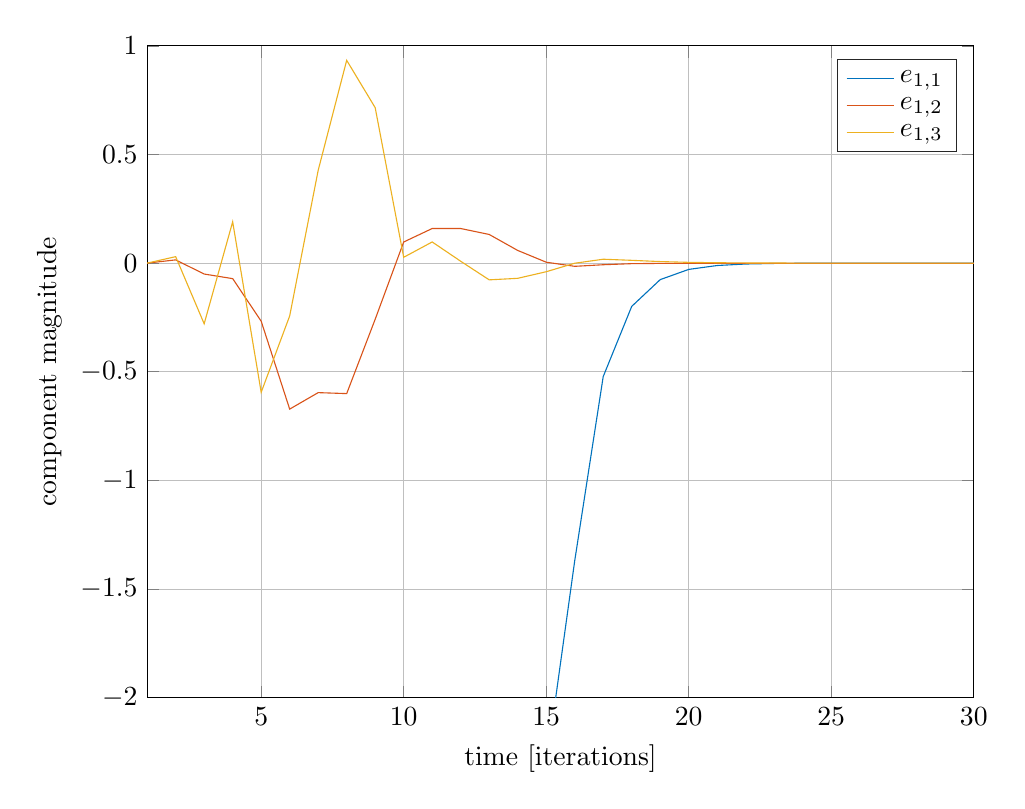
\begin{tikzpicture}

\begin{axis}[%
width=4.133in,
height=3.26in,
at={(0.693in,0.44in)},
scale only axis,
xmin=1,
xmax=30,
xmajorgrids,
ymin=-2,
ymax=1,
ymajorgrids,
xlabel={time [iterations]},
ylabel={component magnitude},
axis background/.style={fill=white},
legend style={legend cell align=left,align=left,draw=white!15!black}
]
\addplot [color=mycolor1,solid]
  table[row sep=crcr]{%
1	-12\\
2	-11.0001469447164\\
3	-10.4808387608309\\
4	-10.0065019668059\\
5	-9.0518190777714\\
6	-8.1429528224788\\
7	-7.32010620073896\\
8	-7.32563622749479\\
9	-7.00899613622404\\
10	-6.09531541589434\\
11	-5.09744679731788\\
12	-5.09744679731789\\
13	-4.29792567276087\\
14	-3.30067831532077\\
15	-2.31447961716055\\
16	-1.36978599329091\\
17	-0.521971137084024\\
18	-0.199030596012912\\
19	-0.0759440245990856\\
20	-0.0289514459189524\\
21	-0.0110371504893198\\
22	-0.00415926950700049\\
23	-0.00154905862353236\\
24	-0.000618710447507809\\
25	-0.000318924496327908\\
26	-0.000205150514504533\\
27	-0.000148861573939523\\
28	-0.000103965820983816\\
29	-8.13486002767745e-05\\
30	-5.9366284362472e-05\\
};
\addlegendentry{$\text{e}_\text{1,1}$};

\addplot [color=mycolor2,solid]
  table[row sep=crcr]{%
1	0\\
2	0.0148456863159429\\
3	-0.0502774654990725\\
4	-0.0714193369884602\\
5	-0.267154649769474\\
6	-0.671767866991735\\
7	-0.595942690548011\\
8	-0.60041446579624\\
9	-0.258256549409275\\
10	0.0971584052579576\\
11	0.159159192454583\\
12	0.159159192454582\\
13	0.131779249576538\\
14	0.0583240550487719\\
15	0.00418700699409481\\
16	-0.0148174238567389\\
17	-0.00748417651736422\\
18	-0.00253039954761965\\
19	-0.00130561839418295\\
20	-0.00105661178930735\\
21	-0.00100997478989251\\
22	-0.00100155228873798\\
23	-0.00100016068127349\\
24	-0.000999934378020436\\
25	-0.000999894969280664\\
26	-0.000999885823744575\\
27	-0.00099988279495086\\
28	-0.000999880976900566\\
29	-0.000999880223767495\\
30	-0.000999879580368125\\
};
\addlegendentry{$\text{e}_\text{1,2}$};

\addplot [color=mycolor3,solid]
  table[row sep=crcr]{%
1	0\\
2	0.0296935543194055\\
3	-0.279198422106711\\
4	0.190114513027465\\
5	-0.594562612119951\\
6	-0.243121764350111\\
7	0.426902400734066\\
8	0.933066156033846\\
9	0.715159290747244\\
10	0.0268032940088466\\
11	0.0973035972350047\\
12	0.00856149107769032\\
13	-0.0770255911312446\\
14	-0.070024749388066\\
15	-0.0396545007785583\\
16	-0.000574134892113367\\
17	0.0178728750925563\\
18	0.0128039080806008\\
19	0.00709656876859898\\
20	0.00350103116691437\\
21	0.00170563679718075\\
22	0.000743517809036174\\
23	0.000322761809562825\\
24	0.000163729709242579\\
25	9.91828081039968e-05\\
26	6.1583931768591e-05\\
27	4.60320113189769e-05\\
28	3.49578450792456e-05\\
29	3.16403528972278e-05\\
30	2.6897552973478e-05\\
};
\addlegendentry{$\text{e}_\text{1,3}$};

\end{axis}
\end{tikzpicture}%
}
      \caption{The evolution of the error states of agent 1 over time.}
      \label{fig:d_OFF_res_3_2_errors_agent_1}
    \end{figure}
  \end{minipage}
  \hfill
  \begin{minipage}{0.45\linewidth}
    \begin{figure}[H]
      \scalebox{0.7}{% This file was created by matlab2tikz.
%
%The latest updates can be retrieved from
%  http://www.mathworks.com/matlabcentral/fileexchange/22022-matlab2tikz-matlab2tikz
%where you can also make suggestions and rate matlab2tikz.
%
\definecolor{mycolor1}{rgb}{0.00000,1.00000,1.00000}%
\definecolor{mycolor2}{rgb}{0.00000,0.44700,0.74100}%
%
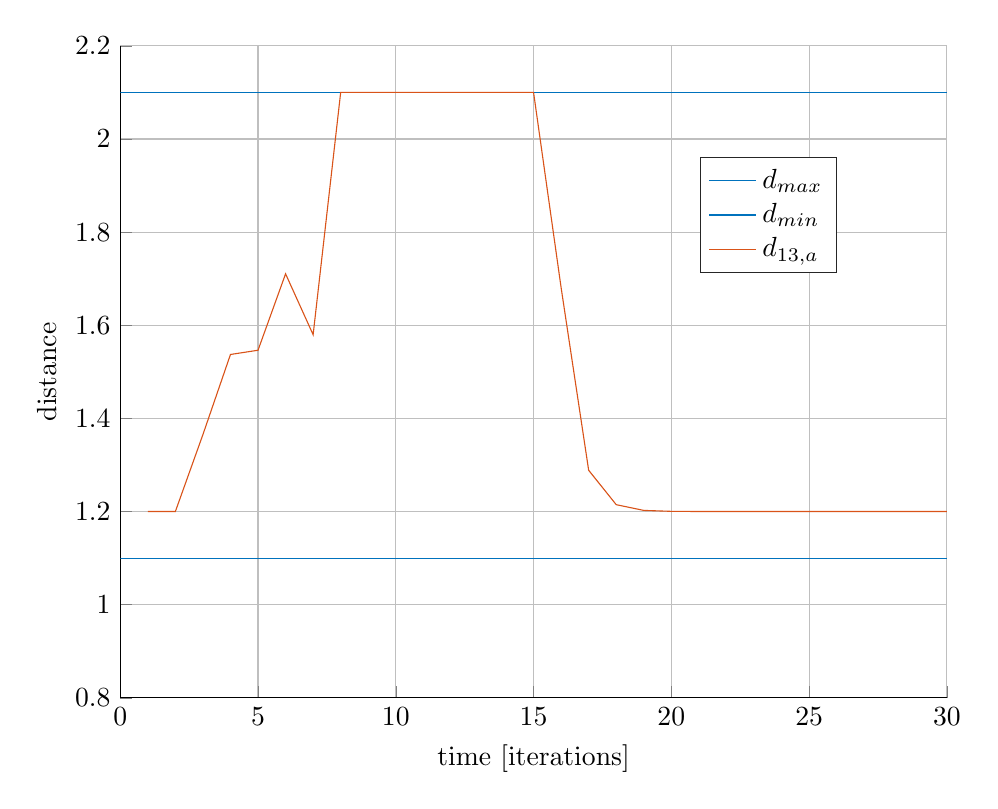
\begin{tikzpicture}

\begin{axis}[%
width=4.133in,
height=3.26in,
at={(0.693in,0.44in)},
scale only axis,
xmin=0,
xmax=30,
xmajorgrids,
ymin=0.8,
ymax=2.2,
ymajorgrids,
xlabel={time [iterations]},
ylabel={distance},
axis background/.style={fill=white},
axis x line*=bottom,
axis y line*=left,
legend style={at={(0.701,0.652)},anchor=south west,legend cell align=left,align=left,draw=white!15!black}
]
\addplot [color=mycolor1,solid]
  table[row sep=crcr]{%
0	1.1\\
30	1.1\\
};
\addlegendentry{$\text{d}_{\text{max}}$};

\addplot [color=mycolor1,solid]
  table[row sep=crcr]{%
0	2.1\\
30	2.1\\
};
\addlegendentry{$\text{d}_{\text{min}}$};

\addplot [color=mycolor2,solid]
  table[row sep=crcr]{%
1	1.2\\
2	1.19999732077084\\
3	1.36521091151\\
4	1.53723482189595\\
5	1.54632534062289\\
6	1.71036961929341\\
7	1.57966816234267\\
8	2.09999999985556\\
9	2.0999999999955\\
10	2.09999999999102\\
11	2.09999999977532\\
12	2.1\\
13	2.09999999995514\\
14	2.09999999986519\\
15	2.09999999999797\\
16	1.68077678659047\\
17	1.28856266207741\\
18	1.21470405925992\\
19	1.20240233406648\\
20	1.20039387372556\\
21	1.20006432186432\\
22	1.20001005795673\\
23	1.20000154705776\\
24	1.20000022333303\\
25	1.19999999462576\\
26	1.19999992479106\\
27	1.19999989994857\\
28	1.19999988715586\\
29	1.19999988107988\\
30	1.19999987794025\\
};
\addlegendentry{$\text{d}_{\text{13,a}}$};

\end{axis}
\end{tikzpicture}%
}
      \caption{The distance between agents 1 and 3 over time. The maximum allowed
        distance has a value of $2.1$ and the minimum allowed distance a value
        of $1.1$.}
  \label{fig:d_OFF_res_3_2_distance_agents_13}
    \end{figure}
  \end{minipage}
\end{minipage}
}

\noindent\makebox[\linewidth][c]{%
\begin{minipage}{\linewidth}
  \begin{minipage}{0.45\linewidth}
    \begin{figure}[H]
      \scalebox{0.7}{% This file was created by matlab2tikz.
%
%The latest updates can be retrieved from
%  http://www.mathworks.com/matlabcentral/fileexchange/22022-matlab2tikz-matlab2tikz
%where you can also make suggestions and rate matlab2tikz.
%
\definecolor{mycolor1}{rgb}{0.00000,0.44700,0.74100}%
\definecolor{mycolor2}{rgb}{0.85000,0.32500,0.09800}%
\definecolor{mycolor3}{rgb}{0.92900,0.69400,0.12500}%
\definecolor{mycolor4}{rgb}{0.00000,1.00000,1.00000}%
%
\begin{tikzpicture}

\begin{axis}[%
width=4.133in,
height=3.26in,
at={(0.693in,0.44in)},
scale only axis,
xmin=0,
xmax=30,
xmajorgrids,
ymin=1.2,
ymax=7,
ymajorgrids,
xlabel={time [iterations]},
ylabel={distance},
axis background/.style={fill=white},
axis x line*=bottom,
axis y line*=left,
legend style={at={(0.709,0.51)},anchor=south west,legend cell align=left,align=left,draw=white!15!black}
]
\addplot [color=mycolor1,solid]
  table[row sep=crcr]{%
1	6.32455532033676\\
2	5.37980549071204\\
3	4.92763165081336\\
4	4.51030332457465\\
5	3.80178772282473\\
6	3.4249949393334\\
7	2.91231846367102\\
8	2.91881256704999\\
9	2.47341784700138\\
10	1.90522732585578\\
11	2.05019442063337\\
12	2.05019442063337\\
13	2.52731196882367\\
14	3.3251230101429\\
15	4.19122058538753\\
16	5.04959117151099\\
17	5.83427741386267\\
18	6.13688634627583\\
19	6.2529723634364\\
20	6.29743188917348\\
21	6.31440550899511\\
22	6.32092661543391\\
23	6.32340219653524\\
24	6.32428467060215\\
25	6.32456904361269\\
26	6.32467697032657\\
27	6.32473036691825\\
28	6.32477295597452\\
29	6.32479441120973\\
30	6.32481526419489\\
};
\addlegendentry{$\text{d}_{\text{1,o}_\text{2}}$};

\addplot [color=mycolor2,solid]
  table[row sep=crcr]{%
1	6.8\\
2	6.4053632492008\\
3	6.2552251757312\\
4	5.8609810822034\\
5	5.40622455899826\\
6	5.00689533638028\\
7	5.01018244486427\\
8	4.47839241411677\\
9	3.53966570373938\\
10	2.62355069277046\\
11	1.80903430565789\\
12	1.98973871951536\\
13	2.10457417241241\\
14	2.66664801496521\\
15	3.49542704716424\\
16	4.39621016228712\\
17	5.33777091437137\\
18	6.27070065306331\\
19	6.62474535854054\\
20	6.74870510812654\\
21	6.78790010040939\\
22	6.79862933361955\\
23	6.80061297472504\\
24	6.80049553533332\\
25	6.80013457757052\\
26	6.79992331083544\\
27	6.79979031829651\\
28	6.79971190113048\\
29	6.79965937653708\\
30	6.7996105569016\\
};
\addlegendentry{$\text{d}_{\text{2,o}_\text{2}}$};

\addplot [color=mycolor3,solid]
  table[row sep=crcr]{%
1	6.05309838016862\\
2	5.06141684134664\\
3	4.07417165620072\\
4	3.14267168759638\\
5	2.31314449241178\\
6	1.71471478283139\\
7	1.6\\
8	1.78675250315056\\
9	1.96762715208123\\
10	2.50957758755285\\
11	3.26589672246329\\
12	3.26589672264825\\
13	3.91981984551029\\
14	4.73294699335171\\
15	5.53328341549778\\
16	5.86628630465754\\
17	5.99171607388954\\
18	6.03529344464427\\
19	6.04901351578096\\
20	6.05285729669339\\
21	6.05360002859138\\
22	6.05357042196635\\
23	6.0534926996183\\
24	6.05343740282609\\
25	6.05339981823955\\
26	6.05334370739466\\
27	6.05330884627764\\
28	6.05328807107311\\
29	6.05326494865147\\
30	6.05325605718366\\
};
\addlegendentry{$\text{d}_{\text{3,o}_\text{2}}$};

\addplot [color=mycolor4,solid]
  table[row sep=crcr]{%
0	1.6\\
30	1.6\\
};
\addlegendentry{$\text{d}_{\text{min}}$};

\end{axis}
\end{tikzpicture}%
}
      \caption{The distance between each agent and obstacle 2 over time. The
        minimum allowed distance has a value of $1.6$.}
      \label{fig:d_OFF_res_3_2_distance_obstacle_2_agents}
    \end{figure}
  \end{minipage}
  \hfill
  \begin{minipage}{0.45\linewidth}
    \begin{figure}[H]
      \scalebox{0.7}{% This file was created by matlab2tikz.
%
%The latest updates can be retrieved from
%  http://www.mathworks.com/matlabcentral/fileexchange/22022-matlab2tikz-matlab2tikz
%where you can also make suggestions and rate matlab2tikz.
%
\definecolor{mycolor1}{rgb}{0.00000,0.44700,0.74100}%
\definecolor{mycolor2}{rgb}{0.85000,0.32500,0.09800}%
%
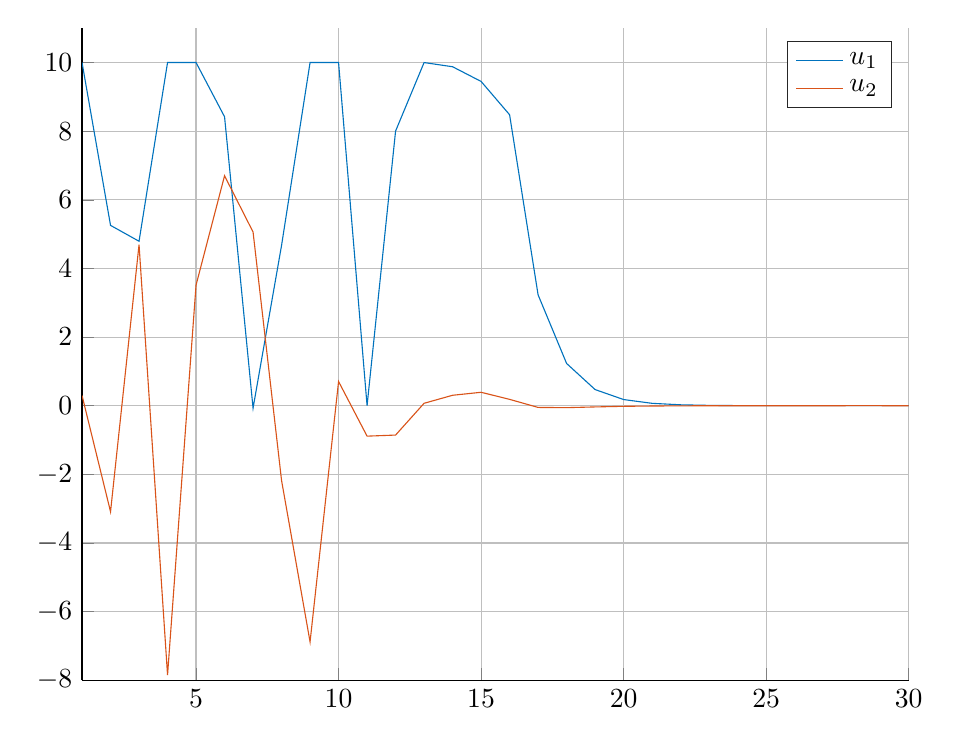
\begin{tikzpicture}

\begin{axis}[%
width=4.133in,
height=3.26in,
at={(0.693in,0.44in)},
scale only axis,
xmin=1,
xmax=30,
xmajorgrids,
ymin=-8,
ymax=11,
ymajorgrids,
axis background/.style={fill=white},
axis x line*=bottom,
axis y line*=left,
legend style={legend cell align=left,align=left,draw=white!15!black}
]
\addplot [color=mycolor1,solid]
  table[row sep=crcr]{%
1	10\\
2	5.25462130162317\\
3	4.79193319738521\\
4	10\\
5	10\\
6	8.4199467228726\\
7	-0.0718830937370075\\
8	4.6711348570471\\
9	10\\
10	10\\
11	-7.94569359373262e-14\\
12	8.00234026799899\\
13	9.99951019516972\\
14	9.87721457016684\\
15	9.44944892693392\\
16	8.47858591990533\\
17	3.22978879082904\\
18	1.23092831962601\\
19	0.469932637132582\\
20	0.179143585415878\\
21	0.0687788640459975\\
22	0.0261021127368294\\
23	0.00930348204528589\\
24	0.00299785953822199\\
25	0.0011377398219765\\
26	0.00056288940647063\\
27	0.000448957529927465\\
28	0.000226172207195904\\
29	0.000219823159237385\\
30	0.000355769756634746\\
};
\addlegendentry{$\text{u}_\text{1}$};

\addplot [color=mycolor2,solid]
  table[row sep=crcr]{%
1	0.296935543194055\\
2	-3.08891976426117\\
3	4.69312935134176\\
4	-7.84677125147416\\
5	3.5144084776984\\
6	6.70024165084176\\
7	5.06163755299781\\
8	-2.17906865286603\\
9	-6.88355996738395\\
10	0.705003032261582\\
11	-0.887421061573144\\
12	-0.855870822089348\\
13	0.0700084174317851\\
14	0.303702486095077\\
15	0.390803658864449\\
16	0.184470099846696\\
17	-0.0506896701195546\\
18	-0.0570733931200179\\
19	-0.035955376016846\\
20	-0.0179539436973362\\
21	-0.0096211898814456\\
22	-0.0042075599947334\\
23	-0.00159032100320243\\
24	-0.000645469011385813\\
25	-0.000375988763354052\\
26	-0.000155519204496137\\
27	-0.000110741662397311\\
28	-3.31749218201766e-05\\
29	-4.74279992374978e-05\\
30	-8.91179333348645e-05\\
};
\addlegendentry{$\text{u}_\text{2}$};

\end{axis}
\end{tikzpicture}%}
      \caption{The inputs signals directing agent 1 over time. Their value is
        constrained between $-10$ and $10$.}
      \label{fig:d_OFF_res_3_2_inputs_agent_1}
    \end{figure}
  \end{minipage}
\end{minipage}
}
